% !TEX root = ../Appunti_Fisica_2.tex
\documentclass[11pt,oneside]{scrbook} % KOMA: pulito e flessibile

% ---------- LINGUA & CODIFICA ----------
\usepackage[italian]{babel}
\usepackage[T1]{fontenc}
\usepackage[utf8]{inputenc}
\usepackage{csquotes}

% ---------- TIPOGRAFIA CONSIGLIATA ----------
\usepackage{lmodern}     % font semplice e diffuso
\usepackage{microtype}   % micro-tipografia, migliore resa

% ---------- FIGURE IN TIKZ -----------

\usepackage{tikz}
\usetikzlibrary{arrows.meta, patterns, decorations.markings, decorations.pathmorphing, calc, positioning}
\usepackage{amsmath, amssymb, bm}

% Stile coerente con le immagini a colori
\definecolor{posred}{RGB}{239,130,140}   % rosa-rosso per cariche positive
\definecolor{negblue}{RGB}{120,190,230}  % azzurro per cariche negative
\definecolor{ered}{RGB}{227,35,35}       % rosso vivo per i vettori E
\definecolor{surfblue}{RGB}{205,230,245} % azzurro chiaro per la superficie
\definecolor{gray60}{gray}{0.55}
\definecolor{blobpink}{RGB}{245,205,190} % colore del corpo esteso
\definecolor{cubecol}{RGB}{235,190,170}
\definecolor{charge}{RGB}{245,175,120}      % arancione chiaro delle cariche
\definecolor{matpink}{RGB}{245,210,195}     % superficie superiore del materiale
\definecolor{matpinkdk}{RGB}{225,175,155}   % fianco laterale
\definecolor{loopblue}{RGB}{90,130,200}     % anelli di corrente
\definecolor{mred}{RGB}{227,35,35}          % vettore M
\definecolor{surrfblue}{RGB}{190,215,235}   % regione chiusa C (riempimento)
\definecolor{surfedge}{RGB}{80,120,170}     % bordo della curva C
\definecolor{ghost}{RGB}{140,140,140}       % traslazione (tratteggiata)
\definecolor{vred}{RGB}{227,35,35}          % vettori v



% ---------- GEOMETRIA PAGINA ----------
% Scegli *una* delle due geometrie qui sotto.
% (1) Impostazioni consigliate per A4 (Italia) con ampio margine esterno:
\usepackage[
  a4paper,
  top=24mm,
  bottom=28mm,
  inner=28mm,   % margine interno (verso rilegatura)
  outer=50mm,   % margine esterno: ampio per le note a margine
  heightrounded
]{geometry}
\setlength{\headheight}{17pt} % evita sovrapposizioni con l'header
\setlength{\headsep}{6mm}     % distanza tra header e corpo


% (2) Se vuoi replicare il formato del PDF caricato (US Letter 8.5x11"):
% \usepackage[
%   letterpaper,
%   top=25mm,
%   bottom=30mm,
%   inner=30mm,
%   outer=55mm,
%   heightrounded
% ]{geometry}

% ---------- HEADER/FOOTER ----------
\usepackage{fancyhdr}
\pagestyle{fancy}
\fancyhf{} % pulisci

% intestazione: solo titolo del capitolo (sinistra), pagina a destra
\fancyhead[L]{\nouppercase{\leftmark}}
\fancyfoot[R]{\thepage}

\renewcommand{\headrulewidth}{0.4pt}
\renewcommand{\footrulewidth}{0pt}

\fancypagestyle{plain}{%
  \fancyhf{}
  \fancyfoot[R]{\thepage}
  \renewcommand{\headrulewidth}{0pt}
}

% ---------- STRUMENTI DI STRUTTURA ----------
\setcounter{secnumdepth}{3}
\setcounter{tocdepth}{2}
\usepackage{titlesec}

% --- Titoli puliti ---
% Capitolo
\titleformat{\chapter}[display]
  {\normalfont\huge\bfseries}
  {\thechapter}{1ex}{}
\titlespacing*{\chapter}{0pt}{-0.5em}{1.5ex}

% Capitolo
\titleformat{\chapter}[display]
  {\normalfont\huge\bfseries}
  {\thechapter}{1ex}{}
\titlespacing*{\chapter}{0pt}{1.5ex}{1.5ex}

% Sezione
\titleformat{\section}
  {\normalfont\Large\bfseries}
  {\thesection}{1em}{}

% Sottosezione
\titleformat{\subsection}
  {\normalfont\large\bfseries}
  {\thesubsection}{0.8em}{}

% SOTTO-sottosezione  <--- AGGIUNGI QUESTO BLOCCO
\titleformat{\subsubsection}
  {\normalfont\normalsize\bfseries}
  {\thesubsubsection}{0.8em}{}
\titlespacing*{\subsubsection}{0pt}{0.8ex}{0.4ex}

% ---------- PAGINA SEPARATRICE ----------
\newcommand{\partpage}[1]{%
  \cleardoublepage          % vai a pagina nuova (pari se oneside)
  \thispagestyle{empty}     % niente header/footer
  \null\vfill               % spazio verticale elastico sopra
  \begin{center}
    {\Huge\bfseries #1}
  \end{center}
  \vfill\null               % spazio verticale elastico sotto
  \cleardoublepage          % lascia la pagina successiva libera
}

% ---------- AMBIENTI UTILI ----------
\usepackage{amsmath,amssymb,amsthm}
\usepackage{graphicx}
\usepackage[hidelinks]{hyperref}
\usepackage{xcolor}
\usepackage{tcolorbox}
\usepackage{subcaption} 

% ---------- NOTE A MARGINE (parole-chiave/sidenote) ----------
% \marginpar stampa nel margine esterno con oneside.
% Definiamo un comando comodo e graficamente coerente:
\newcommand{\mkeyword}[1]{%
  \marginpar{\raggedright\footnotesize\emph{#1}}%
}

% Se preferisci le note a sinistra, attiva la riga seguente:
% \reversemarginpar

% ---------- PARAGRAFI E SPAZI ----------
\setlength{\parindent}{0.8em}  % rientro tradizionale
\setlength{\parskip}{0.25em}   % piccolo spazio extra tra paragrafi

%----------- COMANDI AGGIUNTIVI -----------
% --- Comando per vettori colonna di lunghezza variabile ---

\newcommand{\colvec}[1]{%
  \begin{pmatrix}
    #1
  \end{pmatrix}%
}

\renewcommand{\Re}{\operatorname{Re}}
\renewcommand{\Im}{\operatorname{Im}}

\newcommand{\FIG}[1]{
  \begin{figure}[h]
    \centering
    \includegraphics[width=0.4\linewidth]{figure/image#1.png}
    \caption{}
    \label{}
  \end{figure}
}

\newcommand{\eps}{\varepsilon}

% ---------- BIBLIOGRAFIA ----------
\usepackage[backend=biber,style=numeric,sorting=nyt]{biblatex}
\addbibresource{bibliografia.bib} % nome del file .bib

% ---------- FRONTESPIZIO ----------
\title{\textbf{Appunti di Fisica 2}}
\author{Roberto Riccucci}
\date{}

\publishers{
  Email: \text{roberto.riccucci1304@gmail.com} \\
  Versione: v0.1
}



\begin{document}

\frontmatter

\frontmatter

\newgeometry{
    a4paper,
    top=24mm,
    bottom=28mm,
    left=39mm,
    right=39mm,
    heightrounded
}
\begin{titlepage}
    \centering

    \makebox[\textwidth][c]{\Huge\bfseries Appunti di Fisica 2 \par}

    \vspace{1cm}

    \makebox[\textwidth][c]{\Large Roberto Riccucci \par}

    \vspace{1.5cm}

    \makebox[\textwidth][c]{\rule{0.8\textwidth}{0.4pt}}

    \vspace{0.7cm}

    \makebox[\textwidth][c]{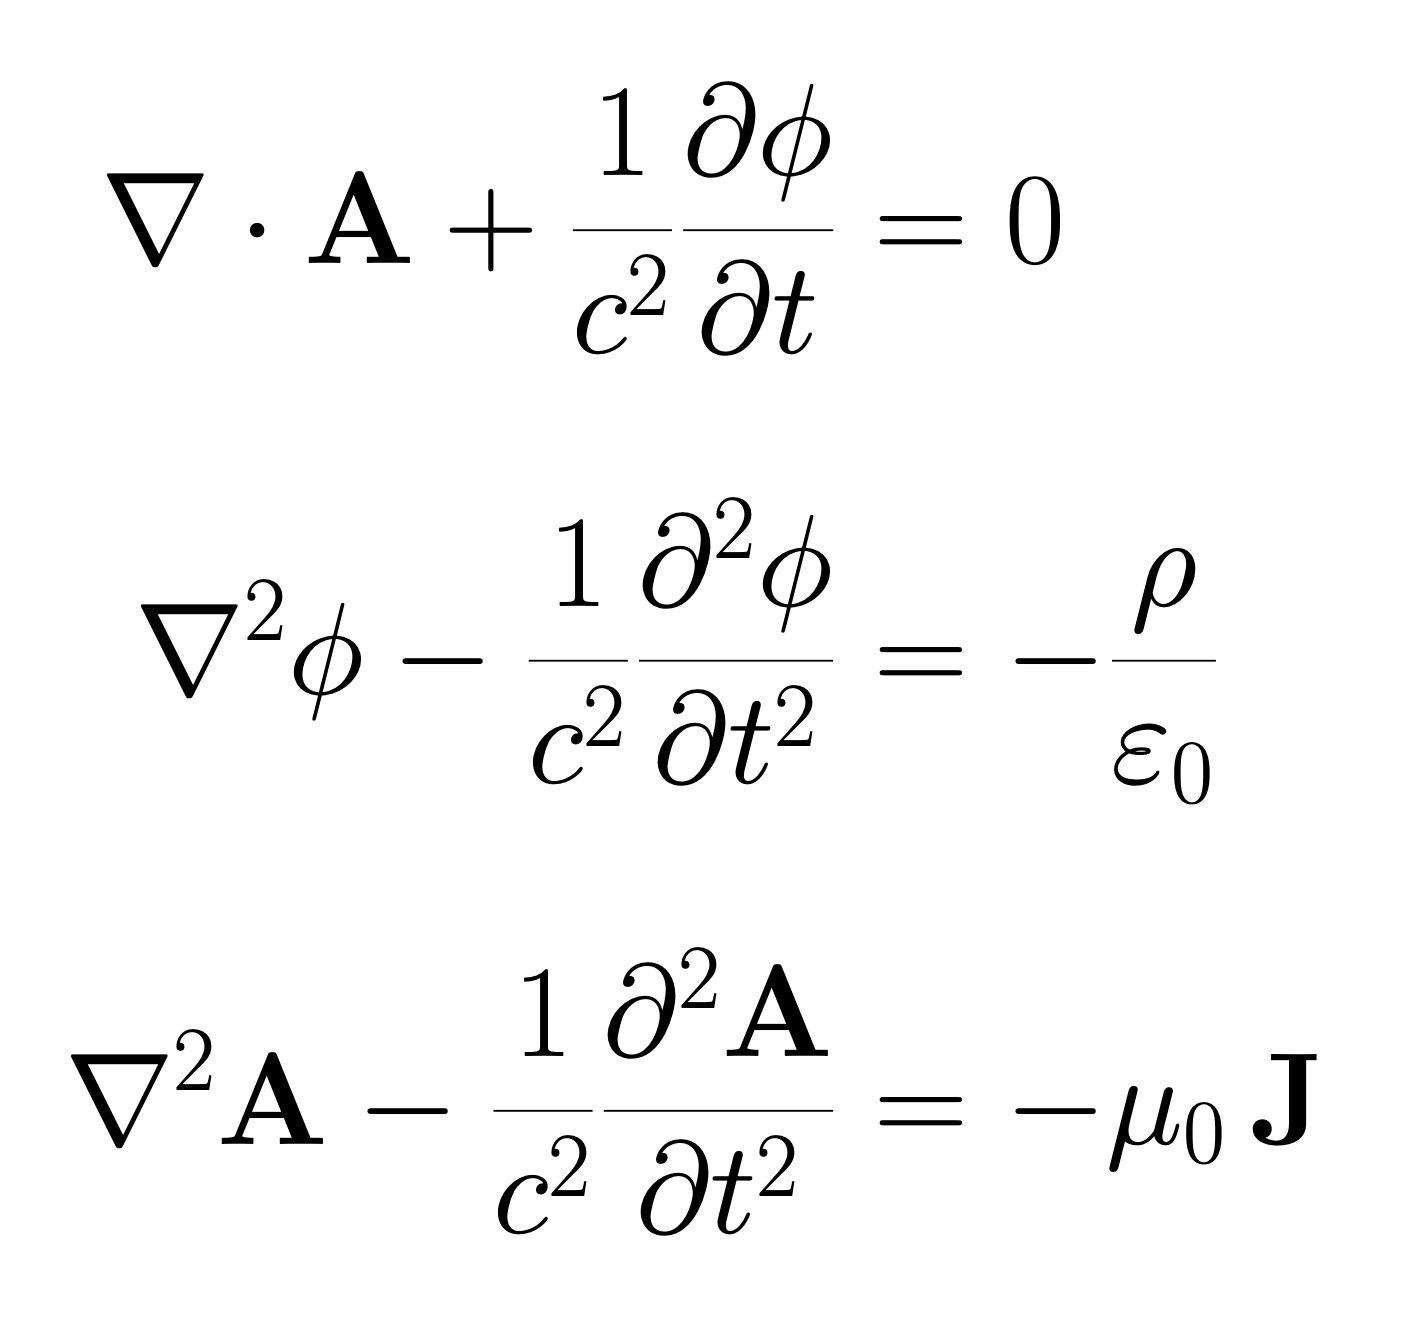
\includegraphics[width=0.7\textwidth]{figure/image62.png}}

    \vspace{0.7cm}

    \makebox[\textwidth][c]{\rule{0.8\textwidth}{0.4pt}}

    \vfill

    \makebox[\textwidth][c]{\large Versione v0.1 \par}
    \makebox[\textwidth][c]{\small robertoriccucci1304@gmail.com \par}

\end{titlepage}
\restoregeometry

% !TEX root = ../Appunti_Fisica_2.tex
\addchap{Prefazione}
Queste note nascono come riferimento per lo studio del corso di \emph{Fisica 2}, tenuto dal professor Francesco Forti. Il contenuto segue prevalentemente il programma svolto nell'anno scolastico 2025/2026, per cui non è garantito che rimanga valido anche per gli anni successivi. \\
Le presenti note sono state scritte con due obiettivi principali: riportare in un unico testo tutto il programma dell'intero anno e riportare in forma più compatta teoremi e dimostrazioni presenti nei libri: \emph{"Classical Electrodynamics"} di \emph{John David Jackson}, \emph{"Introduction to Electrodynamics"} di \emph{David J. Griffiths} e \emph{"Fisica - Volume II - Elettromagnetismo e Onde"} di \emph{P. Mazzoldi, M. Nigro, C. Voci}, che sono \textbf{i testi principali utilizzati per scrivere questi appunti}.\\

\' E importante sottolineare che sono presenti approfondimenti non svolti a lezione ma spiegati nei corsi di \emph{Elettrodinamica 1} ed \emph{Elettrodimanica 2} tenuti alla Scuola Normale Superiore dal professore Giuseppe Carlo La Rocca. \\

Non sempre gli argomenti seguiranno l'ordine delle lezioni. \\

Questi appunti, insieme al codice \LaTeX{} e a tutte le immagini, sono disponibili sulla mia pagina GitHub: \url{https://github.com/RobertoRiccucci}.

\begin{flushright}
Roberto Riccucci\\
Pisa, \today
\end{flushright}

\tableofcontents


% --- FORMULARIO: Operazioni vettoriali in vari sistemi di coordinate ---
\addchap{Forme esplicite di operazioni vettoriali}

Siano $\mathbf e_1,\mathbf e_2,\mathbf e_3$ i tre versori mutuamente ortogonali delle direzioni
coordinate indicate nella colonna a sinistra, ed $A_1,A_2,A_3$ le corrispondenti componenti di un
vettore $\mathbf A$. Allora:

% Stile comune per i riquadri
\tcbset{
  colback=white,
  boxrule=0.6pt,
  colframe=black,
  width=\textwidth,  % <-- larghezza piena
  left=6pt, right=6pt, top=4pt, bottom=4pt,
  rounded corners,
  % 'enhanced' removed because it's not available in this tcolorbox version
  before skip=10pt,
  after skip=10pt
  }

% -------- CARTESIANE --------
\begin{tcolorbox}[title={\normalsize \textbf{Coordinate cartesiane} \ $(x_1,x_2,x_3)$}]
\[
\nabla \psi = \mathbf e_1\,\frac{\partial \psi}{\partial x_1}
            + \mathbf e_2\,\frac{\partial \psi}{\partial x_2}
            + \mathbf e_3\,\frac{\partial \psi}{\partial x_3}
\]
\[
\nabla\!\cdot\!\mathbf A = \frac{\partial A_1}{\partial x_1}
                         + \frac{\partial A_2}{\partial x_2}
                         + \frac{\partial A_3}{\partial x_3}
\]
\[
\nabla\!\times\!\mathbf A =
\mathbf e_1\!\left(\frac{\partial A_3}{\partial x_2}-\frac{\partial A_2}{\partial x_3}\right)
+ \mathbf e_2\!\left(\frac{\partial A_1}{\partial x_3}-\frac{\partial A_3}{\partial x_1}\right)
+ \mathbf e_3\!\left(\frac{\partial A_2}{\partial x_1}-\frac{\partial A_1}{\partial x_2}\right)
\]
\[
\nabla^2 \psi=\frac{\partial^2\psi}{\partial x_1^2}
             + \frac{\partial^2\psi}{\partial x_2^2}
             + \frac{\partial^2\psi}{\partial x_3^2}
\]
\end{tcolorbox}

% -------- CILINDRICHE --------
\begin{tcolorbox}[title={\normalsize \textbf{Coordinate cilindriche} \ $(\rho,\varphi,z)$}]
\[
\nabla \psi = \mathbf e_\rho\,\frac{\partial \psi}{\partial \rho}
            + \mathbf e_\varphi\,\frac{1}{\rho}\frac{\partial \psi}{\partial \varphi}
            + \mathbf e_z\,\frac{\partial \psi}{\partial z}
\]
\[
\nabla\!\cdot\!\mathbf A =
\frac{1}{\rho}\frac{\partial}{\partial \rho}\!\big(\rho A_\rho\big)
+ \frac{1}{\rho}\frac{\partial A_\varphi}{\partial \varphi}
+ \frac{\partial A_z}{\partial z}
\]
\[
\nabla\!\times\!\mathbf A =
\mathbf e_\rho\!\left(\frac{1}{\rho}\frac{\partial A_z}{\partial \varphi}-\frac{\partial A_\varphi}{\partial z}\right)
+ \mathbf e_\varphi\!\left(\frac{\partial A_\rho}{\partial z}-\frac{\partial A_z}{\partial \rho}\right)
+ \mathbf e_z\!\left(\frac{1}{\rho}\frac{\partial}{\partial \rho}(\rho A_\varphi)-\frac{1}{\rho}\frac{\partial A_\rho}{\partial \varphi}\right)
\]
\[
\nabla^2\psi=\frac{1}{\rho}\frac{\partial}{\partial \rho}\!\left(\rho\,\frac{\partial\psi}{\partial \rho}\right)
            + \frac{1}{\rho^2}\frac{\partial^2\psi}{\partial \varphi^2}
            + \frac{\partial^2\psi}{\partial z^2}
\]
\end{tcolorbox}

% -------- SFERICHE --------
\begin{tcolorbox}[title={\normalsize \textbf{Coordinate sferiche} \ $(r,\theta,\varphi)$}]
\[
\nabla \psi = \mathbf e_r\,\frac{\partial \psi}{\partial r}
            + \mathbf e_\theta\,\frac{1}{r}\frac{\partial \psi}{\partial \theta}
            + \mathbf e_\varphi\,\frac{1}{r\sin\theta}\frac{\partial \psi}{\partial \varphi}
\]
\[
\nabla\!\cdot\!\mathbf A =
\frac{1}{r^2}\frac{\partial}{\partial r}\!\big(r^2 A_r\big)
+ \frac{1}{r\sin\theta}\frac{\partial}{\partial \theta}\!\big(\sin\theta\, A_\theta\big)
+ \frac{1}{r\sin\theta}\frac{\partial A_\varphi}{\partial \varphi}
\]

\begin{align*}
    \nabla\!\times\!\mathbf A =
\mathbf e_r\,\frac{1}{r\sin\theta}\!\left[\frac{\partial}{\partial \theta}(A_\varphi\sin\theta)-\frac{\partial A_\theta}{\partial \varphi}\right]
+ \mathbf e_\theta\,\frac{1}{r}\!\left[\frac{1}{\sin\theta}\frac{\partial A_r}{\partial \varphi}-\frac{\partial}{\partial r}(rA_\varphi)\right] + \\ 
+ \mathbf e_\varphi\,\frac{1}{r}\!\left[\frac{\partial}{\partial r}(rA_\theta)-\frac{\partial A_r}{\partial \theta}\right] \quad \quad \quad \quad \quad \quad \quad \quad \quad  \quad
\end{align*}



\[
\nabla^2\psi=\frac{1}{r^2}\frac{\partial}{\partial r}\!\left(r^2\frac{\partial \psi}{\partial r}\right)
            + \frac{1}{r^2\sin\theta}\frac{\partial}{\partial \theta}\!\left(\sin\theta\,\frac{\partial \psi}{\partial \theta}\right)
            + \frac{1}{r^2\sin^2\theta}\frac{\partial^2\psi}{\partial \varphi^2}
\]
\end{tcolorbox}

\mainmatter

% !TEX root = ../Appunti_Fisica_2.tex

\newgeometry{
    a4paper,
    top=24mm,
    bottom=28mm,
    left=39mm,
    right=39mm,
    heightrounded
}
\partpage{Elettrostatica}
\restoregeometry

\chapter{Forza elettrostatica e Campo elettrostatico}

Un' \emph{interazione} fondamentale, che gioca un ruolo essenziale nella costruzione della materia, è quella elettromagnetica. Un aspetto particolare dell'interazione elettromagnetica è la \emph{forza elettrica} \mkeyword{forza elettrica}: le sue proprietà costituiscono l'argomento dei primi capitoli di questi appunti. \\

La formulazione precisa della legge della forza elettrica è dovuta a Coulomb, il quale eseguì nel 1785 una serie di misure sistematiche per stabilire la dipendenza della forza tra due cariche dai valori $q_1$ e $q_2$ di queste e dalla loro distanza $r$.\\ 
\mkeyword{Legge di Coulomb} Coulomb stabilì che due \emph{cariche puntiformi} $q_1$ e $q_2$, poste a distanza $r$, interagiscono con una forza $\mathbf{F}$, diretta secondo la loro congiungente, di modulo 

\begin{equation}
    F = k \frac{q_1 \ q_2}{r^2}
\end{equation}

Quindi la forza elettrostatica è direttamente proporzionale al prodotto delle cariche elettriche e inversamente proporzionale al quadrato della loro distanza. \\

L'unità di misura della carica elettrica è il coulomb, simbolo C \mkeyword{coulomb (C)}, che è pari alla carica trasportata in 1 secondo da una corrente di 1A.\\

Il valore di k nel vuoto risulta 

\begin{equation*}
    k = 8.99 \cdot 10^9 \ Nm^2/C^2 \approx 9 \cdot 10^9 \ Nm^2/C^2
\end{equation*}

Per ragioni pratiche è conveniente scrivere k come:

\begin{equation*}
    k = \frac{1}{4 \pi \varepsilon_0}
\end{equation*}

dove la costante $\varepsilon_0$ è nota come costante dielettrica \mkeyword{costante dielettrica} e ha il valore 

\begin{equation*}
    \varepsilon_0 = 8.85 \cdot 10^{-12} \ \frac{C^2}{Nm^2}
\end{equation*}

A seguito dell'ultima ridefinizione del Sistema Internazionale, il valore della carica elementare \mkeyword{carica elementare} espresso in Coulomb è fissato pari a 

\begin{equation*}
    e = 1.602 \cdot 10^{-19} C
\end{equation*}

\newpage

Allora considerate due cariche $q$ e $q_0$ possiamo scrivere la forza elettrostatica che la carica $q$ esercita sulla carica $q_0$ come

\begin{tcolorbox}[colback=yellow!10!white, colframe=orange!70!black, boxrule=0.8pt]
\begin{equation}
    \mathbf{F} = \frac{1}{4 \pi \varepsilon_0} \ \frac{q \ q_0}{r^2} \mathbf{u}
\end{equation}
\end{tcolorbox}

Dove $\mathbf{u}$ è il versore del vettore $\mathbf{r}$ che va da $q$ a $q_0$.\\

\section{Campo elettrostatico}

Le forze elettriche agenti su una carica $q_0$ dovute alle cariche circostanti si sommano come vettori: vige cioè il principio di sovrapposizione \mkeyword{principio di sovrapposizione}, pertanto possiamo scrivere. 

\begin{equation*}
    \mathbf{F} = \sum_i \mathbf{F}_i = q_0 \sum_i \frac{1}{4 \pi \varepsilon_0} \ \frac{q_i}{r_i^2} \mathbf{u}_i
\end{equation*}

Si nota così che la forza elettrica risultante esercitata su $q_0$ è proporzionale a $q_0$. \\
Possiamo andare così a definire la grandezza vettoriale 

\begin{tcolorbox}[colback=yellow!10!white, colframe=orange!70!black, boxrule=0.8pt]
\begin{equation}
    \mathbf{E} = \frac{\mathbf{F}}{q_0}
\end{equation}
\end{tcolorbox}

che prende il nome di campo elettrico \mkeyword{campo elettrico}.\\
L'unità di misura del campo elettrico è $N/C$

E quindi dalla legge di Coulomb si ottiene:

\begin{equation}
    \mathbf{E}(x,y,z) = \sum_i \frac{1}{4 \pi \varepsilon_0} \ \frac{q_i}{r_i ^2} \mathbf{u}_i
    \label{eq: campo elettrostatico}
\end{equation}

Il campo elettrostatico in un punto $P$ prodotto da un sistema discreto di cariche è uguale alla somma dei campi elettrostatici prodotti singolarmente dalle cariche. 

\begin{figure} [h]
    \centering
    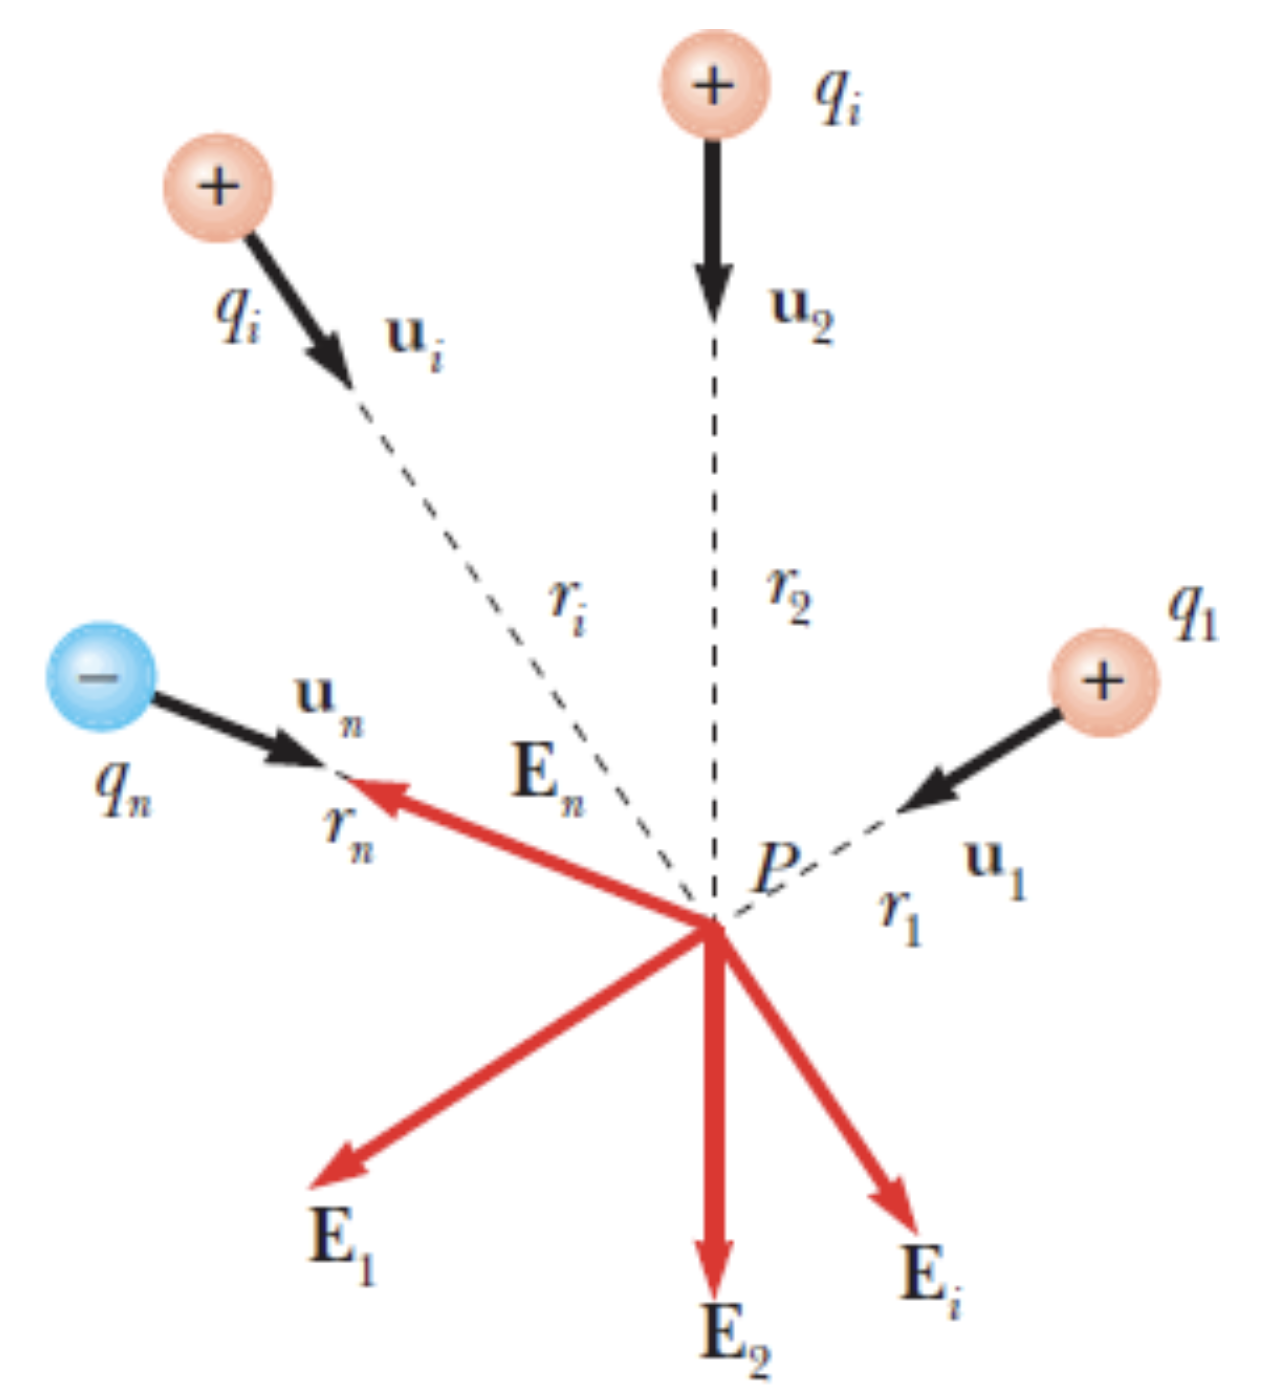
\includegraphics[width=0.4\linewidth]{figure/image1.png}
    \caption{Campo elettrostatico di un sistema discreto di cariche}
    \label{fig:chapter_1_1}
\end{figure}

Le cariche di interesse nei problemi corrispondono a un numero molto grande di cariche elementari, inoltre nella maggior parte dei casi queste non sono concentrate in un unico punto, ma sono distribuite nello spazio con una ben determinata geometria.\\

Supponendo che $\rho (x,y,z)$ sia la densità spaziale di carica, possiamo modificare la \ref{eq: campo elettrostatico} in modo da passare dal caso discreto a quello continuo.

\begin{tcolorbox}[colback=yellow!10!white, colframe=orange!70!black, boxrule=0.8pt]
\begin{equation}
    \mathbf{E}(x,y,z) = \frac{1}{4 \pi \varepsilon_0} \int_V \frac{dq}{r^2} \mathbf{u} =  \frac{1}{4 \pi \varepsilon_0} \int_V \frac{\rho(x,y,z)}{r^2} dV \mathbf{u}
    \label{eq:campo_elettrostatico_continuo}
\end{equation}
\end{tcolorbox}

Lo stesso vale anche per i casi in cui si stia trattando con densità superficiali e lineari di carica. 

\begin{figure} [h]
    \centering
    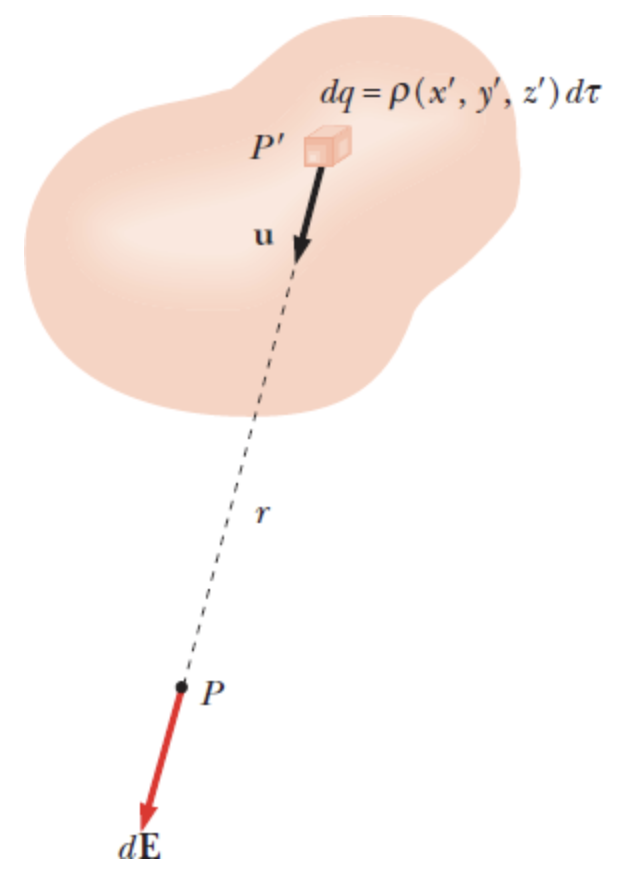
\includegraphics[width=0.4\linewidth]{figure/image3.png}
    \caption{Campo elettrostatico prodotto da un elemento di una distribuzione di carica}
    \label{fig:chapter_1_2}
\end{figure}

\subsection{Linee di forza del campo elettrostatico}

Partendo da una generica posizione e muovendosi per tratti infinitesimi successivi, ciascuno parallelo e concorde al campo elettrostatico in quel dato punto, si ottiene una linea che è detta linea di forza o linea del campo elettrostatico. \mkeyword{linea di forza}\\

Già a questo punto si possono desumere le proprietà delle linee di forza:

\begin{enumerate}
    \item le linee di forza non si incrociano mai, in quanto in ogni punto il campo è definito univocamente e non può avere due direzioni distinte;
    \item le linee di forza hanno origine dalle cariche positive e terminano sulle cariche negative, qualora ci siamo cariche di uno stesso segno le linee di forza si chiudono all'infinito. 
\end{enumerate}


\chapter{Lavoro elettrico e Potenziale elettrostatico}

Come vedremo nel seguito, se una carico $q_0$ si muove in presenza di altre cariche, sia fisse che in moto, \emph{la forza su di essa è sempre proporzionale a $q_0$}. Più in generale, quando su una carica $q_0$ agisce una forza $\mathbf{F}$ di qualsiasi natura, non necessariamente elettrostatica, ma ad esempio dovuta a processi chimici o ad azioni meccaniche, o ad altre cause ancora, possiamo definire sempre un campo elettrico $\mathbf{E}$, che si indica con il nome di campo elettromotore \mkeyword{campo elettromotore}, come rapporto tra la forza $\mathbf{F}$ che agisce sulla carica e il calore della carica stessa. In questo modo vale 

\begin{equation*}
    \mathbf{F} = q_0 \mathbf{E}
\end{equation*}

Quindi il lavoro $W_1$ fatto dalla forza $\mathbf{F}$ lungo il percorso $C_1$ ,che porta da un punto $A$ a un punto $B$, risulta essere 

\begin{equation}
    W_1 = \int_{C1} \mathbf{F} \cdot d\mathbf{s} = q_0 \int_{C1} \mathbf{E} \cdot d \mathbf{s} 
    \label{eq: lavoro con campo elettrico}
\end{equation}

In questo modo possiamo andare a definire la tensione elettrica \mkeyword{tensione elettrica} tra i due punti $A$ e $B$ lungo il percorso $C_1$ come

\begin{equation}
    \mathcal{T}_1(A \to B  \ \text{lungo} \ C_1) = \int_{C_1} \mathbf{E} \cdot d \mathbf{s}
\end{equation}

Se si considera un altro percorso $C_2$ si trova in generale un lavoro diverso e quindi un \emph{diverso valore della tensione elettrica}.

\begin{equation*}
    \mathcal{T}_1(A \to B  \ \text{lungo} \ C_1) \neq \mathcal{T}_2(A \to B  \ \text{lungo} \ C_2)
\end{equation*}

Diretta conseguenza di questo è il fatto che in generale il lavoro per un percorso chiuso è diverso da zero. 

\begin{equation}
    W = \oint_C \mathbf{F} \cdot d \mathbf{s} = q_0 \oint_C \mathbf{E} \cdot d \mathbf{s}
\end{equation}

Il lavoro per spostare una carica lungo il percorso chiuso $C$ è dato dal prodotto della carica per la circuitazione del campo elettrico lungo C. \\
L'integrale 

\begin{tcolorbox}[colback=yellow!10!white, colframe=orange!70!black, boxrule=0.8pt]
\begin{equation}
    \mathcal{E} = \oint_C \mathbf{E} \cdot d \mathbf{s}
\end{equation}
\end{tcolorbox}

che esprime il rapporto tra lavoro compiuto sulla carica e la carica stessa per il percorso chiuso $C$ si definisce forza elettromotrice del campo \mkeyword{forza elettromotrice}, f.e.m, relativa al percorso chiuso $C$.

\section{Potenziale elettrostatico}

Se siamo nel caso in cui la forza $\mathbf{F}$ è una forza conservativa, il lavoro compiuto nello spostamento di un punto da $A$ a $B$ è funzione soltanto della posizione di partenza e quella di arrivo e non del cammino seguito. \\
Ne deriva che \emph{il lavoro lungo un qualsiasi percorso chiuso è nullo, ovvero la circuitazione di una forza conservativa è nulla}. \\

Questo è il caso delle forze elettrostatiche, come dimostreremo in seguito. \\
Non dipendendo dal percorso seguito, la tensione elettrica tra il punto $A$ e il punto $B$ può essere espressa come variazione di una funzione \mkeyword{potenziale elettrostatico} delle coordinate, chiamata potenziale elettrostatico :

\begin{tcolorbox}[colback=yellow!10!white, colframe=orange!70!black, boxrule=0.8pt]
\begin{equation}
    V_B - V_A = - \int_A ^B \mathbf{E} \cdot d \mathbf{s}
    \label{eq:definizione_differenza_di_potenziale}
\end{equation}
\end{tcolorbox}

Quindi dalla \ref{eq: lavoro con campo elettrico} risulta 

\begin{equation*}
    W_{AB} = -q_0 (V_B - V_A) = -q_0 \Delta V
\end{equation*}

E per la definizione energia potenziale stessa

\begin{equation*}
    \Delta U = q_0 \Delta V
\end{equation*}

Un'altra conseguenza molto importante è 

\begin{tcolorbox}[colback=yellow!10!white, colframe=orange!70!black, boxrule=0.8pt]
\begin{equation}
    \mathcal{E} = \oint \mathbf{E} \cdot d \mathbf{s}  = 0
\end{equation}
\end{tcolorbox}

\subsection{Calcolo del potenziale elettrostatico}

Andiamo a mostrare che il campo elettrostatico generato da una qualsiasi carica è conservativo. \\

Consideriamo il caso più semplice, quello di una carica puntiforme. 

\begin{equation*}
    dW = q_0 \mathbf{E} \cdot d \mathbf{s} = \frac{q_0\ q}{4\pi \varepsilon_0} \frac{\mathbf{u} \cdot d \mathbf{s}}{r^2} = \frac{q_0\ q}{4\pi \varepsilon_0} \frac{dr}{r^2}
\end{equation*}

Quindi 

\begin{equation}
    W = q_0\int_A ^B \mathbf{E \cdot} d \mathbf{s} = \frac{q_0 \ q}{4 \pi \varepsilon_0} \int_{r_A} ^{r_B} \frac{dr}{r^2} = -q_0 (\frac{q}{4\pi \varepsilon_0r_B}- \frac{q}{4\pi \varepsilon_0 r_A})
    \label{eq:lavoro_carica_puntiforme}
\end{equation}

Abbiamo così verificato che il lavoro non dipende dal percorso seguito. Il risultato era scontato perché la forza in questione è centrale. \\
Dalla \ref{eq:lavoro_carica_puntiforme} si ottiene che 

\begin{equation}
    V_B - V_A = (\frac{q}{4\pi \varepsilon_0r_B}- \frac{q}{4\pi \varepsilon_0 r_A})
    \label{eq:differenza_di_potenziale}
\end{equation}

\newpage

Come l'energia potenziale anche il potenziale è definito a meno una costante additiva e la \ref{eq:differenza_di_potenziale} può essere considerata come la variazione della funzione 

\begin{equation*}
    V(r) = \frac{q}{4 \pi \varepsilon_0r} + C 
\end{equation*}

che rappresenta il potenziale elettrostatico in un punto a distanza $r$ dalla carica $q$.\\

Si può determinare completamente $V(r)$ imponendo la condizione ulteriore:

\begin{equation*}
    r \to +\infty: \quad V(\infty) = 0
\end{equation*}

Come suggerito dal fatto che per cariche molto lontane l'interazione è trascurabile. \\

In conclusione abbiamo che il potenziale elettrostatico generato da una carica puntiforme $q$ in un punto a distanza $r$ vale:

\begin{equation}
    V(r) = - \int_{\infty} ^r \mathbf{E} \cdot d \mathbf{s} = \int_{r} ^{\infty} \mathbf{E} \cdot d \mathbf{s} = \frac{q}{4 \pi \varepsilon_0 r}
\end{equation}

I risultati trovati si estendono senza difficoltà, in base al principio di sovrapposizione, al caso di un campo elettrostatico generato da un numero qualsiasi di cariche puntiformi fisse. 

\begin{figure} [h]
    \centering
    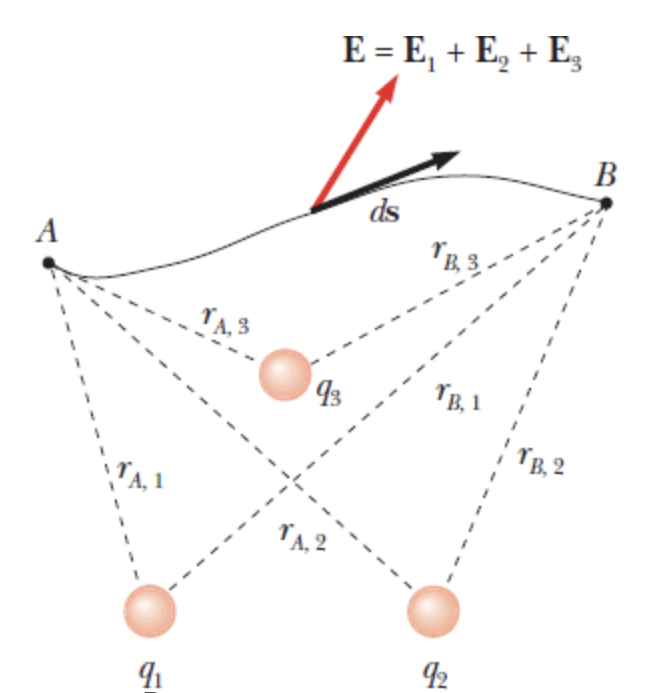
\includegraphics[width=0.45\linewidth]{figure/image4.png}
    \caption{Schema per il calcolo di $\int_A ^B \mathbf{E} \cdot d \mathbf{s}$ per il campo elettrostatico prodotto da un insieme di cariche}  
    \label{fig:calcolo_potenziale_n_cariche}
\end{figure}

\begin{equation*}
    \int_A ^B \mathbf{E} \cdot d \mathbf{s} = \int_A ^B (\sum_i \mathbf{E}_i) \cdot d \mathbf{s} = \sum_i \int_A ^B \mathbf{E}_i \cdot d \mathbf{s} = \sum_i \int_A ^B \frac{q_i}{4 \pi \varepsilon_0 r_i ^2} \mathbf{u}_i \cdot d \mathbf{s}
\end{equation*}

Ciascun integrale porta a un risultato tipo \ref{eq:differenza_di_potenziale} e quindi il campo elettrostatico delle $n$ cariche è conservativo, in particolare risulta che 

\begin{equation}
    V_B - V_A = (\sum_i \frac{q_i}{4 \pi \varepsilon_0 r_{B,i}} - \sum_i \frac{q_i}{4 \pi \varepsilon_0 r_{A,i}})
\end{equation}

E per la convenzione adottata risulta che il potenziale elettrostatico generato dal sistema di cariche nel punto $P(x,y,z)$, distante $r_i$ dalla carica $q_i$, è 

\begin{tcolorbox}[colback=yellow!10!white, colframe=orange!70!black, boxrule=0.8pt]
\begin{equation}
    V(x,y,z) = - \int_{\infty} ^P \mathbf{E} \cdot d \mathbf{s} = \sum_i \frac{q_i}{4\pi \varepsilon_0r_i}
    \label{eq:potenziale_per_più_cariche}
\end{equation}
\end{tcolorbox}

Il potenziale elettrostatico prodotto da un sistema discreto di cariche è uguale alla somma dei potenziali elettrostatici prodotti singolarmente dalle cariche.\\

Nel caso che le cariche siano distribuite in modo continuo basta sostituire nella \ref{eq:potenziale_per_più_cariche} alla sommatoria l'integrale di linea, di superficie o di volume.

\begin{tcolorbox}[colback=yellow!10!white, colframe=orange!70!black, boxrule=0.8pt]
\begin{equation}
    V(x,y,z) = \frac{1}{4\pi \varepsilon_0} \int _{\tau} \frac{\rho (r)}{r} d\tau
    \label{eq:potenziale_senza_condizione}
\end{equation}
\end{tcolorbox}

dove l'integrazione è estesa a \emph{tutte le cariche dell'universo}.

\newpage


\chapter{Legge di Gauss}
Consideriamo una superficie infinitesima $d \Sigma$ in una regione in cui è definito un campo $\mathbf{E}$ e orientiamola fissando il verso del versore della normale $\mathbf{u}_n$. 

Si definisce \mkeyword{flusso del campo $\mathbf{E}$}flusso del campo $\mathbf{E}$ attraverso la superficie $d\Sigma$ la quantità scalare

\begin{equation*}
    d\Phi(\mathbf{E}) = \mathbf{E} \cdot \mathbf{u}_n d\Sigma = E \cos(\theta) d \Sigma
    \label{eq:flusso_infinitesimale}
\end{equation*}

Il flusso attraverso una superficie finita $\Sigma$ si ottiene suddividendola in elementi infinitesimi di superficie $d \Sigma_i$ e sommando gli infiniti contenuti del flusso per ciascuna $i$.

\begin{figure} [h]
    \centering
    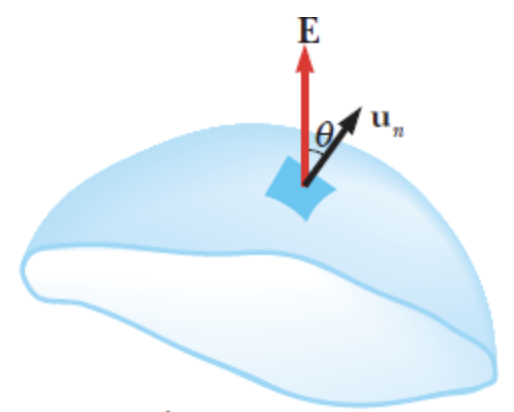
\includegraphics[width=0.4\linewidth]{figure/image6.png}
    \caption{Flusso del campo elettrico attraverso una superficie}
    \label{fig:chapter_3_1}
\end{figure}

Quindi 

\begin{equation}
    \Phi (\mathbf{E}) = \int_{\Sigma} \mathbf{E} \cdot \mathbf{u}_n d \Sigma  
\end{equation}

Se la superficie è chiusa, il flusso si scrive

\begin{equation}
    \Phi (\mathbf{E}) = \oint_{\Sigma} \mathbf{E} \cdot \mathbf{u}_n d \Sigma  
\end{equation}

Nella successiva sezione daremo la dimostrazione di una legge che si applica al campo elettrostatico, nota come \emph{legge} o teorema \emph{di Gauss}, evidenziando che questa vale \emph{se e solo se} la forza tra due cariche elementari è \emph{inversamente proporzionale al quadrato della distanza tra le stesse}.\\

La legge di Gauss \mkeyword{Legge di Gauss}afferma che il flusso del campo elettrostatico $\mathbf{E}$ prodotto da un sistema di cariche attraverso una superficie chiusa è uguale alla somma algebrica delle cariche elettriche contenute all'interno della superficie, divisa per $\varepsilon_0$

\begin{tcolorbox}[colback=yellow!10!white, colframe=orange!70!black, boxrule=0.8pt]
\begin{equation}
    \Phi(\mathbf{E}) = \oint_{\Sigma} \mathbf{E} \cdot \mathbf{u}_n \ d \Sigma = \frac{\sum_i q_i}{\varepsilon_0}
    \label{eq:Legge_di_Gauss}
\end{equation}
\end{tcolorbox}

\section{Dimostrazione della legge di Gauss}

Prima di iniziare la vera e propria dimostrazione andiamo a introdurre uno strumento che andrà a semplificare molto i calcoli, l'angolo solido.\\

Sia $d \Sigma$ un elemento di superficie, $\mathbf{u}_n$ la sua normale e $d \Sigma_0$ la sua proiezione ortogonale a $\mathbf{u}_r$, versore del raggio $r$ uscente da un punto di osservazione $O$.

\begin{figure}[h]
    \centering
    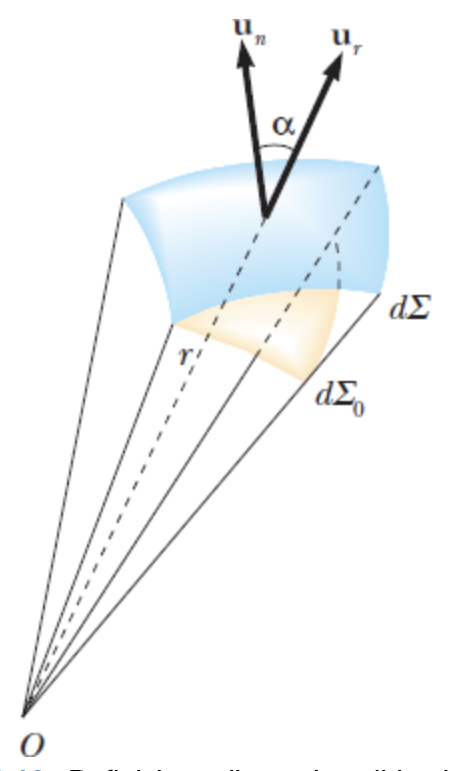
\includegraphics[width=0.32\linewidth]{figure/image7.png}
    \label{fig:chapter_3_2}
\end{figure}

Si definisce angolo solido \mkeyword{angolo solido} infinitesimo la quantità 

\begin{equation}
    d \Omega = \frac{d \Sigma \cos(\alpha)}{r^2} = \frac{d \Sigma_0}{r^2}
\end{equation}

Possiamo iniziare con la dimostrazione. Iniziamo prendendo in esame il campo elettrostatico prodotto da una carica puntiforme $q$, il flusso attraverso l'elemento di superficie orientata utilizzando la \ref{eq:flusso_infinitesimale}:

\begin{equation*}
    d \Phi(\mathbf{E}) = \frac{q}{4 \pi \varepsilon_0} \ \frac{\mathbf{u}_r \cdot \mathbf{u_n} \ d \Sigma}{r^2} = \frac{q}{4 \pi \varepsilon_0} \ \frac{d \Sigma_0}{r^2}
\end{equation*}

Per definizione $d \Sigma_0/r^2$ è l'angolo solido $d \Omega$ sotto cui è visto dalla carica $q$ il contorno di $d \Sigma$, per cui 

\begin{equation*}
    d \Phi (\mathbf{E}) = \frac{q}{4 \pi \varepsilon_0} d \Omega
\end{equation*}

Il \emph{flusso del campo elettrostatico $\mathbf{E}$ di una carica puntiforme $q$ dipende solo dall'angolo solido e non dalla superficie né dalla sua distanza dalla carica}.\\

Conviene osservare subito che la dipendenza del flusso dall'angolo solido \emph{conseguenza} del fatto che a denominatore dell'espressione del campo compare $r^2$: \emph{qualunque altra dipendenza funzionale non avrebbe portato alla \ref{eq:Legge_di_Gauss}}.\\
Il flusso attraverso una superficie finita è dato da 

\begin{equation*}
    \Phi(\mathbf{E}) = \int_{\Sigma} \mathbf{E} \cdot \mathbf{u}_n \ d \Sigma
 = \frac{q}{4 \pi \varepsilon_0} \int_{\Omega} d \Omega = \frac{q}{4 \pi \varepsilon_0} \Omega
\end{equation*}

Con $\Omega$ angolo solido sotto cui è visto il contorno della superficie $\Sigma$ dalla carica $q$.\\

Calcoliamo adesso il flusso di $\mathbf{E}$ attraverso una superficie chiusa, distinguendo due casi: quello in cui la \emph{carica $q$ è interna alla superficie} e il caso in cui è \emph{esterna}.\\

Se la carica è interna alla superficie tutti i contribuiti $\mathbf{E} \cdot \mathbf{u}_n \ d\Sigma$ si sommano in quanto hanno sempre lo stesso segno.

\begin{equation*}
    \Phi (\mathbf{E}) = \frac{q}{4\pi\varepsilon_0} \int_{\Omega} d\Omega = \frac{q}{4\pi\varepsilon_0} 4 \pi = \frac{q}{\varepsilon_0}
\end{equation*}

Se invece la superficie è chiusa consideriamo un cono elementare che sottende l'angolo solido $d \Omega$ e che stacca sulla superficie due elementi corrispondenti $d \Sigma_1$ e $d \Sigma_2$ di versori normali $\mathbf{u}_{n_1}$ e $\mathbf{u}_{n_2}$ rispettivamente; l'orientazione delle normali è tale che su $\mathbf{E}_1 \cdot \mathbf{u}_{n_1} d\Sigma_1 < 0$ e $\mathbf{E}_2 \cdot \mathbf{u}_{n_2} d\Sigma_2 > 0$.\\
I flussi infinitesimali attraverso le due superfici sono:

\begin{align*}
    d \Phi_1(\mathbf{E}) = \mathbf{E}_1 \cdot \mathbf{u}_{n_1} \ d \Sigma_1 = - \frac{q}{4 \pi \varepsilon_0} d\Omega \\ d\Phi_2 (\mathbf{E}) = \mathbf{E}_2 \cdot \mathbf{u}_{n_2} \ d \Sigma_1 = + \frac{q}{4 \pi \varepsilon_0} d\Omega \\ \implies d\Phi_1(\mathbf{E}) + d\Phi_2 (\mathbf{E}) = 0 
\end{align*}

\begin{figure}[h]
    \centering
    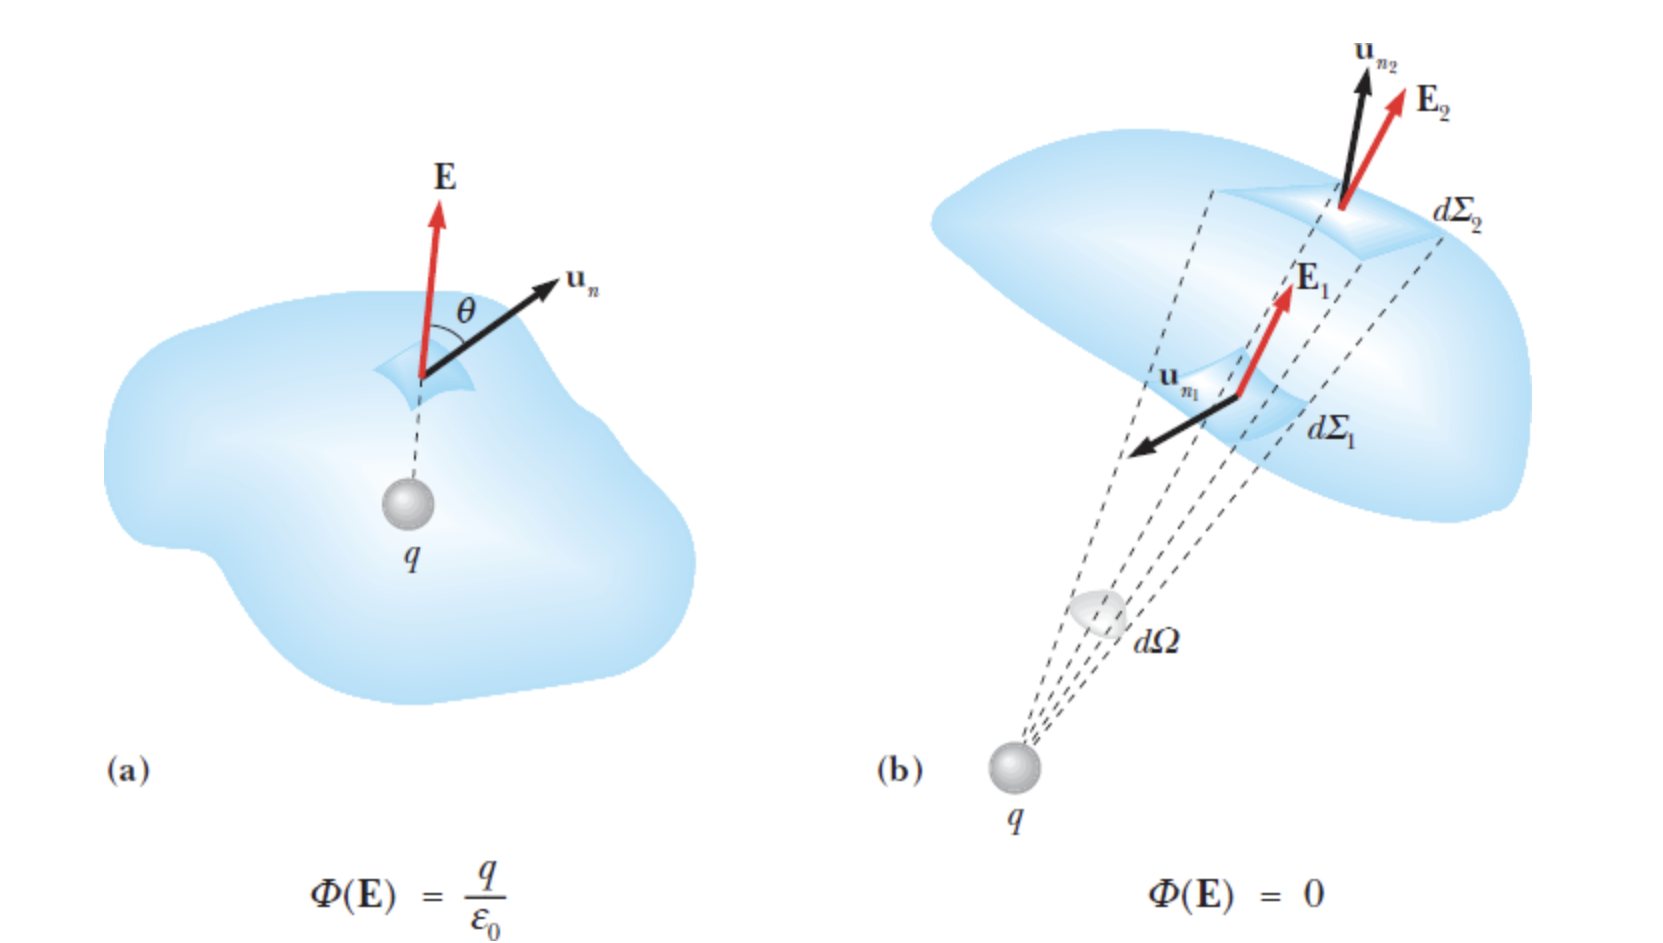
\includegraphics[width=01.0\linewidth]{figure/image8.png}
    \caption{Flusso del campo elettrostatico di una carica puntiforme attraverso una superficie chiusa quando la carica è all'interno della superficie (\textbf{a}) e quando è all'esterno (\textbf{b})}
    \label{fig:chapter_3_3}
\end{figure}

Integrando su tutta la superficie chiusa otteniamo infine 

\begin{equation*}
    \Phi(\mathbf{E}) = \oint_{\Sigma} \mathbf{E} \cdot \mathbf{u}_n \ d\Sigma = 0
\end{equation*}

Questi risultati si possono riassumere dicendo che il flusso attraverso una superficie chiusa del campo elettrostatico di una carica puntiforme $q$ vale $q/\varepsilon_0$ se la carica è interna alla superficie, vale zero se la carica è esterna. 

\newpage

Il risultato enunciato si estende al caso di più cariche puntiformi, attraverso il principio di sovrapposizione e la proprietà di additività dell'integrale.

\begin{equation*}
    \Phi(\mathbf{E}) = \oint_{\Sigma} \mathbf{E} \cdot \mathbf{u}_n  \ d \Sigma = \oint_{\Sigma} (\sum_i \mathbf{E}_i) \cdot \mathbf{u}_n  \ d \Sigma = \sum_i \oint_{\Sigma} \mathbf{E}_i \cdot \mathbf{u}_n  \ d \Sigma
\end{equation*}

Ciascuno integrale vale $q_i/ \varepsilon_0$ se la carica è contenuta all'interno della superficie e vale zero se è esterna. Pertanto abbiamo

\begin{equation*}
    \phi(\mathbf{E}) = \frac{(\sum_i q_i)_{\text{int}}}{\varepsilon_0}
\end{equation*}

Che è esattamente quello che volevamo dimostrare. \\

La legge di Gauss ha delle applicazioni e conseguenze importantissime e si consiglia al lettore di approfondire leggendo tale argomento in \cite{ElettromagnetismoeOnde}


\chapter{Relazioni locali}

Fino a questo momento abbiamo trovato tre equazioni integrali che caratterizzano il campo elettrostatico $\mathbf{E}$

\begin{equation*}
    V_B - V_A = - \int_A^B \mathbf{E} \cdot d \mathbf{s} \quad , \quad \oint \mathbf{E} \cdot d \mathbf{s} = 0 \quad , \quad \oint_{\Sigma} \mathbf{E} \cdot \mathbf{u}_n \ d \Sigma = \frac{q}{\varepsilon_0}
\end{equation*}

Tuttavia è possibile andare a trovare anche una relazione locale che esprime tale equazioni. \\

\' E importante sottolineare che una relazione è locale se, per sapere quanto vale una certa grandezza in un punto $P$, si deve conoscere solo il comportamento delle altre grandezze in quel punto (o in un intorno infinitesimo), non in punti lontani.

\section{Campo elettrostatico come gradiente del potenziale elettrostatico}

Consideriamo l'equazione integrale 

\begin{equation*}
    V_B - V_A = - \int_A^B \mathbf{E} \cdot d \mathbf{s}
\end{equation*}

Andiamo a dimostrare che esiste una relazione locale che permette, dalla conoscenza del potenziale elettrostatico in ogni punto della regione, di calcolare il campo elettrostatico in ogni punto della stessa regione. \\

In \emph{coordinate cartesiane}, per uno spostamento $d \mathbf{s} = dx \ \mathbf{u}_x + dy \ \mathbf{u}_y + dz \ \mathbf{u}_z$ che unisce due punti $A (x,y,z)$ e $B(x+dx, y+dy, z+dz)$ la variazione di potenziale elettrostatico è 

\begin{equation*}
    dV = V(x+dx, y+dy, z+dz) - V(x,y,z) = - \mathbf{E} \cdot d \mathbf{r} = - E_x \ dx - E_y \ dy - E_z \ dz 
\end{equation*}

D'altra parte, per il teorema del differenziale totale

\begin{equation*}
    dV = \frac{\partial V}{\partial x} \ dx + \frac{\partial V}{\partial y} \ dy + \frac{\partial V}{\partial z} \ dz
\end{equation*}

Dal confronto delle due espressioni si ricavano le uguaglianze

\begin{equation*}
    E_x = - \frac{\partial V}{\partial x} \quad, \quad E_y = - \frac{\partial V}{\partial y} \quad, \quad E_z = - \frac{\partial V}{\partial z} 
\end{equation*}

\newpage

Scritto in modo più sintetico 

\begin{tcolorbox}[colback=yellow!10!white, colframe=orange!70!black, boxrule=0.8pt]
\begin{equation}
    \mathbf{E} = - \nabla V
    \label{eq:Campoelettrostatico_come_gradiente}
\end{equation}
\end{tcolorbox}

Dove l'operatore \emph{nabla}, \mkeyword{nabla, coordinate cartesiane} in coordinate cartesiane, è definito come

\begin{equation}
    \mathbf{\nabla } = \frac{\partial}{\partial x} \mathbf{u}_x + \frac{\partial}{\partial y} \mathbf{u}_y + \frac{\partial}{\partial z} \mathbf{u}_z = \colvec{\frac{\partial}{\partial x} \\ \frac{\partial}{\partial y} \\ \frac{\partial}{\partial z}}
\end{equation}

Sostituendo il risultato ottenuto nella \ref{eq:differenza_di_potenziale}
si ottiene un teorema generale del calcolo vettoriale, noto come teorema del gradiente \mkeyword{teorema del gradiente}:

\begin{tcolorbox}[colback=yellow!10!white, colframe=orange!70!black, boxrule=0.8pt]
\begin{equation}
    V_B - V_A = \int_A^B \nabla V \cdot d \mathbf{s}
    \label{thrm:teorema_del_gradiente}
\end{equation}
\end{tcolorbox}

La variazione di una funzione scalare tra due punti $A$ e $B$ è data dall'integrale di linea del gradiente della funzione scalare lungo una qualunque linea che unisca $A$ e $B$. 



\subsection{Superfici equipotenziali}

\mkeyword{superfici equipotenziali}L'andamento di un potenziale elettrostatico è visualizzabile ricorrendo alle superfici equipotenziali definite come le superfici dello spazio tridimensionale nei cui punti il potenziale ha lo stesso valore. \\

Ricordando le proprietà di direzione e verso del gradiente, che ad ogni modo si deducono dalla \ref{thrm:teorema_del_gradiente},

\begin{equation*}
    dV = \nabla V \cdot d \mathbf{s} = - \mathbf{E} \cdot d \mathbf{s} 
\end{equation*}

abbiamo che per uno spostamento $d \mathbf{s}$ tangente a una superficie equipotenziale la variazione $dV$ è ovviamente nulla e quindi il gradiente è ortogonale in ogni punto alla superficie equipotenziale. \\
Inoltre si ha che il campo elettrostatico risulta in ogni punto perpendicolare alla superficie equipotenziale passante per quel punto e il suo verso indica il verso di crescita del potenziale elettrostatico e le superfici equipotenziali sono ortogonali alle linee di forza.



\newpage

\section{Rotore di un campo vettoriale e Teorema di Stokes}

Consideriamo un percorso rettangolare infinitesimo ABCD che giace sul piano \emph{yz} e ha i lati, lunghi $AB = dy$ e $BC = dz$ paralleli agli assi, vogliamo clacolare la circuitazione di un \emph{generico} campo vettoriale $\mathbf{E}$.

\begin{figure} [h]
    \centering
    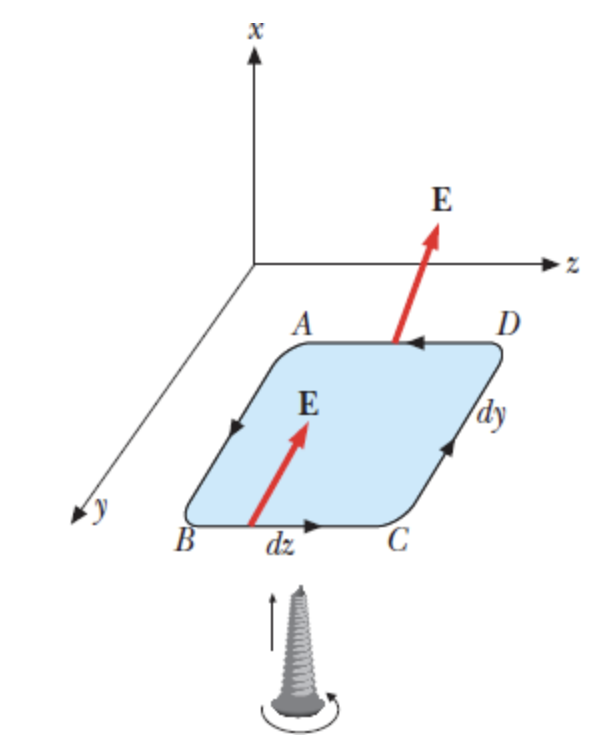
\includegraphics[width=0.5\linewidth]{figure/image2.png}
    \caption{Calcolo della circuitazione di un campo vettoriale $\mathbf{E}$}
    \label{fig:chapter_4_1}
\end{figure}

Il verso di percorrenza è dato dalla \emph{regola della vite destrorsa} \mkeyword{regola della vita destrorsa}, come si vede dal disegno, \emph{ruotando lungo il verso di percorrenza della vita destrorsa, la punta della vite indica il verso dell'asse x}. L'area vale $d \Sigma_x = dy \ dx$.

\begin{equation*}
    d \Gamma_x(\mathbf{E}) = \mathbf{E}(AB) \cdot \mathbf{AB} + \mathbf{E}(BC) \cdot \mathbf{BC} + \mathbf{E}(CD) \cdot \mathbf{CD} + \mathbf{E}(DA) \cdot \mathbf{DA}
\end{equation*}

Dato che $\mathbf{CD} = \mathbf{-AB}$ e $\mathbf{DA} = \mathbf{-BC}$ 

\begin{equation*}
    d \Gamma_x(\mathbf{E}) = [\mathbf{E}(AB) - \mathbf{E}(CD)] \cdot dy \ \mathbf{u}_y + [\mathbf{E}(BC) - \mathbf{E}(DA)] \cdot dz \ \mathbf{u}_z
\end{equation*}

Svolgendo i prodotti scalari e sostituendo le coordinate si ottiene 

\begin{equation*}
    d \Gamma_x(\mathbf{E}) = [E_y(z) - E_y(z + dz)] \cdot dy  + [E_z(y + dy) - E_z(y)] \cdot dz
\end{equation*}

Sviluppando in serie le differenze e fermandosi al primo ordine 

\begin{equation*}
    E_y(z + dz) - E_y(z) = \frac{\partial E_y}{\partial z} dz \quad , \quad E_z(y + dy) - E_z(y) = \frac{\partial E_z}{\partial y} dy
\end{equation*}

Pertanto 

\begin{equation*}
    d \Gamma_x(\mathbf{E}) = (\frac{\partial E_z}{\partial y} - \frac{\partial E_y}{\partial z} ) dy\ dz = (\frac{\partial E_z}{\partial y} - \frac{\partial E_y}{\partial z} ) d \Sigma_x
\end{equation*}

\newpage

Procendendo in modo analogo sui piani $xz$ e $xy$ si ottiene 

\begin{align*}
        d \Gamma_y(\mathbf{E}) = (\frac{\partial E_x}{\partial z} - \frac{\partial E_z}{\partial x} ) d \Sigma_y   \\  d \Gamma_z(\mathbf{E}) = (\frac{\partial E_y}{\partial x} - \frac{\partial E_x}{\partial y} ) d \Sigma_z
\end{align*}

Consideriamo adesso un punto nello spazio e una superficie $d \Sigma $ infinitesima alla quale associamo il vettore $d \Sigma \ \mathbf{u}_n$. Da cui 

\begin{equation*}
    d \Sigma \ \mathbf{u}_n = \colvec{d \Sigma_x \\ d \Sigma_y \\ d \Sigma_z}
\end{equation*}

La circuitazione $d \Gamma$ del vettore $\mathbf{E}$ lungo il contorno $d \Sigma$ è uguale alla somma delle circuitazioni $d \Gamma_x$, $d \Gamma_y$, $d \Gamma_z $, quindi 

\begin{equation}
    d\Gamma(\mathbf{E}) = (\frac{\partial E_z}{\partial y} - \frac{\partial E_y}{\partial z} ) d \Sigma_x + (\frac{\partial E_x}{\partial z} - \frac{\partial E_z}{\partial x} ) d \Sigma_y + (\frac{\partial E_y}{\partial x} - \frac{\partial E_x}{\partial y} ) d \Sigma_z
    \label{eq: circuitazione}
\end{equation}

Dato che il secondo membro dell'equazione ha la forma di un prodotto scalare tra $d \Sigma \mathbf{u}_n$ e un altro vettore, possiamo definire questo secondo vettore come rotore del campo vettoriale \mkeyword{rotore del campo vettoriale} come 

\begin{equation}
     \nabla \times \mathbf{E} = (\frac{\partial E_z}{\partial y} - \frac{\partial E_y}{\partial z} ) \mathbf{u}_x + (\frac{\partial E_x}{\partial z} - \frac{\partial E_z}{\partial x} ) \mathbf{u}_y + (\frac{\partial E_y}{\partial x} - \frac{\partial E_x}{\partial y} ) \mathbf{u}_z
\end{equation}

Che equivale a dire 

\begin{equation*}
     \nabla \times \mathbf{E} = \colvec{\frac{\partial E_z}{\partial y} - \frac{\partial E_y}{\partial z} \\ \frac{\partial E_x}{\partial z} - \frac{\partial E_z}{\partial x} \\ \frac{\partial E_y}{\partial x} - \frac{\partial E_x}{\partial y}}
\end{equation*}

In questo modo la \ref{eq: circuitazione} può essere scritta come 

\begin{equation}
    d \Gamma (\mathbf{E}) = (\nabla \times \mathbf{E}) \cdot d \Sigma \ \mathbf{u}_n
\end{equation}

Possiamo quindi affermare che la circuitazione di un campo vettoriale $\mathbf{E}$ lungo una linea infinitesima nell'intorno di un punto è uguale al flusso del rotore del campo vettoriale $\mathbf{E}$ attraverso un qualunque elemento di superficie $d \Sigma$ che abbia la linea come contorno. \\


Se si estende questo ragionamento \mkeyword{Teorema di Stokes} a un percorso finito si ottiene il Teorema di Stokes  \footnote{Un approfondimento a proposito si trova nell'appendice A in \cite{ElettromagnetismoeOnde}} 

\begin{tcolorbox}[colback=yellow!10!white, colframe=orange!70!black, boxrule=0.8pt]
\begin{equation}
    \oint_C \mathbf{E} \cdot d\mathbf{s} = \int_{\Sigma} (\nabla \times \mathbf{E}) \cdot d \Sigma \mathbf{u}_n
    \label{Teorema di Stokes}
\end{equation}
\end{tcolorbox}


La circuitazione di un campo vettoriale lungo una linea chiusa orientata $C$ è uguale al flusso del rotore del campo attraverso una qualunque superficie $\Sigma$ che abbia $C$ come contorno, orientata concordamente a $C$ con la regola della vite destrorsa. \\
Si nota che nella \ref{Teorema di Stokes} quello a primo membro è un integrale di linea, mentre quello a secondo membro è un integrale di superificie. 

\subsection{Campo vettoriale conservativo}

Se il campo vettoriale, \emph{come nel caso del campo elettrostatico $\mathbf{E}$}, è conservativo, vale 

\begin{equation*}
    \oint \mathbf{E} \cdot d \mathbf{s} = 0
\end{equation*}

perciò la circuitazione è nulla lungo una qualsiasi linea chiusa $\Gamma$, quindi, dovendo essere valida per ogni superficie $\Sigma$ che poggi su $\Gamma$, vale 

\begin{tcolorbox}[colback=yellow!10!white, colframe=orange!70!black, boxrule=0.8pt]
\begin{equation}
\nabla \times \mathbf{E} = 0 
\end{equation}
\end{tcolorbox}

Il campo elettrostatico è un campo il cui rotore è nullo, ovvero un campo irrotazionale.

\newpage

\section{Legge di Gauss in forma differenziale.\\ Divergenza di un campo vettoriale.}

La legge di Gauss nella forma \ref{eq:Legge_di_Gauss} è una legge integrale che lega il flusso il flusso del campo elettrostatico $\mathbf{E}$ attraverso una superficie chiusa a quelle sorgenti del campo che stanno all'interno delle superfici. \\

Dimostreremo adesso che tale legge può essere espressa in forma differenziale tramite una \emph{relazione locale} che lega le derivate del campo in un determinato punto con la denisità della carica $\rho$ in quel punto. \\

Consideriamo un parallelepidedo infinitesimo centrato in $P \equiv (x,y,z)$, con spigoli $dx,dy,dz$ paralleli agli assi e volume $d \tau = dx \ dy \ dz$, che contiene la carica $dq = \rho (x,y,z) d\tau$. 

\begin{figure} [h]
    \centering
    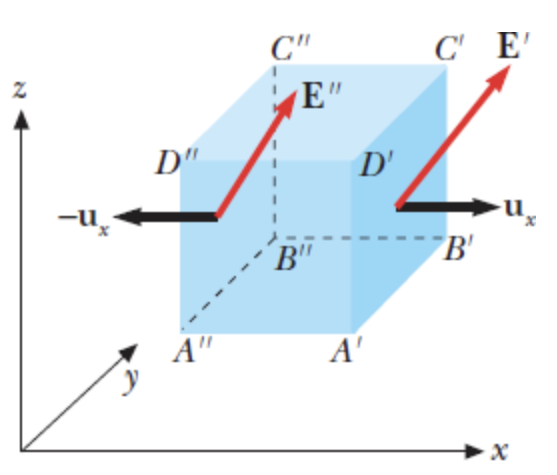
\includegraphics[width=0.5\linewidth]{figure/image11.png}
    \caption{Definizione di divergenza di un campo vettoriale}
    \label{fig:chapter_4_2}
\end{figure}

Il flusso del campo elettrostatico $\mathbf{E}$ attraverso la faccia $A'B'C'D'$, perpendicolare all'asse x, è dato da:

\begin{equation*}
    \mathbf{E}' \cdot \mathbf{u}_x \ dy \ dz = E_x ' \ dy \ dz
\end{equation*}

avendo indicato con $E_x'$ la componente di $\mathbf{E}' = \mathbf{E}\ (x + \frac{dx}{2}, y,z)$ lungo l'asse $x$. Analogamente il flusso attraverso la faccia $A''B''C''D''$ è 

\begin{equation*}
    \mathbf{E}'' \cdot (- \mathbf{u}_x) \ dy \ dz = -E_x '' \ dy \ dz
\end{equation*}

Dove $E_x '' $ è la componente di $\mathbf{E}'' = \mathbf{E}\ (x - \frac{dx}{2}, y,z)$ lungo l'asse $x$. Complessivamente 

\begin{equation*}
    (E'_x - E_x '') \ dy \ dz = \frac{\partial E_x}{\partial x} \ dx \ dy \ dz
\end{equation*}

Espressioni simili si hanno per le altre coppie di superficie e quindi il flusso attraverso tutta la superficie del parallelepipedo è:

\begin{equation*}
    d \Phi (\mathbf{E}) = \mathbf{E} \cdot \mathbf{u}_n \ d \Sigma  = \left ( \frac{\partial E_x}{\partial x} + \frac{\partial E_y}{\partial y} + \frac{\partial E_z}{\partial z} \right ) \ dx \ dy \ dz = \left ( \frac{\partial E_x}{\partial x} + \frac{\partial E_y}{\partial y} + \frac{\partial E_z}{\partial z} \right ) d \tau
\end{equation*}

Poiché, secondo la legge di Gauss \ref{eq:Legge_di_Gauss},

\begin{equation*}
    d \Phi (\mathbf{E}) = \frac{dq}{\varepsilon_0} = \rho (x,y,z) \frac{d \tau}{\varepsilon_0}
\end{equation*}

Quindi otteniamo la relazione locale che cercavamo:

\begin{equation}
    \frac{\partial E_x}{\partial x} + \frac{\partial E_y}{\partial y} + \frac{\partial E_z}{\partial z} = \frac{1}{\varepsilon_0} \rho (x,y,z)
\end{equation}

La combinazione di derivate a primo membro prende il nome di \mkeyword{divergenza del campo $\mathbf{E}$} divergenza del campo $\mathbf{E}$. \\
QUindi vale:

\begin{tcolorbox}[colback=yellow!10!white, colframe=orange!70!black, boxrule=0.8pt]
\begin{equation}
    \nabla \cdot \mathbf{E} = \frac{\rho}{\varepsilon_0}
    \label{eq:Gauss_forma_differenziale}
\end{equation}
\end{tcolorbox}

Il campo $\mathbf{E}$ ha divergenza diversa da zero solo nei punti in cui è diversa da zero la densità di carica. \\

Inoltre si vede facilmente che vale 

\begin{tcolorbox}[colback=yellow!10!white, colframe=orange!70!black, boxrule=0.8pt]
\begin{equation}
    d \Phi (\mathbf{E}) = \nabla \cdot \mathbf{E} \ d \tau
\end{equation}
\end{tcolorbox}

Considerato un volume infinitesimo $d \tau$ nell'intorno di un punto $P$ il flusso del campo vettoriale attraverso la superficie chiusa che delimita $d \tau$ è uguale al prodotto della divergenza del vettore per il volume $d \tau$ stesso. \\

Facendo il passaggio a un volume finito $\tau$ delimitato dalla superficie chiusa $\Sigma$, si ottiene un teorema \mkeyword{teorema della divergenza} generale del calcolo vettoriale noto come teorema della divergenza 

\begin{tcolorbox}[colback=yellow!10!white, colframe=orange!70!black, boxrule=0.8pt]
\begin{equation}
    \oint _{\Sigma} \mathbf{E} \cdot \mathbf{u}_n \ d \Sigma = \int_{\tau} \nabla \cdot \mathbf{E}\ d \tau
\end{equation}
\end{tcolorbox}

\subsection{Equazioni di Poisson e di Laplace}

Poiché nel campo elettrostatico $\mathbf{E}$ vale la \ref{eq:Campoelettrostatico_come_gradiente}, sostituendo nell'espressione \ref{eq:Gauss_forma_differenziale} si ottiene 

\begin{equation}
    \nabla \cdot \mathbf{E} = - \nabla \cdot \nabla V = -\nabla^2 V  = \frac{\rho}{\varepsilon_0}
\end{equation}

Operando in coordinate cartesiane si ottiene 

\begin{tcolorbox}[colback=yellow!10!white, colframe=orange!70!black, boxrule=0.8pt]
\begin{equation}
    \nabla ^2 V = \frac{\partial^2 V}{\partial x^2} + \frac{\partial^2 V}{\partial y^2} + \frac{\partial^2 V}{\partial z^2} = - \frac{\rho}{\varepsilon_0}
    \label{eq:equazione_di_Poisson}
\end{equation}
\end{tcolorbox}

Questa equazione differenziale che lega \mkeyword{Equazione di Poisson}il potenziale alla densità di carica è detta equazione di Poisson. \\

Nello spazio vuoto essa diventa

\begin{tcolorbox}[colback=yellow!10!white, colframe=orange!70!black, boxrule=0.8pt]
\begin{equation}
   \nabla ^2 V = \frac{\partial^2 V}{\partial x^2} + \frac{\partial^2 V}{\partial y^2} + \frac{\partial^2 V}{\partial z^2} = 0
\end{equation}
\end{tcolorbox}

ed \mkeyword{Equazione di Laplace} è detta equazione di Laplace.\\

L'operatore \mkeyword{laplaciano} $\nabla^2 = \nabla \cdot \nabla$, che in coordinate cartesiane si scrive 

\begin{equation*}
    \nabla^2 = \frac{\partial^2}{\partial x^2} + \frac{\partial^2}{\partial y^2} + \frac{\partial^2}{\partial z^2}
\end{equation*}

si chiama laplaciano. 


\chapter{Energia elettrostatica}

Analizziamo il significato dell'energia potenziale elettrostatica di un sistema di cariche. \\

Supponiamo, per semplicità, di considerare un sistema discreto di cariche. 

\begin{figure}[h]
    \centering
    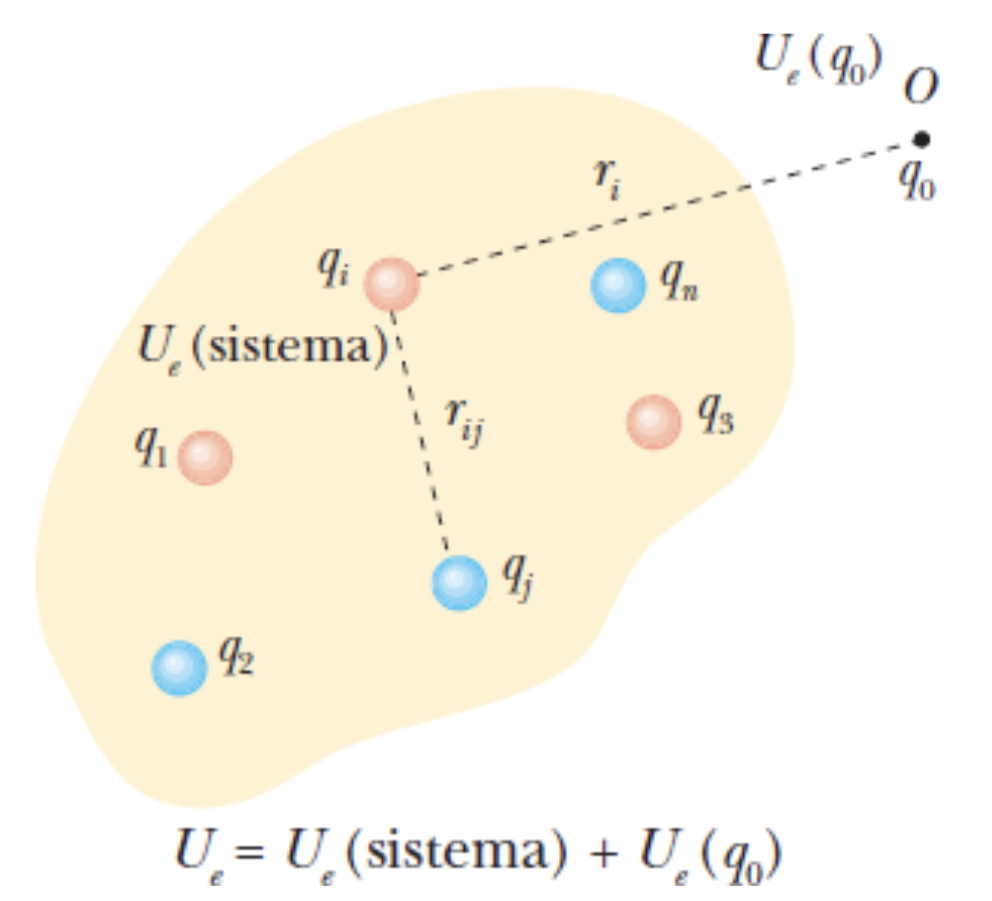
\includegraphics[width=0.47\linewidth]{figure/image5.png}
    \label{fig:chapter_5_1}
\end{figure}

Troviamo il lavoro necessario per creare questa distribuzione. Immaginiamo di portare le cariche una per una da una distanza infinita fino al suo punto nella distribuzione. Per la prima carica non ci sarà bisogno di compiere lavoro in quanto su di essa non agisce ancora nessun campo. Portando la seconda, sfruttando la \ref{eq:potenziale_per_più_cariche}, si dovrà fare un lavoro 

\begin{equation*}
    W_2 = \frac{1}{4 \pi \varepsilon_0} q_2 \left(\frac{q_1}{r_{12}}\right)
\end{equation*}

Dove $r_{12}$ è la distanza tra la prima e la seconda carica nella distribuzione. Portando la terza carica si ha 

\begin{equation*}
    W_3 = \frac{1}{4 \pi \varepsilon_0} q_3 \left( \frac{q_1}{r_{13}} + \frac{q_2}{r_{23}} \right)
\end{equation*}

In questo modo si capisce che per portare la carica j-esima si dovrà fare un lavoro 

\begin{equation}
    W_j = \frac{1}{4 \pi \varepsilon_0} q_j  \sum_{i=1} ^ {j-1}  \frac{q_i}{r_{ij}}
\end{equation}

Ma allora il lavoro totale sarà dato dalla somma di tutti questi lavori, quindi 

\begin{equation}
    W = \frac{1}{4 \pi \varepsilon_0} \sum_{i = 1} ^n \sum_{j>1}^n \frac{q_i  q_j}{r_{ij}}
\end{equation}

Dove la condizione $j>i$ è per non contare lo stesso paio di cariche due volte. Un modo migliore, allora, è quello di contare tutte le coppie di cariche due volte e poi dividere per due 

\begin{equation}
    W = \frac{1}{8 \pi \varepsilon_0} \sum_{i = 1} ^ {n} \sum_{j \neq i} ^n \frac{q_i q_j}{r_{ij}}
\end{equation}

Allora portando fuori dalla seconda sommatoria i termini che non dipendono da $j$, otteniamo 

\begin{equation}
    W = \frac{1}{2} \sum_{i = 1} ^n q_i \left( \sum_{j \neq i}^n \frac{1}{4 \pi \varepsilon_0} \frac{q_j}{r_{ij}} \right)
\end{equation}

Si nota che i termini in parentesi rappresentano il potenziale che agisce sulla carica j-esima una volta raggiunta la distribuzione, pertanto si ha che il lavoro totale necessario per ottenere la distribuzione è 

\begin{equation}
    W = \frac{1}{2} \sum_{i = 1}^n q_i V(\mathbf{r}_i)
\end{equation}

Ma questo lavoro rappresenta anche l'energia che il sistema accumula, quindi possiamo dire che l'energia elettrostatica del sistema è proprio 

\begin{tcolorbox}[colback=yellow!10!white, colframe=orange!70!black, boxrule=0.8pt]
\begin{equation}
    U_e = \frac{1}{2} \sum_{i \neq j} \frac{q_i q_j}{4 \pi \varepsilon_0 r_{ij}} = \frac{1}{2} \sum_{i = 1}^n q_i V(\mathbf{r}_i)
    \label{eq:energia_elettrostatica_discreto}
\end{equation}
\end{tcolorbox}

\section{Energia elettrostatica per una distribuzione continua}

Per una distribuzione continua di carica di densità di carica $\rho$ la \ref{eq:energia_elettrostatica_discreto} diventa

\begin{tcolorbox}[colback=yellow!10!white, colframe=orange!70!black, boxrule=0.8pt]
\begin{equation}
    U_e = \frac{1}{2} \int V dq = \frac{1}{2} \int_{\tau} \rho V \ d\tau
    \label{eq:energia_elettrostatica_continuo}
\end{equation}
\end{tcolorbox}

Tuttavia possiamo esprimere questo risultato in un'altra forma molto utile.\\
Sfruttando il teorema di Gauss in forma locale si ha 

\begin{equation*}
    \rho = \varepsilon_0 \nabla \cdot \mathbf{E} \implies U_e = \frac{\varepsilon_0}{2} \int_{\tau} (\nabla \cdot \mathbf{E}) V \ d \tau
\end{equation*}

Integrando per parti ed applicando il teorema della divergenza, otteniamo

\begin{equation}
    U_e = \frac{\varepsilon_0}{2} \left[ - \int_{\tau} \mathbf{E} \cdot (\nabla V) \ d \tau + \oint_{\Sigma} V \mathbf{E} \cdot \mathbf{u}_n \ d\Sigma \right]
\end{equation}

Tuttavia $\nabla V = - \mathbf{E}$, quindi 

\begin{equation}
    U_e = \frac{\varepsilon_0}{2} \left[  \int_{\tau} E^2 \ d \tau + \oint_{\Sigma} V \mathbf{E} \cdot \mathbf{u}_n \ d\Sigma \right]
\end{equation}

Ma su quale volume stiamo integrando adesso? Dalla \ref{eq:energia_elettrostatica_continuo} è chiaro che stiamo integrando sul volume della distribuzione, in realtà, però, andrebbe bene qualsiasi volume più grande contenente la distribuzione, in quanto tutto il volume in "eccesso" non darebbe alcun contributo all'integrale, dato che all'esterno della distribuzione $\rho = 0$. \\

Vediamo cosa succede quando andiamo a considerare volumi sempre più grandi. L'integrale contenente il termine $E^2$ può andare solo ad aumentare, questo implica che il secondo integrale deve andare a diminuire, per mantenere la quantità costante. \\

Si nota in questo modo che se andiamo a integrare in \emph{tutto lo spazio} allora si andrà ad annullare in contributo del secondo integrale e quindi avremo 

\begin{tcolorbox}[colback=yellow!10!white, colframe=orange!70!black, boxrule=0.8pt]
\begin{equation}
    U_e = \frac{\varepsilon_0}{2} \int E^2 \ d \tau
\end{equation}
\label{eq:energia_elettrostatica_campo}
\end{tcolorbox}

Dobbiamo fare sempre attenzione ad integrare su tutto lo spazio. 


\chapter{Dipolo elettrico}

Due \mkeyword{dipolo elettrico} cariche puntiformi $+ q$ e $-q$ mantenute a una distanza fissa $a$ costituiscono un dipolo elettrico. \\
\mkeyword{momento del dipolo}Si chiama momento del dipolo elettrico il vettore 

\begin{equation}
    \mathbf{p} = q  \mathbf{a}
\end{equation}

Dove $\mathbf{a}$ è orientato dalla carica negativa a quella positiva.

\begin{figure}[h]
    \centering
    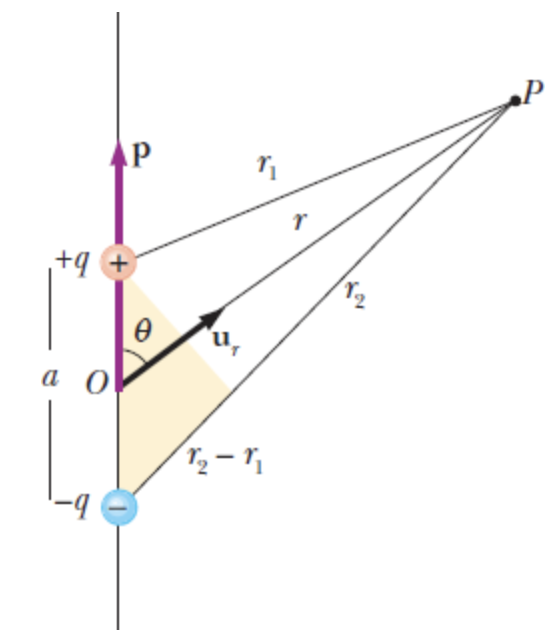
\includegraphics[width=0.4\linewidth]{figure/image12.png}
    \caption{Dipolo elettrico}
    \label{fig:chapter_6_1}
\end{figure}

Il potenziale elettrostatico del dipolo si trova con la \ref{eq:potenziale_per_più_cariche}:

\begin{equation*}
    V(P) = \frac{q}{4 \pi \varepsilon_0} (\frac{1}{r_1} - \frac{1}{r_2}) = \frac{q}{4 \pi \varepsilon_0}  \frac{r_2 - r_1}{r_1 r_2}
\end{equation*}

Se il punto $P$ è molto lontano dal dipolo, cioè $r \gg a $ (condizione detta approssimazione di dipolo), si può porre

\begin{equation}
    r_2 - r_1 = a \cos \theta \quad , \quad r_1 r_2 = r^2
\end{equation}

E quindi 

\begin{tcolorbox}[colback=yellow!10!white, colframe=orange!70!black, boxrule=0.8pt]
\begin{equation}
    V(P) = \frac{p \cos \theta}{4 \pi \varepsilon_0 r^2} = \frac{\mathbf{p} \cdot \mathbf{u}_r}{4 \pi \varepsilon_0 r^2}
    \label{eq:potenziale_dipolo}
\end{equation}
\end{tcolorbox}

Dalla formula si nota che l'unica grandezza caratteristica del dipolo è il momento $\mathbf{p}$ e non $q$ e $a$ separatamente: questo significa che da \emph{misure di potenziale elettrostatico possiamo ricavare informazioni du $\mathbf{p}$ ma non sulla costituzione del sistema}. \\
Geometricamente è spontanea la scelta delle coordinate polari sferiche aventi polo $O$ nel centro del dipolo. 

Andiamo a calcolare il campo elettrostatico con la \ref{eq:Campoelettrostatico_come_gradiente}:

\begin{align}
    E_r = - \frac{\partial V}{\partial r} = \frac{2 p \cos \theta}{4\pi \varepsilon_0 r^3}, \\ E_{\theta} =- \frac{1}{r} \frac{\partial V}{\partial \theta} = \frac{p \sin \theta}{4 \pi \varepsilon_0 r^3}\\
    E_{\varphi} = 0 \qquad \quad
\end{align}

Vettorialmente 

\begin{tcolorbox}[colback=yellow!10!white, colframe=orange!70!black, boxrule=0.8pt]
\begin{equation}
    \mathbf{E} = E_r \mathbf{u}_r + E_{\theta} \mathbf{u}_{\theta} = \frac{p}{4 \pi \varepsilon_0 r^3} (2 \cos \theta \ \mathbf{u}_r + \sin \theta \ \mathbf{u}_{\theta})
    \label{eq:componenti_campo_dipolo}
\end{equation}
\end{tcolorbox}

E il modulo vale 

\begin{equation}
    E = \frac{p}{4 \pi \varepsilon_0} \sqrt{3 \cos^2 \theta + 1}
\end{equation}

Tuttavia se si esprime il momento di dipolo in componenti polari:

\begin{equation}
    \mathbf{p} = p \cos \theta \ \mathbf{u}_r - p \sin \theta \ \mathbf{u}_{\theta} \implies p \sin \theta \ \mathbf{u}_{\theta} = p \cos \theta \ \mathbf{u}_r - \mathbf{p}
\end{equation}

Sostituendo nella \ref{eq:campo_dipolo} si ottiene 

\begin{tcolorbox}[colback=yellow!10!white, colframe=orange!70!black, boxrule=0.8pt]
\begin{equation}
    \mathbf{E} = \frac{1}{4 \pi \varepsilon_0 r^3} (3p \cos \theta \ \mathbf{u}_r - \mathbf{p}) = \frac{1}{4 \pi \varepsilon_0 r^3} \left [ 3(\mathbf{p} \cdot \mathbf{u}_r) \ \mathbf{u}_r - \mathbf{p}\right ]
\label{eq:campo_dipolo}
\end{equation}
\end{tcolorbox}

In particolare il secondo termine nel secondo membro rappresenta la componente antiparallela a $\mathbf{p}$.

\begin{figure}[h]
    \centering
    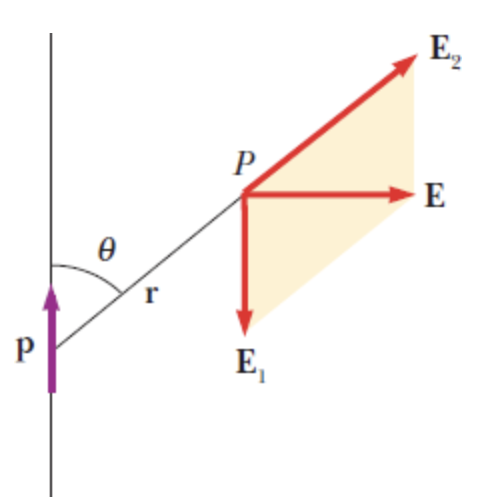
\includegraphics[width=0.4\linewidth]{figure/image13.png}
    \caption{Rappresentazione del un campo elettrostatico di un dipolo elettrico}
    \label{fig:campo_dipolo}
\end{figure}

\newpage

\section{Potenziale di una distribuzione di cariche nell'approssimazione di dipolo}

L'espressione \ref{eq:potenziale_dipolo} dedotta per il potenziale di due cariche puntiformi eguali e opposte può essere generalizzata per sistemi di cariche più complessi. \\

Consideriamo un sistema di cariche $q_i$ distribuite in una regione ristretta di dimesione massima $d$.

\begin{figure}[h]
    \centering
    \begin{subfigure}{0.48\textwidth}
        \centering
        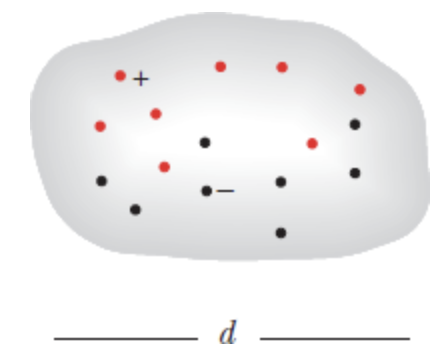
\includegraphics[width=0.7\linewidth]{figure/image14.png}
        \caption{Distribuzione di cariche }
        \label{fig:sub1}
    \end{subfigure}
    \hfill
    \begin{subfigure}{0.48\textwidth}
        \centering
        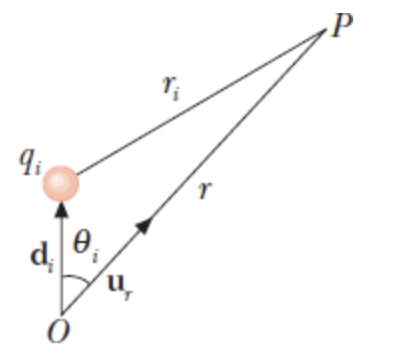
\includegraphics[width=0.7\linewidth]{figure/image15.png}
        \caption{Approssimazione di dipolo}
        \label{fig:sub2}
    \end{subfigure}
    %\caption{Confronto tra due campi elettrici}
    \label{fig:campi}
\end{figure}


Detto $O$ un qualsiasi punto interno alla regione, calcoliamo il potenziale elettrostatico in un punto $P$ a distanza $r$ da $O$ molto grande rispetto a $d \quad (r \gg d)$. Se $r_i$ è la distanza da $q_i$ a $P$

\begin{equation*}
    V = \frac{1}{4 \pi \varepsilon_0} \sum _i \frac{q_i}{r_i}
\end{equation*}

Chimando $\mathbf{d}_i$ il vettore che unisce $O$ alla carica $q_i$, abbiamo $\mathbf{d}_i + \mathbf{r}_i = \mathbf{r}$ e se vale $r \gg d_i$ possiamo scrivere

\begin{equation}
    r_i \approx r - d_i \cos \theta_i = r - \mathbf{d}_i \cdot \mathbf{u}_r
\end{equation}

Con $\mathbf{u}_r$ versore della direzione $OP$. Pertanto

\begin{equation}
    \frac{1}{r_i} \approx \frac{1}{r -\mathbf{d}_i \cdot \mathbf{u}_r} = \frac{r + \mathbf{d}_i \cdot \mathbf{u}_r}{r^2 - (\mathbf{d}_i \cdot \mathbf{u}_r)^2} \approx \frac{r + \mathbf{d}_i \cdot \mathbf{u}_r}{r^2 }
\end{equation}

Sostituendo nel potenziale 

\begin{equation}
    V \approx \frac{1}{4 \pi \varepsilon_0} \frac{\sum_i q_i (r + \mathbf{d}_i \cdot \mathbf{u}_r)}{r^2} =\frac{Q}{4 \pi \varepsilon_0 r} + \frac{(\sum_i q_i \mathbf{d}_i ) \cdot \mathbf{u}_r}{4 \pi \varepsilon_0 r^2}
\end{equation}

Definiamo il vettore \mkeyword{monento di dipolo di un sistema }

\begin{equation}
    \mathbf{p} = \sum_i q_i \ \mathbf{d} _i
\end{equation}

detto momento di dipolo elettrico del sistema rispetto al punto $O$ e quindi vale 

\begin{tcolorbox}[colback=yellow!10!white, colframe=orange!70!black, boxrule=0.8pt]
\begin{equation}
    V \approx \frac{Q}{4 \pi \varepsilon_0 r} + \frac{\mathbf{p} \cdot \mathbf{u}_r}{4 \pi \varepsilon_0 r^2} = V_0 + V_{\text{dip}}
\end{equation}
\end{tcolorbox}

\newpage

Il primo termine \mkeyword{monopolo} rappresenta il potenziale elettrostatico generato da una carica, eguale alla carica totale del sistema, posta nel punto $O$ e si chiama termine monopolo. Il secondo, formalmente uguale a \ref{eq:potenziale_dipolo}, si chiama termine di dipolo. \mkeyword{dipolo}\\

Se la $Q$ è diversa da zero il termine di monopolo è preponderante, infatti scrivendo 

\begin{equation*}
    \mathbf{p} = \sum_i q_i \mathbf{d}_i \approx Q \ \mathbf{d}
\end{equation*}

dove il modulo di $\mathbf{d}$ non è molto diverso dai moduli dei vari $\mathbf{d}_i$, abbiamo

\begin{equation*}
    \frac{V_{\text{dip}}}{V_0} = \frac{\mathbf{p} \cdot \mathbf{u}_r}{r Q} \approx \frac{Q d}{r Q} = \frac{d}{r} \ll 1
\end{equation*}

Se invece il sistema è neutro $(Q = 0)$, il termine di monopolo è nullo e il potenziale in $P$ è \emph{dato solo dal termine di dipolo}.\\

\' E possibile andare a schematizzare un sistema neutro pensandolo come due cariche $+ Q$ e $-Q$ poste a una certa distanza. \\

Per un sistema di $n$ cariche di un segno e $n$ cariche eguali ma di segno opposto possiamo scrivere

\begin{equation}
    \mathbf{p} = \sum_i q_i \mathbf{d}_i ^{(+)} - \sum_i q_i \mathbf{d}_i ^{(-)} = Q \ \mathbf{d}_1 - Q \ \mathbf{d}_2
\end{equation}

Quindi l'esistenza di un momento di dipolo in una distribuzione di cariche è legata all'esistenza di un' \emph{asimmetria}.\\

Quando $\mathbf{p} = 0$ il dipolo \mkeyword{termini di multipolo} non è sufficiente per il calcolo del potenziale, occorre introdurre nuovi termini che prendono il nome di termini di multipolo. 

\newpage

\section{Forza su un dipolo elettrico}

Consideriamo un dipolo elettrico avente centro in $O \equiv (x,y,z)$  e formato da una carica $-q$ posta in $P_1 \equiv (x - \frac{a_x}{2}, y - \frac{a_y}{2}, z - \frac{a_z}{2} )$ e in $P_2 \equiv (x + \frac{a_x}{2}, y + \frac{a_y}{2}, z + \frac{a_z}{2} )$; il vettore $\mathbf{a} = a_x \mathbf{u}_x + a_y \mathbf{u}_y + a_z \mathbf{u}_z$ congiunge $P_1$ e $P_2$ e il momento di dipolo è $\mathbf{p} = q \ \mathbf{a}$. 

\begin{figure}[h]
    \centering
    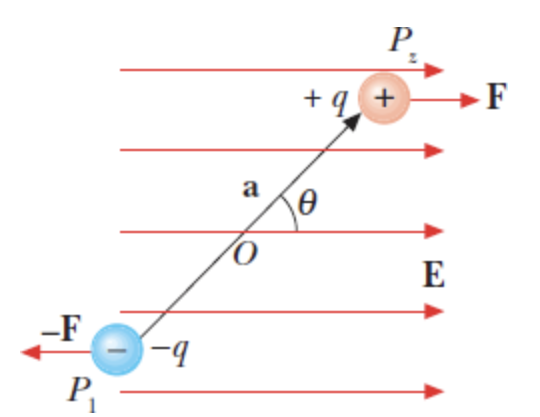
\includegraphics[width=0.4\linewidth]{figure/image16.png}
    \caption{Dipolo elettrico in un campo elettrostatico}
    \label{fig:dipolo_campo_elettrostatico}
\end{figure}

Se il dipolo si trova in un campo elettrostatic $\mathbf{E}$, la sua energia potenziale risulta essere

\begin{equation*}
U_e = q V(P_2) - q V(P_1) = q  [V(P_2) - V(P_1)]
\end{equation*}

Se la distanza $a$ è piccola (cosa che accade spesso nei dipoli), possiamo andare ad applicare il teorema del differenziale totale e scrivere

\begin{tcolorbox}[colback=yellow!10!white, colframe=orange!70!black, boxrule=0.8pt]
\begin{equation}
    U_e \approx q \ a_x \ \frac{\partial V}{\partial x} + q \ a_y \ \frac{\partial V}{\partial y}  + q \ a_z \ \frac{\partial V}{\partial z}  = \mathbf{p} \cdot \nabla V = - \mathbf{p \cdot \mathbf{E}} = - p \cos \theta \ E
    \label{eq:energia_potenziale_dipolo}
\end{equation}
\end{tcolorbox}

Dove \emph{le derivate parziali sono calcolate nel centro del dipolo}

\subsection{Campo elettrostatico uniforme}

Supponiamo che il campo elettrostatico in cui è immerso il dipolo sia uniforme, allora le forze sulle cariche $\mathbf{F}_1 = - q \ \mathbf{E}$, $\mathbf{F}_2 = q \ \mathbf{E}$, costituiscono una \emph{coppia} e quindi hanno risultante nulla.\\

Tuttavia il \emph{momento meccanico è diverso da zero}. Facendo ruotare il dipolo di un angolo $\theta$ rispetto alla posizione di equilibrio stabile, il dipolo risente di un momento delle forze $\mathbf{M}$ rispetto al centro del dipolo

\begin{equation}
    \mathbf{M} = \mathbf{r}_1 \times \mathbf{F}_1 + \mathbf{r}_2 \times \mathbf{F}_2 = (\mathbf{r}_2 - \mathbf{r}_1) \times q \ \mathbf{E} = q \ \mathbf{a} \times \mathbf{E} = \mathbf{p} \times \mathbf{E}
\end{equation}

Quindi vale 

\begin{tcolorbox}[colback=yellow!10!white, colframe=orange!70!black, boxrule=0.8pt]
\begin{equation}
    \mathbf{M} =\mathbf{p} \times \mathbf{E} =  - p \sin \theta \  E \  \mathbf{u}_z = - \frac{\partial U_e}{\partial \theta} \mathbf{u}_z
\end{equation}
\end{tcolorbox}

\subsection{Campo elettrostatico non uniforme}

Supponiamo, adesso, che il dipolo sia immerso in un campo elettrostatico non uniforme, in questo caso, oltre al momento $\mathbf{M}$, agisce una forza risultante $\mathbf{F}$, poiché le forze sulle due cairche $-q$ e $+q$ sono ora diverse in quanto diverso è il valore del campo elettrostatico nelle due posizioni. 

\begin{equation*}
    \mathbf{F}_1 = -q \ \mathbf{E}_1 \quad , \quad \mathbf{F}_2 = q \ \mathbf{E}_2 = q (\mathbf{E}_ + \frac{\partial \mathbf{E}}{\partial x} a_x  + \frac{\partial \mathbf{E}}{\partial y} a_y  + \frac{\partial \mathbf{E}}{\partial z} a_z )
\end{equation*}

Dove abbiamo sfruttato il teorema del differenziale totale. 

\begin{figure} [h]
    \centering
    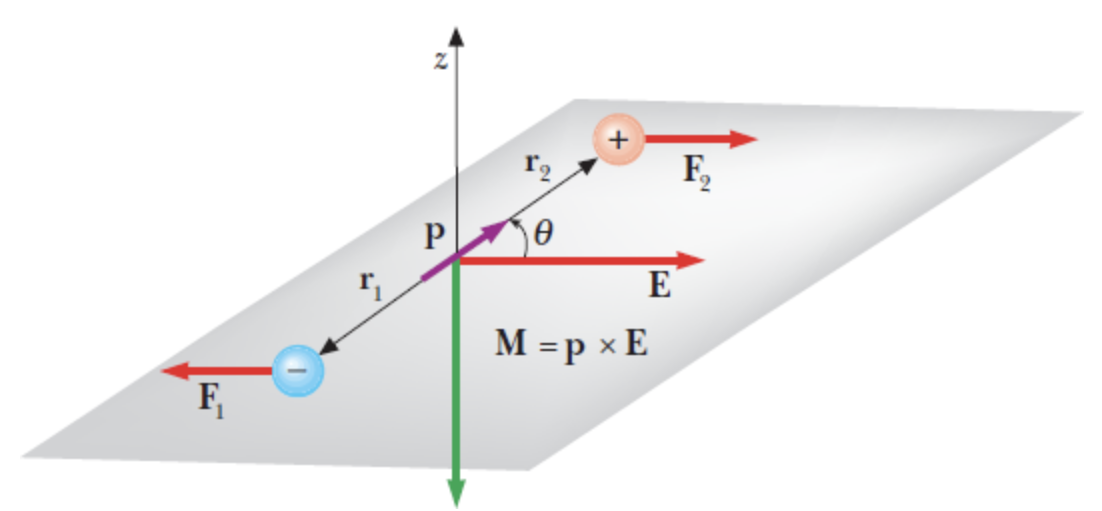
\includegraphics[width=0.6\linewidth]{figure/image17.png}
    \caption{Dipolo in un campo elettrostatico non uniforme}
    \label{fig:dipolo_campo_non_uniforme}
\end{figure}

La forza risultante è 

\begin{equation*}
    \mathbf{F} = \mathbf{F}_1 + \mathbf{F}_2 = q \ \mathbf{E}_2 = q \ a_x   \frac{\partial \mathbf{E}}{\partial x} + q \ a_y \frac{\partial \mathbf{E}}{\partial y}  + q \ a_z \frac{\partial \mathbf{E}}{\partial z}  
\end{equation*}

Ovvero 

\begin{tcolorbox}[colback=yellow!10!white, colframe=orange!70!black, boxrule=0.8pt]
\begin{equation}
    F = p_x \frac{\partial \mathbf{E}}{\partial x} + p_y \frac{\partial \mathbf{E}}{\partial y} + p_z \frac{\partial \mathbf{E}}{\partial z} = (\mathbf{p} \cdot \nabla) \ \mathbf{E}
\end{equation}
\end{tcolorbox}

\subsection{interazione tra dipoli}

Due dipoli elettrici di momenti elettrici $\mathbf{p}_1$ e $\mathbf{p}_2$, posti a distanza $r$ tra di loro, interagiscono in quanto ciascuno è sottoposto al campo elettrostatico dell'altro. 

\begin{figure}[h]
    \centering
    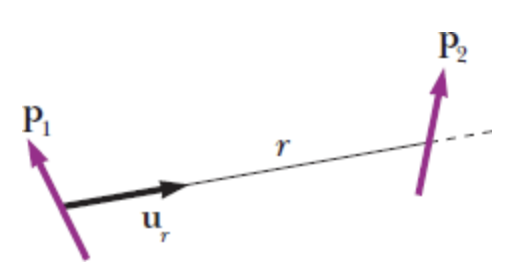
\includegraphics[width=0.4\linewidth]{figure/image18.png}
    \caption{Interazione tra dipoli}
    \label{fig:interazione_dipoli}
\end{figure}

Riprendendo la \ref{eq:potenziale_dipolo} e la \ref{eq:campo_dipolo}, si ottiene che il potenziale del secondo dipolo è 

\begin{equation}
    U_{e,2} = - \mathbf{p}_2 \cdot \mathbf{E}_1 = \frac{1}{4 \pi \varepsilon_0 r^3} [\mathbf{p}_1 \cdot \mathbf{p_2} - 3(\mathbf{p}_1 \cdot \mathbf{u}_r)(\mathbf{p}_2 \cdot \mathbf{u}_r) ]
\end{equation}

\newpage

Dove $\mathbf{u}_r$ è il versore della direnzione che va dal primo al secondo dipolo. Si vede che l'energia potenziale è simmetrica rispetto allo scambio di 1 e 2, quindi $U_{e,1} = U_{e,2}$. \\

La forza subita dal secondo dipolo è 

\begin{equation}
    \mathbf{F}_2 = - \nabla U_e 
\end{equation}

Si nota che la componente $r$ (supponendo di essere in coordinate sferiche) della forza è proporzionale a $1/r^4$

\begin{equation*}
    F_r  \propto \frac{1}{r^4}
\end{equation*}

quindi l'interazione decresce molto velocemente con la distanza.


\chapter{Conduttori}

Iniziamo dando una definizione di conduttore ed elencando alcune sue proprietà. \\

Un conduttore elettrico \mkeyword{conduttore elettrico} è un materiale in cui le cariche elettriche possono muoversi liberamente quando vengono sottoposte a un campo elettrico. Un conduttore \emph{perfetto} dovrebbe contenere un numero illimitato di cariche libere, questo tipo di conduttore, tuttavia, non esiste,  ma i metalli ci vanno molto vicino. \\

Da questa definizione è possibile intuire le seguenti proprietà di un conduttore. 

\begin{enumerate}
    \item \emph{$\mathbf{E} = 0$ all'interno di un conduttore in condizioni elettrostatiche.}\\ 

Questo perché se ci fosse un qualsiasi campo allora le cariche all'interno si muoverebbero e quindi non saremmo in condizioni elettrostatiche. \\

Vediamo cosa accade più nel dettaglio. \\
Supponiamo di mettere un conduttore in un campo elettrostatico esterno $\mathbf{E}_0$. Inizialmente il campo sposterà tutte le cariche positive libere nel verso del campo e quelle negative nel verso opposto. \footnote{In pratica, sono le cariche negative – gli elettroni – a muoversi, ma
quando si allontanano, il lato destro rimane con una carica positiva netta – i nuclei stazionari – quindi non importa quali cariche si muovano; l'effetto è lo stesso} \\
Quando arrivano al bordo del materiale, le cariche si accumulano generando una distribuzione superficiale di carica producendo così un campo proprio,
$\mathbf{E}_1$, che, come si può vedere dalla figura, è nella direzione opposta a $\mathbf{E}_0$. 

\begin{figure} [h]
    \centering
    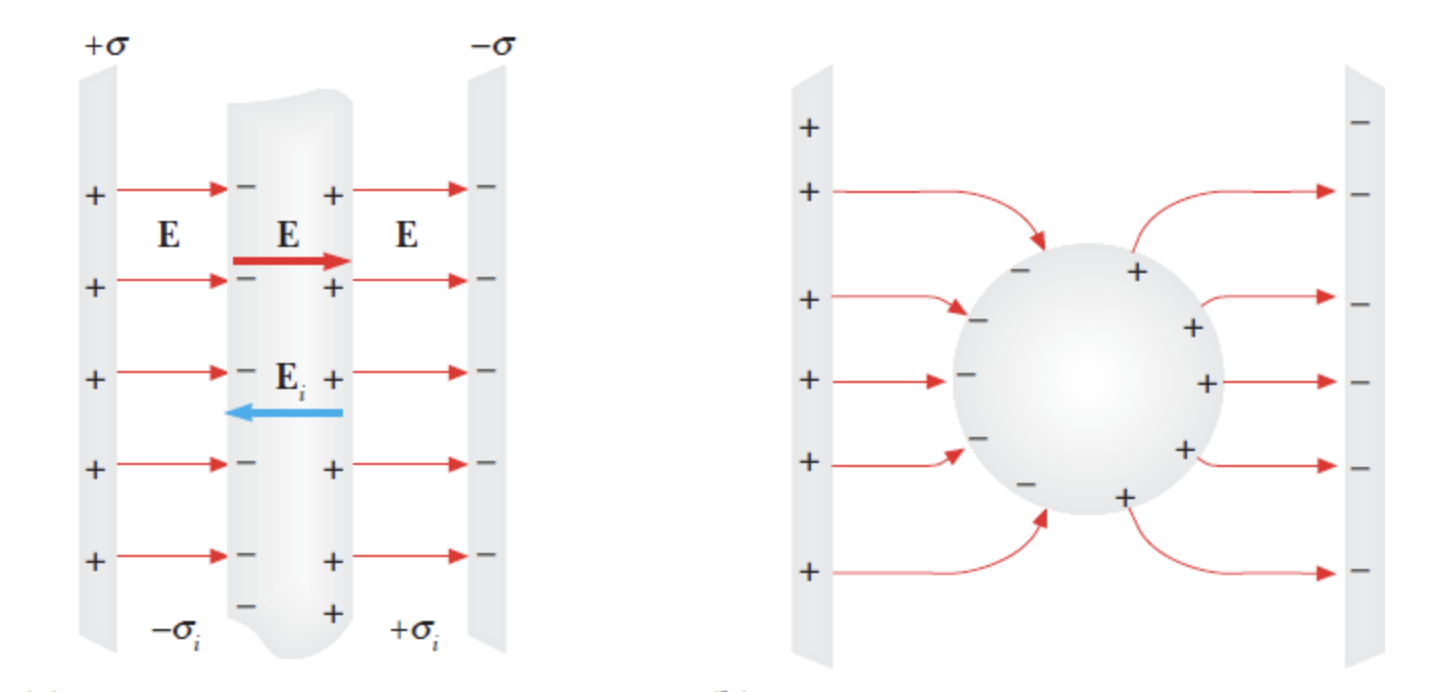
\includegraphics[width=0.8\linewidth]{figure/image30.png}
    \label{fig:chapter_7_1}
\end{figure}

Questo è il punto cruciale, perché significa che il campo delle cariche indotte tende ad annullare il campo originale. La carica continuerà a fluire finché questo annullamento non sarà completo,
e il campo risultante all'interno del conduttore sarà esattamente zero. 

\newpage

\item \emph{$\rho = 0$ all'interno del conduttore in condizioni stazionarie}. \\

Questo deriva dalle legge di Gauss in forma locale: $\nabla \cdot \mathbf{E} = \rho / \varepsilon_0$ ma se il campo è nullo all'interno allora lo sarà anche $\rho$. \\

\item \emph{I conduttori sono equipotenziali.} \\

Dati due qualsiasi punti $\mathbf{P}$ e $\mathbf{Q}$ dentro o sulla superficie del conduttore 

\begin{equation*}
    V(\mathbf{P}) - V (\mathbf{Q}) = \int_{\mathbf{P}} ^{\mathbf{Q}} \mathbf{E} \cdot d \mathbf{s} = 0 \implies V(\mathbf{P}) = V(\mathbf{Q})
\end{equation*}

\item \emph{$\mathbf{E}$ è ortogonale alla superficie e solo esterno.}\\

Dato che la superficie è equipotenziale il campo dovrà essere perpendicolare a essa e dato che all'interno deve essere nullo potrà avere componente non nulla solo all'esterno. \\

Il valore di $\mathbf{E}$ in un punto esterno molto vicino alla superficie di un conduttore si ricava applicando la legge di Gauss a un cilindro retto infinitesimo di basi $d \Sigma$ e superficie laterale di area trascurabile rispetto a $d \Sigma$, con una base contenuta all'interno del conduttore e l'altra in prossimità immediata del conduttore all'esterno. 
La carica contenuta all'interno della scatola cilindrica è $\sigma \ d\Sigma$ 

\begin{figure} [h]
    \centering
    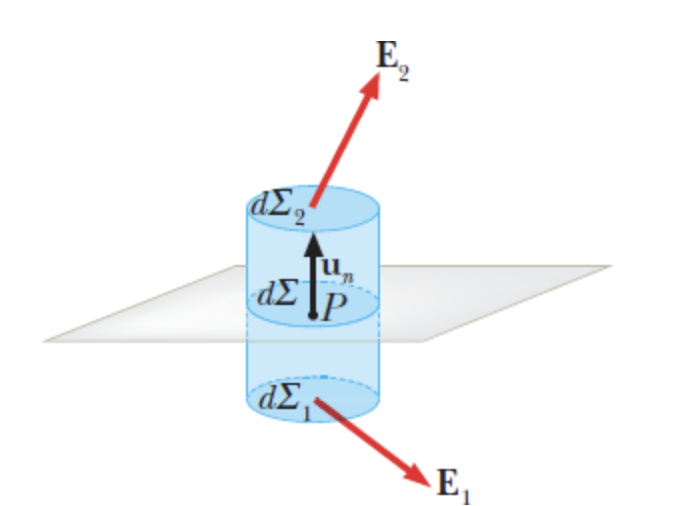
\includegraphics[width=0.5\linewidth]{figure/image31.png}
    \label{fig:chapter_7_2}
\end{figure}

allora 

\begin{equation*}
    \mathbf{E}_1 \cdot \mathbf{u}_1 \ d \Sigma + \mathbf{E}_2 \cdot \mathbf{u}_2 \ d \Sigma = (E_{2n} - E_{1n}) \ d \Sigma = \frac{\sigma \ d\Sigma}{\varepsilon_0}
\end{equation*}

Quindi si trova la relazione locale, \emph{del tutto generale}:

\begin{tcolorbox}[colback=yellow!10!white, colframe=orange!70!black, boxrule=0.8pt]
\begin{equation}
    E_{2n} - E_{1n} = \frac{\sigma}{\varepsilon_0}
\end{equation}
\end{tcolorbox}

Dato che siamo nel caso di un conduttore, $E_{1n} = 0$ in quanto interno, allora \emph{nel caso di un conduttore}

\begin{tcolorbox}[colback=yellow!10!white, colframe=orange!70!black, boxrule=0.8pt]
\begin{equation}
    \mathbf{E} = \frac{\sigma}{\varepsilon} \mathbf{u}_n 
\end{equation}
\end{tcolorbox}

\end{enumerate}

\section{Capacità di un conduttore isolato}

Supponiamo di considerare un conduttore isolato nello spazio con una distribuzione di carica superficiale $\sigma$

\begin{figure} [h]
    \centering
    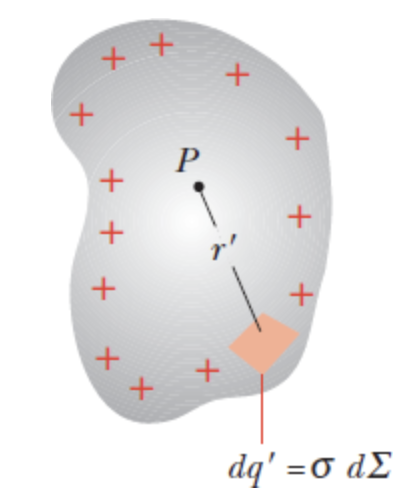
\includegraphics[width=0.30\linewidth]{figure/image32.png}
    \label{fig:chapter_7_3}
\end{figure}

allora la carica totale sarà 

\begin{equation*}
    q = \oint_{\Sigma} \sigma(x',y',z') d \Sigma
\end{equation*}

Il potenziale elettrostatico in un punto $\mathbf{P}$ qualsiasi del conduttore è dato dalla \ref{eq:potenziale_senza_condizione}

\begin{equation*}
    V = \frac{1}{4 \pi \varepsilon_0} \oint_{\Sigma} \frac{\sigma(x',y',z') d \Sigma}{r'}
\end{equation*}

Se la carica del conduttore viene portata al valore $q' = mq$ anche la densità varia localmente dello stesso fattore, $\sigma' = m \sigma$ e pure il potenziale elettrostatico del conduttore viene moltiplicato per $m$. \\

Da tali conseguenze si può dedurre che in un conduttore isolato il rapporto tra la carica elettrica e il \mkeyword{capacità del conduttore} potenziale elettrostatico non varia al variare della carica del conduttore, e tale rapporto si chiama  capacità del conduttore isolato:

\begin{tcolorbox}[colback=yellow!10!white, colframe=orange!70!black, boxrule=0.8pt]
\begin{equation}
    C = \frac{q}{V}
\end{equation}
\end{tcolorbox}

Si trova che essa dipende dalla forma e dalle dimensioni del conduttore e dal mezzo che lo circonda, in questo caso il vuoto. \\

L'unità di misura della capacità è il coulomb/volt, che prende il nome di \emph{farad}, \mkeyword{farad} simbolo $F$.

\newpage

\section{Conduttori cavi}

Consideriamo un conduttore carico che abbia nel suo interno una cavità all'interno della quale non ci siano cariche elettriche 

\begin{figure} [h]
    \centering
    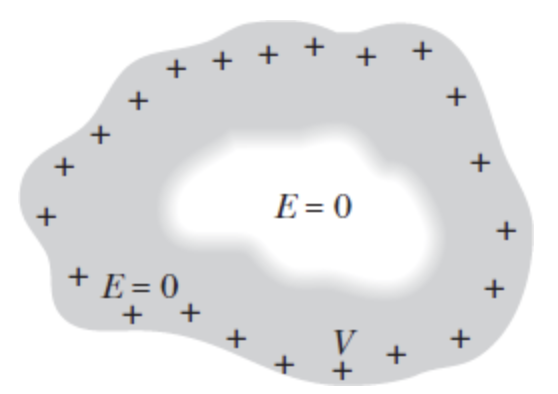
\includegraphics[width=0.4\linewidth]{figure/image33.png}
    \label{fig:chapter_7_4}
\end{figure}

Nella massa del conduttore il campo elettrostatico è nullo e pertanto il flusso è nullo è nullo attraverso qualsiasi superficie chiusa che racchiuda la cavità: segue, per la legge di Gauss, che all'interno della superficie non ci sono cariche e quindi \emph{sulle pareti della cavità la carica è nulla}.\\

Non è nemmeno possibile che sulle pareti ci sia una separazione della carica in $+q$ e $-q$ in quanto il campo elettrico è conservativo. Quindi si ha che \emph{sulle pareti della cavità non possono esserci cariche elettriche}.

\subsection{Gabbia di Faraday}

Consideriamo adesso un conduttore $C_2$ cavo, isolato e privo di carica, contenente un altro conduttore $C_1$ carico, isolato da $C_2$.

\begin{figure} [h]
    \centering
    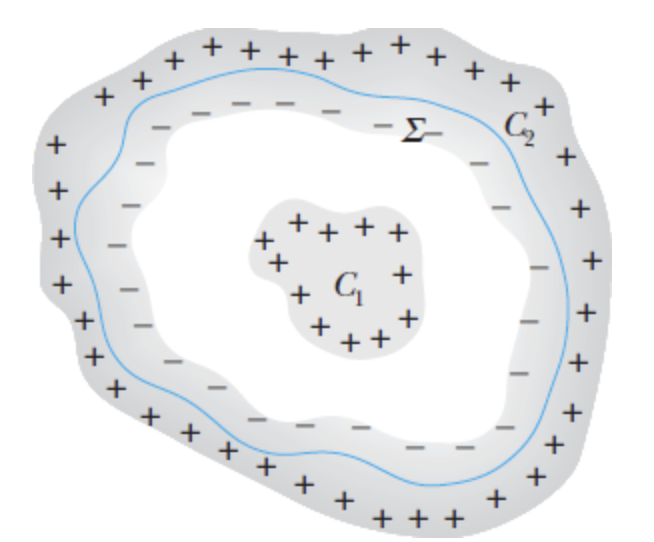
\includegraphics[width=0.4\linewidth]{figure/image34.png}
    \label{fig:chapter_7_5}
\end{figure}

In condizioni di equilibrio, se $C_1$ ha sulla sua superficie esterna una carica $q$, una carica $-q$ risulta distribuita sulla superficie interna e una carica $q$ sulla superficie esterna di $C_2$.\\

Tale fatto si spiega subito con la legge di Gauss: attraverso una superficie chiusa $\Sigma$ interna a $C_2$ e contenente la cavità il flusso di $\mathbf{E}$ è nullo in quanto è nullo il campo stesso; di conseguenza, all'interno di $\Sigma$ non c'è carica netta e se $C_1$ porta la carica $q$, sulla superficie interna di $C_2$ deve necessariamente comparire una carica $-q$. Inoltre essendo $C_2$ neutro, la distribuzione di una carica complessiva $-q$ sulla superficie interna comporta la comparsa di una carica complessiva $+q$ distribuita sulla superficie esterna.\\ 

Siamo di fronte a un fenomeno di induzione che in questo caso, essendo la carica $q$ completamente contenuta all'interno di una \mkeyword{induzione completa} cavità chiusa, si chiama induzione completa: tutte le linee di forza che partono da $C_1$ terminano su $C_2$. Dalla superficie esterna di $C_2$ partono altre linee di forza, il cui andamento in prossimità del conduttore riflette la distribuzione delle cariche sulla superficie stessa. Le due zone in cui esiste un campo non nullo sono separate da una zona in cui, in equilibrio elettrostatico, il campo elettrostatico è nullo.\\

Il campo elettrostatico all'interno della cavità è determinato dal valore di $q$, dalla posizione di $C_1$ e dalla forma geometrica delle due superfici affacciate. Però, fissato $q$ , all'esterno l'effetto è sempre lo stesso, qualunque siano forma e posizione. Infatti possiamo dire che l'informazione sulla situazione interna potrebbe passare all'esterno solo attraverso un campo elettrostatico che penetrasse nel conduttore $C_2$: ma questo non è possibile per la proprietà dei conduttori in equilibrio di avere campo elettrostatico nullo all'interno. Al limite si può portare $C_1$ a contatto con $C_2$, con il che le cariche $+q$ e $-q$ si elidono, ma all'esterno non cambia nulla: questo fatto ci fa anche capire che la distribuzione della carica $-q$ sulla faccia interna di $C_2$ è sempre tale che, sommando l'effetto della carica $q$ di $C_1$, il campo elettrostatico dovuto alle cariche nella cavità è nullo all'esterno della cavità.\\

Analogamente, se variamo la carica sulla superficie esterna oppure variamo la sua distribuzione, ad esempio avvicinando al conduttore un altro corpo carico, cambia il campo elettrostatico all'esterno, ma la distribuzione di carica sulla superficie esterna di $C_2$ è sempre tale da dare campo elettrostatico nullo all'interno di $C_2$ e quindi non può alterare il campo locale esistente nella cavità. Come osservato prima, ciò potrebbe avvenire se un campo elettrostatico penetrasse dall'esterno nella massa del conduttore, ma la possibilità è esclusa dalle proprietà di un conduttore in equilibrio.\\

Pertanto finché lo spazio interno e lo spazio esterno non sono comunicanti \emph{il conduttore cavo costituisce uno schermo elettrostatico perfetto tra spazio interno e spazio esterno.}\\

Un qualunque sistema costituito da un contenitore in materiale elettricamente conduttore (o conduttore cavo) in grado d'isolare l'ambiente interno da un qualunque campo \mkeyword{gabbia di Faraday}elettrostatico presente al suo esterno, per quanto intenso questo possa essere, prende il nome di \emph{gabbia di Faraday}.

\newpage

\section{Condensatori}

Supponiamo di avere due conduttori, il primo con carica totale $+q$ il secondo con carica totale $-q$. 

\begin{figure} [h]
    \centering
    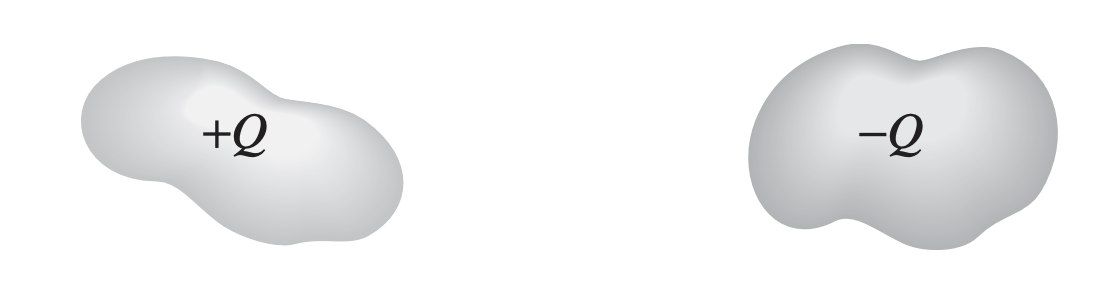
\includegraphics[width=0.65\linewidth]{figure/image35.png}
    \caption{Conduttori carichi con carica $+q$ e $-q$}
    \label{fig:chapter_7_6}
\end{figure}

Dato che il potenziale sui condensatori è costante, possiamo parlare senza ambiguità della differenza di potenziale tra i due conduttori 

\begin{equation*}
    V = V_{+} - V_{-} = \int_{-}^+ \mathbf{E} \cdot d \mathbf{s}
\end{equation*}

Non sappiamo la distribuzione delle cariche sui condensatori, tuttavia sappiamo che $\mathbf{E}$ è proporzionale a $q$. Dalla \ref{eq:campo_elettrostatico_continuo} sappiamo 

\begin{equation*}
    \mathbf{E} = \frac{1}{4 \pi \varepsilon_0} \int_{\tau} \frac{\rho}{r^2} \mathbf{u}_r \ d\tau
\end{equation*}

Quindi se raddoppiamo la carica totale sui condensatori, raddoppiamo $\rho$ e raddoppiamo anche il modulo di $\mathbf{E}$. \\

Dato che $\mathbf{E}$ è proporzionale a $q$, lo sarà anche $V$, allora andiamo a chiamare questa costante di proporzionalità \emph{capacità}. 

\begin{tcolorbox}[colback=yellow!10!white, colframe=orange!70!black, boxrule=0.8pt]
\begin{equation}
    C = \frac{q}{V}
\end{equation}
\end{tcolorbox}

Dove, in questo caso, $V$ rappresenta la \emph{differenza di potenziale tra i conduttori}. \\

Un sistema in cui tra i due \mkeyword{induzione completa} conduttori c'è induzione completa, cioè un sistema in cui tutte le linee di forza partono da un conduttore \mkeyword{condensatore} e finiscono nell'altro, prende il nome di \emph{condensatore}, mentre i due conduttori prendono il nome di armature del condensatore. \\

\newpage

Analizziamo alcuni semplici casi

\subsection{Condensatore piano} 

Un condensatore piano è formato da due piatti piani e paralleli di area $\Sigma$ posti a distanza $h$ su cui sono presenti cariche opposte $+q$ e $-q$

\begin{figure} [h]
    \centering
    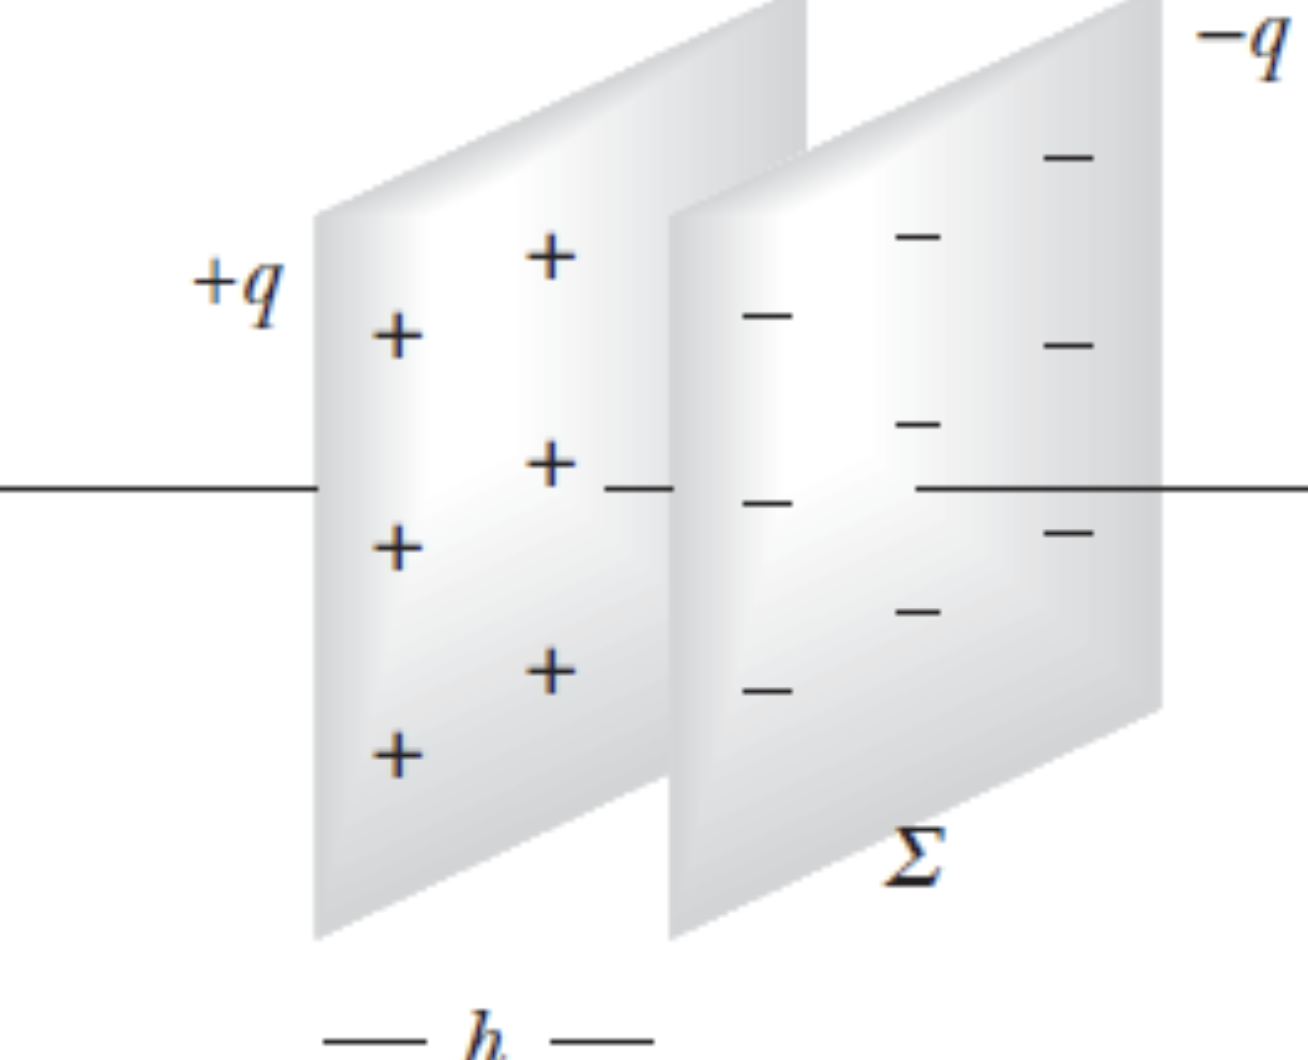
\includegraphics[width=0.4\linewidth]{figure/image36.png}
    \caption{Condensatore piano}
    \label{fig:chapter_7_7}
\end{figure}

La carica positiva $q$ è distribuita con densità uniforme $\sigma$ sull'armatura positiva e quella negativa $-q$ con densità uniforme $-\sigma$ sull'armatura negativa. Il campo interno è costante e quindi si ha

\begin{equation}
    \mathbf{E} = \frac{\sigma}{\varepsilon_0} \mathbf{u}_n \quad , \quad V_1 - V_2 = E \ h = \frac{\sigma}{\varepsilon_0} h = \frac{\sigma \Sigma}{\varepsilon_0 \Sigma} h = \frac{q}{\varepsilon_0 \Sigma} h 
\end{equation}

Si deduce quindi che la capacità di un condensatore piano è data da 

\begin{tcolorbox}[colback=yellow!10!white, colframe=orange!70!black, boxrule=0.8pt]
\begin{equation}
    C = \frac{\varepsilon_0 \Sigma}{h}
\end{equation}
\end{tcolorbox}

\subsection{Condensatore sferico}

Un condensatore sferico è un condensatore formato da due conduttori concentrici di forma sferica. In ciascun punto dell'intercapedine il campo elettrico ha simmetria radiale e un orientamento che dipende dai segni delle cariche delle due armature. \\

\begin{figure} [h]
    \centering
    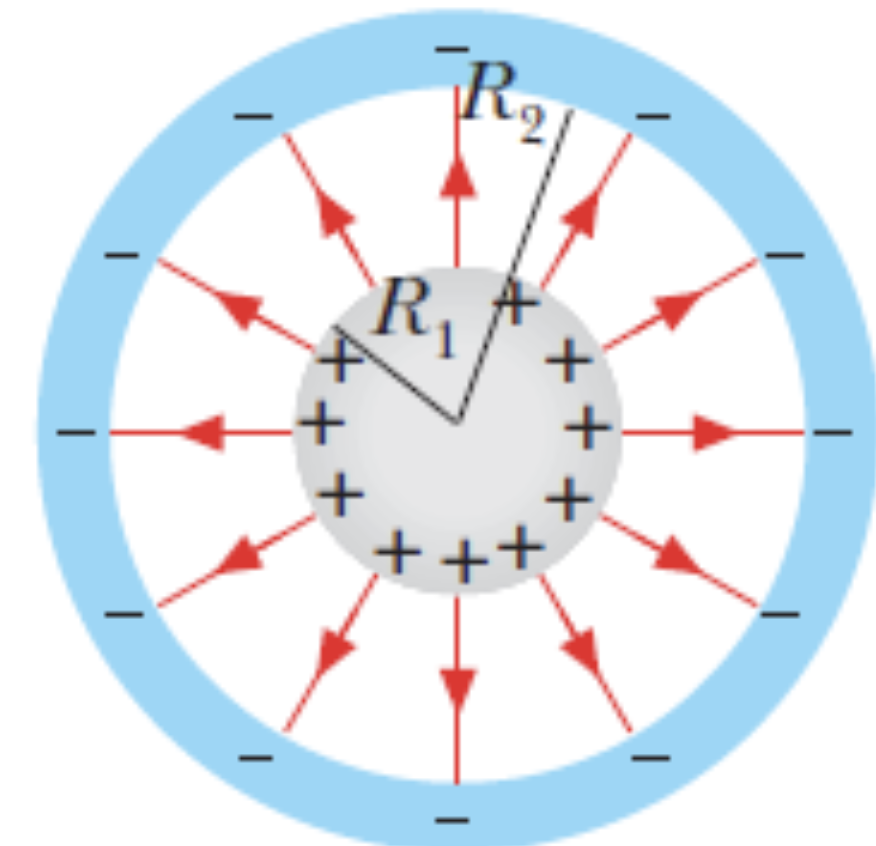
\includegraphics[width=0.4\linewidth]{figure/image37.png}
    \caption{Condensatore sferico}
    \label{fig:chapter_7_8}
\end{figure}

\' E possibile dimostrare che la capacità di questo condensatore è 

\begin{tcolorbox}[colback=yellow!10!white, colframe=orange!70!black, boxrule=0.8pt]
\begin{equation}
    C = 4 \pi \varepsilon_0 \frac{R_1 R_2}{R_2 - R_1}
\end{equation}
\end{tcolorbox}

Dove $R_1$ è il raggio della sfera interna, mentre $R_2$ quello della sfera esterna. 

\subsection{Condensatore cilindrico}

Un condensatore cilindrico è un condensatore costituito da due conduttori cilindrici coassiali. Il campo all'interno di questo condensatore è perpendicolare all'asse e radiale rispetto alla distribuzione di carica. \\

\begin{figure} [h]
    \centering
    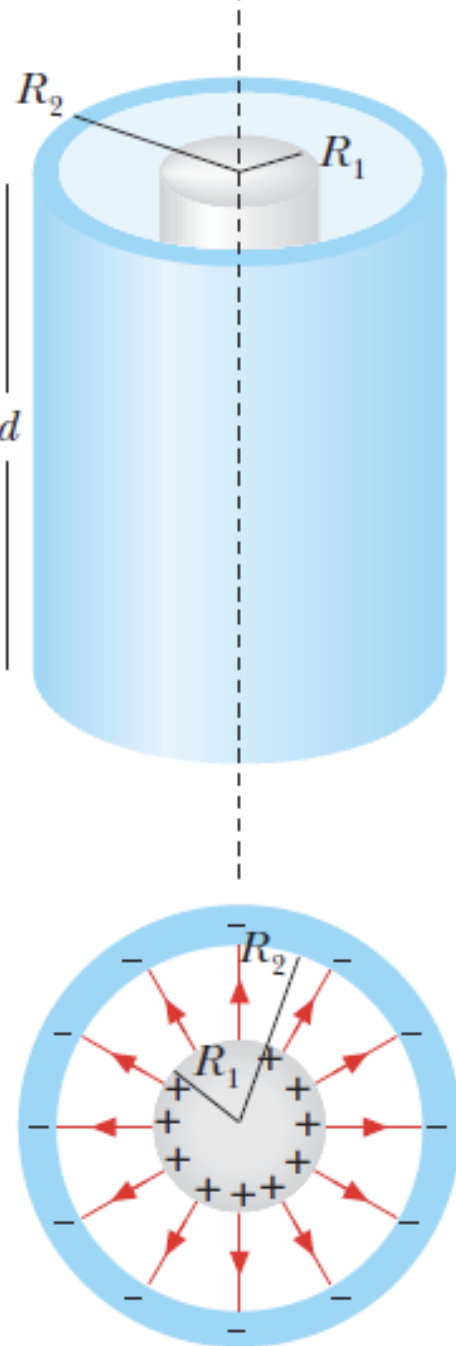
\includegraphics[width=0.25\linewidth]{figure/image38.png}
    \caption{Conduttore cilindrico}
    \label{fig:chapter_7_9}
\end{figure}

\' E facile dimostrare che la capacità di questo condensatore è 

\begin{tcolorbox}[colback=yellow!10!white, colframe=orange!70!black, boxrule=0.8pt]
\begin{equation}
    C = \frac{2 \pi \varepsilon_0 d}{\ln \left(\frac{R_2}{R_1} \right)}
\end{equation}
\end{tcolorbox}

\newpage

\section{Energia elettrostatica per i condensatori}

Il processo di carica di un condensatore, in cui si passa dalla situazione di carica zero sulle armature alla situazione $+q$, $-q$ con una differenza di potenziale $V = q/C$ tra le armature, consiste in definitiva in una separazione di cariche e richiede un determinato lavoro che, essendo il campo conservativo, dipende soltanto dallo stato iniziale e dallo stato finale, ma non dalle modalità con cui avviene il processo. \\

Per eseguire il calcolo possiamo immaginare quindi che la carica di un condensatore avvenga per processi elementari, spostando una carica $dq'$ da un'armatura all'altra, così che alla fine una carica $+q$ è stata trasferita alla seconda armatura, lasciando la prima con una carica $ - q$, e si è stabilita tra le armature la differenza di potenziale elettrostatico V; la carica totale è in ogni istante nulla.\\

Se in una fase intermedia del processo la differenza di potenziale elettrostatico tra le armature è $V'$, in quanto è già stata trasferita la carica $q' = CV'$, il lavoro fatto da un agente esterno per spostare l'ulteriore carica $dq'$ attraverso la differenza di potenziale elettrostatico $V'$ è

\begin{equation}
    dW =  V' dq' = \frac{q'}{C} dq'
\end{equation}

E quindi il lavoro complessivo per effettuare la separazione delle cariche è 

\begin{equation}
    W = \int dW = \int_0 ^q \frac{q'}{C} \ dq' = \frac{q^2}{2C}
\end{equation}

Questo lavoro, effettuato contro la forza elettrostatica che si oppone a un accumulo di cariche dello stesso segno, viene immagazzinato sotto forma di energia elettrostatica, quindi si ha 

\begin{tcolorbox}[colback=yellow!10!white, colframe=orange!70!black, boxrule=0.8pt]
\begin{equation}
    U_e = \frac{1}{2} \frac{q^2}{C} = \frac{1}{2} CV^2 = \frac{1}{2} q V
\end{equation}
\end{tcolorbox}

\section{Forza tra le armature di un condensatore}

Abbiamo trovato che l'energia elettrostatica di un condensatore dipende solo dalla geometria di quest'ultimo e dalla carica sulle armature, allora se vogliamo trovare la forza che agisce sulle armature possiamo sfruttare il fatto che 

\begin{tcolorbox}[colback=yellow!10!white, colframe=orange!70!black, boxrule=0.8pt]
\begin{equation}
    \mathbf{F} = - \nabla U_e = - \frac{q^2}{2} \nabla \left( \frac{1}{C} \right)
\end{equation}
\end{tcolorbox}

Questo vale quando \emph{la carica sulle armature è mantenuta costante}

\newpage

\subsection{Forza tra le armature di un condensatore a potenziale costante}

Invece che a carica costante il processo di spostamento dell'armatura può avvenire a differenza di potenziale elettrostatico costante: si connettono le armature ai poli di un generatore di forza elettromotrice, che è un dispositivo in grado di mantenere costante la differenza di potenziale tra esse. Di conseguenza, quando l'armatura positiva si sposta avvicinandosi all'altra armatura, V resta costante, C aumenta e quindi q deve aumentare: il processo comporta ora uno spostamento di carica da un'armatura all'altra, con spesa di lavoro. 
Pertanto quando andremo a trovare l'energia totale del sistema \emph{dovremo considerare sia l'energia dovuta alla distribuzione di carica, sia quella dovuta al generatore}.\\

La variazione di energia elettrostatica è 

\begin{equation}
    dU_e = d \left(\frac{1}{2} CV^2\right) = \frac{V^2}{2} \ dC
\end{equation}

Che è positivo. Mentre il lavoro per lo spostamento della carica $dq = V dC$ è 

\begin{equation}
    dW_{\text{gen}} = V \ dq = V^2 \ dC = - dU_{\text{gen}} 
\end{equation}

Che è negativo, in quanto è fornito a spese dell'energia interna.\\

Allora l'energia totale del sistema varia come 

\begin{equation}
    dU = dU_e + dU_{\text{gen}} = - dU_e
\end{equation}

Pertanto si ha in questo caso 

\begin{tcolorbox}[colback=yellow!10!white, colframe=orange!70!black, boxrule=0.8pt]
\begin{equation}
    \mathbf{F} = - \nabla U  = \nabla U_e = \frac{1}{2} V^2 \ \nabla C
\end{equation}
\end{tcolorbox}


\chapter{Unicità delle soluzioni con condizioni al contorno}

Abbiamo visto che il comportamento di un campo elettrostatico può essere descritto dalle equazioni differenziali 

\begin{align*}
    \nabla \cdot \mathbf{E} = \frac{\rho}{\varepsilon_0} \quad, \quad \nabla \times \mathbf{E} = 0 \quad , \quad \mathbf{E} = - \nabla V
\end{align*}

che combinate danno le \emph{equazione di Poisson} ed \emph{equazione di Laplace}

\begin{equation*}
    \nabla ^2 V = - \frac{\rho}{\varepsilon_0} \quad , \quad \nabla^2 V = 0
\end{equation*}

Se nei problemi elettrostatici comparissero sempre distribuzioni localizzate di carica, discrete o continue, senza superfici di confine, la soluzione generale \ref{eq:potenziale_senza_condizione} sarebbe quella più diretta e più conveniente per ogni problema. Non ci sarebbe alcun bisogno delle equazioni di Poisson o di Laplace. Nella realtà, molti, se non la maggior parte, dei problemi dell'elettrostatica sono formulati in regioni finite di spazio contenenti o meno delle cariche, e con delle condizioni al contorno assegnate sulle superfici di confine. Quindi la \ref{eq:potenziale_senza_condizione} non è più così utile se non in casi semplici. 

\section{Condizioni al contorno di Dirichlet o di Neumann}

Quali condizioni al contorno sono appropriate per l'equazione di Poisson (o di Laplace) per garantire l'esistenza di un'unica soluzione regolare entro una regione limitata?\\

L'esperienza fisica ci porta a \mkeyword{problema di Dirichlet} ritenere che la specificazione del potenziale su una superficie chiusa (come nel caso di un sistema di conduttori) definisca un univoco problema di potenziale. Questo è chiamato \emph{problema di Dirichlet} o \emph{condizione al contorno di Dirichlet}. \\

\' E similmente \mkeyword{condizione al contorno di Neumann} plausibile che la specificazione del campo elettrico (derivata normale del potenziale) ovunque sulla superficie (corrispondendo ad una data densità superficiale di carica) definisca pure un problema univoco. Questo è chiamata \emph{condizione al contorno di Neumann}. \\

Andiamo adesso a mostrare l'unicità della soluzione all'equazione di Poisson all'interno di un volume $\tau$ con condizioni al bordo di Dirichlet o Neumann sulla superficie chiusa $\Sigma$ che lo delimita. \\

Supponiamo per assurdo che esistano due funzioni potenziali $V_1$ e $V_2$ che soddisfano le condizioni al contorno. Allora possiamo andare a definire una funzione $f$ come

\begin{equation*}
    f = V_1 - V_2
\end{equation*}

Allora deve valere

\begin{equation*}
    \nabla ^2 f = \nabla^2V_1 - \nabla^2 V_2 = 0 \quad , \quad f(\Sigma) = V_1(\Sigma) - V_2(\Sigma) = 0 
\end{equation*}

Consideriamo 

\begin{equation*}
    \nabla (f \nabla f) = (\nabla f)^2 + f \nabla^2f
\end{equation*}

Usando il teorema della divergenza 

\begin{equation*}
    \int_{\tau} \nabla(f \nabla f) d\tau= \int_{\Sigma} f (\nabla f) d \Sigma \ \hat{n} = 0
\end{equation*}

L'ultima uguaglianza è dovuta al fatto che $f$ è nulla su tutta la superficie. Allora vale

\begin{equation*}
    \int_{\tau} \nabla(f \nabla f) d\tau = \int_{\tau} (\nabla f)^2 d \tau + \int_{\tau} f(\nabla^2 f) d\tau = 0
\end{equation*}

In particolare $\nabla^2 f = 0$, quindi risulta 

\begin{equation*}
    \int_{\tau} (\nabla f)^2 d \tau= 0
\end{equation*}

Ma poiché $(\nabla f)^2 \ge 0$, deve essere $\nabla f = 0$, quindi $f(\mathbf{r})$ è costante e dato che $f(\Sigma) = 0$ risulta che 

\begin{equation}
    V_1 = V_2
\end{equation}

In opposizione con la tesi. Abbiamo così dimostrato l'unicità del potenziale con condizioni al bordo fissate. 

\newpage

\section{Soluzione formale del problema elettrostatico dei valori al contorno con la funzione di Green}

Per affrontare le condizioni al contorno è necessario sviluppare qualche nuovo strumento matematico, ossia la delta di Dirac e le identità di Green.


\subsection{Delta di Dirac e Identità di Green}

La delta di Dirac \mkeyword{Delta di Dirac} è una funzione matematica impropria, indicata, in una dimensione, con $\delta (x -a)$ con le proprietà: \\

\begin{enumerate}
    \item $\delta (x - a) = 0$ per $x \neq a$ \\
    \item $\int \delta(x -a) dx = 1$ se la regione di integrazione include $x = a$, altrimenti vale zero. \\
    \item $\int f(x) \delta (x -a) dx = f(a)$ \\
    \item $\int f(x) \delta ' (x - a) dx = - f' (a)$, dove l'apice indica la derivazione rispetto all'argomento. \\
\end{enumerate}

Si può dare alla delta un significato intuitivo, ma non rigoroso, con il limite di una curva piccata, come gaussiana, che diventa sempre più stretta ma sempre più alta, in modo che l'area sottesa resti costante. \\

Introduciamo adesso le due identità di Green. Queste si ottengono da semplici applicazioni del teorema della divergenza. \footnote{Per vedere la derivazione delle due identità consultare \cite{ElettrodinamicaClassica} o un buon manuale di Analisi 2} \\

Siano \mkeyword{Prima identità di Green} $\phi$ e $\psi$ due campi scalari arbitrari, sia $\tau$ un volume delimitato da una superficie $\Sigma$ e sia $\partial / \partial n$ la derivata normale alla superficie $\Sigma$, la \emph{prima identità di Green} afferma

\begin{tcolorbox}[colback=yellow!10!white, colframe=orange!70!black, boxrule=0.8pt]
\begin{equation}
    \int _{\tau} (\phi \nabla^2 \psi + \nabla \phi \cdot \nabla \psi) \ d\tau = \oint _{\Sigma} \phi \frac{\partial \psi}{\partial n} \ d\Sigma 
    \label{eq:prima_identità_Green}
\end{equation}
\end{tcolorbox}

Se riscriviamo \mkeyword{Seconda identità di Green} la \ref{eq:prima_identità_Green} scambiando $\psi$ e $\phi$ e ne sottraiamo il risultato, otteniamo la seconda \emph{seconda identità di Green}

\begin{tcolorbox}[colback=yellow!10!white, colframe=orange!70!black, boxrule=0.8pt]
\begin{equation}
    \int_{\tau} (\phi \nabla^2 \psi - \psi \nabla^2 \phi) \ d \tau =\oint_{\Sigma} \left [ \phi \frac{\partial \psi}{\partial n} - \psi \frac{\partial \phi}{\partial n} \right ] \ d \Sigma
    \label{eq:seconda_identità_Green}
\end{equation}
\end{tcolorbox}

\newpage

Adesso possiamo andare a ricavare una soluzione formale del problema con valori al contorno.\\

Se andiamo a porre 

\begin{equation}
    \psi \equiv \frac{1}{R} = \frac{1}{|\mathbf{r} - \mathbf{r'}|}
\end{equation}

Dove $r$ è il punto di osservazione e $r'$ è la variabile di integrazione. \' E possibile ottenere che 

\begin{equation*}
    \nabla^2 \left( \frac{1}{R} \right ) = -4 \pi \delta (\mathbf{r} - \mathbf{r'})
\end{equation*}

Inoltre poniamo $\phi = V$, il potenziale scalare, ed utilizziamo $\nabla^2 V = - \rho/\varepsilon_0$. \\
In questo modo, sostituendo nella \ref{eq:seconda_identità_Green} si ottiene 

\begin{equation*}
    \int_{\tau} \left [ -4 \pi V(\mathbf{r '}) \delta(\mathbf{r} - \mathbf{r'}) + \frac{1}{\varepsilon_0 R} \rho (\mathbf{r '})  \right ] d\tau = \oint_{\Sigma} \left[ V \frac{\partial}{\partial n'} \left(  \frac{1}{R}\right ) - \frac{1}{R} \frac{\partial V}{\partial n'}  \right ] \ d \Sigma'
\end{equation*}

Se il punto $\mathbf{r}$ si trova interno al volume $\tau$, si ha

\begin{equation*}
    \int_{\tau} [-4 \pi V(\mathbf{r'}) \delta(\mathbf{r} - \mathbf{r'})] d \tau = -4 \pi V(\mathbf{r})
\end{equation*}

Quindi sostituendo e isolando il potenziale si ottiene 

\begin{equation}
    V(\mathbf{r}) = \frac{1}{4 \pi \varepsilon_{0}} \int_{\tau} \frac{\rho(\mathbf{r'})}{R} d \tau + \frac{1}{4 \pi} \oint \left [ \frac{1}{R} \frac{\partial V}{\partial n'} - V \frac{\partial}{\partial n'} \left ( \frac{1}{R} \right ) \right ] \ d \Sigma' 
    \label{eq:falsa_soluzione_potenziale}
\end{equation}

Un primo fatto da notare è che se la superficie $\Sigma$ va all'infinito e il campo elettrico su $\Sigma$ decresce più rapidamente di $R^{-1}$, allora l'integrale di superficie si annulla e la \ref{eq:falsa_soluzione_potenziale}
riproduce esattamente la \ref{eq:potenziale_senza_condizione}. \\

Tuttavia quella ottenuta \emph{non è la soluzione di un problema di valori al contorno}, perché una specificazione arbitraria sia di $V$ sia di $\partial V / \partial n$ è una sovradeterminazione del problema. \\

Tuttavia possiamo andare a modificare la forma della \ref{eq:falsa_soluzione_potenziale} in modo che soddisfi solo una condizione. \\
Infatti, un passo fondamentale nella derivazione della \ref{eq:falsa_soluzione_potenziale} è stata la relazione

\begin{equation}
    \nabla^2 \left (\frac{1}{|\mathbf{r} - \mathbf{r'}|} \right ) = - 4 \pi \delta (\mathbf{r} - \mathbf{r'})
    \label{eq:relazione}
\end{equation}

Ma la funzione $1 / |\mathbf{r} - \mathbf{r'}|$ è solo una di una classe di funzioni dipendenti dalle variabili $\mathbf{r}$ e $\mathbf{r'}$, chiamate \emph{funzioni di Green} \mkeyword{funzioni di Green}, che soddisfano la \ref{eq:relazione}. In generale 

\begin{equation}
    \nabla ^2 G(\mathbf{r}, \mathbf{r'}) = -4 \pi \delta (\mathbf{r} -\mathbf{r'})
\end{equation}

dove

\begin{equation}
    G(\mathbf{r}, \mathbf{r'}) = \frac{1}{|\mathbf{r} - \mathbf{r'}|} + F(\mathbf{r}, \mathbf{r'})
    \label{eq:funzione_Green}
\end{equation}

e la funzione $F$ è una funzione armonica, che quindi soddisfa il teorema di Laplace entro il volume $\tau$:

\begin{equation*}
    \nabla ^2 F(\mathbf{r}, \mathbf{r'}) = 0
\end{equation*}

Quindi, ponendo adesso $\phi = V$ e $\psi = G(\mathbf{r}, \mathbf{r'})$ e ripetendo tutti i passaggi si ottiene 

\begin{tcolorbox}[colback=yellow!10!white, colframe=orange!70!black, boxrule=0.8pt]
\begin{equation}
    V(\mathbf{r}) = \frac{1}{4 \pi \varepsilon_{0}} \int_{\tau} \rho(\mathbf{r'}) G(\mathbf{r}, \mathbf{r'}) d \tau + \frac{1}{4 \pi} \oint \left [ G(\mathbf{r}, \mathbf{r'}) \frac{\partial V}{\partial n'} - V(\mathbf{r'}) \frac{\partial G(\mathbf{r}, \mathbf{r'})}{\partial n'} \right ] \ d \Sigma' 
    \label{eq:soluzione_generale_potenziale_contorno}
\end{equation}
\end{tcolorbox}

La libertà disponibile nella definizione di $G$ significa che possiamo fare in modo che l'integrale di superficie dipenda solo dal tipo scelto di condizione di contorno. \\

Per \emph{condizioni al contorno di Dirichlet} richiediamo \footnote{Per le condizioni al contorno di Neumann si consiglia di guardare \cite{ElettrodinamicaClassica}}

\begin{equation}
    G_D(\mathbf{r}, \mathbf{r'}) = 0 \quad \text{per $\mathbf{r'}$ su $\Sigma$}
    \label{eq:condizione_di_Dirichlet}
\end{equation}

Allora il primo termine dell'integrale di superficie nella \ref{eq:soluzione_generale_potenziale_contorno} si annulla e la soluzione è 

\begin{tcolorbox}[colback=yellow!10!white, colframe=orange!70!black, boxrule=0.8pt]
\begin{equation}
    V(\mathbf{r}) = \frac{1}{4 \pi \varepsilon_{0}} \int_{\tau} \rho(\mathbf{r'}) G_D(\mathbf{r}, \mathbf{r'}) d \tau - \frac{1}{4 \pi} \oint V(\mathbf{r'}) \frac{\partial G_D(\mathbf{r}, \mathbf{r'})}{\partial n'} \ d \Sigma'
\end{equation}
\end{tcolorbox}

Osserviamo che le funzioni di Green soddisfano le semplici condizioni al contorno \ref{eq:condizione_di_Dirichlet}, che non dipendono dalla forma dettagliata dei valori al contorno di Dirichlet (o di Neumann). Nonostante ciò \emph{spesso è piuttosto complicato, se non impossibile, determinare $G(\mathbf{r}, \mathbf{r'})$} a causa della sua dipendenza dalla forma della superficie $\Sigma$. 

\newpage

%\subsection{Metodo delle cariche immagini}

%Consideriamo un conduttore $C$ con potenziale $V_0$ (essendo un conduttore la sua superficie è equipotenziale) e in prenseza di esso, una o più cariche puntiformi localizzate $Q_i$. \\

%Se la geometria del coduttore è semplice(ad esempio piana, o sferica, ecc.) allora il problema dell'elettrostatica può essere risolto in maniera semplice ed efficace mediante il metodo cosiddetto delle \emph{cariche immagine}. \\ Questo metodo consiste nell'immaginare che il conduttore sia sostituito con una o più cariche puntiformi $Q'_i$ situate, rispetto al conduttore, dalla parte opposta rispetto alle $Q_i$, e disposte in modo che la somma dei potenziali generati dalle $Q_i$ e dalle $Q'_i$ sia $V_0$ su $\Sigma$.\\ 

%L'insieme delle cariche $Q_i$ e $Q'_i$ genera allora, in assenza del conduttore, nella porzione $\tau$ di spazio vuoto prospiciente a $\Sigma$ dalla parte delle $Q_i$, la stessa configurazione di potenziale generata dalle $Q_i$ e dalla distribuzione (incognita) delle cariche presenti per induzione su $\Sigma$.\\

%Ciò è conseguenza del \textit{teorema di unicità}, considerato che sia il sistema $(Q_i + S)$ che il sistema $(Q_i + Q'_i)$ hanno, nella porzione di spazio $\tau$, la stessa distribuzione di carica (rappresentata dalle $Q_i$) e le stesse condizioni al contorno (rappresentate da $V_0$ su $\Sigma$, e da $V \to 0$ all'infinito).\\

%Il vantaggio del metodo delle cariche immagine consiste nel fatto che il potenziale generato dal sistema $(Q_i + Q'_i)$ è facilmente calcolabile mediante la \ref{eq:potenziale_per_più_cariche}.


\chapter{Problemi con condizioni al contorno}

Molti problemi in elettrostatica riguardano condizioni al contorno dove è specificato il potenziale o la densità di carica superficiale. \\ La soluzione formale a questi problemi è stata introdotta nel capitolo precedente, utilizzando il metodo della funzione di Green; tuttavia, come accennato, nelle situazioni pratiche trovare la corretta funzione di Green non è facile. \\

Per questo sono stati sviluppati dei metodi per risolvere i problemi di elettrostatica riguardanti le condizioni al bordo. Di seguito si riportano le seguenti tecniche:

\begin{enumerate}
    \item \emph{metodo delle cariche immagine}, lontano dal metodo usuale di trovare la funzione di Green
    \item \emph{metodo di separazione delle variabili}
    \item \emph{analisi agli elementi finiti} \footnote{Non tratteremo questo metodo}
\end{enumerate}

\section{Metodo delle cariche immagine}

Il metodo delle cariche immagine riguarda il problema di una o più cariche in presenza di una condizione di contorno, per esempio un conduttore messo a terra o isolato con potenziale fissato. \\

Con condizioni geometricamente favorevoli è possibile riportare il sistema iniziale a un sistema formato da un numero finito di cariche posizionate in precisi punti dello spazio, al di fuori della regione di nostro interesse, in modo che il loro potenziale rispetti le condizioni al bordo del problema. \\

L'insieme delle cariche genera allora, in assenza del conduttore, nella porzione di spazio vuoto prospiciente al contorno, la stessa configurazione di potenziale del sistema iniziale. \\ 
Ciò è conseguenza del \textit{teorema di unicità}.\\

Di seguito si riportano alcuni casi importanti. 

\subsection{Carica posizionata davanti a un piano conduttore infinito messo a terra}

Una carica puntiforme positiva $q$ è posta di fronte a una lastra conduttrice a potenziale zero, da cui dista $x$. \\
Per induzione completa, la carica $+q$ induce una carica $-q$ sulla lastra, distribuita con densità superficiale $\sigma$ in modo che la carica $q$ e la carica indotta diano in ogni punto della superficie un valore uniforme e, in particolare, nullo del potenziale elettrostatico. \\
Il potenziale elettrostatico dovuto alla carica $q$ in un punto del piano distante $r$ da $q$ è 

\begin{equation*}
    V_q = \frac{q}{4 \pi \varepsilon_0 r}
\end{equation*}

e la carica indotta deve generare in quel punto il potenziale

\begin{equation*}
    V_i = - \frac{q}{4 \pi \varepsilon_0 r}
\end{equation*}

Una situazione di questo genere si può realizzare, in ogni punto del piano, ponendo una carica immagine $-q$ in posizione simmetrica a quella della carica $q$ rispetto al piano. 

\begin{figure} [h]
    \centering
    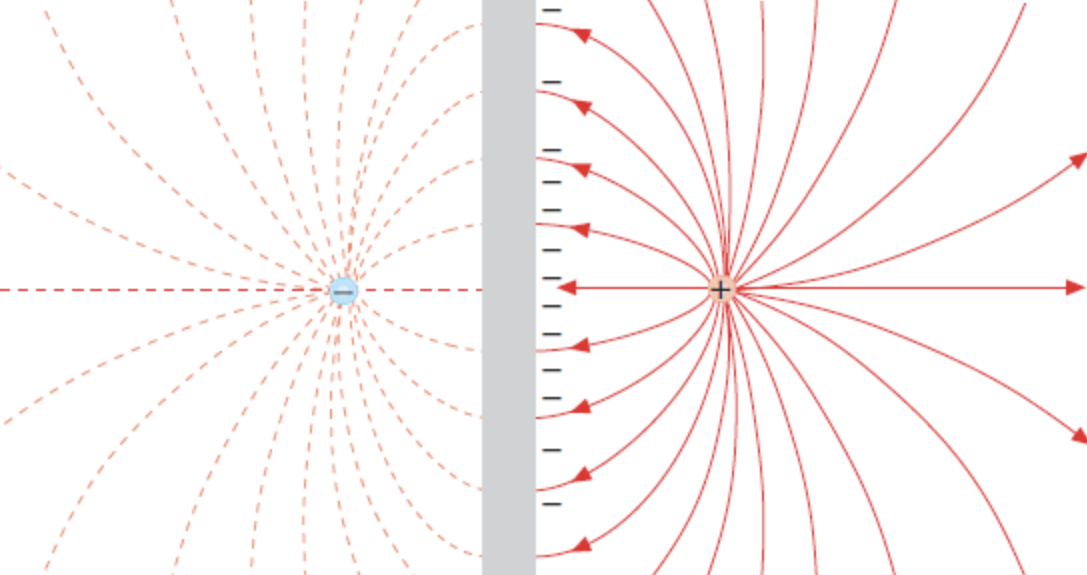
\includegraphics[width=0.4\linewidth]{figure/image19.png}
    \caption{Carica $q$ davanti a piano infinito}
    \label{fig:chapter_9_1}
\end{figure}

\subsection{Carica in presenza di una sfera conduttrice carica messa a terra}

Consideriamo una carica $q$ in posizione $\mathbf{r}$ rispetto all'origine $O$ del sistema, il quale è il centro di una sfera conduttrice messa a terra di raggio $a$. \\

Cerchiamo il potenziale $V(\mathbf{x})$ tale per cui $V(|\mathbf{x}| = a) = 0$. \\

\begin{figure} [h]
    \centering
    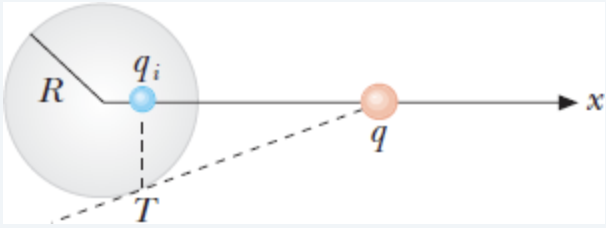
\includegraphics[width=0.4\linewidth]{figure/image20.png}
    \label{fig:chapter_9_2}
\end{figure}

Per simmetrica è evidente che l'immagine $q'$ sarà posizionata lungo il raggio che congiunge l'origine e la carica $q$. \\ Se la $q$ è \emph{esterna} alla sfera, la posizione $\mathbf{r'}$ della carica immagine sarà interna alla sfera ($\mathbf{|r'| < a}$). Il potenziale dovuto a $q$ e $q'$ risulta essere


\begin{equation*}
    V(\mathbf{x}) = \frac{q/4\pi \varepsilon_0}{|\mathbf{x} - \mathbf{r}|} + \frac{q'/4 \pi \varepsilon_0}{|\mathbf{x} - \mathbf{r'}|}
\end{equation*}

Dobbiamo scegliere $q'$ e $|\mathbf{r'}|$ in modo che il potenziale si annulli per $|\mathbf{x}| = a$. Scegliendo degli opportuni angoli e sfruttando alcune proprietà di similitudine tra triangoli si arriva facilmente al risultato. 

\begin{tcolorbox}[colback=yellow!10!white, colframe=orange!70!black, boxrule=0.8pt]
\begin{equation}
    q' = - \frac{a}{r}q \quad , \quad r' = \frac{a^2}{r}
\end{equation}
\end{tcolorbox}

La densità di carica indotta sulla superficie della sfera può essere calcolata dal tramite il gradiente del potenziale sulle superficie.

\begin{equation}
    \sigma = - \varepsilon_0 \nabla V(|\mathbf{x} = a|) = - \frac{q}{4 \pi a^2} \left ( \frac{a}{r} \right ) \frac{1 - \frac{a^2}{r^2}}{\left ( 1 + \frac{a^2}{r^2} - 2 \frac{a}{r} \cos \gamma \right )}
\end{equation} 

Dove $\gamma$ è l'angolo tra $\mathbf{x}$ e $\mathbf{r}$.\\

La carica totale indotta sul conduttore si trova facilmente utilizzando il teorema del Gauss. Immaginiamo una superficie gaussiana che avvolge in modo molto "aderente" il conduttore considerato, allora sappiamo che vale

\begin{equation*}
    \oint_{\Sigma} \mathbf{E} \cdot \mathbf{u}_n \ d\Sigma = \frac{Q_{\text{indotta}}}{\varepsilon_0}   
\end{equation*}

Ma dato che le cariche immagine devono essere interne al condensatore, si deve avere 

\begin{equation*}
    \oint_{\Sigma} \mathbf{E} \cdot \mathbf{u}_n \ d\Sigma = \frac{\sum q_{\text{immagine}}}{\varepsilon_0}   
\end{equation*}

Quindi 

\begin{tcolorbox}[colback=yellow!10!white, colframe=orange!70!black, boxrule=0.8pt]
\begin{equation}
    Q_{\text{indotta}} = \sum q_{\text{immagine}} 
\end{equation}
\end{tcolorbox}

Questo è un risultato del tutto generale. \\

La forza agisce sulla carica $q$ può essere calcolata in vari modi, il più semplice tra questi è trovare la forza tra la carica $q$ e la carica immagine $q'$.

\subsection{Carica in presenza di una sfera conduttrice carica isolata}

Consideriamo una sfera conduttrice carica con una carica $Q$ e una carica puntiforme q.\\

Da un punto di vista operativo possiamo pensare di avere inizialmente una sfera conduttrice messa a terra e una carica puntiforme $q$, in modo da utilizzare il metodo descritto sopra e trovare una carica immagine $q'$. \\

Possiamo poi scollegare da terra la sfera e aggiungere a questa una carica $(Q-q')$. Questo porta la sfera ad avere una carica totale $Q$. Per trovare il potenziale si nota che la carica aggiunta $(Q-q')$ si disporrà \emph{uniformemente} sulla superficie della sfera, poiché la forza elettrostatica dovuta a $q$ è bilanciata dalla carica $q'$. \\

\newpage

Allora il potenziale dovuto all'aggiunta della carica $(Q - q)$ sarà lo stesso di una carica puntiforme con la stessa carica situato nell'origine (questo per punti esterni alla sfera).

\begin{equation}
    V(\mathbf{x}) = \frac{1}{4 \pi \varepsilon_0} \left [ \frac{q}{|\mathbf{x} - \mathbf{r}|} - \frac{aq}{r|\mathbf{x} - \frac{a^2}{r^2} \mathbf{r}|} + \frac{Q + \frac{a}{r}q}{|\mathbf{x}|} \right ]
    \label{eq:7.4}
\end{equation}

Come nei casi precedenti per trovare la forza che agisce sulla carica $q$, basta trovare la forza tra $q$ e le due cariche immagine $q'$ e $(Q-q')$ .

\subsection{Carica in presenza di una sfera conduttrice a potenziale fissato}

Un altro problema che possiamo discutere semplicemente è quello una carica $q$ vicina a una sfera conduttrice a potenziale fissato $V$.\\

Possiamo agire esattamente come per il caso precedente, l'unica cosa è che al posto della carica $(Q-q')$ aggiungiamo la carica $4 \pi \varepsilon_0 Va$. Questo si vede dalla \ref{eq:7.4}, in quanto per $|\mathbf{x}| = a$ i primi due termini si cancellano (per costruzione) e l'ultimo termine deve essere uguale a $V$ come richiesto. 

\begin{equation}
    V(\mathbf{x}) = \frac{1}{4 \pi \varepsilon_0} \left [ \frac{q}{|\mathbf{x} - \mathbf{r}|} - \frac{aq}{r|\mathbf{x} - \frac{a^2}{r^2} \mathbf{r}|} \right ] + \frac{Va}{|\mathbf{x}|}
\end{equation}

\subsection{Sfera conduttrice in un campo elettrostatico uniforme}

Prima di considerare il caso vero e proprio, è necessario riportare alcune proprietà. \\

\begin{figure} [h]
    \centering
    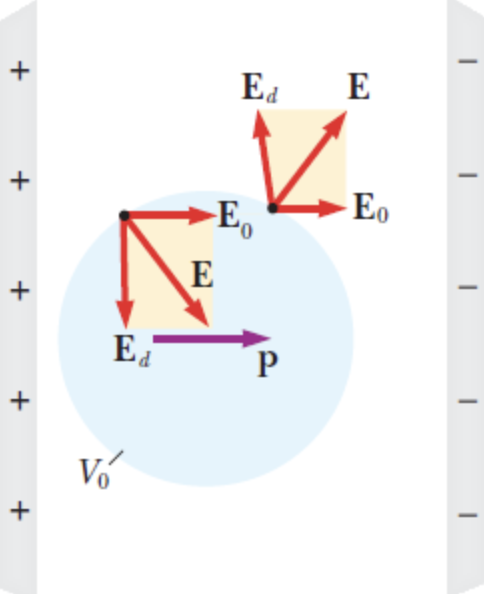
\includegraphics[width=0.25\linewidth]{figure/image21.png}
    \caption{Superficie equipotenziale del dipolo}
    \label{fig:chapter_9_3}
\end{figure}

\'E possibile dimostrare\footnote{Per la dimostrazione guardare \cite{ElettromagnetismoeOnde}, oppure farla a mano} che preso un campo elettrico uniforme $E_0$ e un dipolo parallelo al campo elettrico di momento di dipolo $\mathbf{p}$, esiste una superficie equipotenziale sferica con centro nel dipolo e raggio $R$, dove 

\begin{equation}
    R = \left ( \frac{p}{4 \pi \varepsilon_0 E_0} \right ) ^{1/3}
\end{equation}

Adesso possiamo passare al problema di nostro interesse.

Consideriamo una sfera conduttrice in un campo uniforme, la sua superficie deve essere equipotenziale; ma allora la situazione elettrostatica all'esterno della sfera si può calcolare supponendo di porre nel centro della sfera elettrostatica un \emph{dipolo immagine} con momento di dipolo $\mathbf{p}$ parallelo al campo e il cui momento è determinato dal raggio della sfera e dal valore del campo elettrostatico uniforme:

\begin{tcolorbox}[colback=yellow!10!white, colframe=orange!70!black, boxrule=0.8pt]
\begin{equation}
    p = 4 \pi \varepsilon_0 R^3 E_0
\end{equation}
\end{tcolorbox}

Il campo elettrostatico all'esterno della sfera è dato dalla sovrapposizione di $E_0$ e del campo del dipolo di momento $\mathbf{p}$. 

\begin{figure} [h]
    \centering
    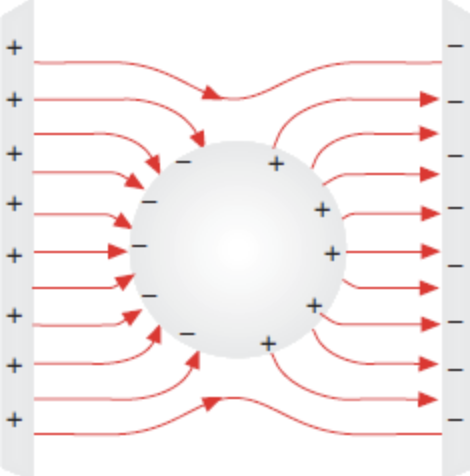
\includegraphics[width=0.35\linewidth]{figure/image22.png}
    \caption{Sfera conduttrice in un campo elettrico uniforme}
    \label{fig:chapter_9_4}
\end{figure}

In particolare il campo elettrico sulla superficie risulta essere 

\begin{equation}
    \mathbf{E} = - \nabla V = - \left ( \frac{\partial V}{\partial r} \right )_{r = R} \mathbf{u}_r = \left ( E_0 \cos \theta + \frac{2p \cos \theta }{4 \pi \varepsilon_0 R^3}\right) \mathbf{u}_r = 3 E_0 \cos \theta  \ \mathbf{u}_r 
\end{equation}

Inoltre possiamo trovare la densità di carica della sfera

\begin{equation}
    \sigma = E \varepsilon_0 = - \varepsilon_0 \frac{\partial V(|\mathbf{x}| = R)}{\partial r} = 3 \varepsilon_0 E_0 \cos \theta
\end{equation}

Si nota che l'integrale di superficie di questa quantità sparisce, quindi non c'è alcuna differenza tra una sfera messa a terra e una isolata. 

\subsection{Carica all'interno di una sfera conduttrice messa a terra}

Consideriamo una carica $q$ all'interno di una sfera conduttrice messa a terra di raggio $a$ a distanza $r$ dal centro della sfera.\\

La situazione è analoga al caso di una carica in presenza di una sfera conduttrice carica discusso sopra, l'unica differenza è che i ruoli della carica reale e della carica immagine sono invertiti, infatti si ha che per ricreare le condizioni al contorno possiamo considerare una carica immagine $q'$ a distanza $r'$ dal centro, dove

\begin{tcolorbox}[colback=yellow!10!white, colframe=orange!70!black, boxrule=0.8pt]
\begin{equation}
    q' = -\frac{r}{a} q \quad , \quad r' = \frac{a^2}{r}
\end{equation}
\end{tcolorbox}

\subsection{Energia del sistema con il metodo delle cariche immagine}

Quando si usa il metodo delle cariche immagine si deve fare attenzione, infatti potremmo farci prendere la mano e assumere che il sistema con il condensatore con condizioni al bordo e il sistema delle cariche immagine siano del \emph{tutto} identici, tuttavia questo \emph{non} è vero. \\

\emph{L'energia non è la stessa}. \\

Consideriamo l'esempio più semplice, quello di una carica $q$ in presenza di un piano conduttore messo a terra. \\
Se consideriamo il sistema ottenuto con il metodo delle cariche immagine, si ottiene che l'energia del sistema è 

\begin{equation*}
    U_{e_1} = - \frac{1}{4 \pi \varepsilon_0} \frac{q^2}{2d}
\end{equation*}

Se adesso, invece, consideriamo il sistema formato dalla carica e dal piano, otteniamo 

\begin{equation*}
    U_{e_2} = \frac{1}{2} \int V \ dq = - \frac{1}{4 \pi \varepsilon_0} \frac{q^2}{4d}
\end{equation*}

Si vede, allora, che $U_{e_1} \neq U_{e_2}$. \\

Riportiamo, allora, un metodo veloce e generale per trovare l'energia di un sistema con condizioni al contorno. \\

Sappiamo che per una distribuzione di cariche (nel caso continuo) vale 

\begin{equation*}
    U_e = \frac{1}{2} \int V \ dq
\end{equation*}

Nel nostro caso possiamo dividere le cariche che si trovano sul condensatore e le cariche reali esterne a quest'ultimo. 

\begin{equation*}
    U_e = \frac{1}{2} \int V_{\text{condensatore}} \ dq + \frac{1}{2} \int V_{\text{esterno}} \ dq
\end{equation*}

Tuttavia stiamo considerando un problema con condizioni al contorno, quindi $V_{\text{condensatore}} = V_0$ e la carica che si trova sul condensatore è esattamente $Q_{\text{condensatore}} = \sum q_{\text{immagine}}$. \\ Mentre il potenziale che si trova sulla p-esima carica reale risulta essere 

\begin{equation*}
    V_p = \sum _i \frac{1}{4\pi \varepsilon_0} \frac{q'_i}{r_{ip}} + \sum_j \frac{1}{4 \pi \varepsilon_0} \frac{q_j}{r_{jp}}
\end{equation*}

Dove $q'_i$ sono le cariche immagine e $q_j$ le cariche reali. 

Allora si ottiene che l'energia $U_e$ del sistema è  

\begin{tcolorbox}[colback=yellow!10!white, colframe=orange!70!black, boxrule=0.8pt]
\begin{equation}
    U_e = \frac{1}{2} V_0 \sum_i q'_i + \frac{1}{2} \sum_p q_p \left( \sum _i \frac{1}{4\pi \varepsilon_0} \frac{q'_i}{r_{ip}} + \sum_{j \neq p} \frac{1}{4 \pi \varepsilon_0} \frac{q_j}{r_{jp}}   \right)
\end{equation}
\end{tcolorbox}

\section{Metodo di separazione delle variabili}

In questa sezione andiamo ad "attaccare" direttamente l'equazione di Laplace, utilizzando il metodo di separazione delle variabili, uno dei metodi preferiti dei fisici per risolvere equazioni differenziali. \\

Il metodo è applicabile quando il potenziale o la densità di carica è specificata al contorno di una certa regione ed è chiesto di trovarne il potenziale all'interno.\\

La strategia di base è molto semplice: \emph{cerchiamo soluzioni esprimibili come prodotto di funzioni dove ciascuna di queste dipende solo da una coordinata}.\\

Tuttavia, i dettagli algebrici per trovare la soluzione particolare da quella generale, ponendo le condizioni al contorno, possono essere formidabili, per questo dedicheremo del tempo per capirne a fondo la matematica.

\subsection{Funzioni ortogonali e sviluppi}

Come accennato sopra, in questa sotto-sezione andremo a riportare alcuni mezzi matematici \emph{necessari} per capire a pieno i passaggi di alcune dimostrazioni e per \emph{risolvere un gran numero di problemi con condizioni al contorno}. \\

Iniziamo introducendo lo spazio $L^p$ \mkeyword{spazio $L^p$} come lo spazio delle funzioni a p-esima potenza sommabile. Si tratta di uno \emph{spazio funzionale} i cui elementi sono particolari classi di funzioni numerabili. \\ 

Gli $L^p$, con $1 \leq p \leq \infty$, sono spazi di Banach, e , in particolare, $L^2$ è uno spazio \mkeyword{funzioni a quadrato sommabile} di Hilbert\footnote{In realtà $L^2$ è \emph{l'unico spazio di Hilbert tra gli spazi $L^p$ }} ed è lo spazio delle funzioni a quadrato sommabile, cioè lo spazio delle funzioni tali per cui, in un intervallo $I = [a,b]$,  l'integrale del quadrato del loro modulo in $I$ è finito

\begin{equation*}
    \int_a ^b |f(x)|^2 dx < \infty
\end{equation*}

$L^2$ presenta un prodotto interno: 

\begin{tcolorbox}[colback=yellow!10!white, colframe=orange!70!black, boxrule=0.8pt]
\begin{equation}
    \langle f, g \rangle = \int_{X} f^* (x) g(x) dx
\end{equation}
\end{tcolorbox}

Dove $f,g \in L^2(X,\mathbb{C})$ e $f^* (x)$ è il complesso coniugato di $f(x)$ (ovviamente se $f$ è reale vale $f^*(x) = f(x)$). \\

Essendo $L^2$ uno spazio di Hilbert a avendone definito il prodotto interno, è sempre possibile andarne a trovare una base completa e ortogonale. Allora possiamo andare a considerare un generico intevallo $(a,b)$ e un insieme di funzioni reali o complesse $U_n(x)$, $n \in \mathbb{N}$, a quadrato sommabile ed ortogonali nell'intevallo $(a,b)$. \\

\newpage

La conduzione di ortogonalità delle funzioni $U_n (x)$ si traduce in 

\begin{equation}
    \int_a ^b U_n ^*(x)U_m(x) dx = 0 \qquad m \neq n
\end{equation}

Assumiamo che le funzioni siano normalizzate in modo che l'integrale sia l'unità. Allora le funzioni sono dette ortonormali, e soddisfano

\begin{equation}
    \int_a ^b U_n ^*(x)U_m(x) dx = \delta_{nm}
\end{equation}

Una funzione arbitraria $f(x)$, a quadrato sommabile nell'intervallo $(a,b)$, può essere sviluppata in una serie delle funzioni ortonormali $U_n(x)$. Se il numero di termini è finito,

\begin{equation*}
    f(x) \leftrightarrow \sum_{n = 1}^N a_n U_n(x)
\end{equation*}

allora possiamo domandarci quale sia la scelta "migliore" per i coefficienti $a_n$ per ottenere la rappresentazione "migliore" della funzione $f(x)$. Se "migliore" è definito in termini del minimo errore quadratico medio $M_N$:

\begin{equation*}
    M_N = \int_a ^b \left | f(x) - \sum_{n = 1}^N a_n U_n(x) \right |^2 dx
\end{equation*}

è facile dimostrare che i coefficienti sono dati da 

\begin{tcolorbox}[colback=yellow!10!white, colframe=orange!70!black, boxrule=0.8pt]
\begin{equation}
    a_n = \int_a ^b U_n^* (x) f(x) dx
    \label{eq:coefficienti_ortogonalità}
\end{equation}
\end{tcolorbox}

dove è stata utilizzata la \emph{condizioni di ortonormalità}. \\

Allora la rappresentazione in serie

\begin{equation*}
    \sum_{n=1} ^ \infty a_n U_n (x) = f(x)
\end{equation*}

con gli $a_n$ dati dalla \ref{eq:coefficienti_ortogonalità}, è detta \emph{convergere in media} a $f(x)$.\\

Adesso possiamo passare al vero e proprio metodo di separazione delle variabili.

\newpage

\subsection{Coordinate cartesiane}

Supponiamo di essere in coordinate cartesiane $(x,y,z)$, l'equazione di Laplace può essere scritta come

\begin{equation}
    \frac{\partial^2 V}{\partial x^2} + \frac{\partial^2 V}{\partial y^2} + \frac{\partial^2 V}{\partial z^2} = 0
    \label{eq:laplaciano_coordinate_polari}
\end{equation}

\emph{Assumiamo} che il potenziale possa essere rappresentato come il prodotto di tre funzioni dove ciascuna dipende solo da una coordinata:

\begin{equation}
    V(x,y,z) = X(x)Y(y)Z(z) 
    \label{eq:potenziale_prodotto}
\end{equation}

Sostituendo questa nella \ref{eq:laplaciano_coordinate_polari} e dividendo il risultato per \ref{eq:potenziale_prodotto} si ottiene 

\begin{equation}
    \frac{1}{X} \frac{d^2 X}{dx^2} + \frac{1}{Y} \frac{d^2 Y}{dy^2} + \frac{1}{Z} \frac{d^2 Z}{dz^2} = 0 
\end{equation}

Dato che si ha la somma di tre funzioni in tre variabili, affinché l'equazione sia valida si deve avere  

\begin{equation}
    \begin{cases}
    \frac{1}{X} \frac{d^2 X}{dx^2} = - \alpha ^2\\
    \\
    \frac{1}{Y} \frac{d^2 Y}{dy^2} = - \beta^2 \\
    \\
    \frac{1}{Z} \frac{d^2 Z}{dz^2} = \gamma ^2
    \end{cases}
\end{equation}

Dove

\begin{equation*}
    \alpha ^2 + \beta^2 = \gamma ^2
\end{equation*}

Le soluzioni delle tre equazioni differenziali sono $e^{\pm i \alpha x}, e^{\pm i \beta y}, e^{\pm\sqrt{\alpha^2 + \beta ^2} z}$, quindi per come abbiamo posto il potenziale:

\begin{tcolorbox}[colback=yellow!10!white, colframe=orange!70!black, boxrule=0.8pt]
\begin{equation}
    V(x,y,z) = e^{\pm i \alpha x} \ e^{\pm i \beta y} \ e^{\pm\sqrt{\alpha^2 + \beta ^2} z}
    \label{eq:soluzione_metodo_separazione_c}
\end{equation}
\end{tcolorbox}

A questo punto $\alpha$ e $\beta$ sono del tutto arbitrari. Di conseguenza la \ref{eq:soluzione_metodo_separazione_c} rappresenta, tramite sovrapposizione lineare, una classe molto ampia di soluzioni all'equazione di Laplace. \\ 

Per determinare $\alpha$ e $\beta$ è necessario imporre condizioni al contorno specifiche sul potenziale, cosa che porta, come accennato sopra, a conti non banali. \\

Si consiglia di guardare il \cite{ElettrodinamicaClassica}
per vedere alcuni esempi in cui si trovano le soluzioni particolari. 

\newpage

\subsection{Coordinate sferiche}

In coordinate sferiche $(r, \theta, \varphi)$ l'equazione di Laplace può essere scritta come 

\begin{equation}
    \frac{1}{r} \frac{\partial^2}{\partial r^2} (rV) + \frac{1}{r^2 \sin \theta} \frac{\partial}{\partial \theta} \left ( \sin \theta \ \frac{\partial V}{\partial \theta} \right ) + \frac{1}{r^2 \sin ^2 \theta} \frac{\partial^2 V}{\partial \varphi^2} = 0
\end{equation}

\emph{Assumiamo} che il potenziale possa essere rappresentato come il prodotto di tre funzioni dove ciascuna dipende solo da una coordinata:

\begin{equation}
    V(r, \theta, \varphi) = \frac{U(r)}{r} P(\theta) Q(\varphi)
\end{equation}

Sostituendo e dividendo per $r^2 \sin ^2 \theta /UPQ$, otteniamo 

\begin{equation}
    r^2 \sin ^2 \theta \left [ \frac{1}{U}\frac{d^2U}{dr^2} + \frac{1}{P r^2 \sin \theta} \frac{d}{d \theta} \left( \sin \theta \frac{dP}{d \theta}\right) \right] + \frac{1}{Q}\frac{d^2 Q}{d \varphi ^2} = 0
    \label{eq:7.19}
\end{equation}

La dipendenza da $\varphi$ è stata isolata all'ultimo termine. Di conseguenza, tale termine deve essere una costante, che chiamiamo $(- m^2)$:

\begin{equation}
    \frac{1}{Q} \frac{d^2 Q}{d \varphi^2} = - m^2
\end{equation}

Questa ha le soluzioni 

\begin{equation}
    Q = e^{\pm i m \varphi}
\end{equation}

Adesso facciamo delle considerazioni su $m$. La coordinata azimutale $\varphi$ ha periodo $2\pi$, quindi $V(r, \theta, \varphi) = V(r, \theta, \varphi + 2\pi)$, ma allora deve valere $Q(\varphi + 2 \pi) = Q(\varphi) $.\\ 
Quindi si ha 

\begin{equation*}
    Q(\varphi + 2 \pi) = e^{i m (\varphi + 2 \pi)} = Q(\varphi) e ^{i 2 \pi m} \implies e ^{i 2 \pi m} = 1 
\end{equation*}

Sappiamo che \emph{questo accade se e solo se $m \in \mathbb{Z}$} \\


Sostituendo questo risultato nella \ref{eq:7.19} e dividendo per $\sin^2 \theta$ si ottiene

\begin{equation}
    \frac{r^2}{U} \frac{d^2 U}{dr^2} + \frac{1}{P \sin \theta} \frac{d}{d \theta} \sin \theta \frac{dP}{d \theta} - \frac{m^2}{\sin ^2 \theta} = 0
    \label{eq:7.22}
\end{equation}

Adesso abbiamo isolato la dipendenza da $r$, quindi poniamo 

\begin{equation}
    \frac{r^2}{U} \frac{d^2 U}{dr^2} = l(l+1) \qquad l \in \mathbb{N} 
\end{equation}

La condizione $l \in \mathbb{N}$ adesso non è chiara, ma lo sarà tra poco. \\
La soluzione dell'equazione differenziale risulta essere

\begin{equation}
    U = A r^{l +1} + B r^{-l}
\end{equation}

Sostituendo nella \ref{eq:7.22}, otteniamo 

\begin{equation}
    \frac{1}{\sin \theta} \frac{d}{d \theta} \left ( \sin \theta \frac{d P}{d \theta} \right) + \left [ l(l+1) - \frac{m^2}{\sin ^2 \theta} \right ]P = 0
    \label{eq:7.25}
\end{equation}

\subsubsection{Equazione di Legendre e i polinomi di Legendre}

Come nei casi precedenti, nella \ref{eq:7.25} abbiamo isolato la dipendenza da $\theta$, tuttavia ora la soluzione non è banale. \\

L'equazione per $P(\theta)$ è di solito convenientemente espressa in termini $x = \cos \theta$, anziché di $\theta$ stesso. Ponendo $x = \cos \theta$, $-1 \leq x \leq 1$, $dx = - \sin \theta \ d \theta$, sostituendo otteniamo 

\begin{equation}
    \frac{d}{dx} \left [ (1 - x^2) \frac{dP}{dx} \right] + \left[ l (l+1) - \frac{m^2}{1-x^2} \right] P = 0
    \label{eq:Legrendre_gen}
\end{equation}

Questa equazione \mkeyword{equazione di Legendre generalizzata} prende il nome di equazione di Legendre generalizzata. \\

Prima \mkeyword{eqauzione ordinaria di Legendre} di considerare il caso generalizzato, però, descriviamo la soluzione dell'equazione differenziale ordinaria di Legendre con $m^2 = 0$, ciò nel caso ci sia \emph{simmetria azimutale}.

\begin{equation}
    \frac{d}{dx} \left [ (1 - x^2) \frac{dP}{dx} \right] +  l (l+1) P = 0
    \label{eq:7.27}
\end{equation}

\emph{Assumiamo che la regione di interesse comprenda tutto l'intervallo di $\cos \theta$, poli nord e sud inclusi}. \\

Assumiamo che la soluzione possa essere rappresentata con una serie di potenze nella forma:

\begin{equation}
    P(x) = \sum_{n= 0}^ {+ \infty} a_n x^n
\end{equation}


Si nota facilmente che valgono le seguenti relazioni:

\begin{align}
    \frac{d}{dx} x^2 \frac{dP(x)}{dx} = \sum_{n = 0} ^ {+ \infty} n (n + 1) a_n x^n \\
    \frac{d^2 P}{dx^2} = \sum_{n = 0}^{+ \infty} (n +2) (n+1) a_{n + 2}x^n
\end{align} 

Allora riscrivendo la \ref{eq:7.27} si ottiene

\begin{equation*}
    \sum_{n = 0} ^ {+ \infty} x^n [ (n+2)(n+1) a_{n+2} - n (n+1)a_n + l(l+1) a_n ] = 0
\end{equation*}

Affinché questa sia soddisfatta per qualsiasi $x$, ogni termine deve essere nullo. Allora 

\begin{equation}
    a_{n+2} = \frac{n(n+1) - l(l+1)}{(n+2)(n+1)} a_n
\end{equation}

Questa è una serie definita per ricorsione, tuttavia "salta" di due in due, quindi per descriverla in modo completo si devono definire sia $a_0$ sia $a_1$. \\

\newpage

\' E possibile dimostrare le seguenti proprietà della serie:

\begin{itemize}
    \item la serie converge per $x^2 < 1$, indipendentemente dal valore di $l$
    \item la serie diverge per $x = \pm 1$, \emph{a meno che termini}
\end{itemize}

Dato che stiamo considerando il caso $-1 \leq x \leq 1$, vogliamo che la serie termini. \\

Si nota che se poniamo 

\begin{equation*}
    l = n \qquad n\in \mathbb{Z}
\end{equation*}

Se $l$ è pari, allora esiste $p \in \mathbb{N}$ tale per cui $a_{2p} = 0$, se $l$ è dispari, allora esiste $k \in \mathbb{N}$ tale per cui $a_{2k +1} = 0$. Dato che nell'equazione compare $l(l+1)$ affinché la serie termini basta considerare $l \in \mathbb{N}$. Questo è il motivo per cui sopra abbiamo scelto $l \in \mathbb{N}$.\\

I polinomi per cui la serie termina prendono il nome \mkeyword{polinomi di Legendre} di polinomi di Legendre di ordine $l$, e sono indicati con $P_l (x)$. I primi polinomi di Legendre sono 

\begin{tcolorbox}[colback=yellow!10!white, colframe=orange!70!black, boxrule=0.8pt]
\begin{equation*}
    \begin{cases}
        P_0(x) = 1\\
        P_1(x) = x\\
        P_2(x) = \frac{1}{2}(3x^2 - 1)\\
        P_3(x) = \frac{1}{2}(5 x^3 - 3x)\\
        P_4(x) = \frac{1}{8} (35 x^4 - 30 x^2 + 3)
    \end{cases}
\end{equation*}
\end{tcolorbox}

\' E \mkeyword{formula di Rodrigues} possibile ottenere una rappresentazione compatta, nota come formula di Rodrigues , dei polinomi di Legendre:

\begin{tcolorbox}[colback=yellow!10!white, colframe=orange!70!black, boxrule=0.8pt]
\begin{equation}
    P_l (x) = \frac{1}{2^l l !} \frac{d^l}{dx^l} (x^2 - 1)^l
    \label{eq:Rodrigues}
\end{equation}
\end{tcolorbox}

Allora \emph{se siamo nel caso di simmetria azimutale}, la soluzione generale del potenziale risulta essere 

\begin{tcolorbox}[colback=yellow!10!white, colframe=orange!70!black, boxrule=0.8pt]
\begin{equation}
    V(r, \theta) = \sum_{l = 0} ^ {+ \infty} \left ( A_l r^l + B_l \frac{1}{r^{l+1}} \right) P_l (\cos \theta)
\end{equation}
\end{tcolorbox}

A questo punto $A_l$ e $B_l$ sono del tutto arbitrari e per determinarne il valore è necessario imporre condizioni al contorno specifiche sul potenziale. \\

\emph{Per far questo ci viene in aiuto un' importante proprietà dei polinomi di Legendre}, infatti è possibile dimostrare che \emph{i polinomi di Legendre costituiscono un sistema ortogonale completo in $L^2(I,\mathbb{R})$, con $I = [-1,1]$, rispetto al prodotto interno} e in particolare vale che 

\begin{equation}
    \int_{-1}^1 P_{l'} (x) P_{l}(x) \ dx = \frac{2}{2l +1} \delta_{l'l}
\end{equation}

Questo semplifica di molto il processo che permette di trovare i valori di $A_l$ e $B_l$, soprattutto quando il potenziale è specificato su una o più superfici sferiche. \\

Supponiamo, infatti, di avere un sistema dove è conveniente usare le coordinante sferiche ed è presente una simmetria azimutale. \\
Supponiamo che venga chiesto di risolvere il problema del potenziale all'esterno (o all'interno) di una superficie sferica in cui è specificato il potenziale al bordo $V_0 ( \theta)$. \\

Dato che stiamo considerando il potenziale all'esterno (o all'interno) i termini $A_l$ si annullano in quanto abbiamo posto che il potenziale all'infinito tende a zero e se esistesse $l$ tale per cui $A_l \neq 0$, allora il potenziale "esploderebbe" per $r \to \infty$ (nel caso interno, si annullano i termini $B_l$ in quanto si considera anche l'origine).\\

Allora vale 

\begin{equation*}
    V(r, \theta) = \sum_{l = 0} ^ {+ \infty} \left ( B_l \frac{1}{r^{l+1}} \right) P_l (\cos \theta)
\end{equation*}

Moltiplicando a sinistra e a destra per $P_{l'} (\cos \theta) \sin \theta$ e integrando in $\theta$ tra $0$ e $\pi$ si ottiene 

\begin{equation*}
\begin{aligned}
    \int_0^{\pi} V(r,\theta)\, P_{l'}(\cos\theta)\, \sin\theta \, d\theta
    &= \int_0^{\pi} \sum_{l=0}^{+\infty} \left( B_l \frac{1}{r^{l+1}} \right)
       P_l(\cos\theta) P_{l'}(\cos\theta) \sin\theta \, d\theta \\
    &= \sum_{l=0}^{+\infty} \left( B_l \frac{1}{r^{l+1}} \right)
       \int_0^{\pi} P_l(\cos\theta) P_{l'}(\cos\theta) \sin\theta \, d\theta
\end{aligned}
\end{equation*}

In particolare questa relazione è valida anche sul contorno, dove è specificato il potenziale

\begin{equation*}
    \int_0 ^{\pi} V_0(\theta) P_{l'} (\cos \theta) \sin \theta \ d \theta = \sum_{l = 0} ^ {+ \infty} \left ( B_l \frac{1}{R^{l+1}} \right) \int_0 ^{\pi} P_l (\cos \theta) P_{l'} (\cos \theta) \sin \theta \ d \theta
\end{equation*}

Facendo il cambio di variabile $x = \cos \theta$ otteniamo 

\begin{equation*}
    \int_{-1} ^{1} V'_0(x) P_{l'} (x) \ d x = \sum_{l = 0} ^ {+ \infty} \left ( B_l \frac{1}{R^{l+1}} \right) \int_{-1} ^{1} P_l (x) P_{l'} (x) \ d x = \frac{2}{2l +1} \frac{1}{R^{l'+1}} B_{l'}
\end{equation*}

Questo perché ci siamo ricondotti al prodotto interno e abbiamo sfruttato l'ortogonalità dei polinomi di Legendre. Si ottiene così la relazione 

\begin{tcolorbox}[colback=yellow!10!white, colframe=orange!70!black, boxrule=0.8pt]
\begin{equation*}
    B_l = \frac{2l +1}{2} R^{l+1} \int_{-1} ^{1} V'_0(x) P_{l} (x) \ d x
\end{equation*}
\end{tcolorbox}

\newpage

Quindi per trovare i termini basta andare a risolvere gli integrali. Spesso, però, è sufficiente risolvere solo alcuni integrali, infatti si nota che compare il prodotto tra $P_l(x)$ e $V_0 ' (x)$ e se quest' ultimo è una funzione a quadrato sommabile (come un polinomio), allora è esprimibile come combinazione lineare di \emph{alcuni} polinomi di Legrendre, allora basterà calcolare gli integrali solo per gli $l$ che compaiono nella combinazione. \\

Si riporta anche l'espressione (ottenuta in un modo del tutto analogo)
per trovare i coefficienti nel caso interno alla superficie.

\begin{tcolorbox}[colback=yellow!10!white, colframe=orange!70!black, boxrule=0.8pt]
\begin{equation}
    A_l = \frac{2l +1}{2 R^l}  \int_{-1} ^{1} V'_0(x) P_{l} (x) \ d x
\end{equation}
\end{tcolorbox}


\chapter{Sviluppo in multipoli}

Nel capitolo precedente abbiamo risolto l'equazione di Laplace in coordinate sferiche \emph{in presenza di simmetria azimutale}, il problema del potenziale generico, tuttavia, può avere una dipendenza dalla coordinate $\varphi$, quindi adesso riportiamo una soluzione generale.

\section{Armoniche sferiche}

In caso di dipendenza azimutale, per risolvere il problema della separazione delle variabili, dobbiamo andare a trovare una soluzione per l'equazione di Legendre generalizzata (\ref{eq:Legrendre_gen}), ovvero una forma generalizzata della \ref{eq:Rodrigues}.\\

Si può dimostrare allo stesso modo visto per le funzioni di Legendre ordinarie che, affinché la \ref{eq:Legrendre_gen} ammetta soluzioni finite nell'intervallo $-1 \leq x \leq 1$, il parametro \emph{$l$ deve essere zero o un intero positivo e l'intero $m$ può assumere solo i valori $-l, -(l-1), ..., 0, ..., (l-1), l$}. La soluzione che possiede questa proprietà è \mkeyword{funzione di Legendre associata} chiamata funzione di Legendre associata $P_l ^m (x)$.\\

Per $m$ positivo, essa è definita dalla formula 

\begin{equation}
    P_l ^m (x) = (-1)^m (1 - x^2)^{m/2} \frac{d^m}{dx^m} P_l(x)
\end{equation}

Se si usa la formula di Rodrigues si ottiene una formula valida sia per $m$ positivi che negativi:

\begin{tcolorbox}[colback=yellow!10!white, colframe=orange!70!black, boxrule=0.8pt]
\begin{equation}
    P_l^m (x) = \frac{(-1)^m}{2^l l!} (1 - x^2)^{m/2} \frac{d^{l + m}}{dx^{l + m}} (x^2 - 1)^l
\end{equation}
\end{tcolorbox}

Un fatto importante è che, per $m$ fissato, le funzioni $P_l^m$ formano un insieme ortogonale nell'indice $l$ sull'intervallo $-1 \leq x \leq 1$. La relazione di ortogonalità è espressa come 

\begin{tcolorbox}[colback=yellow!10!white, colframe=orange!70!black, boxrule=0.8pt]
\begin{equation}
    \int_{-1} ^1 P_{l'}^m (x) P_l ^m (x) \ dx = \frac{2}{2l +1} \frac{(l+m)!}{(l-m)!} \delta_{l'l}
\end{equation}
\end{tcolorbox}

In questo modo la soluzione dell'equazione di Laplace è stata decomposta in un prodotto di fattori per le tre variabili $r, \theta, \varphi$. \\

\newpage

\' E conveniente combinare i fattori \mkeyword{armoniche sferiche} angolari e costruire funzioni ortonormali sulla sfera unitaria. Chiameremo queste funzioni armoniche sferiche. \\

Le funzioni \(Q_m(\varphi) = e^{im\varphi}\) formano un insieme completo di funzioni ortogonali nell’indice \(m\) sull’intervallo \(0 \le \varphi \le 2\pi\). \\
Le funzioni \(P_l^m(\cos\theta)\) formano un simile insieme nell’indice \(l\) per ogni valore di \(m\) sull’intervallo \(-1 \le \cos\theta \le 1\). \\

Il loro prodotto \(P_l^m Q_m\) formerà pertanto un insieme completo di funzioni ortogonali sulla superficie della sfera unitaria negli indici \(l, m\). 
Dalla condizione di normalizzazione è chiaro che le funzioni opportunamente normalizzate, indicate con \(Y_{lm}(\theta,\varphi)\), sono

\begin{tcolorbox}[colback=yellow!10!white, colframe=orange!70!black, boxrule=0.8pt]
\begin{equation}
Y_{lm}(\theta,\varphi)
= \sqrt{\frac{2l+1}{4\pi} \frac{(l-m)!}{(l+m)!}}\, P_l^m(\cos\theta)\, e^{im\varphi}
\end{equation}
\end{tcolorbox}

Inoltre vale che 

\begin{equation}
    Y_{l,-m}(\theta, \varphi) = (-1)^m Y_{lm}^* (\theta, \varphi)
\end{equation}

Si riportano le prime funzioni armoniche sferiche 

\begin{equation}
\begin{aligned}
l=0 \quad & \quad Y_{00} = \frac{1}{\sqrt{4\pi}} \\[6pt]
l=1 \quad &
\left\{
\begin{aligned}
Y_{11} &= -\sqrt{\frac{3}{8\pi}}\,\sin\theta\, e^{i\phi} \\
Y_{10} &=  \sqrt{\frac{3}{4\pi}}\,\cos\theta \\
\end{aligned}
\right. \\[10pt]
l=2 \quad &
\left\{
\begin{aligned}
Y_{22} &= \frac14 \sqrt{\frac{15}{2\pi}}\,\sin^{2}\theta\, e^{2i\phi} \\
Y_{21} &= -\sqrt{\frac{15}{8\pi}}\,\sin\theta\cos\theta\, e^{i\phi} \\
Y_{20} &=  \sqrt{\frac{5}{4\pi}} \left( \frac{3}{2}\cos^{2}\theta - \frac12 \right)
\end{aligned}
\right. \\[10pt]
\end{aligned}
\end{equation}

Quindi possiamo andare ad esprimere la soluzione generale del potenziale come 

\begin{tcolorbox}[colback=yellow!10!white, colframe=orange!70!black, boxrule=0.8pt]
\begin{equation}
    V(r,\theta, \varphi) = \sum_{l = 0}^{\infty} \sum_{m = -l} ^ l (A_l r^l + B_l \frac{1}{r^{l+1}}) Y_{lm} (\theta, \varphi)
\end{equation}
\end{tcolorbox}

\newpage

\subsection{Teorema di somma per le armoniche sferiche}

Un'importante espansione con i polinomi di Legendre è la seguente 

\begin{equation}
    \frac{1}{|\mathbf{x} - \mathbf{x'}|} = \sum_{l = 0}^{\infty} \frac{r_< ^l}{r_>^{l + 1}} P_l (\cos \gamma)
    \label{eq:primo_sviluppo}
\end{equation}

Dove $r_< \ (r_>)$ è il più piccolo (più grande) fra $|\mathbf{x}|$ e $|\mathbf{x'}|$ e $\gamma$ è l'angolo fra $\mathbf{x}$ e $\mathbf{x'}$.\\

Un risultato matematico di notevole interesse è noto \mkeyword{teorema di somma} come teorema di somma  per le armoniche sferiche. \\

\begin{figure} [h]
    \centering
    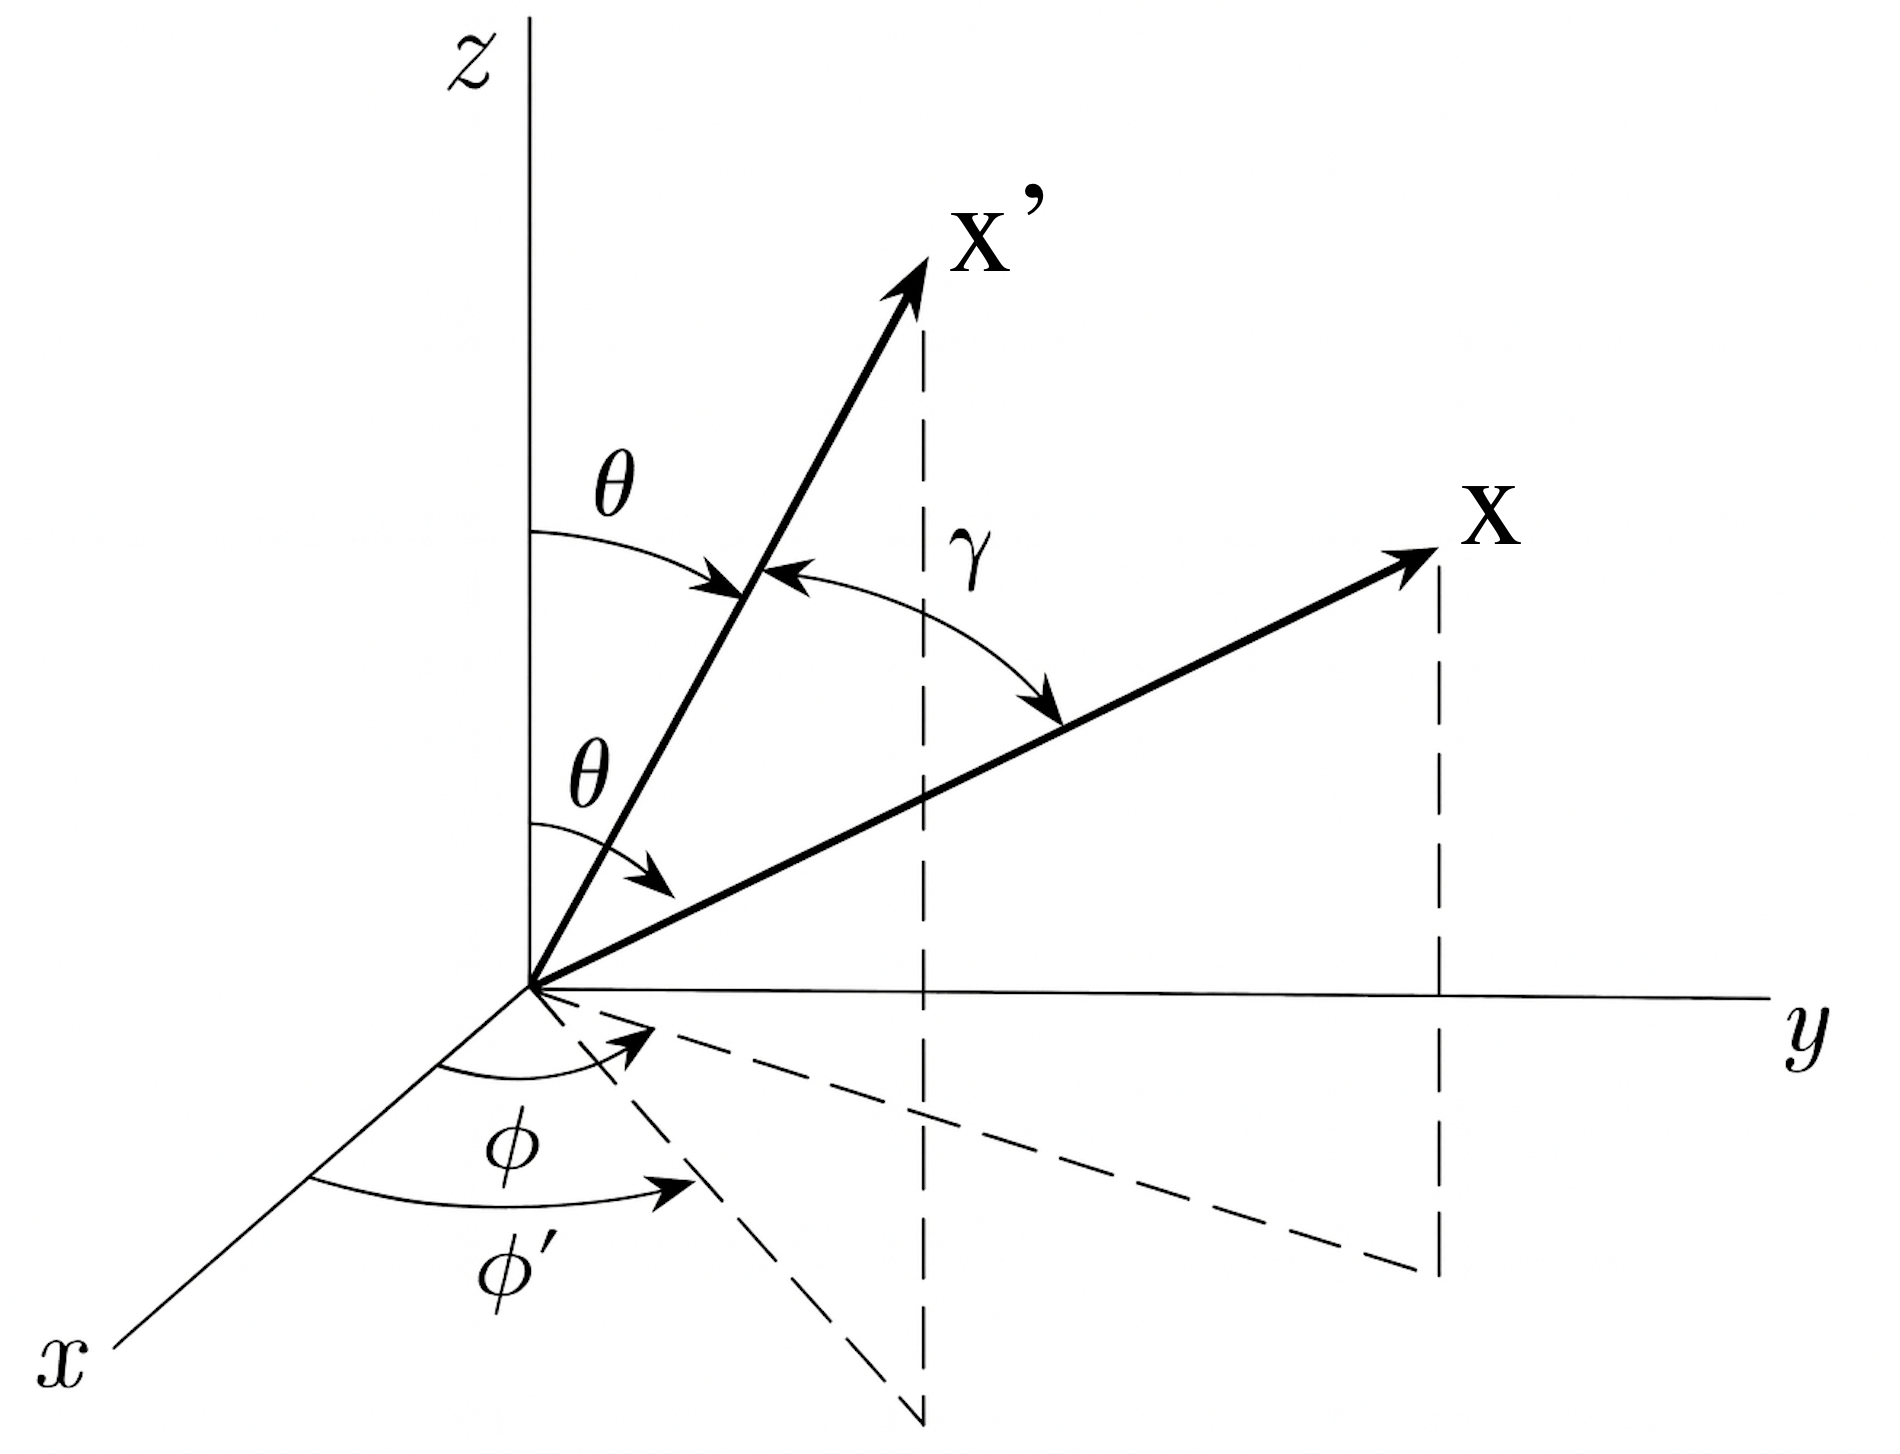
\includegraphics[width=0.5\linewidth]{figure/image29.png}
    \label{fig:chapter_10_1}
\end{figure}

Questo teorema permette di esprimere un polinomio di Legendre di ordine $l$ nell'angolo $\gamma$ in termini di armoniche sferiche negli angoli $\theta , \varphi$ e $\theta' , \varphi'$:

\begin{equation}
    P_l (\cos \gamma) = \frac{4 \pi}{2l +1} \sum_{m=-l} ^l Y_{lm}^* (\theta', \varphi') Y_{lm} (\theta, \varphi)
\end{equation}

Applicando il teorema alla \ref{eq:primo_sviluppo}, otteniamo 

\begin{tcolorbox}[colback=yellow!10!white, colframe=orange!70!black, boxrule=0.8pt]
\begin{equation}
    \frac{1}{|\mathbf{x} - \mathbf{x'}|} = 4 \pi \sum_{l=0}^{\infty} \sum_{m= -l}^{l} \frac{1}{2l +1} \frac{r_<^l}{r_>^{l+1}} Y^*_{lm} (\theta', \varphi') Y(\theta, \varphi) 
    \label{eq:espansione_rapporto_distanza}
\end{equation}
\end{tcolorbox}

\newpage

\section{Multipoli}

Supponiamo di considerare una distribuzione di carica con densità data da $\rho(\mathbf{x'})$. Il potenziale all'esterno di questa distribuzione, grazie a quanto detto prima, può essere espresso mediante uno sviluppo in armoniche sferiche 

\begin{equation}
    V(\mathbf{x}) = \frac{1}{4 \pi \varepsilon_0} \sum_{l = 0}^{\infty} \sum_{m = -l}^l  \frac{4 \pi}{2l +1} q_{lm} \frac{Y_{lm} (\theta , \varphi)}{r^{l +1}}
\end{equation}

dove la particolare scelta dei coefficienti è stata fatta per convenienza. Per risolvere il problema dobbiamo riuscire a determinare i fattori $q_{lm}$. Noi sappiamo che il potenziale di una certa distribuzione con densità $\rho(\mathbf{x})$ è esprimibile con la \ref{eq:potenziale_senza_condizione}, cioè:

\begin{equation*}
    V(\mathbf{x}) = \frac{1}{4 \pi \varepsilon_0} \int_{\tau}\frac{\rho(\mathbf{x})}{|\mathbf{x} - \mathbf{x'}|} d\tau
\end{equation*}

Ma espandendo $1/|\mathbf{x} - \mathbf{x'}|$ come \ref{eq:espansione_rapporto_distanza} otteniamo 

\begin{tcolorbox}[colback=yellow!10!white, colframe=orange!70!black, boxrule=0.8pt]
\begin{equation}
    V(\mathbf{x}) =  \frac{1}{4 \pi \varepsilon_0} \sum_{l = 0}^{\infty} \sum_{m = -l}^l  \frac{4 \pi}{2l +1} \left [ \int Y^*_{lm} (\theta',\varphi') r'^l \rho(\mathbf{x'}) d\tau \right] \frac{Y_{lm} (\theta , \varphi)}{r^{l +1}}
    \label{eq:multipolo_sferiche}
\end{equation}
\end{tcolorbox}

Da questo di capisce che 

\begin{tcolorbox}[colback=yellow!10!white, colframe=orange!70!black, boxrule=0.8pt]
\begin{equation}
    q_{lm} = \int Y^*_{lm} (\theta',\varphi') r'^l \rho(\mathbf{x'}) d\tau 
\end{equation}
\end{tcolorbox}

Questi \mkeyword{momenti di multipolo} coefficienti sono chiamati momenti di multipolo. \\

La \ref{eq:multipolo_sferiche} rappresenta il potenziale quando siamo in coordinate sferiche. In questo caso il calcolo dei momenti di multipolo è meccanico, basta risolvere l'intergrale, tuttavia da questa forma non si intuisce il significato fisico. \\
Per capire meglio il significato fisico è utile passare in coordinate cartesiane:

\begin{tcolorbox}[colback=yellow!10!white, colframe=orange!70!black, boxrule=0.8pt]
\begin{equation}
    V(\mathbf{x}) = \frac{1}{4\pi \varepsilon_0} \left[ \frac{q}{r} + \frac{\mathbf{p} \cdot \mathbf{x}}{r^3} + \frac{1}{2} \sum_{i.j} Q_{ij} \frac{x_i x_j}{r^5} +\  ...\right]
    \label{eq:multipoli_cartesiane}
\end{equation}
\end{tcolorbox}

Dove $q$ è la carica totale del sistema, $\mathbf{p}$ è il momento di dipolo di cui abbiamo parlato nei capitoli precedenti\footnote{Lo sviluppo in multipoli è particolarmente utile (se non necessario) nel caso in cui il sistema considerato sia neutro e il momento di dipolo sia nullo, proprio come anticipato nel capitolo sul dipolo elettrico.}, $Q_{ij}$ è il \mkeyword{tensore momento di quadrupolo} tensore momento di quadrupolo, mentre i puntini indicano la restante parte dello sviluppo, come l'ottupolo, l'esadecopolo etc., che abbiamo deciso di non scrivere in quanto molto lunghi e poiché nella maggior parte dei casi è sufficiente fermarsi al quadrupolo. 

\newpage

\subsection{Quadrupolo}

Vediamo come trovare il potenziale di una una distribuzione quando questa è elettricamente neutra e il momento di dipolo risulta essere nullo. \\

Se ci troviamo in questo caso allora dobbiamo sviluppare il potenziale fino al quadrupolo. Il tensore momento di quadrupolo risulta essere nella forma

\begin{tcolorbox}[colback=yellow!10!white, colframe=orange!70!black, boxrule=0.8pt]
\begin{equation} \label{eq:tensore_quadrupolo}
    Q_{ij} = \int (3x_i' x_j ' - r'^2 \delta_{ij}) \rho (\mathbf{x'}) d^3 x'
\end{equation}
\end{tcolorbox}

Dove con $i$ e $j$ si va ad indicare due delle coordinate $x,y,z$, dell'elemento che si trova in posizione $\mathbf{r'}$. \\
Allora risulta anche che ${(r')^2} = x^2 + y^2 + z^2$.  \\

Questa definizione potrebbe sembrare ancora poco chiara, per questo si riporta anche la formula del tensore momento di dipolo nel caso discreto:

\begin{equation}
    Q_{ij} = \sum_k q_k (3x_i x_j - r^2 \delta_{ij})
\end{equation}

Quindi per trovare il potenziale dobbiamo trovare il valore della matrice 

\begin{equation}
Q = 
\begin{pmatrix}
    Q_{xx} & Q_{xy} & Q_{xz} \\
    Q_{xy} & Q_{yy} & Q_{yz} \\
    Q_{xz} & Q_{yz} & Q_{zz}
\end{pmatrix}
\end{equation}

E sostituire i $Q_{ij}$ nella \ref{eq:multipoli_cartesiane}. \\

Spesso è molto utile andare ad esprimere la densità di carica come combinazione di delta di Dirac su $x,y,z$ e anche come combinazione di funzioni a scalino ($\Theta(x)$). Questo permette di sfruttare le proprietà della delta e semplificare di molto il calcolo degli integrali (che molto spesso hanno valore unitario, proprio grazie alle proprietà delle delta).\footnote{Spiegare questo argomento è più difficile di fare gli esercizi, quindi si consiglia di provare a risolvere qualche esercizio per poi rileggere questa parte di teoria}


\chapter{Dielettrici}

In questo capitolo andremo a trattare come i campi elettrici agiscono sui \emph{mezzi}. \\

I mezzi, ovviamente, si presentano in vari modi (solidi, liquidi, gas, metalli etc.) e le sostanze non rispondono tutte allo stesso modo a un campo elettrico. Tuttavia la \emph{maggio parte} degli oggetti appartiene a una di queste due grandi famiglie: \emph{conduttori} e \emph{isolanti} (o \emph{dielettrici}) \mkeyword{dielettrici}. Nei capitoli precedenti abbiamo già trattato dei conduttori; queste sono sostanze in cui le cariche sono libere di muoversi. \\

Nei dielettrici, al contrario, \emph{tutte le cariche sono legate a specifici atomi e molecole} e il massimo che possono fare è muoversi di poco \emph{ entro } questi. \\

Esistono in realtà due meccanismi principali attraverso i quali i campi elettrici possono distorcere la distribuzione di carica di un atomo o di una molecola dielettrica: stiramento e rotazione.\\
In ognuno di questi casi il momento di dipolo di ciascuna molecola sarà modificato rispetto a quello che si avrebbe in assenza del campo. 

\begin{figure} [h]
    \centering
    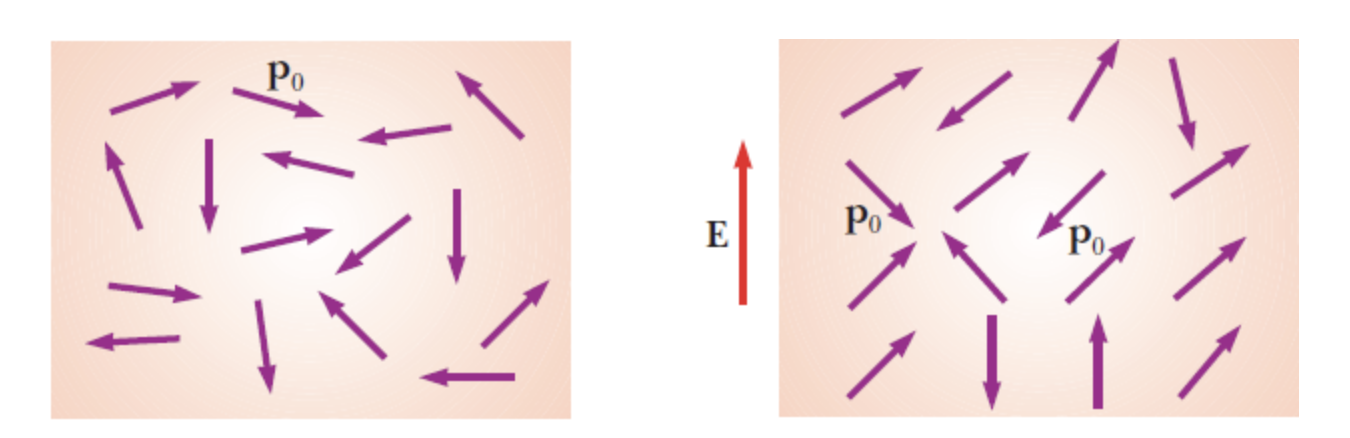
\includegraphics[width=0.8\linewidth]{figure/image23.png}
    \caption{Azione del campo elettrostatico sulle molecole di una sostanza dotate di momento di dipolo intrinseco}
    \label{fig:chapter_11_1}
\end{figure}

Allora possiamo andare ad ipotizzare che ciascuna molecola acquisti un \emph{momento di dipolo medio} $< \mathbf{p} >$ microscopico \emph{parallelo} al campo elettrostatico $\mathbf{E}$. \\

Considerato un volumetto $\Delta \tau$ del dielettrico, contenente $\Delta N$ atomi (o molecole), il momento di dipolo risultante è dato dal prodotto $\Delta N  <\mathbf{p}>$ e il momento di dipolo elettrico per unità di volume è dato da 

\begin{equation}
    \mathbf{P} = \frac{\Delta N}{\Delta \tau} < \mathbf{p} >
\end{equation}

Il \mkeyword{polarizzazione del dielettrico} vettore $\mathbf{P}$ che caratterizza l'effetto di formazione dei momenti di dipolo indotti dal campo esterno, si chiama \emph{polarizzazione del dielettrico}.\\
In particolare se facciamo tendere $\Delta \tau$ a zero, otteniamo il valore di $\mathbf{P}$ in uno specifico punto del dielettrico. \\

\newpage

Esiste un'importante tipologia di dielettrici che prende \mkeyword{dielettrici lineari} il nome di dielettrici \emph{lineari}.\\ 
Un dielettrico lineare è un materiale in cui la \emph{polarizzazione $\mathbf{P}$ è proporzionale al campo elettrico applicato $\mathbf{E}$}, in particolare:

\begin{tcolorbox}[colback=yellow!10!white, colframe=orange!70!black, boxrule=0.8pt]
\begin{equation}
    \mathbf{P} = \varepsilon_0 (\kappa_e - 1) \mathbf{E} = \varepsilon_0 \chi_e \mathbf{E}
\end{equation}
\end{tcolorbox}

Dove $\kappa_e$ prende il \mkeyword{costante dielettrica relativa del dielettrico} nome di \emph{costante dielettrica relativa del dielettrico}, mentre $\chi_e$ prende il nome di \mkeyword{suscettività elettrica del dielettrico}  \emph{suscettività elettrica del dielettrico}.\\
Queste due grandezze \emph{dipendono solamente dalla natura del dielettrico, indipendentemente dalla geometria e grandezza}.\\

Per il resto del capitolo \emph{andiamo a ipotizzare che i dielettrici considerati siano lineari}.\\

\' E possibile fare un'ulteriore suddivisione tra i dielettrici: \emph{isotropi} e \emph{anisotropi}. \\

Un dielettrico è isotropo quando la sua polarizzazione in ogni punto è parallela al campo elettrico $\mathbf{E}$, cioè quando $\chi_e$ è uno scalare. \\

\' E anisotropo quando la sua polarizzazione non è parallela al campo e $\chi_e$ è un 2-tensore (una matrice 3x3). \\

\section{Campo elettrico prodotto da un dielettrico polarizzato}

Supponiamo di avere un dielettrico soggetto a un campo elettrico, per quanto visto sopra il momento di dipolo di ciascuna molecola sarà modificato, questo comporta che \emph{il dielettrico stesso genera un campo elettrico}.\\

Andiamo a trovare il campo elettrico generato dal dielettrico. Per semplicità di calcolo ricaviamo il potenziale (cosa che ci porta a conoscere anche il campo).\\

Possiamo andare a suddividere il dielettrico in un numero infinito di parti, ciascuna delle quali rappresenta un dipolo.\\ Per ogni parte vale

\begin{equation*}
    V(\mathbf{r}) = \frac{1}{4 \pi \varepsilon_0} \frac{\mathbf{p} \cdot \mathbf{u}_r}{r^2}
\end{equation*}

dove $\mathbf{r}$ è il vettore che va dal dipolo al punto nello spazio dove vogliamo trovare il potenziale. \\

Per come abbiamo definito $\mathbf{P}$, possiamo affermare che $\mathbf{p} = \mathbf{P} d\tau'$ in tutti gli infinitesimi volumi $d \tau '$ in cui abbiamo diviso il materiale.\footnote{con " ' " si va a indicare che quella grandezza si riferisce al particolare punto del dielettrico} \\

Allora tutto il potenziale in un punto risulta essere 

\begin{equation}
    V(\mathbf{r}) = \frac{1}{4 \pi \varepsilon_0} \int_{\tau} \frac{\mathbf{P}(\mathbf{r'}) \cdot \mathbf{u}_r}{r^2} \ d \tau '
\end{equation}

In principio questo basterebbe, ma possiamo fare un'importante osservazione 

\begin{equation}
    \nabla \left(\frac{1}{r} \right) = \frac{\mathbf{u}_r}{r^2}
\end{equation}

Quindi

\begin{equation*}
    V = \frac{1}{4 \pi \varepsilon_0} \int_{\tau} \mathbf{P} \cdot \nabla \left(\frac{1}{r} \right) \ d\tau '
\end{equation*}

Sappiamo che vale 

\begin{equation*}
    \mathbf{P} \cdot \nabla \left(\frac{1}{r} \right) = \nabla \cdot \left(\frac{\mathbf{P}}{r} \right) - \frac{1}{r} \ (\nabla \cdot \mathbf{P})
\end{equation*}

Allora sostituendo

\begin{equation*}
     V = \frac{1}{4 \pi \varepsilon_0} \left [ \int_{\tau}  \nabla \cdot \left(\frac{\mathbf{P}}{r} \right) \ d\tau ' - \int_{\tau} \frac{1}{r} (\nabla \cdot \mathbf{P}) \ d \tau '\right ]
\end{equation*}

Applicando il teorema della divergenza 

\begin{tcolorbox}[colback=yellow!10!white, colframe=orange!70!black, boxrule=0.8pt]
\begin{equation}
         V = \frac{1}{4 \pi \varepsilon_0}  \oint_{\Sigma}  \frac{\mathbf{1}}{r} \ \mathbf{P} \cdot \mathbf{\hat{n}} \ d\Sigma ' - \frac{1}{4 \pi \varepsilon_0} \int_{\tau} \frac{1}{r} (\nabla \cdot \mathbf{P}) \ d \tau '
\end{equation}
\end{tcolorbox}

Si nota che il primo termine sembra molto il potenziale di una superficie di carica 

\begin{tcolorbox}[colback=yellow!10!white, colframe=orange!70!black, boxrule=0.8pt]
\begin{equation}
    \sigma_p \equiv \mathbf{P} \cdot \mathbf{\hat{n}}
\end{equation}
\end{tcolorbox}

Dove $\sigma_p$ è la \mkeyword{densità superficiale delle cariche polarizzate} \emph{densità superficiale delle cariche polarizzate}, mentre $\mathbf{\hat{n}}$ è il versore tangente alla superficie del dielettrico e \emph{uscente} da questa. \\

Mentre il secondo termine assomiglia a un potenziale di volume di carica 

\begin{tcolorbox}[colback=yellow!10!white, colframe=orange!70!black, boxrule=0.8pt]
\begin{equation}
    \rho_p \equiv - \nabla \cdot \mathbf{P}
\end{equation}
\end{tcolorbox}

Dove \mkeyword{densità volumica delle cariche polarizzate} $\rho_p$ è la \emph{densità volumica delle cariche polarizzate}.\\

\newpage

\subsection{Interpretazione fisica delle cariche di polarizzazione}

Queste cariche potrebbero sembrare "fittizie" - semplici strumenti per facilitare il calcolo dei campi. Tuttavia non è così, $\rho_p $ e $ \sigma_p$ rappresentano accumuli di carica perfettamente autentici. \\

L'idea di base è molto semplice: supponiamo che la polarizzazione $\mathbf{P}$ sia uniforme, e supponiamo di avere una lunga serie di dipoli.

\begin{figure}[h]
    \centering
    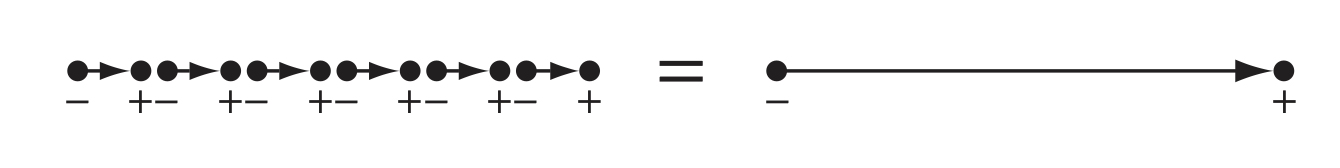
\includegraphics[width=0.65\linewidth]{figure/image24.png}
    \caption{Linea di dipoli}
    \label{fig:chapter_11_2}
\end{figure}

La testa di uno annulla di fatto la coda del
suo vicino, ma alle estremità rimangono due cariche: $+$ all'estremità destra e $-$ a quella sinistra. È come se avessimo staccato un elettrone da un'estremità e lo avessimo portato
fino all'altra estremità, anche se in realtà nessun singolo elettrone ha percorso
l'intero percorso: molti piccoli spostamenti si sommano per formare un unico grande spostamento.\\

Se la polarizzazione è non uniforme, otteniamo un accumulo di cariche anche all'\emph{interno} del materiale oltre che sulla superficie (le cariche dei dipoli il linea non si annullano sovrapponendosi).

\section{Equazioni dell'elettrostatica in presenza di dielettrici}

Dal momento che il campo prodotto da cariche elettriche è conservativo anche in presenza di dielettrici polarizzati, continuano a valere le due condizioni, integrale e locale, date da

\begin{equation*}
    \oint \mathbf{E} \cdot d \mathbf{s} = 0 \quad , \quad  \nabla \times \mathbf{E} = 0
\end{equation*}

e la proprietà equivalente che il campo elettrostatico si possa ottenere come gradiente della funzione potenziale, $\mathbf{E} = - \nabla V$. \\

Anche la legge di Gauss resta valida in presenza di dielettrici polarizzati, \emph{purché si tenga conto delle cariche di polarizzazione oltre che delle cariche libere}:

\begin{tcolorbox}[colback=yellow!10!white, colframe=orange!70!black, boxrule=0.8pt]
\begin{equation}
    \oint_{\Sigma} \mathbf{E} \cdot \mathbf{u}_n \ d \Sigma = \frac{q + q_p}{\varepsilon_0}
\end{equation}
\end{tcolorbox}

Deduciamo la forma locale 

\begin{tcolorbox}[colback=yellow!10!white, colframe=orange!70!black, boxrule=0.8pt]
\begin{equation}
    \nabla \cdot \mathbf{E} = \frac{\rho + \rho_p}{\varepsilon_0}
\end{equation}
\end{tcolorbox}

\newpage

Allora, si nota facilmente che 

\begin{equation}
    \varepsilon_0 \nabla \cdot \mathbf{E} = \nabla \cdot \varepsilon_0 \mathbf{E} = \rho - \nabla \cdot \mathbf{P} \implies \nabla \cdot (\varepsilon_0 \mathbf{E} + \mathbf{P}) = \rho
\end{equation}

a cui corrisponde l'integrale 

\begin{equation}
    \oint_{\Sigma} (\varepsilon_0 \mathbf{E} + \mathbf{P}) \cdot \mathbf{u}_n \ d \Sigma = q
\end{equation}

Allora possiamo andare a definire una nuova grandezza vettoriale 

\begin{tcolorbox}[colback=yellow!10!white, colframe=orange!70!black, boxrule=0.8pt]
\begin{equation}
    \mathbf{D} = \varepsilon_0 \mathbf{E} + \mathbf{P}
\end{equation}
\end{tcolorbox}

Dove $\mathbf{D}$ prende \mkeyword{induzione dielettrica} il nome di \emph{induzione dielettrica}. \\

Allora possiamo scrivere:

\begin{tcolorbox}[colback=yellow!10!white, colframe=orange!70!black, boxrule=0.8pt]
\begin{equation}
    \nabla \cdot \mathbf{D} = \rho \quad , \quad \oint_{\Sigma} \mathbf{D} \cdot \mathbf{u}_n \ d \Sigma = q
\end{equation}
\end{tcolorbox}

Il flusso del vettore induzione dielettrica $\mathbf{D}$ attraverso una superficie chiusa, contenente in generale sia cariche libere che cariche polarizzate, \emph{dipende soltanto dalle cariche libere}. \\

Per completezza aggiungiamo che per il vettore induzione dielettrica non si può stabilire che la circuitazione lungo qualsiasi percorso chiuso è nulla: $\mathbf{D}$ non è cioè un campo conservativo. \\

\subsection{Relazioni per dielettrici lineari}

Dato che stiamo trattando dielettrici lineari, è possibile travare una relazione diretta tra $\mathbf{D}$ e $\mathbf{E}$ e tra $\mathbf{D}$ e $\mathbf{P}$. Sostituendo

\begin{equation*}
    \mathbf{P} = \varepsilon_0 (\kappa_e - 1) \mathbf{E} = \varepsilon_0 \chi_e \mathbf{E}
\end{equation*}

nella definizione di induzione elettrica si ottengono le seguenti relazioni:

\begin{tcolorbox}[colback=yellow!10!white, colframe=orange!70!black, boxrule=0.8pt]
\begin{equation}
    \mathbf{D} = \varepsilon_0 \kappa_e \mathbf{E} = \varepsilon \mathbf{E}
    \label{eq:legame_D_E}
\end{equation}
\end{tcolorbox}

Dove \mkeyword{costante dielettrica assoluta} $\varepsilon$ è definito come il prodotto tra $\varepsilon_0$ e $\kappa_e$ e prende il nome di costante dielettrica assoluta del dielettrico. 

\begin{tcolorbox}[colback=yellow!10!white, colframe=orange!70!black, boxrule=0.8pt]
\begin{equation}
    \mathbf{P} = \frac{\kappa_e - 1}{\kappa_e} \mathbf{D} = \frac{\chi_e}{1 + \chi_e} \mathbf{D}
\end{equation}
\end{tcolorbox}

\newpage

In particolare si ottiene che $\nabla \cdot \mathbf{P} \propto \nabla \cdot \mathbf{D}$, quindi se $\nabla \cdot \mathbf{D} = 0$ vale che 

\begin{equation}
    \rho_p = - \nabla \cdot \mathbf{P} = 0  
\end{equation}

Cioè in un dielettrico lineare e omogeneo la densità spaziale di carica di polarizzazione è nulla e le cariche di polarizzazione sono distribuite esclusivamente sulle superfici.  

\section{Discontinuità dei campi sulla superficie di separazione tra due dielettrici}

Andiamo a vedere come si comporta un campo elettrostatico quando attraversa una superficie di separazione tra due dielettrici con costante dielettrica diversa. \\

Supponiamo di avere due dielettrici con costante dielettrica relativa $\kappa_{e_1}$ e $\kappa_{e_2}$ e sia $\Sigma$ la superficie di separazione. Indichiamo con $\mathbf{E}_1$, $\mathbf{P}_1$ , $\mathbf{D}_1$ rispettivamente il campo elettrostatico, la polarizzazione e l'induzione dielettrica sulla faccia di $\Sigma$ rivolta al dielettrico di costante dielettrica $\kappa_{e_1}$  e con $\mathbf{E}_2$, $\mathbf{P}_2$ , $\mathbf{D}_2$ i corrispettivi valori sulla faccia di $\Sigma$ rivolta al secondo dielettrico. \\

\begin{figure}[h]
    \centering
    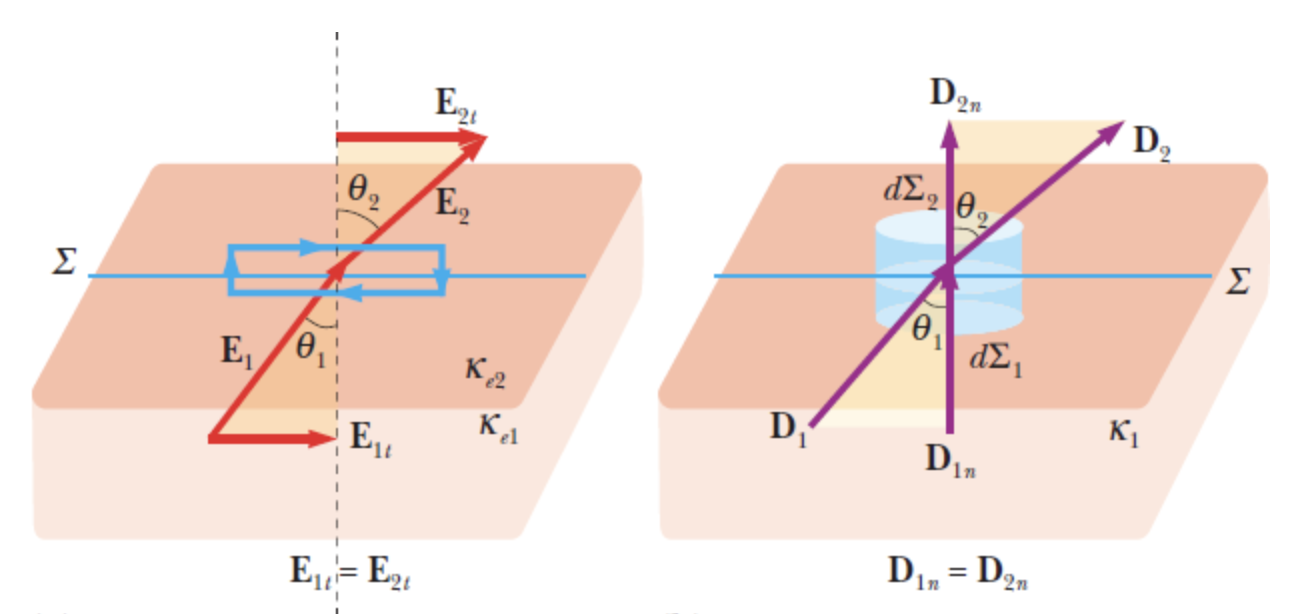
\includegraphics[width=0.7\linewidth]{figure/image25.png}
    \caption{}
    \label{fig:dielettrici_mezzi}
\end{figure}

Vediamo cosa succede alla componente tangenziale al piano del campo elettrico nel passaggio attraverso $\Sigma$.\\

Consideriamo una linea chiusa rettangolare che attraversa $\Sigma$ e in cui la lunghezza dei lati perpendicolari alla superficie è molto minore della lunghezza dei lati paralleli (come in Figura \ref{fig:dielettrici_mezzi}). Essendo entrambi i campi elettrici conservati, deve valere

\begin{equation}
    \oint \mathbf{E} \cdot d \mathbf{s} = 0 \implies E_{1t} \ l - E_{1t} \ l = 0
\end{equation}

Nella relazione abbiamo approssimati i lati perpendicolari. Allora otteniamo 

\begin{tcolorbox}[colback=yellow!10!white, colframe=orange!70!black, boxrule=0.8pt]
\begin{equation}
    E_{1t} = E_1 \sin \theta_1 = E_2 \sin \theta_2 = E_{2t}
\end{equation}
\end{tcolorbox}

Cioè la componente tangenziale di $\mathbf{E}$ rimane costante nel passaggio attraverso $\Sigma$. \\


Applichiamo adesso la legge di Gauss al vettore $\mathbf{D}$, scegliendo per superficie chiusa di integrazione una scatola cilindrica di altezza infinitesima ortogonale a $\Sigma$ e con le basi $d \Sigma_1$ di normali $\mathbf{u}_{n_1}$ e $d \Sigma_2$ di normale $\mathbf{u}_{n_2}$ all'interno dei due dielettrici. 

\begin{equation}
    \oint_{\Sigma'} \mathbf{D} \cdot \mathbf{u}_n ' \ d \Sigma ' = \mathbf{D}_2 \cdot \mathbf{u}_{n_2} \ d \Sigma + \mathbf{D}_1 \cdot \mathbf{u}_{n_1} \ d \Sigma = (D_{2n} - D_{1n}) d\Sigma = 0 
\end{equation}

Ma allora vale che 

\begin{tcolorbox}[colback=yellow!10!white, colframe=orange!70!black, boxrule=0.8pt]
\begin{equation}
    D_{1n} = D_{2n}
\end{equation}
\end{tcolorbox}

Inoltre dalla relazione \ref{eq:legame_D_E} otteniamo:

\begin{tcolorbox}[colback=yellow!10!white, colframe=orange!70!black, boxrule=0.8pt]
\begin{equation}
    \kappa_{e_1} \varepsilon_0 E_1 \cos \theta_1 = \kappa_{e_2} \varepsilon_0 E_2 \cos \theta_2
\end{equation}
\end{tcolorbox}

E dividendo membro a membro 

\begin{tcolorbox}[colback=yellow!10!white, colframe=orange!70!black, boxrule=0.8pt]
\begin{equation}
    \frac{\text{tg} \theta_1}{\text{tg} \theta_2} = \frac{\kappa_{e_1}}{\kappa_{e_2}}
\end{equation}
\end{tcolorbox}

La discontinuità della componente normale di $\mathbf{E}$, insieme alla continuità della componente tangenziale, comporta un cambiamento di direzione delle linee di forza del campo elettrostatico. 

\newpage

\subsection{Problemi al contorno con i dielettrici}
I metodi usati nei capitoli precedenti per la soluzione di problemi di valori al contorno possono essere facilmente applicati anche in presenza di dielettrici. In questo paragrafo tratteremo alcuni esempi delle varie tecniche applicate a mezzi dielettrici. 

\subsubsection{Carica entro un dielettrico semi-infinito}

Consideriamo una carica puntiforme $q$ disposta entro un dielettrico semi-infinito di costante dielettrica \emph{assoluta} $\varepsilon_1$ ad una distanza $d$ dal piano di separazione del primo mezzo da un secondo dielettrico dielettrico semi-infinito di costante $\varepsilon_2$. Il piano di separazione sia il piano $z = 0$. 

\begin{figure}[h]
    \centering
    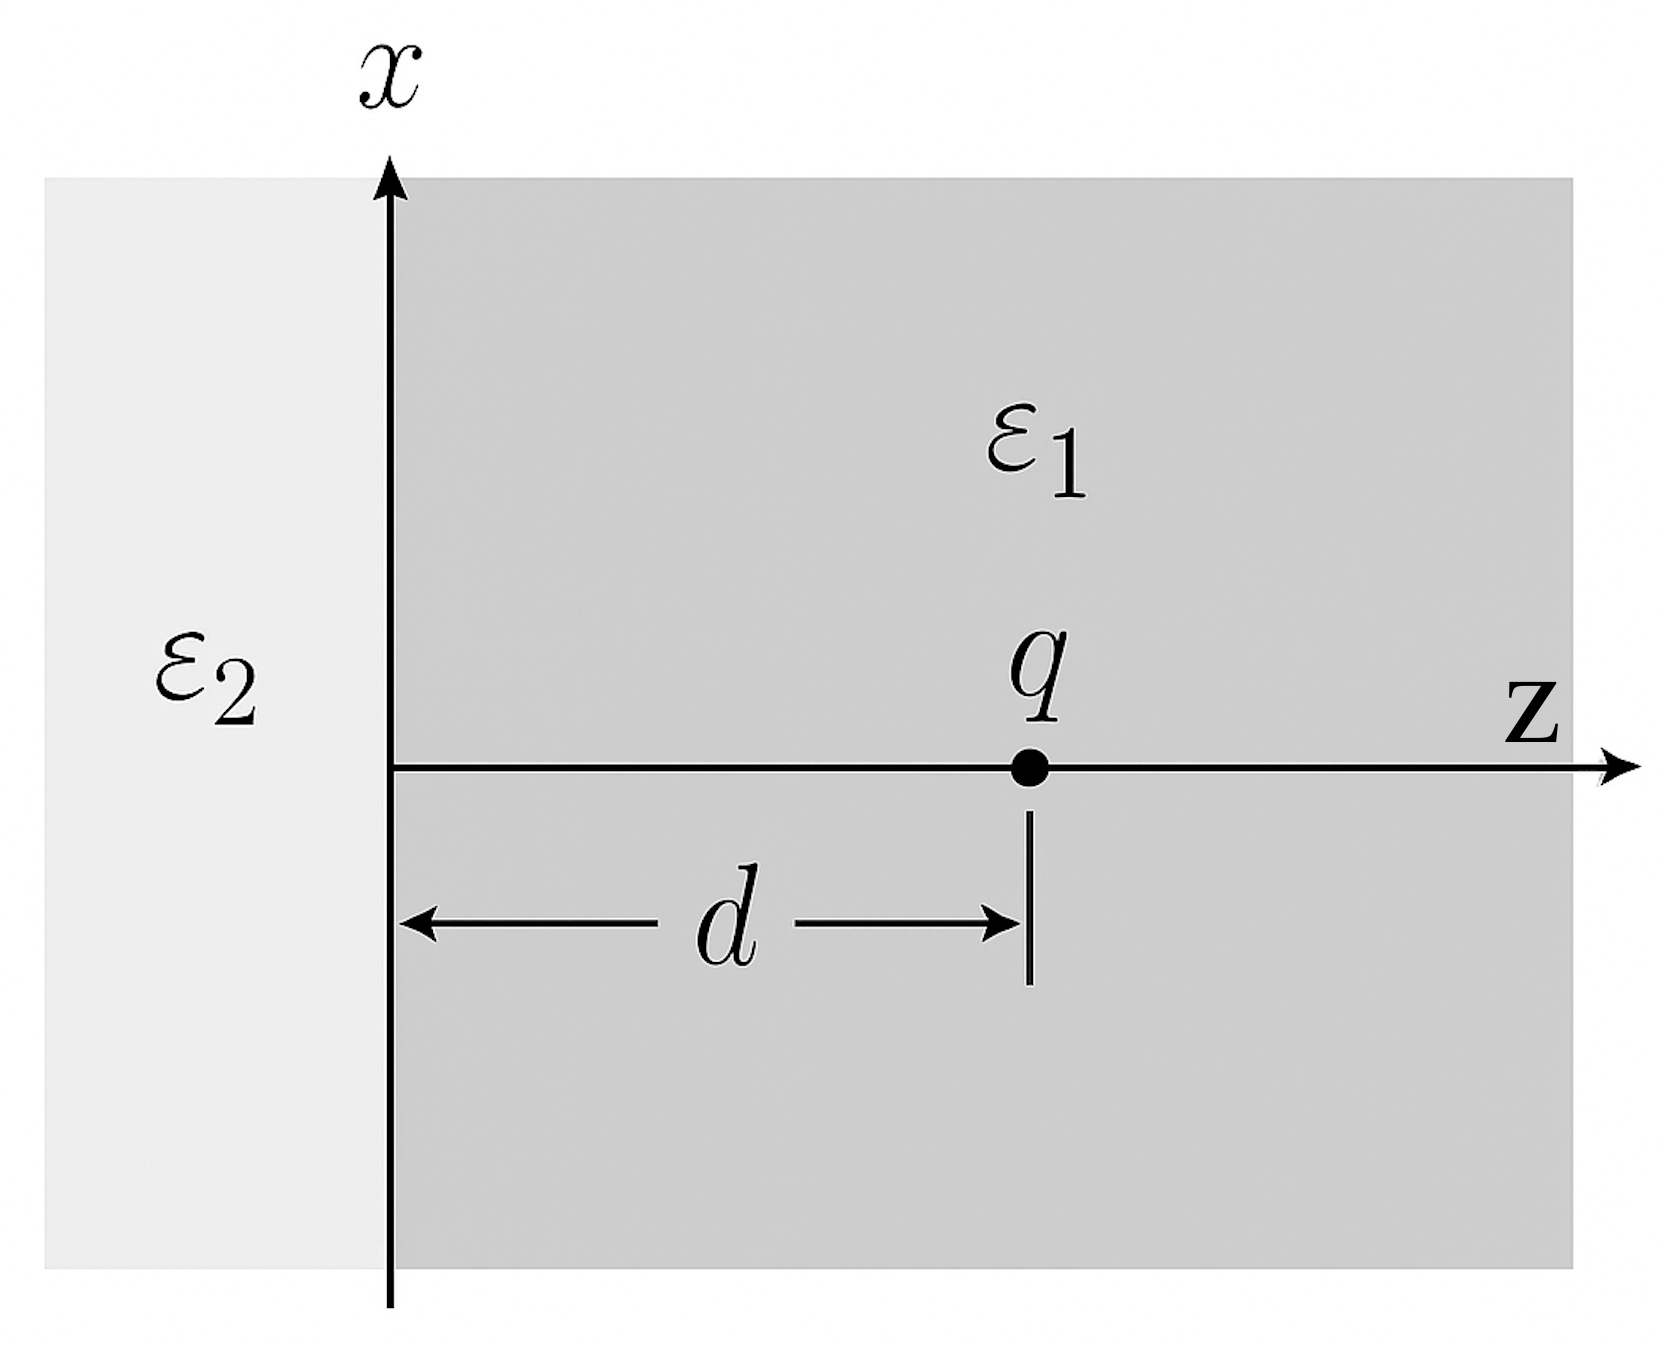
\includegraphics[width=0.35\linewidth]{figure/image26.png}
    \caption{Dielettrici semi-infiniti}
    \label{fig:chapter_11_3}
\end{figure}

Dobbiamo trovare una soluzione appropriata per le condizioni

\begin{align*}
    \varepsilon_1 \nabla \cdot E = \rho \quad  \quad z >0\\
    \varepsilon_2 \nabla \cdot E = 0 \quad  \quad z <0
\end{align*}

Le condizioni al contorno per $z = 0$ sono :

\begin{equation}
    \lim_{z \to 0^{+}} \colvec{ \varepsilon_1 E_z \\ E_x \\ E_y} = \lim_{z \to 0^{-}} \colvec{ \varepsilon_2 E_z \\ E_x \\ E_y}
    \label{eq:condizioni_dipoli}
\end{equation}

Volendo usare il metodo delle cariche immagine per trovare il potenziale nel semispazio contenente la carica, appare naturale disporre una carica immagine $q'$ posta nella posizione simmetrica $A'$ rispetto alla posizione $A$ della carica $q$. 

\begin{figure}[h]
    \centering
    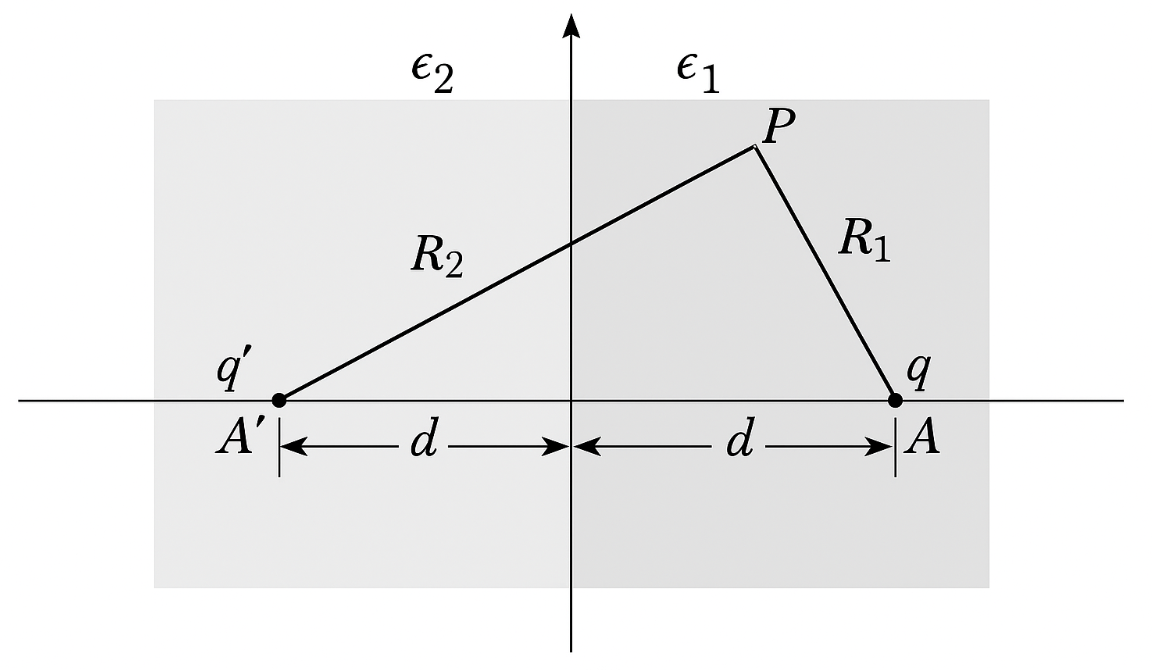
\includegraphics[width=0.55\linewidth]{figure/image27.png}
    \caption{}
    \label{fig:chapter_11_4}
\end{figure}

\newpage

Allora per $z > 0$ il potenziale nel punto $P$ di coordinate cilindriche $(\rho, \theta,z)$ sarà 

\begin{equation}
    V(\rho, \theta, z) = \frac{1}{4 \pi \varepsilon_1} \left( \frac{q}{R_1} + \frac{q'}{R_2} \right) \qquad z >0
\end{equation}

dove $R_1 = \sqrt{\rho^2 + (d-z)^2}$ e $R_2 = \sqrt{\rho^2 + (d + z)^2}$. \\

Ora dobbiamo trovare il potenziale per $z<0$. Siccome in questo semispazio non ci sono cariche, il potenziale deve essere soluzione della equazione di Laplace senza singolarità. L'ipotesi più semplice è evidentemente che per $z<0$ il potenziale sia equivalente a quello di una carica $q''$ nella posizione $A$ della carica effettiva q:

\begin{equation}
    V(\rho, \theta, z) = \frac{1}{4 \pi \varepsilon_2} \frac{q''}{R_1} \qquad z<0
\end{equation}

Dato che 

\begin{equation*}
    \frac{\partial}{\partial z} \left ( \frac{1}{R_1} \right)_{z = 0} = -\frac{\partial}{\partial z} \left ( \frac{1}{R_2} \right)_{z = 0} = \frac{d}{(\rho^2 + d^2)^{3/2}}
\end{equation*}

Mentre

\begin{equation*}
    \frac{\partial}{\partial \rho} \left ( \frac{1}{R_1} \right)_{z = 0} = \frac{\partial}{\partial \rho} \left ( \frac{1}{R_2} \right)_{z = 0} = - \frac{\rho}{(\rho^2 + d^2)^{3/2}}
\end{equation*}

Allora dalle condizioni al bordo \ref{eq:condizioni_dipoli} otteniamo

\begin{equation}
    \begin{cases}
        q-q' = q''\\
        \frac{1}{\varepsilon_1} (q + q') = \frac{1}{\varepsilon_2} q''
    \end{cases}
\end{equation}

Risolvendo il sistema si ottiene che 

\begin{tcolorbox}[colback=yellow!10!white, colframe=orange!70!black, boxrule=0.8pt]
\begin{equation}
    q' = -\left( \frac{\varepsilon_2 - \varepsilon_1}{\varepsilon_2 + \varepsilon_1} \right) q \quad ,  \quad q'' = \left( \frac{2 \varepsilon_2}{\varepsilon_2 + \varepsilon_1} \right)
\end{equation}
\end{tcolorbox}

\subsubsection{Sfera dielettrica in campo uniforme}

Consideriamo una sfera di dielettrico di raggio $a$ con costante dielettrica relativa $\varepsilon/\varepsilon_0$, soggetta a un campo elettrostatico uniforme.

\begin{figure} [h]
    \centering
    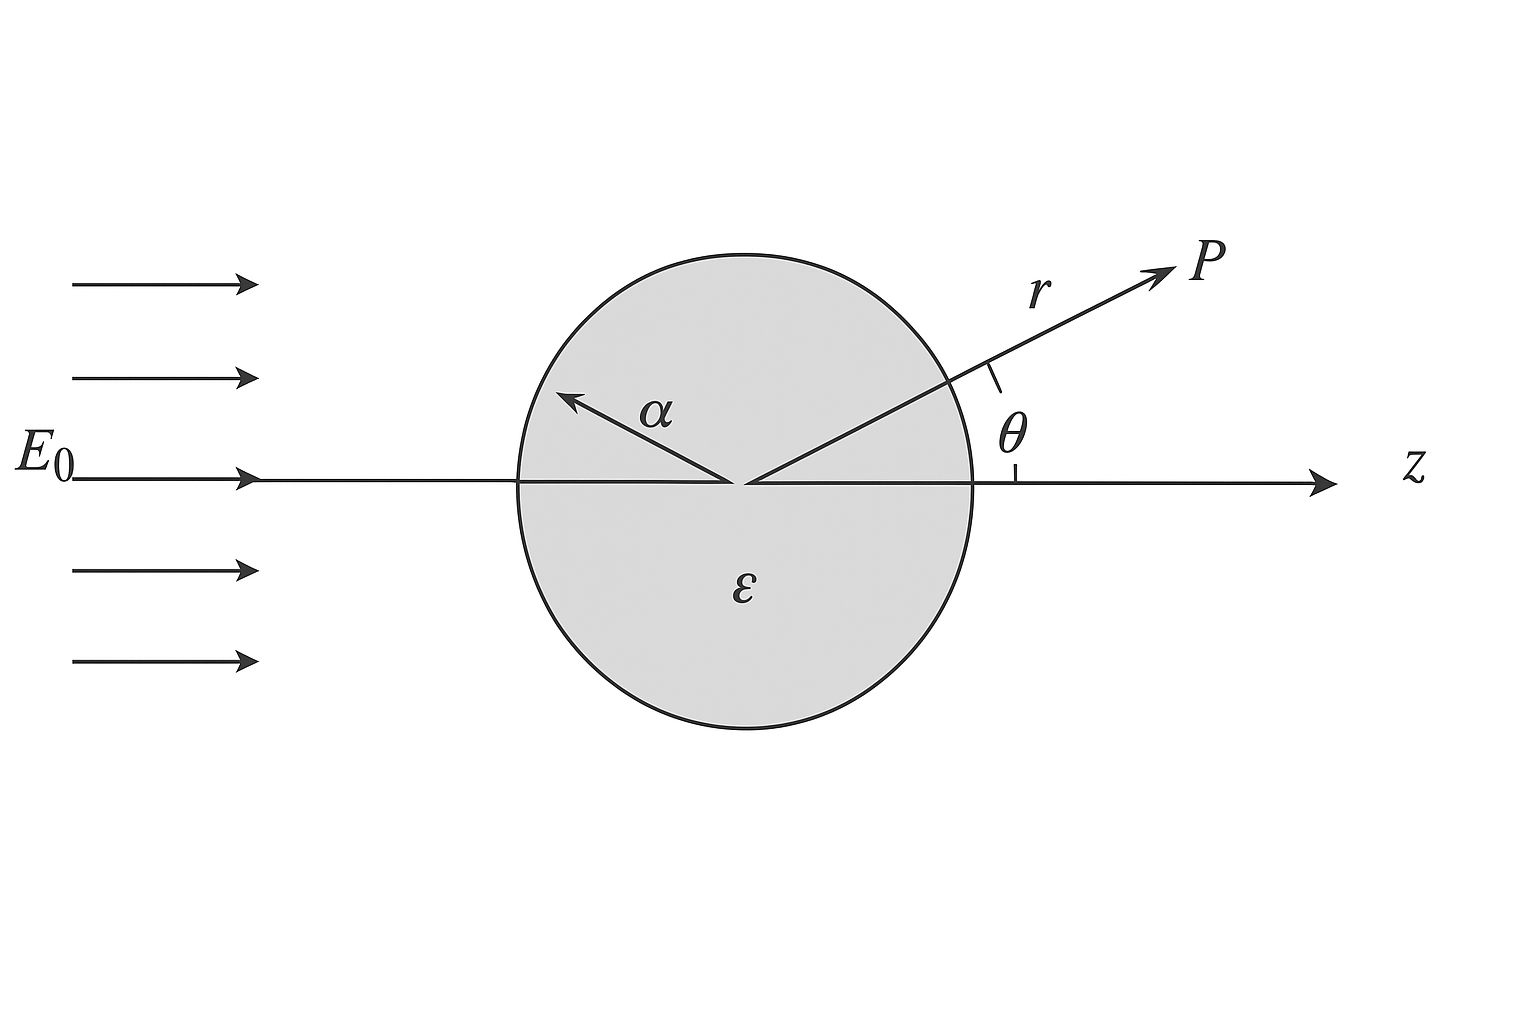
\includegraphics[width=0.5\linewidth]{figure/image28.png}
    \caption{Sfera di dielettrico in campo uniforme}
    \label{fig:chapter_11_5}
\end{figure}

Applicando il metodo di separazione delle variabili e sfruttando la simmetria azimutale del sistema, possiamo sapere la forma del potenziale all'interno e all'esterno della sfera:

\begin{equation}
    V_{in} (r, \theta) = \sum_{l= 0}^{+ \infty} A_l r^l P_l (\cos \theta) \qquad , \qquad V_{est}(r, \theta) = \sum_{l = 0} ^ {+ \infty} \left ( B_l r^l + C_l \frac{1}{r^{l+1}} \right) P_l (\cos \theta)
\end{equation}

Si sottolinea il fatto che nel potenziale all'interno della sfera i coefficienti dei termini $1/r^{l+1}$ sono nulla in quanto all'interno della sfera è contenuta anche l'origine del sistema. \\

Andiamo ad imporre le condizioni al contorno per trovare il valore dei coefficienti. \\

Dalla condizione all'infinito ($V \to - E_0 z = - E_0 \cos \theta$) si trova che l'unico coefficiente $B_l$ che non si annulla è $B_1 = -E_0$.\\

Gli altri coefficienti si trovano grazie alle condizioni al contorno per $r = a$:\\

La condizione tangenziale alla superficie

\begin{align*}
    - \frac{1}{a} \frac{\partial V_{in}}{\partial \theta} _{r= a} = - \frac{1}{a} \frac{\partial V_{est}}{\partial \theta} _{r= a}\\
\end{align*}

La condizione normale alla superficie

\begin{equation*}
    -\varepsilon \frac{\partial V_{in}}{\partial r} _{r = a} =  -\varepsilon \frac{\partial V_{est}}{\partial r} _{r = a} \quad
\end{equation*}

Una volta fatta la sostituzione si ottengono due serie di funzioni di Legendre uguali a zero. Dato che si devono annullare per qualsiasi $\theta$, i coefficienti di ciascuna funzione di Legendre deve annullarsi separatamente. Si ottengono le seguenti condizioni:

\begin{equation}
    \begin{cases}
        A_1 = - E_0 + \frac{C_1}{a^3} \\
        A_l = \frac{C_l}{a^{2l +1}} \quad  l\neq 1\\
        (\varepsilon/\varepsilon_0) A_1 = - E_0 - 2 \frac{C_1}{a^3}\\
        (\varepsilon/\varepsilon_0) l A_l = - (l+1) \frac{C_l}{a^{2l +1}} \quad l\neq 1
    \end{cases}
\end{equation}

Le condizioni riguardanti le $l$ possono essere soddisfatte contemporaneamente se e solo se $A_l = C_l = 0$ per $l \neq 1$. Allora risulta

\begin{align}
    A_l = - \left ( \frac{3}{2 + \varepsilon/\varepsilon_0} \right) E_0\\
    C_l = \left( \frac{\varepsilon/\varepsilon_0 - 1}{\varepsilon/\varepsilon_0 + 2} \right) a^3 E_0
\end{align}

\newpage

Allora i potenziali diventano 

\begin{tcolorbox}[colback=yellow!10!white, colframe=orange!70!black, boxrule=0.8pt]
\begin{align}
    V_{in} (r, \theta) = - \left ( \frac{3}{2 + \varepsilon/\varepsilon_0} \right) E_0 \ r \cos \theta\\
    V_{est} (r, \theta) = - E_0 r \cos \theta + \left( \frac{\varepsilon/\varepsilon_0 - 1}{\varepsilon/\varepsilon_0 + 2} \right) E_0 \frac{a^3}{r^2} \cos \theta
\end{align}
\end{tcolorbox}

Si nota allora che al di fuori della sfera sfera il potenziale è equivalente al potenziale dovuto al campo uniforme $E_0$ e al campo di un dipolo posto nell'origine con momenti di dipolo:

\begin{tcolorbox}[colback=yellow!10!white, colframe=orange!70!black, boxrule=0.8pt]
\begin{equation}
    p = 4 \pi \varepsilon_0 \left( \frac{\varepsilon/\varepsilon_0 - 1}{\varepsilon/\varepsilon_0 + 2} \right) a^3 E_0
\end{equation}
\end{tcolorbox}

Questo momento di dipolo può essere interpretato come l'integrale di volume della polarizzazione $\mathbf{P}$, quindi risulta 

\begin{tcolorbox}[colback=yellow!10!white, colframe=orange!70!black, boxrule=0.8pt]
\begin{equation}
    \mathbf{P} = 3 \varepsilon_0 \left( \frac{\varepsilon/\varepsilon_0 - 1}{\varepsilon/\varepsilon_0 + 2} \right)  \mathbf{E}_0
\end{equation}
\end{tcolorbox}

\section{Energia elettrostatica nei dielettrici}

Consideriamo un sistema formato da un dielettrico e da delle cariche libere e vogliamo trovare l'energia elettrostatica di tale sistema. \\

Supponiamo di considerare il dielettrico fisso nello spazio e di aggiungere una alla volta le cariche libere. Con l'aumentare la densità delle cariche libere $\rho$ di una quantità $\Delta \rho$, cambierà anche la densità di polarizzazione del dielettrico; tuttavia, noi siamo interessati solo nel lavoro svolto per aumentare le cariche \emph{libere}:

\begin{equation}
    \Delta W  = \int (\Delta \rho) V \ d \tau
\end{equation}

Dato che $\nabla \cdot \mathbf{D} = \rho $, $\Delta \rho = \nabla \cdot (\Delta \mathbf{D})$, quindi 

\begin{equation*}
    \Delta W = \int [\nabla \cdot (\Delta \mathbf{D})] V \ d \tau
\end{equation*}


Sappiamo 

\begin{equation*}
    \nabla \cdot [(\Delta \mathbf{D} \ V)] = [\nabla \cdot (\Delta \mathbf{D})] V + \Delta \mathbf{D} \cdot (\nabla V)
\end{equation*}

Allora otteniamo 

\begin{equation*}
    \Delta W = \int \nabla \cdot [(\Delta \mathbf{D)} V ] \ d \tau + \int (\Delta \mathbf{D}) \cdot \mathbf{E} \ d \tau
\end{equation*}

Applicando il teorema della divergenza, si trasforma il primo integrale in un integrale di superficie, che scompare se integriamo in tutto lo spazio. \\

Allora 

\begin{equation*}
    \Delta W = \int (\Delta \mathbf{D}) \cdot \mathbf{E} \ d \tau
\end{equation*}

Fino a questo punto il ragionamento è applicabile a qualsiasi dielettrico. Ora, se andiamo a ipotizzare che il dielettrico sia lineare (come abbiamo fatto fino ad ora), vale $\mathbf{D} = \varepsilon \mathbf{E}$, quindi 

\begin{equation*}
    (\Delta \mathbf{D}) \cdot \mathbf{E} = \varepsilon(\Delta \mathbf{E}) \cdot \mathbf{E} = \frac{1}{2} \Delta (\varepsilon E^2) = \frac{1}{2} \Delta (\mathbf{D} \cdot \mathbf{E})
\end{equation*}

Allora 

\begin{equation*}
    \Delta W = \Delta \left( \frac{1}{2} \int \mathbf{D} \cdot \mathbf{E} \ d \tau\right)
\end{equation*}

Il lavoro totale fatto per raggiungere il sistema desiderato da zero è proprio l'energia del sistema, quindi risulta 

\begin{tcolorbox}[colback=yellow!10!white, colframe=orange!70!black, boxrule=0.8pt]
\begin{equation}
    U_e = \frac{1}{2} \int \mathbf{D} \cdot \mathbf{E} \ d \tau
\end{equation}
\end{tcolorbox}


\newgeometry{
    a4paper,
    top=24mm,
    bottom=28mm,
    left=39mm,
    right=39mm,
    heightrounded
}
\partpage{Magnetostatica}
\restoregeometry

\chapter{Corrente elettrica}

I materiali conduttori solidi sono costituiti da un reticolo cristallino spaziale ai cui vertici si trovano gli ioni positivi (atomi che hanno ceduto uno o più elettroni) e al cui interno si muovono gli elettroni liberi, i portatori mobili di carica. \\ 

Se si mettono a contatto due conduttori $C_1$ e $C_2$ isolati a potenziali elettrostatici $V_1$ e $V_2$ diversi, si raggiunge una condizione di equilibrio in cui entrambi i conduttori si portano allo stesso potenziale elettrostatico $V$. Nel processo un certo numero di elettroni passa dal conduttore a potenziale minore a quello a potenziale maggiore, sotto l'azione del campo elettrico $\mathbf{E}$ dovuto alla differenza di potenziale $V_2 - V_1$. Questo moto \mkeyword{corrente elettrica} ordinato di elettroni in una certa direzione costituisce una corrente elettrica e il fenomeno è un esempio di conduzione elettrica.\\

A tale scopo è necessario disporre di un dispositivo capace di mantenere una differenza di potenziale costante, e quindi un campo elettrico, tra due conduttori a contatto ovvero tra due punti di uno stesso conduttore. Un qualsiasi \mkeyword{generatore}dispositivo con le caratteristiche appena descritte è definito come generatore di forza elettromotrice (f.e.m.). \\

Supponiamo che in una certa regione di un conduttore ci siano $n_+$ portatori di carica $+e$ per unità di volume e che in essa agisca un campo elettrico $\mathbf{E}$ prodotto da un generatore di f.e.m. Consideriamo una superficie $\Sigma$ tracciata all'interno del conduttore: detta $\Delta q$ la carica che passa nel tempo $\Delta t$ attraverso la superficie, si definisce intensità di corrente media la grandezza:

\begin{equation}
    I_m = \frac{\Delta q}{\Delta t}
\end{equation}

L'intensità di corrente istantanea \mkeyword{intensità di corrente} è definita come il limite per $\Delta t \to 0$ dell'intensità media

\begin{tcolorbox}[colback=yellow!10!white, colframe=orange!70!black, boxrule=0.8pt]
\begin{equation}
    I = \lim_{\Delta t \to 0 } \frac{\Delta q}{\Delta t} = \frac{dq}{dt}
\end{equation}
\end{tcolorbox}

\' E possibile mettere in relazione la velocità di deriva con cui si muovo le cariche nel mezzo con l'intensità di corrente. \\

Consideriamo una superficie infinitesima $d \Sigma$ la cui normale $\mathbf{u}_n$ formi un angolo $\theta$ con il campo $\mathbf{E}$. Allora si ha 

\begin{equation*}
    dq = n_+ e \ v_d \ d \Sigma \cos \theta \ d t
\end{equation*}

Dove $\mathbf{v}_d$ è la velocità di deriva delle particelle.\\ 

Allora 

\begin{equation*}
    dI = n_+ e \ v_d \ d\Sigma \cos \theta
\end{equation*}

Allora possiamo \mkeyword{densità di corrente}definire il vettore densità di corrente come

\begin{tcolorbox}[colback=yellow!10!white, colframe=orange!70!black, boxrule=0.8pt]
\begin{equation}
    \mathbf{J} = n_+ e \ \mathbf{v}_d 
    \label{eq:densità_corrente}
\end{equation}
\end{tcolorbox}

allora vale

\begin{equation}
    dI = \mathbf{J} \cdot \mathbf{u}_n \ d \Sigma
\end{equation}

Integrando su $ \Sigma $si ottiene l'intensità di corrente attraverso una superficie finita 

\begin{tcolorbox}[colback=yellow!10!white, colframe=orange!70!black, boxrule=0.8pt]
\begin{equation}
    I = \int_{\Sigma} \mathbf{J} \cdot \mathbf{u}_n \ d\Sigma
\end{equation}
\end{tcolorbox}

\section{Legge di conservazione della carica}

Consideriamo una regione di spazio di volume $\tau$ delimitato da una superficie chiusa $\Sigma$, che orientiamo convenzionalmente in modo che il versore della normale un sia in ogni punto diretto verso l'esterno.

\begin{figure} [h]
    \centering
    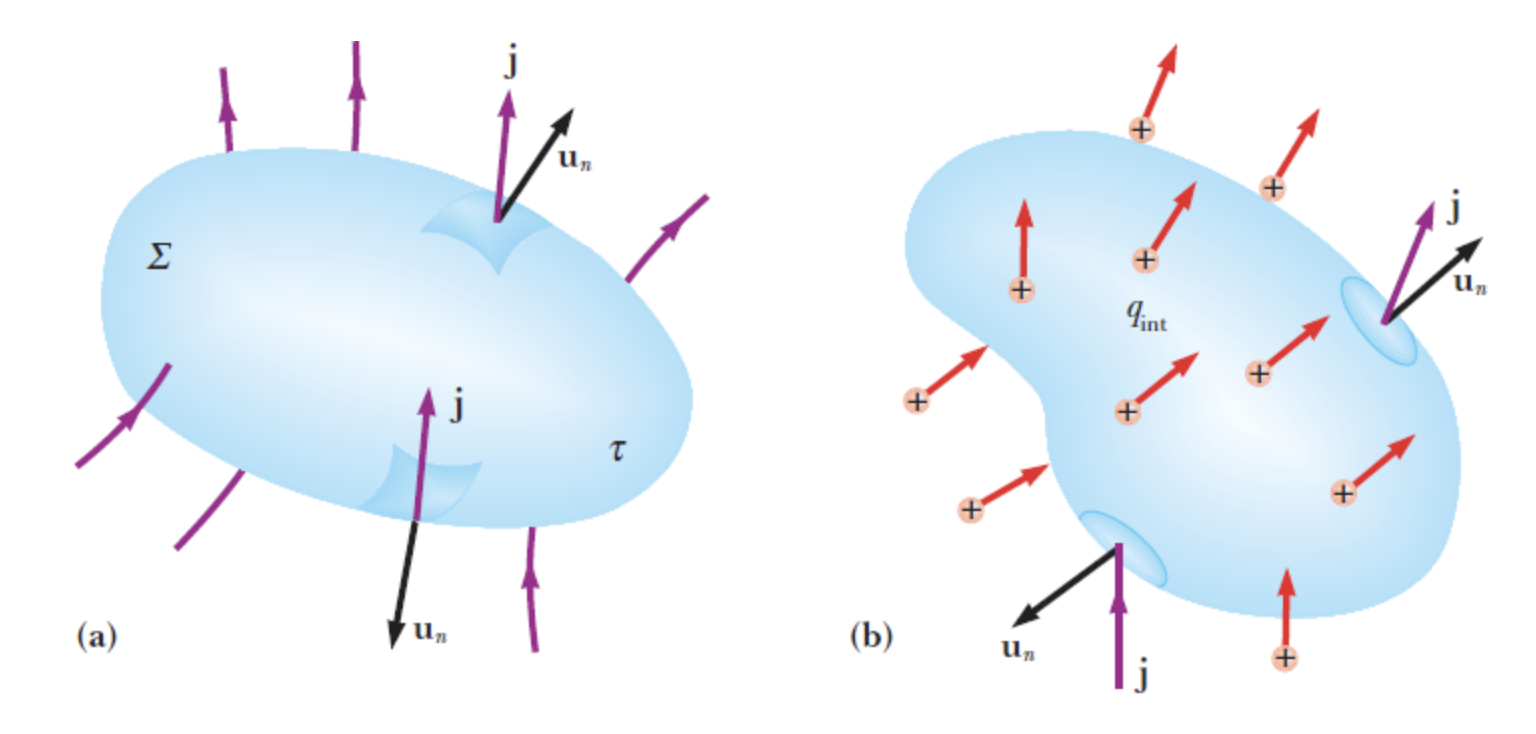
\includegraphics[width=0.75\linewidth]{figure/image39.png}
    \label{fig:chapter_12_1}
\end{figure}

Se la regione è sede di una corrente elettrica, definita dal vettore densità di corrente $\mathbf{J}$, la carica totale che passa nell'unità di tempo attraverso la superficie $\Sigma$ è data dal flusso di $\mathbf{J}$ attraverso $\Sigma$:

\begin{equation}
    I = \oint_{\Sigma} \mathbf{J} \cdot \mathbf{u}_n \ d\Sigma
\end{equation}

Il principio di conservazione della carica richiede che $I$, pari alla carica che attraversa $\Sigma$ nell'unità di tempo, sia eguale alla variazione nell'unità di tempo della carica complessiva $q_{\text{int}}$ contenuta all'interno di $\Sigma$

\begin{tcolorbox}[colback=yellow!10!white, colframe=orange!70!black, boxrule=0.8pt]
\begin{equation}
    I = \oint_{\Sigma} \mathbf{J} \cdot \mathbf{u}_n \ d\Sigma = - \frac{dq_{\text{int}}}{dt}
    \label{eq:principio_conservazione_carica}
\end{equation}
\end{tcolorbox}

\newpage

Un caso particolare e interessante si ha quando la carica interna interna non varia, per cui vale 

\begin{equation}
    \oint_{\Sigma} \mathbf{J} \cdot \mathbf{u}_n \ d\Sigma = 0
\end{equation}

Possiamo ricavare anche una forma locale della \ref{eq:principio_conservazione_carica}. Infatti possiamo scrivere questa può essere scritta come 

\begin{equation}
    \oint_{\Sigma} \mathbf{J} \cdot \mathbf{u}_n \ d\Sigma = - \int_{\tau} \frac{\partial \rho}{\partial t} \ d \tau
\end{equation}

Applicando il teorema della divergenza 

\begin{equation}
    \int_{\tau} \left( \nabla \cdot \mathbf{J} + \frac{\partial \rho}{\partial t} \right) d \tau = 0
\end{equation}

Dato che questo deve valere comunque di scelga il volume $\tau$ si deve avere 

\begin{tcolorbox}[colback=yellow!10!white, colframe=orange!70!black, boxrule=0.8pt]
\begin{equation} \label{eq:equazione_continuità}
    \nabla \cdot \mathbf{J} + \frac{\partial \rho}{\partial t} = 0
\end{equation}
\end{tcolorbox}

Questa \mkeyword{equazione di continuità della corrente} prende il nome di equazione di continuità della corrente ed esprime in modo dinamico la conservazione della carica elettrica.\\

In condizioni stazionarie si ha 

\begin{tcolorbox}[colback=yellow!10!white, colframe=orange!70!black, boxrule=0.8pt]
\begin{equation}
    \nabla \cdot \mathbf{J} = 0
\end{equation}
\end{tcolorbox}

\section{Conduttività elettrica e legge di Ohm}

Nella maggior parte delle sostanze, e in un ampio intervallo di intensità di campo elettrico, scopriamo che la densità di corrente è proporzionale all'intensità del campo elettrico che la causa. La relazione lineare tra densità di corrente e campo è espressa da

\begin{tcolorbox}[colback=yellow!10!white, colframe=orange!70!black, boxrule=0.8pt]
\begin{equation}
    \mathbf{J} = \sigma \ \mathbf{E}
    \label{eq:Legge_Ohm_conduzione}
\end{equation}
\end{tcolorbox}

Il \mkeyword{conduttività} fattore $\sigma$ è chiamato conduttività del materiale. Il suo valore dipende dal materiale in questione; è molto grande per i conduttori metallici, estremamente piccolo per i buoni isolanti. Può dipendere anche dallo stato fisico del materiale, ad esempio dalla sua temperatura.\\

La relazione \ref{eq:Legge_Ohm_conduzione} prende il nome di legge di Ohm della conduzione elettrica. Un'altra sua forma è la seguente

\begin{tcolorbox}[colback=yellow!10!white, colframe=orange!70!black, boxrule=0.8pt]
\begin{equation}
    \mathbf{E} = \rho \ \mathbf{J}
\end{equation}
\end{tcolorbox}

dove $\rho$ prende \mkeyword{resistività}il nome di resistività del conduttore . \footnote{Non andiamo ad approfondire oltre l'argomento, poiché trattato al corso di \emph{Laboratorio 2}}


\chapter{Forza magnatica e Campo magnetico}

I capitoli precedenti sono stati dedicati all'elettrostatica, ovvero allo studio delle interazioni tra cariche \emph{fisse}. Adesso però andremo a trattare dell'interazione delle cariche in moto, studio che è il fondamento della magnetostatica \mkeyword{magnetostatica}. \\

La proprietà di attirare la limatura di ferro, mostrata da alcuni minerali e in particolare dalla magnetite, era già nota nel VII secolo a.C., tuttavia la prima relazione tra fenomeni magnetici ed elettrici fu scoperta da Oersted nel 19° secolo e successivamente l'argomento fu approfondito soprattutto da Ampère. \\

Oersted mostrò che un ago magnetico, posto in prossimità di un filo percorso da corrente, tende ad assumere una ben definita posizione di equilibrio.\\
Se poniamo in un piano perpendicolare al filo percorso da corrente della limatura di ferro osserviamo che questa di addensa lungo circonferenze con centro il filo stesso. \\
Alla luce di quanto visto finora il risultato si interpreta dicendo che il filo percorso da corrente produce un \emph{campo magnetico} \mkeyword{campo magnetico}, che indichiamo con il simbolo $\mathbf{B}$.\\
In seguito Ampère dimostrò che anche due fili percorsi da corrente interagiscono e intuì che \emph{le azioni magnetiche non sono altro che la manifestazione dell'interazione tra cariche elettriche in movimento}.\\

Negli anni successivi Faraday dimostrò che l'esistenza di un'ulteriore connessione tra elettricità e magnetismo, provando che campi magnetici variabili nel tempo producono campi elettrici. Infine Maxwell dimostrò che nel caso più generale un \emph{campo elettrico e un campo magnetico non possono avere esistenza indipendente e vanno unificati nell'unico concetto di campo elettromagnetico}. 


\section{Legge di Gauss per il campo magnetico}

Le osservazioni sperimentali mettono in evidenza che il campo magnetico è una grandezza vettoriale e, in analogia a quanto fatto per il campo elettrostatico, è possibile dare una descrizione del campo magnetico in termini di linee di campo magnetico, \mkeyword{linee di campo magnetico} cioè quelle linee che sono in ogni punto tangenti al campo magnetico $\mathbf{B}$. \\

Per il campo magnetico $\mathbf{B}$, come per il campo elettrostatico $\mathbf{E}$, valgono le seguenti proprietà:

\begin{enumerate}
    \item una linea di campo magnetico è in ogni punto tangente e concorde al campo $\mathbf{B}$ in quel punto
    \item le linee del campo magnetico non si incrociano mai, in quanto in ogni punto il campo $\mathbf{B}$ è definito univocamente 
\end{enumerate}

Come detto sopra le azioni magnetiche non sono altro che la manifestazione dell'interazione tra cariche elettriche in movimento, quindi per descrivere le azioni sui magneti bisogna pensare che in ogni atomo o in ogni molecola devono esistere delle correnti microscopiche locali, che prendono il nome di \mkeyword{correnti amperiane}correnti molecolari di Ampère o correnti amperiane. Ampère provò l'equivalenza tra un circuito percorso da corrente e un dipolo magnetico, sia rispetto alle forze subite ad opera di un campo magnetico, sia per quanto riguarda il campo magnetico prodotto. Avendo allora già sviluppato il formalismo relativo ai dipoli elettrici, è comodo utilizzarlo anche per le azioni magnetiche, senza dargli però un significato fisico profondo.\\

Consideriamo adesso una superficie chiusa $\Sigma$ che racchiuda nel suo interno un magnete permanente o una parte di esso 

\begin{figure} [h]
    \centering
    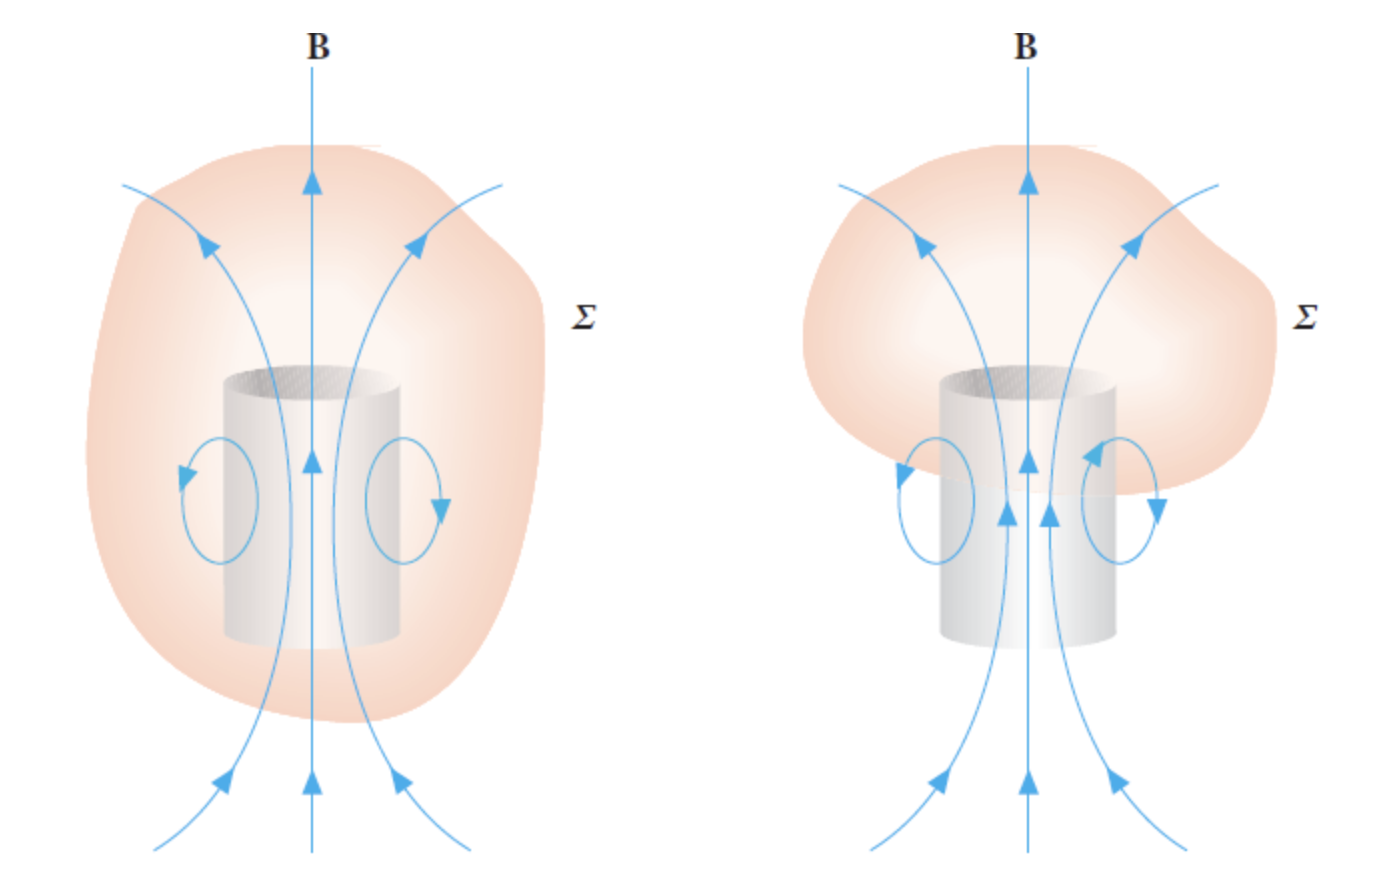
\includegraphics[width=0.75\linewidth]{figure/image40.png}
    \caption{Superficie chiusa che racchiude un magnete permanente}
    \label{fig:chapter_13_1}
\end{figure}


L'equivalenza formale tra le correnti microscopiche e i dipoli magnetici comporta che in entrambi i casi nell'interno della superficie $\Sigma$ sia contenuto un numero intero di dipoli magnetici: una superficie infatti non può mai tagliare uno di questi ipotetici dipoli elementari, operazione che, se i dipoli esistessero realmente, equivarrebbe a isolare due monopòli magnetici Sud e Nord. \\

Da questo punto di vista, la struttura dipolare comporta che la somma delle ipotetiche masse magnetiche sia nulla, per cui per il campo magnetico si può enunciare la legge di Gauss \mkeyword{Legge di Gauss per il campo magnetico}

\begin{tcolorbox}[colback=yellow!10!white, colframe=orange!70!black, boxrule=0.8pt]
\begin{equation}
    \Phi (\mathbf{B}) = \oint_{\Sigma} \mathbf{B} \cdot \mathbf{u}_n \ d \Sigma = 0
\end{equation}
\end{tcolorbox}

Il flusso del campo magnetico attraverso una qualunque superficie chiusa $\Sigma$ è sempre nullo. \\

In termini locali 

\begin{tcolorbox}[colback=yellow!10!white, colframe=orange!70!black, boxrule=0.8pt]
\begin{equation}
    \nabla \cdot \mathbf{B} = 0
\end{equation}
\end{tcolorbox}

Di conseguenza il flusso di $\mathbf{B}$ attraverso le superfici che hanno lo stesso contorno e sono concordemente orientate è sempre lo stesso e si può così parlare in maniera univoca di flusso del campo magnetico attraverso una linea chiusa, ovvero il flusso concatenato con una linea chiusa. \mkeyword{flusso concatenato}

\section{Forza magnetica su una carica in moto}

Consideriamo una particella di massa $m$ e carica $q$, posta in un campo magnetico $\mathbf{B}$. \\

Se la particella è ferma in un sistema di riferimento solidale alle sorgenti del campo magnetico si trova che su di essa non agisce nessuna forza, in accordo con il fatto che l'interazione magnetica si manifesta solamente tra cariche in movimento. \\

Se invece la particella è in moto con velocità $\mathbf{v}$ rispetto al sistema di riferimento suddetto, si verifica che su di essa agisce la \emph{forza di Lorentz} \mkeyword{forza di Lorentz}

\begin{tcolorbox}[colback=yellow!10!white, colframe=orange!70!black, boxrule=0.8pt]
\begin{equation}
    \mathbf{F} = q \mathbf{v} \times \mathbf{B}
\end{equation}
\end{tcolorbox}

Una particolarità di questa forza è il fatto che essa è sempre ortogonale alla velocità, cioè alla traiettoria, e pertanto in base alla definizione di lavoro si ha 

\begin{equation}
    d W = \mathbf{F} \cdot d \mathbf{s} = q \ (\mathbf{v} \times \mathbf{B}) \cdot \mathbf{v} \ dt = 0
\end{equation}

In quanto il vettore $(\mathbf{v} \times \mathbf{B})$ è perpendicolare a $\mathbf{v}$. Pertanto risulta che \emph{la forza di Lorentz non compie lavoro sulla particella}. \\

Questo comporta che l'energia cinetica rimane costante e quindi \emph{quando una particella carica si muove in un campo magnetico la sua velocità cambia in direzione, ma non in modulo}. 

\subsection{Moto in campo magnetico uniforme, $\mathbf{\theta = \pi/2}$}

Supponiamo che il campo magnetico $\mathbf{B}$ sia uniforme in una certa regione e che la velocità iniziale della particella sia ortogonale a $\mathbf{B}$: la forza di Lorentz, anch'essa ortogonale a B, produce una variazione della direzione della velocità ancora ortogonale a B e quindi la velocità in qualsiasi istante successivo sta nel piano ortogonale a B individuato dalla velocità iniziale. \\

\begin{figure}[h]
    \centering
    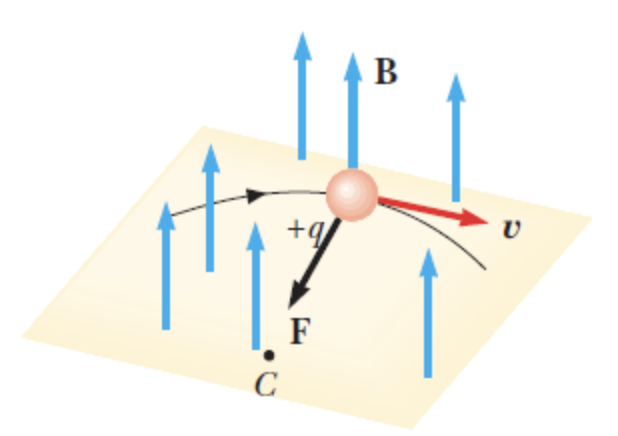
\includegraphics[width=0.37\linewidth]{figure/image41.png}
    \caption{Moto di una carica in un campo magnetico uniforme perpendicolare alla velocità}
    \label{fig:chapter_13_2}
\end{figure}

La legge del moto è

\begin{equation}
    F = q v B = m a_n = m \frac{v^2}{r}
\end{equation}

Pertanto il moto è \emph{circolare uniforme} e il raggio di curvatura $r$ risulta essere

\begin{tcolorbox}[colback=yellow!10!white, colframe=orange!70!black, boxrule=0.8pt]
\begin{equation}
    r = \frac{mv}{qB} = \frac{p}{qB}
\end{equation}
\end{tcolorbox}

Inoltre si ricava facilmente che 

\begin{tcolorbox}[colback=yellow!10!white, colframe=orange!70!black, boxrule=0.8pt]
\begin{equation}
    \omega = \frac{v}{r} = \frac{qB}{m} \quad ; \quad T = \frac{2 \pi}{\omega} = \frac{2 \pi m}{qB}
\end{equation}
\end{tcolorbox}

\subsection{Moto in campo magnetico uniforme, $\theta$ generico}

Se l'angolo $\theta$ che la velocità della particella forma con il campo magnetico è qualsiasi, scomponiamo la velocità $\mathbf{v}$ nelle due componenti $v_n = v \sin \theta$ ortogonale a $\mathbf{B}$ e $v_p = v \cos \theta $ parallela a $\mathbf{B}$. 

\begin{figure} [h]
    \centering
    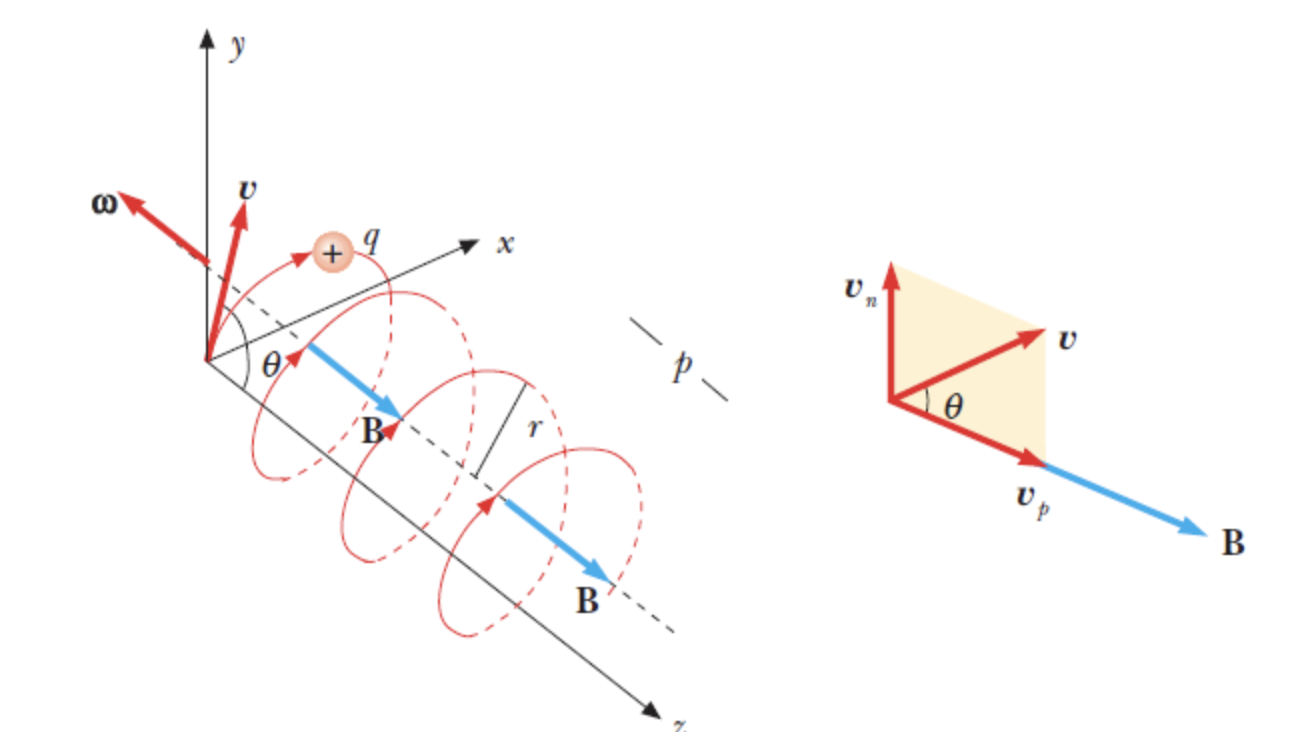
\includegraphics[width=0.7\linewidth]{figure/image42.png}
    \caption{Moto elicoidale di una particella con carica positiva in campo magnetico uniforme}
    \label{fig:chapter_13_3}
\end{figure}

La forza magnetica che agisce sulla particella è

\begin{equation}
    \mathbf{F} = q \mathbf{v}_n \times \mathbf{B} 
\end{equation}

Abbiamo pertanto in un piano ortogonale a $\mathbf{B}$ un moto circolare uniforme con velocità $v_n$, eguale a quello descritto nel caso precedente; svolgendo gli stessi ragionamenti precedenti, si ottiene

\begin{tcolorbox}[colback=yellow!10!white, colframe=orange!70!black, boxrule=0.8pt]
\begin{equation}
    r = \frac{mv \sin \theta}{q B}
\end{equation}
\end{tcolorbox}

\newpage

\section{Forza magnetica su un conduttore percorso da corrente}

La corrente elettrica in un conduttore è dovuta al moto degli elettroni sotto l'azione del campo elettrico applicato tramite un generatore, pertanto quando il conduttore percorso da corrente è immerso in un campo magnetico a ciascun elettrone è applicata la forza di Lorentz:

\begin{equation*}
    \mathbf{F}_L = - e \mathbf{v}_d \times \mathbf{B}
\end{equation*}

Quindi in un tratto lungo $d s$ e si sezione $\Sigma$ sono contenuti $n \Sigma \ ds$ elettroni e la forza risultante è 

\begin{equation*}
    d \mathbf{F} = n \Sigma \ ds \ \mathbf{F}_L = - (\Sigma ds) n e \mathbf{v}_d \times \mathbf{B} = \Sigma ds \ \mathbf{j} \times \mathbf{B}
\end{equation*}

Essendo $\Sigma ds$ eguale al volume infinitesimo $d\tau$, si vede che la forza agente per unità di volume sul conduttore è

\begin{tcolorbox}[colback=yellow!10!white, colframe=orange!70!black, boxrule=0.8pt]
\begin{equation}
    \mathbf{F}_{\tau} = \mathbf{j} \times \mathbf{B}
\end{equation}
\end{tcolorbox}

D'altra parte, \emph{riferendoci a un conduttore filiforme} e ricordando che $\Sigma j$ è la corrente $i$ che percorre il filo, oritentiamo $d \mathbf{s}$ come $\mathbf{j}$ e otteniamo 

\begin{tcolorbox}[colback=yellow!10!white, colframe=orange!70!black, boxrule=0.8pt]
\begin{equation} \label{eq:seconda_legge_elementare_Laplace}
    d \mathbf{F} = i \ d \mathbf{s} \times \mathbf{B}
\end{equation}
\end{tcolorbox}

Questa relazione è nota come seconda legge elementare di Laplace. \mkeyword{seconda legge fondamentale di Laplace}\\

Allora per ottenere la forza su un tratto di filo indeformabile di lunghezza infinita, percorsa da corrente (stazionaria) $i$, si integra la \ref{eq:seconda_legge_elementare_Laplace}:

\begin{tcolorbox}[colback=yellow!10!white, colframe=orange!70!black, boxrule=0.8pt]
\begin{equation} \label{eq:seconda_legge_elementare_Laplace_integrata}
    \mathbf{F} = i \int_{P}^{Q}\ d \mathbf{s} \times \mathbf{B}
\end{equation}
\end{tcolorbox}

Dove $P$ e $Q$ sono gli estremi del filo. \\

\subsection{Campo magnetico uniforme e filo rettilineo}

Supponiamo che il campo magnetico sia uniforme e che il conduttore sia rettilineo, di lunghezza l. Allora la \ref{eq:seconda_legge_elementare_Laplace_integrata} si semplifica in

\begin{equation*}
    \mathbf{F} = i \left( \int_{P}^{Q} d \mathbf{s} \right) \times \mathbf{B}
\end{equation*}

in quanto sia il modulo del campo che l'angolo $\theta$ formato con $d \mathbf{s}$ sono costanti durante l'integrazione, e si ha 

\begin{tcolorbox}[colback=yellow!10!white, colframe=orange!70!black, boxrule=0.8pt]
\begin{equation} 
     \mathbf{F} = i \mathbf{l} \times \mathbf{B}
\end{equation}
\end{tcolorbox}

\subsection{ Campo magnetico uniforme e filo curvilineo piano}

Supponiamo ora che il campo magnetico sia uniforme, ma che il filo non sia rettilineo: esso può essere anche curvilineo, purché giaccia interamente in un piano (ad esempio il piano $xy$). \\

\'E facile verificare che 

\begin{tcolorbox}[colback=yellow!10!white, colframe=orange!70!black, boxrule=0.8pt]
\begin{equation} 
     \mathbf{F} = i \mathbf{PQ} \times \mathbf{B}
\end{equation}
\end{tcolorbox}

Pertanto la forza su un filo percorso da corrente che giace in un piano in cui agisce un campo magnetico uniforme $\mathbf{B}$ non dipende dalla forma del filo, ma solo dalla lunghezza del segmento che unisce i suoi estremi. \\

Inoltre \emph{la forza su un circuito che sta su un piano in cui agisce un campo magnetico $\mathbf{B}$ uniforme è nulla.}



\chapter{Sorgenti del campo magnetico}

Nel capitolo precedente abbiamo trattato come un campo magnetico agisce su una carica, o un sistema di cariche, in movimento, tuttavia non abbiamo ancora parlato del legame esplicito tra il campo magnetico e le correnti che lo generano. \\

Di seguito andremo a trovare delle espressioni analoghe a quelle gia viste per il campo elettrico, relative, pero, al legame del campo magnetico con le cariche in moto. 

\section{Campo magnetico prodotto da una corrente}

L'analisi dei primi esperimenti sulle caratteristiche del campo magnetico prodotto da correnti in conduttori filiformi indusse Laplace a formulare una legge, nota come \emph{prima legge elementare di Laplace}, \mkeyword{prima legge elementare di Laplace} che esprime il campo magnetico prodotto da un tratto infinitesimo $ds$ di filo, percorso dalla corrente $i$, in un punto $P$ distante $r$ dall'elemento di filo

\begin{tcolorbox}[colback=yellow!10!white, colframe=orange!70!black, boxrule=0.8pt]
\begin{equation} \label{eq:legge_el_Laplace}
    d \mathbf{B} = \frac{\mu_0 i}{4 \pi} \frac{d \mathbf{s} \times \mathbf{u}_r}{r^2} = \frac{\mu_0 }{4 \pi} \frac{i \ d s}{r^2} \mathbf{u}_t \times \mathbf{u}_r 
\end{equation}
\end{tcolorbox}

Dove $\mathbf{u}_r$ è il versore della direzione orientata da $d s$ a $P$, $\mathbf{u}_t$ il versore tangente al filo per cui $d \mathbf{s} = ds \ \mathbf{u}_t$. 

\begin{figure}[h]
    \centering
    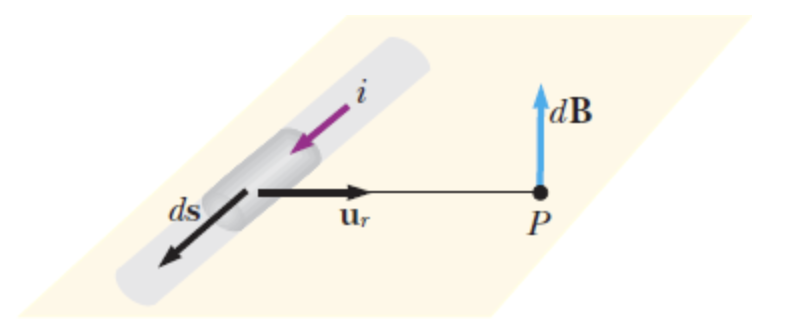
\includegraphics[width=0.7\linewidth]{figure/image43.png}
    \caption{Campo magnetico prodotto da un elemento di filo percorso da corrente}
    \label{fig:campo_magnetico_filo}
\end{figure}

Mentre $\mu_0$ è una costante che prende il nome di \emph{permeabilità nel vuoto} \mkeyword{permeabilità nel vuoto} e risulta

\begin{tcolorbox}[colback=yellow!10!white, colframe=orange!70!black, boxrule=0.8pt]
\begin{equation}
    \mu_0 = 1,26 \cdot 10^{-6} \ \frac{H}{m}
\end{equation}
\end{tcolorbox}

La \ref{eq:legge_el_Laplace} ha validità generale soltanto come strumento matematica di calcolo: sperimentalmente non è possibile misurare il contributo di un elemento infinitesimo del filo, che non può esistere da solo. \\

Ciò che ha significato fisico, e si può misurare, è la sovrapposizione dei contribui, cioè l'integrale di \ref{eq:legge_el_Laplace} esteso a un circuito chiuso $C$

\begin{tcolorbox}[colback=yellow!10!white, colframe=orange!70!black, boxrule=0.8pt]
\begin{equation}\label{eq:legge_Ampere-Laplace}
    \mathbf{B} = \frac{\mu_0 i}{4 \pi} \oint_C \frac{d\mathbf{s} \times \mathbf{u}_r}{r^2}
\end{equation}
\end{tcolorbox}

Questo risultato costituisce la \emph{legge di Ampère-Laplace}. \mkeyword{legge di Ampère-Laplace}\\

La \ref{eq:legge_Ampere-Laplace} dà in ogni punto dello spazio il campo magnetico dovuto a un circuito chiuso \emph{filiforme} fi forma qualunque. \\

Più in generale se il conduttore non è filiforme si considera un elemento lungo $d s$, di sezione $d \Sigma$, percorso da una corrente di intensità $\mathbf{j}$, quindi vale

\begin{equation*}
    d i \ d\mathbf{s} = \mathbf{j} \ d\Sigma \ ds = \mathbf{j} \  d \tau
\end{equation*}

Sostituendo nella \ref{eq:legge_el_Laplace} si ottiene 

\begin{tcolorbox}[colback=yellow!10!white, colframe=orange!70!black, boxrule=0.8pt]
\begin{equation}
    d\mathbf{B} = \frac{\mu_0 }{4 \pi} \frac{\mathbf{j} \times \mathbf{u}_r}{r^2} d\tau
\end{equation}
\end{tcolorbox}

e integrando in tutto il volume in cui $\mathbf{j}$ è diverso da zero si ottiene 

\begin{tcolorbox}[colback=yellow!10!white, colframe=orange!70!black, boxrule=0.8pt]
\begin{equation}\label{eq:legge_Ampere-Laplace_generale}
    \mathbf{B} = \frac{\mu_0 }{4 \pi} \int_{\tau} \frac{\mathbf{j} \times \mathbf{u}_r}{r^2} d\tau
\end{equation}
\end{tcolorbox}

Nel capitolo precedente abbiamo dedotto che il campo magnetico è solinoidale, adesso lo possiamo mostrare esplicitamente

\subsection{Divergenza del campo magnetico}

Riscriviamo la \ref{eq:legge_Ampere-Laplace_generale} nella forma 

\begin{equation*}
    \mathbf{B}(x,y,z) = \frac{\mu_0 }{4 \pi} \int_{\tau} \frac{\mathbf{j}(x',y',z') \times \mathbf{u}_r}{r^2} d\tau
\end{equation*}

Dove indichiamo con gli elementi non primati quelli che si riferiscono alla posizione del punto in cui andiamo a cercare il campo, mentre con gli elementi primati quelli che riferiscono ai punti del volume $\tau$. La divergenza di $\mathbf{B}$ è 

\begin{equation*}
    \nabla \cdot \mathbf{B} = \frac{\mu_0 }{4 \pi} \nabla \cdot \int_{\tau} \frac{\mathbf{j}(x',y',z') \times \mathbf{u}_r}{r^2} d\tau
\end{equation*}

Dato che la divergenza è calcolata rispetto alle coordinate $(x,y,z)$ mentre l'integrazione è fatta sulle coordinate $(x',y',z')$, per cui possiamo scrivere 

\begin{equation*}
    \nabla \cdot \mathbf{B} = \frac{\mu_0 }{4 \pi} \int_{\tau} \nabla \cdot \left[ \frac{\mathbf{j}(x',y',z') \times \mathbf{u}_r}{r^2} \right] d\tau = - \frac{\mu_0 }{4 \pi} \int_{\tau} \nabla \cdot \left[ \mathbf{j}(x',y',z') \times \nabla \left( \frac{1}{r} \right) \right] d\tau
\end{equation*}

Dove abbiamo posto $\mathbf{u}_r/r^2 = - \nabla(1/r)$. \\

Sfruttando l'identità $\nabla \cdot (\mathbf{a}\times \mathbf{b}) = \mathbf{b} \cdot \nabla \times \mathbf{a} - \mathbf{a} \times \nabla \times \mathbf{b}$ si ha:

\begin{align*}
    \nabla \cdot \left[ \mathbf{j}(x',y',z') \times \nabla \left( \frac{1}{r} \right) \right] = \\
    = \nabla \left( \frac{1}{r} \right) \cdot \nabla \times \mathbf{j} (x',y',z') - \mathbf{j}(x',y',z') \cdot \nabla \times \nabla \left( \frac{1}{r} \right) = 0
\end{align*}

dato che $\nabla$ opera sulle coordinate $(x,y,z)$, mentre $\mathbf{j}$ dipende da $(x',y',z')$, e che il rotore di un gradiente è identicamente nullo. \\

Applichiamo adesso la prima legge elementare di Laplace ad alcune configurazioni in cui la corrente percorre un conduttore filiforme di forma semplice.

\subsection{Filo rettilineo indefinito. Legge di Biot-Savart}

Consideriamo un filo conduttore rettilineo, di lunghezza $2a$, percorso dalla corrente $i$, e poniamoci nel piano mediano del filo nel punto $P$ distante $R$ dal filo. 

\begin{figure}[h]
    \centering
    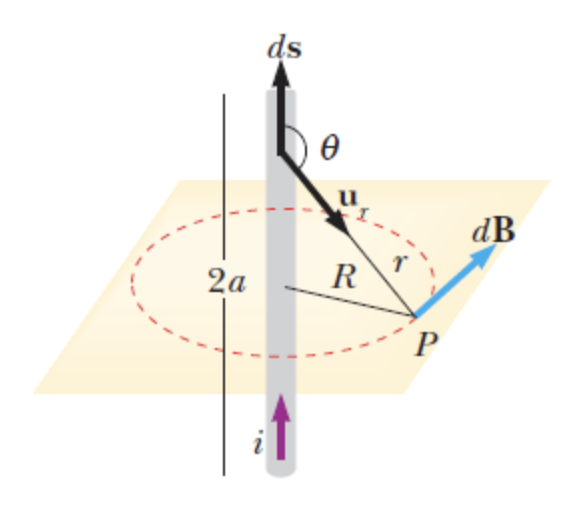
\includegraphics[width=0.5\linewidth]{figure/image44.png}
    \caption{Filo rettilineo}
    \label{fig:chapter_14_1}
\end{figure}

Un elemento di filo produce in $P$ il campo magnetico 

\begin{equation*}
    d \mathbf{B} = \frac{\mu_0 i}{4 \pi} \frac{d \mathbf{s} \times \mathbf{u}_r}{r^2} \implies dB = \frac{\mu_0 i}{4 \pi} \frac{ds \sin\theta}{r^2}
\end{equation*}

\'E conveniente andare ad esprimere $r$ e $ds$ in funzione di $\theta$. 

\begin{align*}
    r \sin (\pi - \theta) = r \sin\theta = R \implies \frac{1}{r^2} = \frac{\sin^2 \theta}{r^2},\\
    \text{tg}(\pi - \theta) = - \text{tg}\theta = \frac{R}{s} \implies ds = \frac{R d \theta}{\sin^2 \theta} , 
\end{align*}

\newpage

Quindi, sostituendo, si ottiene 

\begin{equation}
    dB = \frac{\mu_0 i}{4 \pi} \frac{\sin \theta \ d \theta}{R} =-\frac{\mu_0 i}{4 \pi} \frac{ d(\cos \theta) }{R}
\end{equation}

Possiamo trovare il campo generato da tutto il filo integrando 

\begin{equation*}
    B = -\frac{\mu_0 i}{4 \pi R} \int_{-\cos(\bar{\theta})}^{\cos(\bar{\theta})} d(\cos \theta) = \frac{\mu_0 i \cos(\bar{\theta})}{2 \pi R}
\end{equation*}

Allora, andando a sostituire $\cos(\bar{\theta})$ e sfruttando la simmetria per rotazione intorno all'asse passante per il filo si ottiene 

\begin{tcolorbox}[colback=yellow!10!white, colframe=orange!70!black, boxrule=0.8pt]
\begin{equation}
    \mathbf{B} = \frac{\mu_0 i a }{2 \pi R \sqrt{R^2 + a^2}} \mathbf{u}_{\phi}
\end{equation}
\end{tcolorbox}

In particolare se facciamo tendere la lunghezza $a$ all'infinito questa diventa 

\begin{tcolorbox}[colback=yellow!10!white, colframe=orange!70!black, boxrule=0.8pt]
\begin{equation} \label{eq:legge_Biot-Savart}
    \mathbf{B} = \frac{\mu_0 i }{2 \pi R } \mathbf{u}_{\phi}
\end{equation}
\end{tcolorbox}

Quest ultima è nota come \emph{legge di Biot-Savart} \mkeyword{legge di Biot-Savart} e afferma che il campo magnetico di un filo rettilineo indefinito dipende solo dalla distanza del filo, in modo inversamente proporzionale. 

\subsection{Spira circolare}

Passiamo ora a calcolare il campo magnetico sull'asse di una spira circolare di raggio $R$, percorsa da corrente $i$. 

\begin{figure} [h]
    \centering
    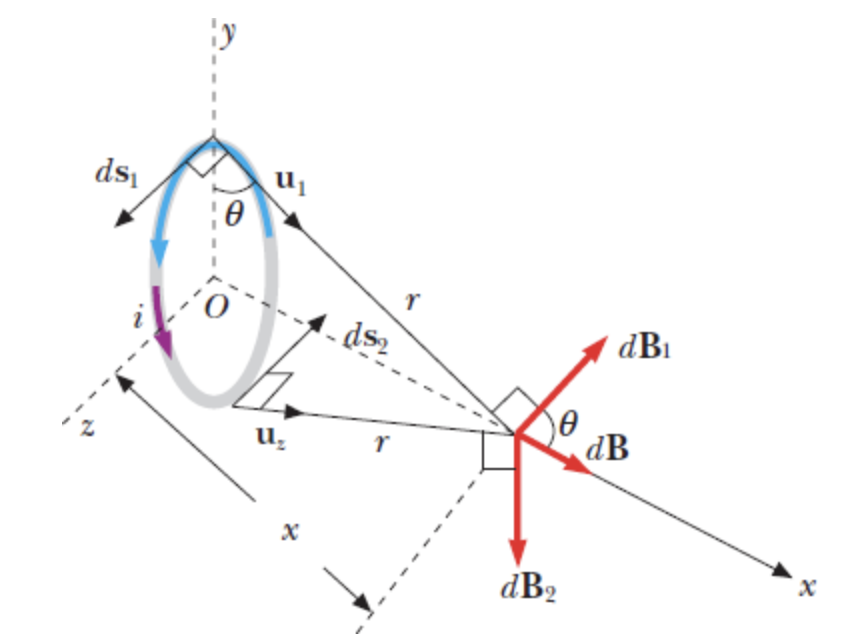
\includegraphics[width=0.6\linewidth]{figure/image45.png}
    \caption{Campo magnetico sull'asse di una sprira circolare}
    \label{fig:chapter_14_2}
\end{figure}

Nel punto $P$, distante $x$ da centro $O$ della spira, un elemento $d \mathbf{s}$ di spira genera il campo $d \mathbf{B}$ di modulo 

\begin{equation*}
    dB = \frac{\mu_0 i \ ds}{4 \pi r^2}
\end{equation*}

in quanto $d \mathbf{s}$ e $\mathbf{u}_r$ sono ortogonali. \\

La componente lungo l'asse $x$ vale 

\begin{equation*}
    dB_x = \frac{\mu_0 i \ ds}{4 \pi r^2} \cos \theta
\end{equation*}

dove $\theta$ è l'angolo che $d \mathbf{B}$ forma con l'asse $x$. Quando si considerano i contributi $d \mathbf{B}$ di tutti gli elementi $d \mathbf{s}$ che formano la spira, le componenti parallele all'asse si sommano, mentre quelle trasversali si elidono a due a due, per la simmetria del problema.

\begin{equation*}
    \mathbf{B} = \oint \frac{\mu_0 i}{4 \pi} \frac{\cos \theta}{r^2} ds \ \mathbf{u}_n = \frac{\mu_0 i}{4 \pi} \frac{\cos \theta}{r^2} 2 \pi R \ \mathbf{u}_n
\end{equation*}

Posto $r^2 = x^2 + R^2$ e $\cos \theta = R/r$ si ottiene 

\begin{tcolorbox}[colback=yellow!10!white, colframe=orange!70!black, boxrule=0.8pt]
\begin{equation} \label{eq:campo_spira_circolare}
    \mathbf{B} = \frac{\mu_0 i R^2}{2 r^3} \mathbf{u}_n = \frac{\mu_0 i R^2}{2 (x^2 + R^2)^{3/2}} \mathbf{u}_n
\end{equation}
\end{tcolorbox}

Allora nel centro della spira il campo è massimo e vale 

\begin{tcolorbox}[colback=yellow!10!white, colframe=orange!70!black, boxrule=0.8pt]
\begin{equation} 
    \mathbf{B} = \frac{\mu_0 i }{2 R} \mathbf{u}_n
\end{equation}
\end{tcolorbox}

Mentre per $x \to \infty$ il campo tende a zero.

\subsection{Solenoide rettilineo}

Un solenoide rettilineo è costituito da un filo conduttore avvolto a forma di elica cilindrica di piccolo passo. Sia $d$ la lunghezza del solenoide, $R$ il raggio, $N$ il numero totale di spire, $n = N/d$ il numero di spire per unità di lunghezza.

\begin{figure} [h]
    \centering
    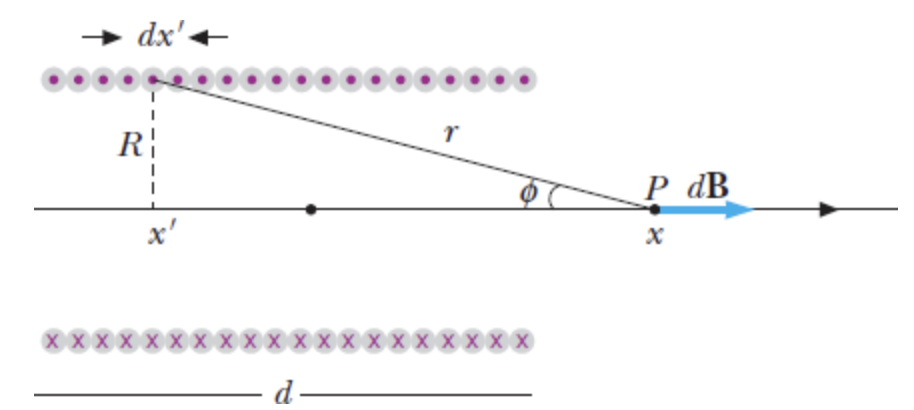
\includegraphics[width=0.6\linewidth]{figure/image46.png}
    \caption{Campo magnetico sull'asse di un solenoide rettilineo}
    \label{fig:chapter_14_3}
\end{figure}

Se le spire sono abbastanza fitte, così da poterle considerare distribuite con continuità, nel tratto di lunghezza $dx'$, di coordinata $x'$ rispetto ad un'origine $O$ sull'asse del solenoide, ce ne sono $ndx$. Il valore del campo magnetico in un punto $P$ sull'asse, di coordinata $x$, si calcola sfruttando la \ref{eq:campo_spira_circolare}, infatti il campo magnetico infinitesimo dato dalle spire nell'interavallo $dx'$ che si trovano nel punto $x'$ è data da 

\begin{equation*}
    dB = \frac{\mu_0 i R^2 n }{2r^3} dx'
\end{equation*}

\newpage

Per il calcolo del campo magnetico totale è conveniente introdurre la variabile $\phi$ e andare a esprimere $r$ e $dx'$ in funzione di questa: 

\begin{equation*}
    r = \frac{R}{\sin \phi} \quad , \quad \frac{R}{x - x'} = \text{tg}\phi \implies dx' = \frac{R d\phi }{\sin^2 \phi}
\end{equation*}

Sostituendo e integrando 

\begin{equation*}
    B = \frac{\mu_0 n i}{2} \int_{\phi_1}^{\phi_2} \sin \phi \ d \phi = \frac{\mu_0 n i}{2} (\cos \phi_1 - \cos \phi_2)
\end{equation*}

Esprimendo tutto in funzione della distanza $x$ dal centro del solenoide si ottiene

\begin{tcolorbox}[colback=yellow!10!white, colframe=orange!70!black, boxrule=0.8pt]
\begin{equation} 
    \mathbf{B} = \frac{\mu_0 n i}{2} \left[ \frac{d +2x}{\sqrt{(d+2x)^2 + 4R^2}} + \frac{d-2x}{\sqrt{(d-2x^2) + 4R^2}}  \right] \mathbf{u}_n
\end{equation}
\end{tcolorbox}

Si nota, allora, che il campo magnetico è massimo al centro della spira 

\begin{tcolorbox}[colback=yellow!10!white, colframe=orange!70!black, boxrule=0.8pt]
\begin{equation} 
    \mathbf{B}(O)= \mu_0 \ n i \frac{d}{\sqrt{d^2 + 4R^2}}  \mathbf{u}_n
\end{equation}
\end{tcolorbox}

Mentre nel centro di una spira estrema, cioè quando $x = \pm d/2$, si ha 

\begin{tcolorbox}[colback=yellow!10!white, colframe=orange!70!black, boxrule=0.8pt]
\begin{equation} 
    \mathbf{B}\left(\pm \frac{d}{2}\right)= \frac{\mu_0 \ n i}{2} \frac{d}{\sqrt{d^2 + R^2}}  \mathbf{u}_n
\end{equation}
\end{tcolorbox}

In particolare, se la lunghezza del solenoide è molto maggiore del raggio, il campo magetico in $O$ vale 

\begin{tcolorbox}[colback=yellow!10!white, colframe=orange!70!black, boxrule=0.8pt]
\begin{equation} 
    \mathbf{B}_{\infty}= \mu_0 \ n i \ \mathbf{u}_n
\end{equation}
\end{tcolorbox}

\newpage

\section{Azioni elettrodinamiche tra circuiti percorsi da corrente}

Calcoliamo la forza tra due circuiti percorsi da corrente. \\

\begin{figure}[h]
    \centering
    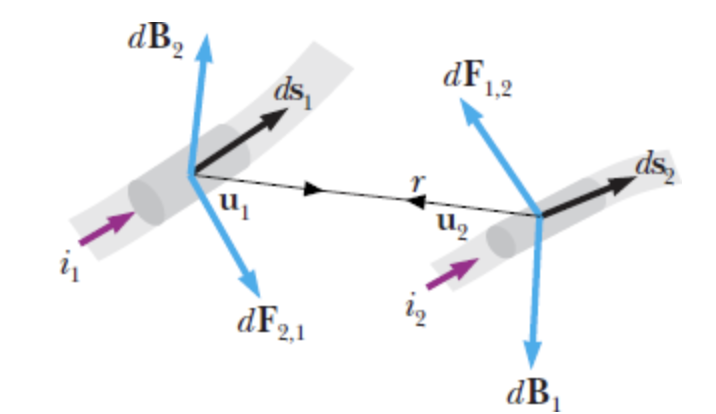
\includegraphics[width=0.6\linewidth]{figure/image47.png}
    \caption{Forza tra due tratti di circuito}
    \label{fig:chapter_14_4}
\end{figure}

Detti $d \mathbf{s}_1$ e $d \mathbf{s}_2$ gli elementi di filo dei circuiti e $i_1$ e $i_2$ le rispettive correnti. La forza $d \mathbf{F}_{1,2}$ agente sull'elemento $d\mathbf{s}_2$ a causa del campo magnetico $d \mathbf{B}_1$ prodotto da $d\mathbf{s}_1$ risulta

\begin{equation}
    d \mathbf{F}_{1,2} = i_2 \ d \mathbf{s}_2 \times d \mathbf{B}_1 = \frac{\mu_0 i_1 i_2}{4 \pi} \frac{ d \mathbf{s}_2 \times (d \mathbf{s}_1 \times \mathbf{u}_1)}{r^2}
\end{equation}

Mentre la forza esercitata da $d \mathbf{s}_2$ su $d \mathbf{s}_1$ è data da 

\begin{equation}
    d \mathbf{F}_{2,1} = \frac{\mu_0 i_1 i_2}{4 \pi} \frac{ d \mathbf{s}_1 \times (d \mathbf{s}_2 \times \mathbf{u}_2)}{r^2}
\end{equation}

Non è difficile trovare situazioni particolari in cui $d\mathbf{F}_{1,2} \neq - d\mathbf{F}_{2,1}$, in contrasto con il principio di azione e reazione; il fatto tuttavia non è preoccupante in quanto, come è stato notato, le leggi elementari di Laplace, considerate a sé, non si applicano a sistemi fisicamente realizzabili.\\

La forza risultante tra i due circuiti si ottiene con una doppia integrazione estesa ai due circuiti che tiene conto di tutte le coppie di elementi $d\mathbf{s}_1$ e $d \mathbf{s}_2$ tra i quali si esercitano le forze $d \mathbf{F}$:

\begin{tcolorbox}[colback=yellow!10!white, colframe=orange!70!black, boxrule=0.8pt]
\begin{equation} 
    \mathbf{F}_{1,2} = \frac{\mu_0 i_1 i_2}{4 \pi} \oint_1 \oint_2 \frac{d \mathbf{s}_2 \times (d\mathbf{s}_1 \times \mathbf{u}_1)}{r^2} \quad , \quad \mathbf{F}_{2,1} = \frac{\mu_0 i_1 i_2}{4 \pi} \oint_2 \oint_1 \frac{d \mathbf{s}_1 \times (d\mathbf{s}_2 \times \mathbf{u}_2)}{r^2}
\end{equation}
\end{tcolorbox}

\'E possibile dimostrare che 

\begin{equation}
    \mathbf{F}_{12} + \mathbf{F}_{21} = 0
\end{equation}

Quindi vale il principio di azione e reazione. 

\subsection{Forza tra due fili rettilinei}

Esaminiamo il caso di due fili rettilinei, percorsi rispettivamente dalle correnti $i_1$ e $i_2$, molto lunghi e abbastanza vicini da poter essere considerati indefiniti. \\

Se essi sono perpendicolari l'uno all'altro la forza tra i due fili è nulla: infatti ciascun filo risulta parallelo al campo magnetico prodotto dall'altro. \\

Consideriamo il caso in cui i due fili sono paralleli 

\begin{figure} [h]
    \centering
    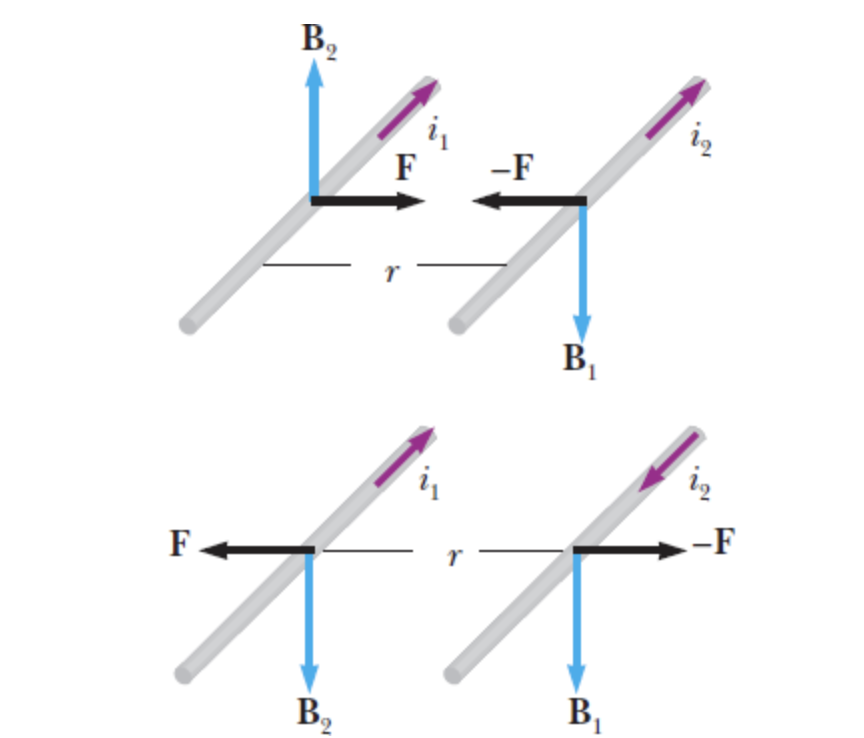
\includegraphics[width=0.5\linewidth]{figure/image48.png}
    \caption{Forza tra due fili indefiniti paralleli percorsi da corrente}
    \label{fig:chapter_14_5}
\end{figure}

Se i due fili, rispettivamente di lunghezza $l_1$ e $l_2$ e distanti $r$ sono paralleli, ciascun filo è perpendicolare al campo magnetico prodotto dall'altro, pertanto vale

\begin{equation}
    \mathbf{F}_{1,2} = i_2 \mathbf{l}_2 \times \mathbf{B}_1 \quad , \quad \mathbf{F}_{2,1} = i_1 \mathbf{l_1} \times \mathbf{B}_2 
\end{equation}

Le due forze, entrambe diretta secondo la congiungente dei fili, sono attrattive se le due correnti sono equiverse e repulsive se sono contrarie.\\
Il modulo della forza per unità di lunghezza di filo è data da 

\begin{tcolorbox}[colback=yellow!10!white, colframe=orange!70!black, boxrule=0.8pt]
\begin{equation}
    F_l = \frac{F_{1,2}}{l_2} = \frac{F_{2,1}}{l_1} = \mu_0 \frac{i_1 i_2}{2 \pi r}
\end{equation}
\end{tcolorbox}

avendo utilizzato la \ref{eq:legge_Biot-Savart} per il campo magnetico. 

\newpage 

\section{Legge di Ampère}

Sappiamo che nel caso generale vale la \ref{eq:legge_Ampere-Laplace_generale}, che, ponendo $r = |\mathbf{r} - \mathbf{r'}|$ dove $\mathbf{r}$ rappresenta la posizione dove stiamo calcolando il campo magnetico, mentre $\mathbf{r'}$ è la posizione di un particolare punto della sorgente del campo, diventa 

\begin{equation}
    \mathbf{B}(\mathbf{r}) = \frac{\mu_0}{4 \pi} \int_{\tau} \mathbf{j} (\mathbf{r'}) \times \frac{\mathbf{r} - \mathbf{r'}}{|\mathbf{r} - \mathbf{r'}|^3} d\tau
\end{equation}

In modo analogo a quanto fatto per il calcolo della divergenza del campo, si ha 

\begin{equation*}
    \mathbf{B}(\mathbf{r}) = - \frac{\mu_0}{4 \pi} \int_{\tau} \mathbf{j} (\mathbf{r}') \times \nabla\left( \frac{1}{|\mathbf{r} - \mathbf{r'}|} \right) d\tau
\end{equation*}

Utilizzando ora l'anticommutatività del prodotto vettoriale,

\begin{equation*}
    \mathbf a \times \mathbf b = - \mathbf b \times \mathbf a
\end{equation*}

segue che

\begin{equation*}
    \mathbf{B}(\mathbf{r})
    = \frac{\mu_0}{4 \pi} \int_{\tau}
    \nabla \left( \frac{1}{|\mathbf r - \mathbf r'|} \right)
    \times \mathbf{j}(\mathbf r') \, d\tau.
\end{equation*}

A questo punto si utilizza l'identità vettoriale

\begin{equation}
    \nabla \times (f \mathbf A)
    = (\nabla f) \times \mathbf A + f (\nabla \times \mathbf A).
\end{equation}

Ponendo

\begin{equation*}
f(\mathbf r)=\frac{1}{|\mathbf r - \mathbf r'|}, \qquad \mathbf A=\mathbf j(\mathbf r'),
\end{equation*}

e osservando che $\mathbf j(\mathbf r')$ dipende solo dalle coordinate primate e quindi risulta costante rispetto all'operatore $\nabla_{\mathbf r}$, si ha

\begin{equation*}
    \nabla \times \mathbf j(\mathbf r') = 0.
\end{equation*}

Segue dunque

\begin{equation*}
    \nabla \times \left( \frac{\mathbf j(\mathbf r')}{|\mathbf r - \mathbf r'|} \right)
    =
    \nabla \left( \frac{1}{|\mathbf r - \mathbf r'|} \right)
    \times \mathbf j(\mathbf r').
\end{equation*}

L'espressione del campo magnetico diventa quindi

\begin{equation*}
    \mathbf{B}(\mathbf{r})
    =
    \frac{\mu_0}{4 \pi}
    \int_{\tau}
    \nabla \times
    \left(
    \frac{\mathbf j(\mathbf r')}{|\mathbf r - \mathbf r'|}
    \right) d\tau.
\end{equation*}

Poiché l'operatore rotore agisce sulle variabili $\mathbf r$ mentre l'integrazione è estesa alle variabili primate $\mathbf r'$, esso può essere portato fuori dal segno di integrale:

\begin{equation} \label{eq:forma_util_legge_Ampère-Laplace}
    \mathbf{B}(\mathbf{r})
    =
    \frac{\mu_0}{4 \pi}
    \nabla \times
    \int_{\tau}
    \frac{\mathbf j(\mathbf r')}{|\mathbf r - \mathbf r'|} \, d\tau.
\end{equation}

Dopo queste prime operazioni iniziali, possiamo adesso passare al calcolo effettivo del rotore di $\mathbf{B}(\mathbf{r})$. \\

A partire dalla \ref{eq:forma_util_legge_Ampère-Laplace} si ha dunque

\begin{equation*}
    \nabla \times \mathbf B(\mathbf r)
    =
    \frac{\mu_0}{4\pi}\,
    \nabla \times \nabla \times
    \int_{\tau}\frac{\mathbf j(\mathbf r')}{|\mathbf r-\mathbf r'|}\,d\tau'
\end{equation*}

Per semplificare la notazione, introduciamo il campo ausiliario

\begin{equation*}
    \mathbf A(\mathbf r)\equiv \int_{\tau}\frac{\mathbf j(\mathbf r')}{|\mathbf r-\mathbf r'|}\,d\tau',
\end{equation*}

cosicché

\begin{equation}\label{eq:curlcurlA}
    \nabla \times \mathbf B(\mathbf r)
    =
    \frac{\mu_0}{4\pi}\,\nabla \times (\nabla \times \mathbf A)
\end{equation}

Usando l'identità vettoriale (valida per un campo vettoriale arbitrario $\mathbf A$)

\begin{equation}
    \nabla \times (\nabla \times \mathbf A)=\nabla(\nabla\cdot \mathbf A)-\nabla^2\mathbf A,
\end{equation}

la \ref{eq:curlcurlA} diventa

\begin{equation}\label{eq:step1}
    \nabla \times \mathbf B(\mathbf r)
    =
    \frac{\mu_0}{4\pi}\left[
    \nabla(\nabla\cdot \mathbf A)-\nabla^2\mathbf A
    \right].
\end{equation}

Poiché l'operatore $\nabla$ agisce sulle variabili non primate $\mathbf r$, mentre $\mathbf j(\mathbf r')$ dipende solo da $\mathbf r'$, si può scrivere

\begin{equation*}
    \nabla\cdot \mathbf A(\mathbf r)
    =
    \nabla\cdot \int_{\tau}\frac{\mathbf j(\mathbf r')}{|\mathbf r-\mathbf r'|}\,d\tau'
    =
    \int_{\tau}\mathbf j(\mathbf r')\cdot \nabla\!\left(\frac{1}{|\mathbf r-\mathbf r'|}\right)\,d\tau'
\end{equation*}

Segue quindi

\begin{equation}\label{eq:term_divA}
    \nabla(\nabla\cdot \mathbf A)
    =
    \nabla \int_{\tau}\mathbf j(\mathbf r')\cdot \nabla\!\left(\frac{1}{|\mathbf r-\mathbf r'|}\right)\,d\tau'
\end{equation}

Analogamente,

\begin{equation*}
    \nabla^2\mathbf A(\mathbf r)
    =
    \int_{\tau}\mathbf j(\mathbf r')\,\nabla^2\!\left(\frac{1}{|\mathbf r-\mathbf r'|}\right)\,d\tau'.
\end{equation*}

Sostituendo \ref{eq:term_divA} in \ref{eq:step1} otteniamo

\begin{equation}\label{eq:step2}
    \nabla \times \mathbf B(\mathbf r)
    =
    \frac{\mu_0}{4\pi}\,
    \nabla \int_{\tau}\mathbf j(\mathbf r')\cdot \nabla\!\left(\frac{1}{|\mathbf r-\mathbf r'|}\right)\,d\tau'
    -\frac{\mu_0}{4\pi}\int_{\tau}\mathbf j(\mathbf r')\,\nabla^2\!\left(\frac{1}{|\mathbf r-\mathbf r'|}\right)\,d\tau'
\end{equation}

A questo punto utilizziamo le identità (derivate dal fatto che la dipendenza è solo da $\mathbf r-\mathbf r'$)

\begin{equation}
    \nabla\!\left(\frac{1}{|\mathbf r-\mathbf r'|}\right)
    = -\,\nabla'\!\left(\frac{1}{|\mathbf r-\mathbf r'|}\right),
\end{equation}

e, in senso distribuzionale,

\begin{equation}\label{eq:laplacian_green}
    \nabla^2\!\left(\frac{1}{|\mathbf r-\mathbf r'|}\right)
    = -4\pi\,\delta(\mathbf r-\mathbf r').
\end{equation}

Sostituendo \ref{eq:laplacian_green} nel secondo integrale in \ref{eq:step2} si ottiene immediatamente

\begin{equation}
    -\frac{\mu_0}{4\pi}\int_{\tau}\mathbf j(\mathbf r')\,\nabla^2\!\left(\frac{1}{|\mathbf r-\mathbf r'|}\right)\,d\tau'
    =
    -\frac{\mu_0}{4\pi}\int_{\tau}\mathbf j(\mathbf r')\left[-4\pi\,\delta(\mathbf r-\mathbf r')\right]\,d\tau'
    =
    \mu_0\,\mathbf j(\mathbf r).
\end{equation}

Pertanto \ref{eq:step2} diventa

\begin{equation}\label{eq:step3}
    \nabla \times \mathbf B(\mathbf r)
    =
    \mu_0\,\mathbf j(\mathbf r)
    +\frac{\mu_0}{4\pi}\,
    \nabla \int_{\tau}\mathbf j(\mathbf r')\cdot \nabla\!\left(\frac{1}{|\mathbf r-\mathbf r'|}\right)\,d\tau'.
\end{equation}

Usando ora $\nabla(1/|\mathbf r-\mathbf r'|)=-\nabla'(1/|\mathbf r-\mathbf r'|)$, il termine integrale si riscrive come

\begin{equation}
    \nabla \int_{\tau}\mathbf j(\mathbf r')\cdot \nabla\!\left(\frac{1}{|\mathbf r-\mathbf r'|}\right)\,d\tau'
    =
    -\nabla \int_{\tau}\mathbf j(\mathbf r')\cdot \nabla'\!\left(\frac{1}{|\mathbf r-\mathbf r'|}\right)\,d\tau'.
\end{equation}

Integrando per parti rispetto alle variabili primate (trascurando i termini di superficie, nulli se $\mathbf j$ è confinata e/o decade sufficientemente rapidamente all'infinito), si ha

\begin{equation*}
    \int_{\tau}\mathbf j(\mathbf r')\cdot \nabla'\!\left(\frac{1}{|\mathbf r-\mathbf r'|}\right)\,d\tau'
    =
    -\int_{\tau}\frac{\nabla'\cdot \mathbf j(\mathbf r')}{|\mathbf r-\mathbf r'|}\,d\tau'
\end{equation*}

Quindi \ref{eq:step3} diventa

\begin{equation}\label{eq:ampere_general}
    \nabla \times \mathbf B(\mathbf r)
    =
    \mu_0\,\mathbf j(\mathbf r)
    +\frac{\mu_0}{4\pi}\,
    \nabla \int_{\tau}\frac{\nabla'\cdot \mathbf j(\mathbf r')}{|\mathbf r-\mathbf r'|}\,d\tau'.
\end{equation}

Nel caso magnetostatico (correnti stazionarie) vale l'equazione di continuità

\begin{equation*}
\frac{\partial \rho}{\partial t}+\nabla\cdot \mathbf j=0
\qquad\Rightarrow\qquad
\nabla\cdot \mathbf j=0,
\end{equation*}

e dunque anche $\nabla'\cdot \mathbf j(\mathbf r')=0$. Il secondo termine in \ref{eq:ampere_general} si annulla e si ottiene infine

\begin{tcolorbox}[colback=yellow!10!white, colframe=orange!70!black, boxrule=0.8pt]
\begin{equation} \label{eq:Legge_Ampere_locale}
    \nabla \times \mathbf B(\mathbf r)=\mu_0\,\mathbf j(\mathbf r),
\end{equation}
\end{tcolorbox}

che è la legge di Ampère in forma differenziale per la \mkeyword{Legge di Ampère locale} magnetostatica.\\

Una volta ottenuta la \ref{eq:Legge_Ampere_locale} possiamo ricavarne la corrispondente forma integrale applicando il teorema di Stokes.\\

Sia dunque $S$ una superficie regolare orientata, con versore normale $\mathbf n$, e sia $C=\partial S$ il suo bordo, orientato positivamente secondo la regola della mano destra rispetto a $\mathbf n$.
Integrando entrambi i membri della \ref{eq:Legge_Ampere_locale} su $S$ si ottiene

\begin{equation}\label{eq:Ampere_step_surface}
    \int_S (\nabla \times \mathbf B)\cdot \mathbf n\, d a
    =
    \mu_0 \int_S \mathbf j \cdot \mathbf n\, d a
\end{equation}

Per il teorema di Stokes,
\begin{equation}\label{eq:Stokes}
    \int_S (\nabla \times \mathbf B)\cdot \mathbf n\, d a
    =
    \oint_C \mathbf B \cdot d\mathbf{s}
\end{equation}

dove $d\mathbf{s}$ è l'elemento di linea orientato lungo $C$.
Sostituendo \ref{eq:Stokes} in \ref{eq:Ampere_step_surface} segue quindi

\begin{equation}\label{eq:Ampere_integrale_flux}
    \oint_C \mathbf B \cdot d\mathbf{s}
    =
    \mu_0 \int_S \mathbf j \cdot \mathbf n\, d a
\end{equation}

Osserviamo ora che l'integrale di superficie del flusso di densità di corrente fornisce la corrente totale concatenata con la curva $C$, cioè

\begin{equation}\label{eq:def_Iconc}
    i \equiv \int_S \mathbf j \cdot \mathbf n\, d a
\end{equation}

Pertanto la \ref{eq:Ampere_integrale_flux} può essere riscritta nella forma più usuale

\begin{tcolorbox}[colback=yellow!10!white, colframe=orange!70!black, boxrule=0.8pt]
\begin{equation}\label{eq:Ampere_integrale}
    \oint_C \mathbf B \cdot d\mathbf{s} = \mu_0\, i
\end{equation}
\end{tcolorbox}

che è la \emph{legge di Ampère} \mkeyword{Legge di Ampère}in forma integrale per la magnetostatica.\\

Si noti inoltre che, in regime stazionario, la condizione $\nabla\cdot \mathbf j = 0$ garantisce che la corrente concatenata $i$ non dipenda dalla particolare superficie $S$ scelta, purché abbia bordo $C$: infatti, se $S_1$ e $S_2$ hanno lo stesso bordo $C$, la superficie chiusa $S_1\cup (-S_2)$ racchiude un volume $V$ e, per il teorema della divergenza,
\[
\int_{S_1}\mathbf j\cdot \mathbf n\,da-\int_{S_2}\mathbf j\cdot \mathbf n\,da
=
\int_{\partial V}\mathbf j\cdot \mathbf n\,da
=
\int_V (\nabla\cdot \mathbf j)\,d\tau
=0
\]
da cui $\int_{S_1}\mathbf j\cdot \mathbf n\,da=\int_{S_2}\mathbf j\cdot \mathbf n\,da$.
Di conseguenza anche il membro sinistro della \ref{eq:Ampere_integrale} è ben definito e dipende solo dalla curva $C$.\\

Quella riportata sopra è una dimostrazione \emph{molto} formale della legge di Ampère e da questa non si riesce a comprendere pienamente il significato fisico della legge stessa (in particolare cosa si intende quando si parla di "correnti concatenate"). Si consiglia pertanto al lettore, prima di proseguire, di consultare anche altri testi, nei quali è spesso presentata una dimostrazione più euristica.


\chapter{Potenziale vettore}

Proprio come la relazione $\nabla \times \mathbf{E} = 0$ ci ha permesso di introdurre un potenziale scalare in elettrostatica tale per cui vale 

\begin{equation*}
    \mathbf{E} = - \nabla V
\end{equation*}

Anche la relazione $\nabla \cdot \mathbf{B} = 0$ ci permette di introdurre un \emph{potenziale vettore $\mathbf{A}$ \mkeyword{potenziale vettore} in magnetostatica} tale per cui:

\begin{tcolorbox}[colback=yellow!10!white, colframe=orange!70!black, boxrule=0.8pt]
\begin{equation} \label{eq:potenziale_vettore}
    \mathbf{B} = \nabla \times \mathbf{A}
\end{equation}
\end{tcolorbox}

Questa forma è garantita dal teorema dei campi solinoidali. \\

In particolare la scelta di $\mathbf{A}$ non è univoca, infatti è sempre possibile applicare una \emph{trasformazione di gauge} tale per cui

\begin{tcolorbox}[colback=yellow!10!white, colframe=orange!70!black, boxrule=0.8pt]
\begin{equation}
    \mathbf{A} \to \mathbf{A} + \nabla \psi
\end{equation}
\end{tcolorbox}

dove $\psi$ è una funzione scalare arbitraria, per cui continui a valere la \ref{eq:potenziale_vettore}. Verifichiamo questo fatto. 

\begin{equation*}
    \nabla \times (\mathbf{A} + \nabla \psi ) = \nabla \times \mathbf{A} + (\nabla \times \nabla  \psi) = \nabla \times \mathbf{A}
\end{equation*}

Dove abbiamo sfruttato che il rotore di un gradiente è zero. \\

Una buona scelta di gauge è quella tale per cui 

\begin{tcolorbox}[colback=yellow!10!white, colframe=orange!70!black, boxrule=0.8pt]
\begin{equation} \label{eq:divergenza_potenziale_vettore}
    \nabla \cdot \mathbf{A} = 0
\end{equation}
\end{tcolorbox}

Andiamo a dimostrare che una scelta di gauge di questo tipo è sempre possibile. Consideriamo un potenziale vettore del tipo 

\begin{equation*}
    \mathbf{A} = \mathbf{A}_0 + \nabla \psi 
\end{equation*}

Allora la divergenza di questo è 

\begin{equation*}
    \nabla \cdot \mathbf{A} = \nabla \cdot \mathbf{A}_0 + \nabla ^2 \psi 
\end{equation*}

Se vogliamo imporre la \ref{eq:divergenza_potenziale_vettore}, dobbiamo trovare una funzione scalare $\psi$ tale per cui 

\begin{equation*}
    \nabla^2 \psi = - \nabla \cdot \mathbf{A}_0
\end{equation*}

Si nota facilmente che questa forma assomiglia molto all'equazione di Poisson \ref{eq:equazione_di_Poisson}, con $\nabla \cdot \mathbf{A}_0$ al posto $\rho/\varepsilon_0$ come sorgente. Sappiamo che, in base alla regione di spazio, è sempre possibile risolvere l'equazione di Poisson, questo comporta che è sempre possibile fare una scelta di gauge tale per cui il potenziale vettore è solinoidale. \\

In base a questa forma, allora, la legge di Ampère locale diventa

\begin{equation*}
    \nabla \times \mathbf{B} = \nabla \times (\nabla \times \mathbf{A}) = \nabla (\nabla \cdot \mathbf{A}) - \nabla ^2 \mathbf{A} = \mu_0 \mathbf{j}
\end{equation*}

Dato che abbiamo preso il potenziale vettore solinoidale, si ha 

\begin{tcolorbox}[colback=yellow!10!white, colframe=orange!70!black, boxrule=0.8pt]
\begin{equation}
    \nabla ^2 \mathbf{A} = - \mu_0 \mathbf{j}
\end{equation}
\end{tcolorbox}

Ma questa, come prima, non è altro che un'equazione di Poisson (o meglio, sono tre equazioni di Poisson, una per ogni componente). Supponendo che $\mathbf{j}$ sia definito su tutto lo spazio, si ottiene che 

\begin{tcolorbox}[colback=yellow!10!white, colframe=orange!70!black, boxrule=0.8pt]
\begin{equation} \label{eq:forma_esplicita_potenziale_vet}
    \mathbf{A} = \frac{\mu_0}{4 \pi} \int_{\tau} \frac{\mathbf{j}}{r} d \tau
\end{equation}
\end{tcolorbox}

In particolare, se stiamo considerando un filo in cui scorre corrente la precedente relazione può essere scritta come 

\begin{tcolorbox}[colback=yellow!10!white, colframe=orange!70!black, boxrule=0.8pt]
\begin{equation}
    \mathbf{A} = \frac{\mu_0}{4 \pi} \int \frac{i \ d \mathbf{s}}{r} 
\end{equation}
\end{tcolorbox}

\'E possibile trovare un'ulteriore importante relazione tra $\mathbf{B}$ e $\mathbf{A}$, infatti, posta $\Sigma$ una superficie e $C(\Sigma)$ il bordo di tale superficie, risulta

\begin{equation*}
    \int_{\Sigma} \mathbf{B} \cdot  \mathbf{u}_n \ d \Sigma  = \int_{\Sigma} (\nabla \times \mathbf{A}) \cdot \mathbf{u}_n \ d\Sigma = \oint_{C(\Sigma)} \mathbf{A} \cdot d \mathbf{s}
\end{equation*}

Cioè

\begin{tcolorbox}[colback=yellow!10!white, colframe=orange!70!black, boxrule=0.8pt]
\begin{equation}
    \int_{\Sigma} \mathbf{B} \cdot  \mathbf{u}_n \ d \Sigma = \oint_{C(\Sigma)} \mathbf{A} \cdot d \mathbf{s} 
\end{equation}
\end{tcolorbox}

Quindi il flusso di $\mathbf{B}$ attraverso $\Sigma$ è uguale alla circuitazione di $\mathbf{A}$ lungo il bordo $C(\Sigma)$ di $\Sigma$. 



\chapter{Dipolo magnetico}

In questo capitolo vogliamo andare a introdurre una quantità analoga al dipolo elettrico per il campo magnetico. \\

A differenza di quanto fatto per il campo elettrico, non andremo a definire questa quantità per poi ricavarne le proprietà, ma faremo il contrario, da alcune caratteristiche particolari (ottenute a partire da uno sviluppo del termine $1 / |\mathbf{r} - \mathbf{r'}|$) ricaveremo la forma della quantità. \\

Consideriamo le proprietà di una distribuzione di correnti generica, localizzata in una regione di spazio piccola rispetta ala scala delle distanze che interessano l'osservatore. 

\begin{figure} [h]
    \centering
    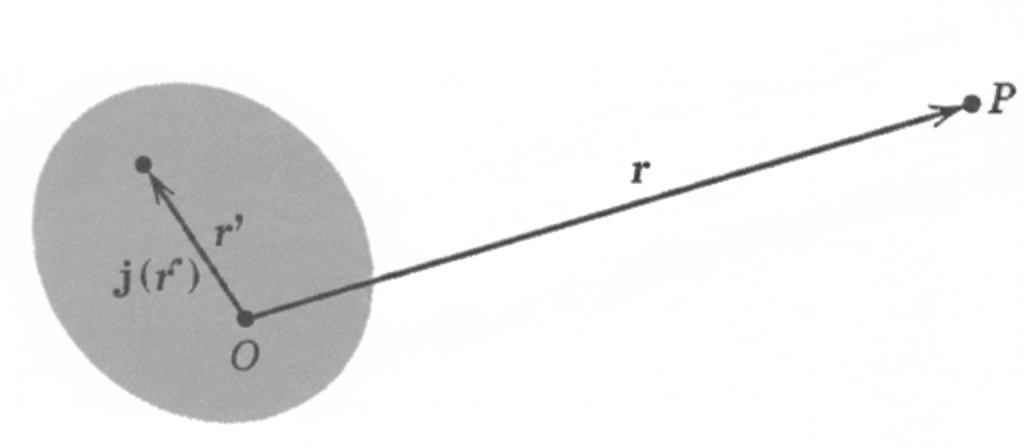
\includegraphics[width=0.5\linewidth]{figure/image49.png}
    \caption{Una distribuzione localizzata di corrente di densità $\mathbf{j} (\mathbf{r'})$ genera una distribuzione magnetica nel punto $P$ di coordinate $\mathbf{r}$}
    \label{fig:placeholder}
\end{figure}

Assumendo che $|\mathbf{r}| \gg |\mathbf{r'}|$, sviluppiamo il denominatore della \ref{eq:forma_esplicita_potenziale_vet} in serie di potenze di $\mathbf{r'}$:

\begin{equation}
    \frac{1}{|\mathbf{r} - \mathbf{r'}|} = \frac{1}{|\mathbf{r}|} + \frac{\mathbf{r} \cdot \mathbf{r'}}{|\mathbf{r}|^3} + ...
\end{equation}

Allora per ogni componente del potenziale vettore si potrà scrivere lo sviluppo

\begin{equation}
    A_i (\mathbf{r}) = \frac{\mu_0}{4 \pi} \left[ \frac{1}{|\mathbf{r}|} \int j_i (\mathbf{r'}) d^3 r' + \frac{\mathbf{r}}{|\mathbf{r}|^3} \cdot \int j_i (\mathbf{\mathbf{r'}} ) \mathbf{r'} d^3 r' + ... \right]
\end{equation}

Dato che stiamo considerando casi stazionari, dall'equazione di continuità \ref{eq:equazione_continuità}, si ha che $\nabla \cdot \mathbf{j} = 0$. \\

Possiamo andare a semplificare la predente forma sfruttando una relazione matematica, che però non dimostreremo.\\

Siano $f(\mathbf{r'})$ e $g(\mathbf{r'})$ due funzioni regolari di $\mathbf{r'}$, che specificheremo in seguito. Allora, essendo $\mathbf{j}(\mathbf{r'})$ localizzata e con divergenza nulla, vale la relazione

\begin{tcolorbox}[colback=yellow!10!white, colframe=orange!70!black, boxrule=0.8pt]
\begin{equation} \label{eq:relazione_dip_magn}
    \int (f \mathbf{j} \cdot \nabla' g + g \mathbf{j} \cdot \nabla ' f  + fg \nabla' \cdot \mathbf{j}) d^3 r' = 0
\end{equation}
\end{tcolorbox}

Ponendo $f = 1$, $g = x_i'$, dalla \ref{eq:relazione_dip_magn} con $\nabla' \cdot \mathbf{j} = 0$ si ricava 

\begin{equation*}
    \int j_i (\mathbf{r'}) d^3 r' = 0
\end{equation*}

Quindi \emph{il primo termine nello sviluppo è nullo}. \\

Ponendo $f = r_i'$ e $g = r_j '$, si ricava 

\begin{equation*}
    \int (r_i' j_j + r_j' j_i) d^3 r' = 0
\end{equation*}

Cioè 

\begin{equation*}
    \int r'_j j _i d^3 r' = - \int r'_i j_j d^3 r' 
\end{equation*}

Usando questa relazione si nota facilemnte che vale 

\begin{equation*}
    \int r_j' j_i d^3 r' = \frac{1}{2} \int (r_j' j_i- r_i' j_j) d^3 r' 
\end{equation*}

Riconoscendo il prodotto vettoriale 

\begin{equation*}
    r_j' j_i- r_i' j_j = \varepsilon_{ijk} (\mathbf{r'} \times \mathbf{j})_k
\end{equation*}

Quindi 

\begin{equation*}
    \int r_j' j_i d^3 r' = \frac{1}{2} \int \varepsilon_{ijk} (\mathbf{r'} \times \mathbf{j})_k d^3 r'
\end{equation*}

Allora l'integrale al secondo termine dell'espansione può essere trasformato 

\begin{align}
\mathbf{r} \cdot \int \mathbf{r'} \, j_i(\mathbf{r'}) \, d^3 r'
&= \sum_j r_j \int r'_j \, j_i(\mathbf{r'}) \, d^3 r' \\[6pt] \label{eq: integrale_momento_magnetico}
&= -\frac{1}{2} \sum_j r_j \int \left( r'_i j_j(\mathbf{r'}) - r'_j j_i(\mathbf{r'}) \right) d^3 r' \\[6pt]
&= -\frac{1}{2} \sum_{j,k} \varepsilon_{ijk} \, r_j \int \left( \mathbf{r'} \times \mathbf{j}(\mathbf{r'}) \right)_k \, d^3 r' \\[6pt]
&= -\frac{1}{2} \left[ \mathbf{r} \times \int \left( \mathbf{r'} \times \mathbf{j}(\mathbf{r'}) \right) d^3 r' \right]_i
\end{align}

Allora se vado a definite il \emph{momento magnetico} come \mkeyword{momento magnetico}

\begin{tcolorbox}[colback=yellow!10!white, colframe=orange!70!black, boxrule=0.8pt]
\begin{equation} \label{eq:momento_magnetico}
    \mathbf{m} = \frac{1}{2} \int\mathbf{r'} \times \mathbf{j}(\mathbf{r'}) d^3 r' 
\end{equation}
\end{tcolorbox}

Se andiamo a sostituire i risultati trovati nell'espansione, troncandola al secondo ordine si ottiene 

\begin{equation}
    \mathbf{A} (\mathbf{r}) = \frac{\mu_0}{4 \pi} \frac{\mathbf{m \times \mathbf{r}}}{|\mathbf{r}|^3}
\end{equation}

Questo è il termine non nullo di ordine più basso nello sviluppo di $\mathbf{A}$ per una distribuzione stazionaria di correnti localizzate. L'induzione magnetica $\mathbf{B}$ può essere calcolata a partire dalla definizione di potenziale vettoriale.

\begin{tcolorbox}[colback=yellow!10!white, colframe=orange!70!black, boxrule=0.8pt]
\begin{equation} \label{eq:campo_magnetico_dipolo}
    \mathbf{B = }\frac{\mu_0}{4 \pi r^3} \left[ 3 (\mathbf{m} \cdot \mathbf{u}_r) \mathbf{u}_r - \mathbf{m} \right]
\end{equation}
\end{tcolorbox}

Si nota, così, la somiglianza nella forma tra la \ref{eq:campo_magnetico_dipolo} e la \ref{eq:campo_dipolo}. \\

\section{Momento magnetico di una spira filiforme piana}

Se la corrente è costituita da una spira filiforme piana ma di forma arbitraria, il momento magnetico può essere espresso in modo molto semplice. Se $ d\mathbf{s}$ è l'elemento di linea del circuito $C$ percorso dalla corrente $i$, la \ref{eq:momento_magnetico} diventa 

\begin{equation}
    \mathbf{m} = \frac{i}{2} \oint_{C} \mathbf{r'} \times d \mathbf{s}
\end{equation}

Per una spira piana il momento magnetico è dunque perpendicolare al piano della spira. Poiché $|\mathbf{r'} \times d \mathbf{s}|/2 = d\Sigma$, dove $d \Sigma$ è l'area del triangolo elementare definito dai due estremi di $d \mathbf{s}$ e dall'origine, l'integrale di linea da l'area totale della spira. Perciò il momento magnetico può essere espresso come 

\begin{tcolorbox}[colback=yellow!10!white, colframe=orange!70!black, boxrule=0.8pt]
\begin{equation} 
    \mathbf{m} = i \Sigma \ \mathbf{u}_n
\end{equation}
\end{tcolorbox}

Dove $i$ è la corrente che scorre attraverso la spira, $\Sigma$ è l'area racchiusa dal filo e $\mathbf{u}_n$ è il versore ortogonale al piano su cui giace la spira e il cui verso si ottiene grazie alla regola della mano destra in base al verso in cui scorre la corrente.\\

\section{Dipolo magnetico elementare} 

Il risultato ottenuto mostra che, a grandi distanze, il potenziale vettore generato da una distribuzione stazionaria di correnti localizzate ha la forma

\begin{tcolorbox}[colback=yellow!10!white, colframe=orange!70!black, boxrule=0.8pt]
\begin{equation}
    \mathbf{A}(\mathbf{r}) = \frac{\mu_0}{4 \pi} \frac{\mathbf{m} \times \mathbf{r}}{r^3}
\end{equation}
\end{tcolorbox}

che dipende unicamente dal momento magnetico $\mathbf{m}$ della distribuzione.

Questo suggerisce di interpretare $\mathbf{m}$ come la quantità che caratterizza il comportamento del sistema a grandi distanze, in completa analogia con il momento di dipolo elettrico nel caso elettrostatico.\\

Si introduce quindi il concetto di \emph{dipolo magnetico} \mkeyword{dipolo magnetico} come un sistema fisico il cui campo magnetico, a grandi distanze, è descritto dalla \ref{eq:campo_magnetico_dipolo}.\\

\newpage

Il modello più semplice di dipolo magnetico è costituito da una spira circolare percorsa da corrente, sufficientemente piccola rispetto alle distanze di osservazione.

\begin{figure} [h]
    \centering
    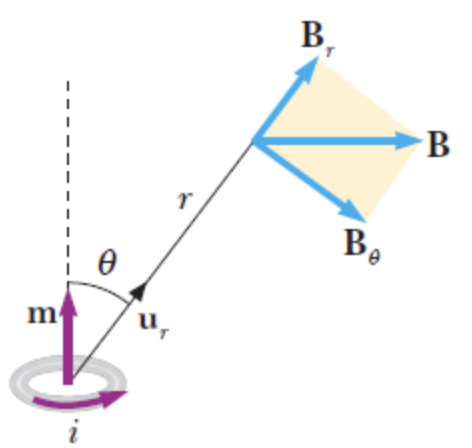
\includegraphics[width=0.5\linewidth]{figure/image50.png}
    \caption{Campo magnetico prodotto da un dipolo magnetico}
    \label{fig:placeholder}
\end{figure}

\section{Energia di un dipolo magnetico}

In analogia con quanto fatto con il dipolo elettrico, anche per il dipolo magnetico, spira o ago magnetico, si definisce un'energia potenziale, legata alla posizione angolare rispetto alla direzione di $\mathbf{B}$. \\

Consideriamo un dipolo magnetico immerso in un campo magnetico $\mathbf{B}$, la sua energia potenziale risulta essere 

\begin{tcolorbox}[colback=yellow!10!white, colframe=orange!70!black, boxrule=0.8pt]
\begin{equation}
    U_p = - \mathbf{m} \cdot \mathbf{B} = - mB \cos \theta = - i \Sigma B \cos \theta
\end{equation}
\end{tcolorbox}

A partire da questa definizione, allora, è possibile trovare anche un'espressione per la forza $\mathbf{F}$ che agisce sul dipolo. 

\begin{tcolorbox}[colback=yellow!10!white, colframe=orange!70!black, boxrule=0.8pt]
\begin{equation}
    \mathbf{F} = - \nabla U_p = \nabla (\mathbf{m} \cdot \mathbf{B})
\end{equation}
\end{tcolorbox}

\section{Momento meccanico di un dipolo magnetico}

In analogia con quanto fatto con il dipolo elettrico, anche per il dipolo magnetico, spira o ago magnetico, si definisce un momento meccanico, legato alla posizione angolare rispetto alla direzione di $\mathbf{B}$. \\

Consideriamo un dipolo magnetico immerso in un campo magnetico $\mathbf{B}$, il momento meccanico che agisce sul dipolo risulta essere 

\begin{tcolorbox}[colback=yellow!10!white, colframe=orange!70!black, boxrule=0.8pt]
\begin{equation}
    \mathbf{M} = \mathbf{m} \times \mathbf{B} = - m B \sin \theta \ \mathbf{u}_z = - \frac{\partial U_p}{\partial \theta} \ \mathbf{u}_z
\end{equation}
\end{tcolorbox}

\subsection{Interazione tra dipoli}

\section{Espressioni di forza, momento e lavoro tramite il flusso magnetico}

Consideriamo un circuito qualsiasi $C$, anche non piano, percorso dalla corrente $i$ e una qualsiasi superficie $\Sigma$ che abbia il circuito $C$ come contorno. Il circuito è immerso in un campo magnetico $\mathbf{B}$, anche non uniforme. \\

Estendiamo alla superficie $\Sigma$ l'argomento della suddivisione in tanti piccoli circuiti rettangolari, tutti percorsi dalla stessa corrente $i$ e concordemente orientati. 

\begin{figure} [h]
    \centering
    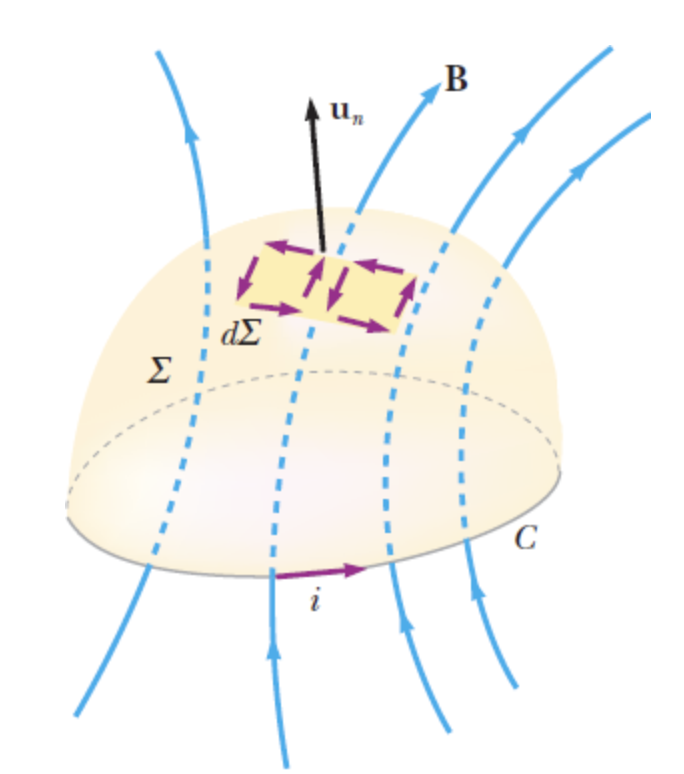
\includegraphics[width=0.5\linewidth]{figure/image51.png}
    \caption{}
    \label{fig:placeholder}
\end{figure}

L'energia potenziale del generico circuito di area $d\Sigma$ è 

\begin{equation*}
    d U_p = - d \mathbf{m} \cdot \mathbf{B} = - i \mathbf{B} \cdot \mathbf{u}_n \ d \Sigma = -i \ d\Phi (\mathbf{B})
\end{equation*}

dove $d \Phi (\mathbf{B})$ è il flusso infinitesimale di $\mathbf{B}$ attraverso $d \Sigma$. Integrando sulla superficie $\Sigma$ si ottiene l'energia potenziale del circuito $C$

\begin{tcolorbox}[colback=yellow!10!white, colframe=orange!70!black, boxrule=0.8pt]
\begin{equation}
    U_p = -i \int \mathbf{B} \cdot \mathbf{u}_n \ d \Sigma = -i \Phi (\mathbf{B})
\end{equation}
\end{tcolorbox}

L'energia potenziale di un circuito percorso da corrente $i$ e immerso in un campo magnetico $\mathbf{B}$ è eguale all'opposto del prodotto della corrente $i$ per il flusso di $\mathbf{B}$ concatenato col circuito.\\

Dato che $\mathbf{B}$ è solinoidale, il suo flusso non dipende dalla particolare $\Sigma$ che ha il circuito come contorno, ma solo dal contorno. 

A seguito di uno spostamento rigido o di una deformazione il flusso magnetico attraverso il circuito può cambiare e indichiamo con $d \Phi$ la variazione infinitesima di flusso. 
Nel processo viene compiuto, dalle forze del campo, il lavoro elementare

\begin{equation}
    dW = - dU_p = i \ d \Phi (\mathbf{B})
\end{equation}

Per una variazione finita da una configurazione iniziale 1 a una finale 2 il lavoro complessivo vale 

\begin{tcolorbox}[colback=yellow!10!white, colframe=orange!70!black, boxrule=0.8pt]
\begin{equation}
    W = i \Delta \Phi (\mathbf{B}) = i (\Phi_2 (\mathbf{B}) - \Phi_1 (\mathbf{B}))
\end{equation}
\end{tcolorbox}

\'E essenziale, per la validità delle formule trovate, che durante il processo la corrente resti costante.\\

Dalla relazione sopra, allora si ottiene che per una generica spira immersa in un campo magnetico vale 

\begin{tcolorbox}[colback=yellow!10!white, colframe=orange!70!black, boxrule=0.8pt]
\begin{equation}
    \mathbf{F} = i \nabla \Phi (\mathbf{B})
\end{equation}
\end{tcolorbox}

Mentre per il momento meccanico

\begin{tcolorbox}[colback=yellow!10!white, colframe=orange!70!black, boxrule=0.8pt]
\begin{equation}
    M = i \frac{\partial \Phi (\mathbf{B})}{\partial \theta} = - \frac{\partial U_p}{\partial \theta}
\end{equation}
\end{tcolorbox}


\chapter{Proprietà magnetiche della materia}

In questo capitolo andremo a trattare come i campi magnetici agiscono sui mezzi \\

Iniziamo dando una descrizione fenomenologica: consideriamo un solenoide rettilineo disposto con l'asse verticale e sospendiamo tramite una molla campioni di vari materiali aventi aventi piccole dimensioni. 

\begin{figure} [h]
    \centering
    \begin{subfigure}{0.45\textwidth}
        \centering
        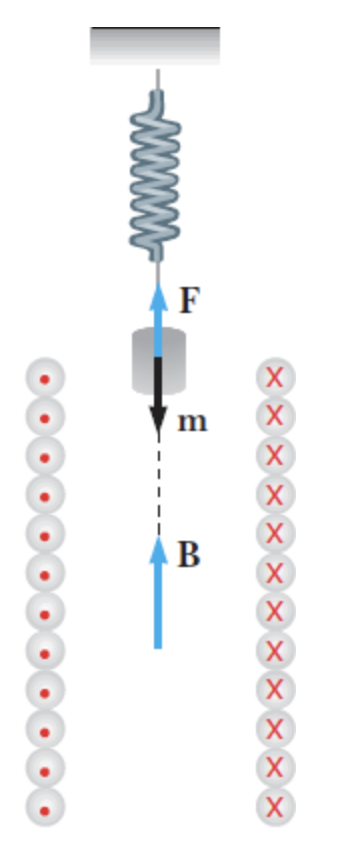
\includegraphics[width=0.5\linewidth]{figure/image52.png}
        \caption{Forza repulsiva}
        \label{fig:placeholder}
    \end{subfigure}
    \hfill
    \begin{subfigure}{0.45\textwidth}
        \centering
        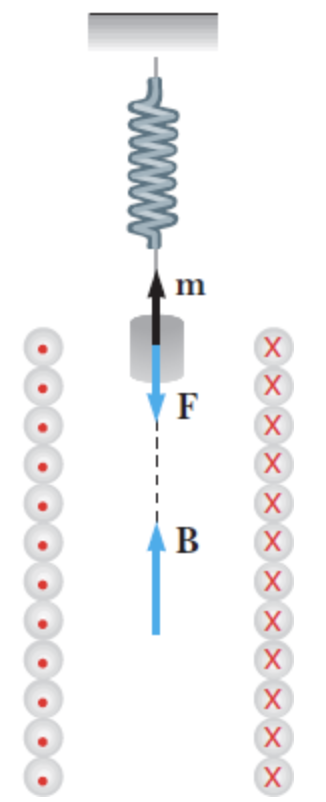
\includegraphics[width=0.5 \linewidth]{figure/image53.png}
        \caption{Forza attrattiva}
    \end{subfigure}
    \caption{Materiali sospesi soggetti al campo magnetico del solenoide}
\end{figure}

Quando nel solenoide circola corrente si osserva che su ciascun campione viene esercitata una forza. Alcuni campioni sono attratti verso l'interno, altri respinti verso l'esterno e ciò indipendentemente dal verso del campo magnetico. \\

Questo risultati si interpretano supponendo che alcune sostanze, sottoposte all'azione di un campo magnetico, acquistino un momento magnetico $\mathbf{m}$ parallelo e concorde a $\mathbf{B}$, mentre in altre $\mathbf{m}$ è parallelo e discorde a $\mathbf{B}$. \\

In base alle caratteristiche sperimentali descritte si può procedere a una suddivisione in tre classi alle quali, come vedremo in seguito, corrispondono diversi meccanismi microscopici di formazione del momento magnetico in presenza di un campo magnetico.

\begin{itemize}
    \item \emph{Sostanze diamagnetiche} \mkeyword{Sostanze diamagnetiche}
\end{itemize}

Sono dette diamagnetiche le sostanze che vengono respinte dal solenoide: la magnetizzazione è opposta al campo magnetico $\mathbf{B}$ esterno ed è ad esso proporzionale; l'effetto non dipende dalla temperatura, salvo poche eccezioni. È questa la classe più ampia a cui appartiene la maggior parte delle sostanze.

\begin{itemize}
    \item \emph{Sostanze paramagnetiche} \mkeyword{Sostanze paramagnetiche}
\end{itemize}

Si chiamano paramagnetiche le sostanze che vengono attratte dal solenoide, quelle cioè in cui la magnetizzazione è concorde al campo magnetico. Si trova che in generale l'effetto aumenta al diminuire della temperatura, ma ci sono svariate eccezioni. In tutti i casi si tratta di forze piuttosto piccole, alle temperature ordinarie.

\begin{itemize}
    \item \emph{Sostanze ferromagnetiche} \mkeyword{Sostanze ferromagnetiche}
\end{itemize}

Infine sono dette ferromagnetiche le sostanze che sono attratte fortemente verso la zona in cui il campo magnetico è maggiore; anche in questi campioni la magnetizzazione è concorde al campo magnetico, però la relazione tra $\mathbf{m}$ e $\mathbf{B}$ non è lineare e nemmeno univoca. Inoltre di norma i campioni rimangono magnetizzati anche dopo che il campo è stato rimosso, cosa che non accade con le sostanze diamagnetiche e paramagnetiche.

\section{Magnetizzazione}

In presenza di un campo magnetico, la materia si magnetizza, cioè gli atomi o le molecole del materiale acquistano sotto l'azione del campo $\mathbf{B}$ un momento magnetico medio $<\mathbf{m}>$ orientato parallelamente a $\mathbf{B}$. 

\begin{figure} [h]
    \centering
    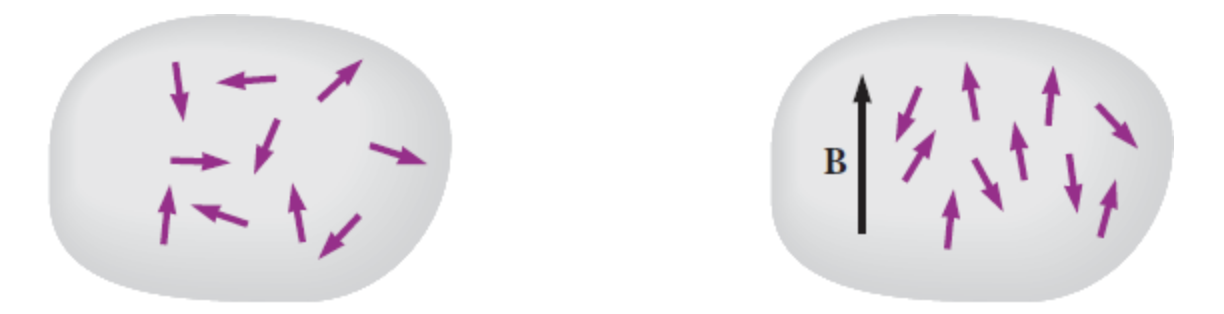
\includegraphics[width=0.8\linewidth]{figure/image54.png}
    \caption{Azione del campo magnetico sulle molecole di una sostanza}
    \label{fig:placeholder}
\end{figure}

Consideriamo un volumetto $\Delta \tau$ del materiale, contenente $\Delta N$ atomi (o molecole), il momento risultante è dato dal prodotto $\Delta N <\mathbf{m}>$ e il momento di dipolo magnetico per unità di volume è dato da 

\begin{equation}
    \mathbf{M} = \frac{\Delta N}{\Delta \tau} <\mathbf{m}>
\end{equation}

il vettore $\mathbf{M}$, che caratterizza l'effetto di formazione del momento di dipolo indotti dal campo esterno, si chiama \emph{magnetizzazione}. \\
In particolare se facciamo tendere $\Delta \tau$ a zero, otteniamo il valore di $\mathbf{M}$ in uno specifico punto del materiale.\\

$\mathbf{M}$ svolge un ruolo analogo alla polarizzazione $\mathbf{P}$ in elettrostatica. Nella sezione seguente, non ci preoccuperemo di come
la magnetizzazione si sia formata – potrebbe trattarsi di paramagnetismo, diamagnetismo o persino ferromagnetismo – ma prenderemo $\mathbf{M}$ come dato e calcoleremo il campo prodotto da questa magnetizzazione stessa.\\

Supponiamo di avere un pezzo di materiale magnetizzato, il momento di dipolo magnetico per unità di volume, $\mathbf{M}$, è noto. Troviamo quale campo magnetico è formato da questo oggetto. \\

Il potenziale vettore di un singolo dipolo $\mathbf{m}$ è dato da 

\begin{equation*}
    \mathbf{A} (\mathbf{r}) = \frac{\mu_0}{4 \pi} \frac{\mathbf{m} \times \mathbf{r}}{r^3}
\end{equation*}

Allora possiamo suddividere il materiale in un numero infinito di elementi, ciascuno con momento di dipolo $\mathbf{M} \ d \tau'$, quindi il potenziale vettore totale è 

\begin{equation}
    \mathbf{A} (\mathbf{r}) = \frac{\mu_0}{4 \pi} \int \frac{\mathbf{M} (\mathbf{r'}) \cdot \mathbf{u}_r}{r^2} d \tau'
\end{equation}

Questo in principio basterebbe, ma, come fatto nel capitolo dei dielettrici, l'integrale più essere riportato in una forma più conveniente usando l'identità 

\begin{equation*}
    \nabla' \left( \frac{1}{r} \right) = \frac{\mathbf{u}_r}{r^2}
\end{equation*}

Quindi 

\begin{equation*}
    \mathbf{A} (\mathbf{r}) = \frac{\mu_0}{4 \pi} \int \left[ \mathbf{M}(\mathbf{r}') \times \left( \nabla ' \frac{1}{r} \right) \right] d \tau'
\end{equation*}

Integrando per parti 

\begin{equation*}
    \mathbf{A} (\mathbf{r}) = \frac{\mu_0}{4\pi} \left\{ \int \frac{1}{r}[\nabla' \times \mathbf{M} (\mathbf{r'})] d \tau' - \int \nabla' \times \left[ \frac{\mathbf{M} (\mathbf{r'})}{r} \right] d \tau' \right\}
\end{equation*}

Applicando il teorema della divergenza per il secondo integrale 

\begin{equation*}
    \mathbf{A} (\mathbf{r}) = \frac{\mu_0}{4\pi} \int_{\tau}\frac{1}{r} [\nabla' \times \mathbf{M}(\mathbf{r'})] d \tau' + \frac{\mu_0}{4\pi} \oint_{\Sigma} \frac{1}{r} [\mathbf{M}(\mathbf{r'}) \times d \Sigma \  \mathbf{u}_n ] 
\end{equation*}

Si nota che il primo termine sembra il potenziale di un \mkeyword{densità volumica di corrente}volume di corrente con densità volumica di corrente 

\begin{tcolorbox}[colback=yellow!10!white, colframe=orange!70!black, boxrule=0.8pt]
\begin{equation}
    \mathbf{j}_m = \nabla \times \mathbf{M}
\end{equation}
\end{tcolorbox}

Mentre il secondo sembra il potenziale di una superficie \mkeyword{densità superficiale di corrente} di corrente con densità superficiale di corrente 

\begin{tcolorbox}[colback=yellow!10!white, colframe=orange!70!black, boxrule=0.8pt]
\begin{equation}
    \mathbf{K}_m = \mathbf{M} \times \mathbf{u}_n
\end{equation}
\end{tcolorbox}

Dove $\mathbf{u}_n$ è il vettore formale alla superficie in un punto. 

\newpage

\subsection{interpretazione fisica}

Abbiamo trovato che il campo di un oggetto magnetizzato è identico al campo che verrebbe prodotto da una certa distribuzione di correnti di densità $\mathbf{j}_m$ e $\mathbf{K}_m$. Andiamo a dare un significato fisico a questo risultato.\\

Questo sarà un argomento euristico - la derivazione rigorosa è già stata fornita. La Figura \ref{Figure:lasta_sottile} mostra una sottile lastra di materiale uniformemente magnetizzato, con i dipoli rappresentati come piccole spire di corrente. \\

\begin{figure} [h]
    \centering
    \begin{subfigure}{0.45\textwidth}
        \centering
        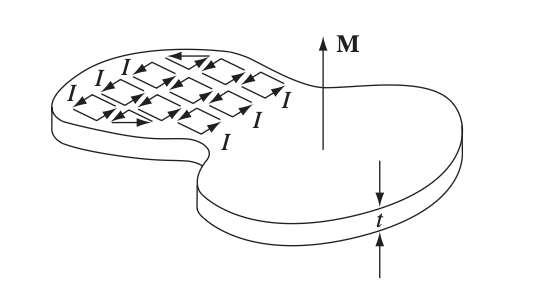
\includegraphics[width=1.0\linewidth]{figure/image55.png}
    \end{subfigure}
    \hfill
    \begin{subfigure}{0.45\textwidth}
        \centering
        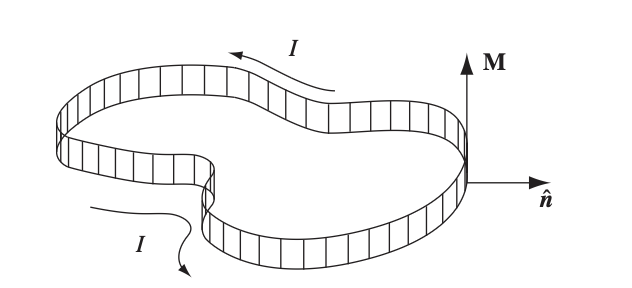
\includegraphics[width=1.0 \linewidth]{figure/image56.png}
    \end{subfigure}
    \caption{}
    \label{Figure:lasta_sottile}
\end{figure}

Se $\mathbf{M}$ è uniforme si nota che tutte le correnti interne si annullano: ogni volta che ce n'è una diretta verso destra, una contigua è diretta verso sinistra. Tuttavia, al bordo non c'è alcuna spira adiacente che possa effettuare la cancellazione. L'intero sistema è quindi equivalente a un unico nastro di corrente $i$ che scorre lungo il contorno.\\

\'E possibile esprimere questa corrente, in termini di $\mathbf{M}$. Supponiamo che ciascuna delle piccole spire abbia area $\Sigma$ e spessore $h$ . In termini della magnetizzazione $M$, il suo momento di dipolo è $m = M \ \Sigma h$. Tuttavia in termine della corrente $i$ vale $m = i \Sigma$. Quindi deve valere $i = Mh$ e quindi si ricava facilmente che 

\begin{equation}
    \mathbf{K}_m = \mathbf{M} \times \mathbf{u}_n
\end{equation}

Che è proprio quello che ci aspettavamo.\\

Quando la magnetizzazione è non uniforme, le correnti interne non si annullano più. 

\begin{figure} [h]
    \centering
    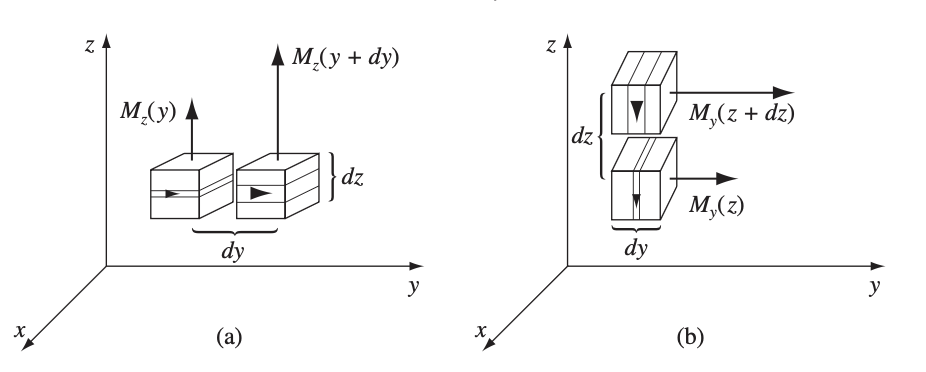
\includegraphics[width=0.75\linewidth]{figure/image58.png}
    \caption{}
    \label{fig:dipolo_non_unif}
\end{figure}

La Figura \ref{fig:dipolo_non_unif} mostra due porzioni adiacenti di materiale magnetizzato, con una freccia più grande su quella a destra che suggerisce una magnetizzazione maggiore in quel punto. Sulla superficie in cui esse si incontrano, c'è una corrente netta nella direzione $x$, data da

\[
i_x = \big[ M_z(y + dy) - M_z(y) \big] \, dz 
= \frac{\partial M_z}{\partial y} \, dy \, dz.
\]

La corrispondente densità di corrente volumica è quindi

\[
(j_m)_x = \frac{\partial M_z}{\partial y}.
\]

Allo stesso modo, una magnetizzazione non uniforme nella direzione $y$ contribuirebbe con un termine $-\partial M_y / \partial z$, per cui

\[
(j_m)_x = \frac{\partial M_z}{\partial y} - \frac{\partial M_y}{\partial z}.
\]

In generale, quindi,

\[
\mathbf{j}_m = \nabla \times \mathbf{M},
\]

in accordo, ancora una volta, con il risultato trovato sopra.

\section{Equazioni della magnetostatica nei mezzi}

Dal momento che il campo magnetico è solinoidale, anche in presenza di mezzi continuano a valere le due condizioni, integrale e locale, date da

\begin{equation*}
    \oint_{\Sigma} \mathbf{B} \cdot \mathbf{u}_n \ d\Sigma = 0 \quad , \quad \nabla \cdot \mathbf{B} = 0 
\end{equation*}

Anche la legge di Ampère rimane valida, \emph{purché si tenga conto delle correnti amperiane oltre che alle correnti di conduzione}:

\begin{tcolorbox}[colback=yellow!10!white, colframe=orange!70!black, boxrule=0.8pt]
\begin{equation}
        \oint \mathbf{B} \cdot d \mathbf{s} = \mu_0 (Ni + i_m)
\end{equation}
\end{tcolorbox}

Deduciamo la forma locale 

\begin{tcolorbox}[colback=yellow!10!white, colframe=orange!70!black, boxrule=0.8pt]
\begin{equation}
        \nabla \times \mathbf{B} = \mu_0 (\mathbf{j} + \mathbf{j}_m)
\end{equation}
\end{tcolorbox}

Allora si nota facilmente che 

\begin{equation}
    \frac{\nabla \times \mathbf{B}}{\mu_0} = \nabla \times \frac{\mathbf{B}}{\mu_0} = \mathbf{j} + \nabla \times \mathbf{M} \implies \nabla \times \left( \frac{\mathbf{B}}{\mu_0} - \mathbf{M} \right) = \mathbf{j}
\end{equation}

A cui corrisponde l'integrale 

\begin{equation}
    \oint \left( \frac{\mathbf{B}}{\mu_0} - \mathbf{M} \right) \cdot d \mathbf{s} = i
\end{equation}

\newpage

Allora possiamo andare a definire una nuova grandezza vettoriale 

\begin{tcolorbox}[colback=yellow!10!white, colframe=orange!70!black, boxrule=0.8pt]
\begin{equation}
        \mathbf{H} = \frac{\mathbf{B}}{\mu_0} - \mathbf{M}
\end{equation}
\end{tcolorbox}

Dove $\mathbf{H}$ prende il nome di \emph{campo magnetizzante}.  \mkeyword{campo magnetizzante}\\

Allora possiamo scrivere:

\begin{tcolorbox}[colback=yellow!10!white, colframe=orange!70!black, boxrule=0.8pt]
\begin{equation}
        \nabla \times \mathbf{H} = \mathbf{j} \quad , \quad \oint \mathbf{H} \cdot d\mathbf{s} = i
\end{equation}
\end{tcolorbox}

La circuitazione del vettore $\mathbf{H}$ lungo una linea chiusa è uguale alla somma delle correnti di conduzione concatenate con la linea; mentre il rotore del vettore $\mathbf{H}$ è uguale alla densità delle correnti di conduzione.\\

La circuitazione del vettore $\mathbf{H}$ non dipende dalla presenza del materiale magnetizzato. \\

\'E possibile trovare una relazione diretta tra $\mathbf{H}$ e $\mathbf{B}$ e tra $\mathbf{H}$ e $\mathbf{M}$. \\
Assumendo come relazione caratteristica 

\begin{tcolorbox}[colback=yellow!10!white, colframe=orange!70!black, boxrule=0.8pt]
\begin{equation}
        \mathbf{M} = \chi_m \mathbf{H} = (\kappa_m - 1) \mathbf{H}
\end{equation}
\end{tcolorbox}

Dove $\kappa_m$ prende il nome di \emph{permeabilità magnetica relativa del mezzo} \mkeyword{permeabilità magnetica relativa del mezzo}, mentre $\chi_m$ prende il nome di \emph{suscettività magnetica}. \mkeyword{suscettività magnetica}\\
Queste due grandezze \emph{dipendono solamente dalla natura del mezzo, indipendentemente dalla geometria e grandezza}. \\

Allora abbiamo come immediata conseguenza

\begin{tcolorbox}[colback=yellow!10!white, colframe=orange!70!black, boxrule=0.8pt]
\begin{equation}
        \mathbf{B} = \mu_0 \kappa_m \ \mathbf{H} = \mu \ \mathbf{H}
\end{equation}
\end{tcolorbox}

Dove $\mu$ è definito come il prodotto tra $\mu_0$ e $\kappa_m$ e prende il nome \emph{permeabilità magnetica assoluta}. \mkeyword{permeabilità magnetica assoluta}\\

\'E possibile trovare una relazione che leghi $\mathbf{M}$ e $\mathbf{B}$

\begin{tcolorbox}[colback=yellow!10!white, colframe=orange!70!black, boxrule=0.8pt]
\begin{equation}
        \mathbf{M} = \frac{\chi_m}{\mu} \ \mathbf{B} = \frac{1}{\mu_0} \frac{\chi_m}{\kappa_m} \mathbf{B} = \frac{1}{\mu_0} \frac{\kappa_m - 1}{\kappa_m} \mathbf{B}
\end{equation}
\end{tcolorbox}

\newpage

\section{Discontinuità dei campi sulla superficie di separazione tra due mezzi magnetizzati}

Prima di andare a vedere come si comporta un campo magnetico quando attraversa una superficie di separazione tra due mezzi con permeabilità magnetica diversa, vediamo come questo si comporta quando nell'attraversamento di una superficie sede di una corrente con densità lineare $\mathbf{K}_s$.  

\begin{figure}[h]
    \centering
    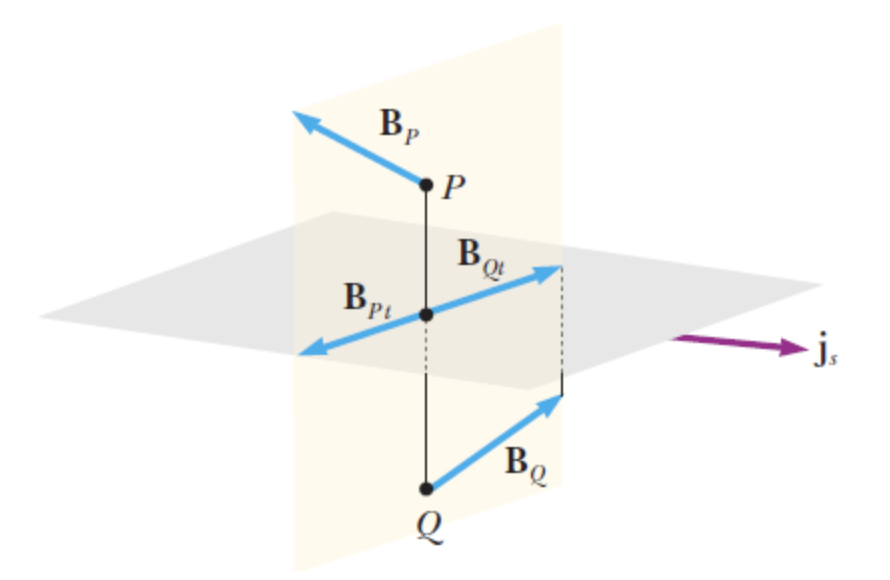
\includegraphics[width=0.7\linewidth]{figure/image59.png}
    \caption{}
    \label{fig:placeholder}
\end{figure}

Presi due punti $P$ e $Q$ molto vicini alla superficie, che quindi localmente appare piana, il campo magnetico dovuto alla corrente superficiale nei punti $P$ e $Q$ è dato dalla relazione 

\begin{equation}
    \mathbf{B} = \frac{\mu_0}{2} \mathbf{K}_s \times \mathbf{u} 
\end{equation}


A questo campo in generale si sovrappone un campo magnetico $\mathbf{B}$ dovuto ad altre sorgenti, che nei punti $P$ e $Q$ molto vicini tra loro ha lo stesso valore. Il campo magnetico totale nei due punti è pertanto diverso:

\begin{equation*}
    \mathbf{B}_P = \mathbf{B} + \frac{\mu_0}{2} \mathbf{K}_s \times \mathbf{u}_n \quad , \quad \mathbf{B}_Q = \mathbf{B} - \frac{\mu_0}{2} \mathbf{K}_s \times \mathbf{u}_n
\end{equation*}

La discontinuità è data da 

\begin{tcolorbox}[colback=yellow!10!white, colframe=orange!70!black, boxrule=0.8pt]
\begin{equation}
        \Delta \mathbf{B} = \mathbf{B}_P - \mathbf{B}_Q = \mu_0 \mathbf{K}_s \times \mathbf{u}_n
\end{equation}
\end{tcolorbox}

Quindi il campo magnetico varia nell'attraversamento di una densità lineare di corrente. \\

\newpage

\subsection{Discontinuità tra mezzi}

Vediamo come questo si comporta quando attraversa una superficie di separazione tra due materiali con permeabilità magnetica diversa.\\

Supponiamo di avere due mezzi con permeabilità magnetica relativa $\kappa_{m1}$ e $\kappa_{m2}$. Indichiamo con $\mathbf{H}_1$, $\mathbf{B}_1 = \mu_1 \mathbf{H}_1$ i campi nel primo mezzo e con $\mathbf{H}_2$, $\mathbf{B}_2 = \mu_2 \mathbf{H}_2$ e sia $\mathbf{u}_n$ la normale alla superficie di separazione nel punto $P$ considerato.\\

\begin{figure} [h]
    \centering
    \begin{subfigure}{0.45\textwidth}
        \centering
        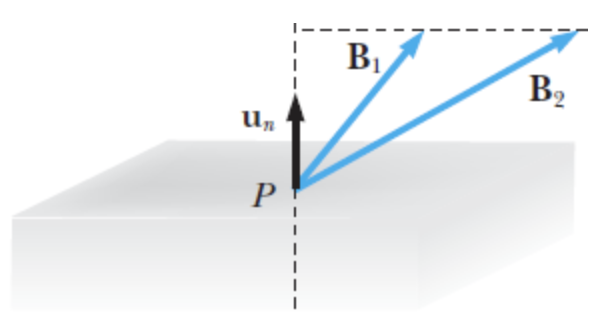
\includegraphics[width=0.80\linewidth]{figure/image60.png}
        \label{fig:placeholder}
    \end{subfigure}
    \hfill
    \begin{subfigure}{0.45\textwidth}
        \centering
        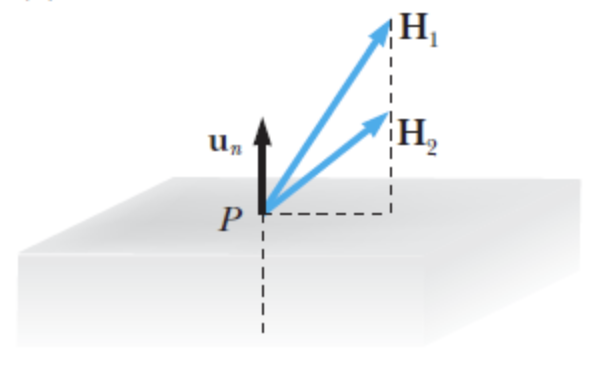
\includegraphics[width=0.80 \linewidth]{figure/image61.png}
    \end{subfigure}
    \caption{}
\end{figure}

Ammettiamo dunque che $\mathbf{H}_1$, $\mathbf{B}_1 = \mu_1 \mathbf{H}_1$, $\mathbf{H}_2$, $\mathbf{B}_2 = \mu_2 \mathbf{H}_2$ siano tutti in uno stesso piano che contiene la normale un alla superficie di separazione nel punto $P$ considerato.\\
L’applicazione della legge di Gauss del campo $\mathbf{B}$ ad una scatola cilindrica di altezza infinitesima, con le basi nei due mezzi e parallele alla superficie, porta alla relazione

\begin{tcolorbox}[colback=yellow!10!white, colframe=orange!70!black, boxrule=0.8pt]
\begin{equation}
        B_{1n} = B_1 \cos \theta_1 = B_2 \cos \theta_2 = B_{2n}
\end{equation}
\end{tcolorbox}

Cioè il campo magnetico $\mathbf{B}$ ha la stessa componente normale dalle due parti della superficie di separazione. \\
Da questa segue 

\begin{tcolorbox}[colback=yellow!10!white, colframe=orange!70!black, boxrule=0.8pt]
\begin{equation}
        \kappa_1 H_1 \cos \theta_1 = \kappa_2 H_2 \cos \theta _2
\end{equation}
\end{tcolorbox}

Applichiamo la legge di Ampère a un rettangolo che sta nel piano individuato dai campi, con due lati paralleli alla superficie di separazione e da parti opposte e gli altri due lati infinitesimi. Si trova

\begin{equation}
    \oint \mathbf{H} \cdot d \mathbf{s}  = H_{1t} h - H_{2t} h = 0
\end{equation}

non essendoci correnti di conduzione concatenate e quindi 

\begin{tcolorbox}[colback=yellow!10!white, colframe=orange!70!black, boxrule=0.8pt]
\begin{equation}
        H_1 \sin \theta_1 =  H_2 \sin \theta _2
\end{equation}
\end{tcolorbox}

Combinando i risultati ottenuti si ottiene

\begin{tcolorbox}[colback=yellow!10!white, colframe=orange!70!black, boxrule=0.8pt]
\begin{equation}
        \frac{\text{tg} \theta_1}{\text{tg}} = \frac{\kappa_{m1}}{\kappa_{m2}}
\end{equation}
\end{tcolorbox}

\section{Confronto tra le leggi dell'elettrostatica e della magnetostatica in mezzi omogenei indefiniti}

Abbiamo già notato varie volte nel corso di questo capitolo analogie con la trattazione delle proprietà dei dielettrici polarizzati. 
La ragione risiede nel fatto che, pur essendo fenomeni fisici diversi, le equazioni che li descrivono hanno la stessa struttura e quindi le soluzioni sono matematicamente eguali, anche se si riferiscono a campi diversi .\\

Per effetture il confronto dove è più appropriato, riscriviamo le equazioni generali dell'elettrostatica e della magnetostatica in mezzi indefiniti e in assenza di cariche elettriche libere ($\rho = 0$) e di correnti di conduzione ($\mathbf{j} = 0$):

\begin{tcolorbox}[colback=yellow!10!white, colframe=orange!70!black, boxrule=0.8pt]
\begin{equation}
\begin{array}{cc}
\nabla \times \mathbf{E} = 0 & \nabla \times \mathbf{H} = 0 \\[1.2em]
\nabla \cdot \mathbf{D} = 0 & \nabla \cdot \mathbf{B} = 0 \\[1.2em]
\dfrac{\mathbf{D}}{\varepsilon_0} = \mathbf{E} + \dfrac{\mathbf{P}}{\varepsilon_0}
&
\dfrac{\mathbf{B}}{\mu_0} = \mathbf{H} + \mathbf{M}
\end{array}
\end{equation}
\end{tcolorbox}

Queste mettono in evidenza le corrispondenze formali

\begin{tcolorbox}[colback=yellow!10!white, colframe=orange!70!black, boxrule=0.8pt]
\begin{equation}
    \mathbf{E} \leftrightarrow \mathbf{H} \quad , \quad \frac{\mathbf{D}}{\varepsilon_0} \leftrightarrow \frac{\mathbf{B}}{\mu_0}  \quad , \quad \frac{\mathbf{P}}{\varepsilon_0} \leftrightarrow \mathbf{M}
\end{equation}
\end{tcolorbox}

\newgeometry{
    a4paper,
    top=24mm,
    bottom=28mm,
    left=39mm,
    right=39mm,
    heightrounded
}
\partpage{Elettrodinamica}
\restoregeometry


\chapter{Legge di Faraday}

Le prime osservazione quantitative sulle relazioni fra campi elettrici e magnetici dipendenti dal tempo furono eseguite da Faraday (1831) mediante esperimenti sul comportamento delle correnti in circuiti immersi in campo magnetici variabili nel tempo. \\

Faraday osservò che si generano delle correnti transitorie nei segenti casi:

\begin{itemize}
    \item quando in un circuito adiacente viene accesa o spenta una corrente
    \item quando il circuito adiacente, con corrente costante, viene spostato rispetto al circuito in esame
    \item quando un magnete permanente viene avvicinato o allontanato rispetto al circuito in esame
\end{itemize}

Faraday attribuì la causa della corrente transitoria in tutti e tre i casi alla \emph{variazione del flusso magnetico concatenato al circuito in esame}: la variazione del flusso induce nel circuito un campo elettrico, la cui circuitazione viene chiamata forza elettromotrice indotta $\mathcal{E}$. \mkeyword{forza elettromotrice indotta}\\

Esprimiamo ora i risultati delle osservazioni di Faraday in forma matematica. Consideriamo un superficie $\Sigma$, con versore ortogonale $\mathbf{u}_n$, che abbia il circuito $C$ come contorno. Sia $\mathbf{B}$ il campo magnetico nella regione occupata dal circuito; il flusso magnetico concatenato è definito dalla formula:

\begin{equation}
\Phi (\mathbf{B}) = \int_{\Sigma} \mathbf{B} \cdot \mathbf{u}_n \, d\Sigma
\end{equation}

La forza elettromotrice lungo il circuito è definta come 

\begin{equation}
    \mathcal{E} = \oint_C \mathbf{E'} \cdot d\mathbf{l}
\end{equation}

dove $\mathbf{E}'$ è il campo elettrico indotto in corrispondenza dell'elemento $d \mathbf{l}$ di $C$. \\

I risultati delle osservazioni di Faraday sono riassunti nella forma

\begin{tcolorbox}[colback=yellow!10!white, colframe=orange!70!black, boxrule=0.8pt]
\begin{equation} \label{eq: Legge di Faraday}
\mathcal{E} = -\frac{d\Phi (\mathbf{B})}{dt}
\end{equation}
\end{tcolorbox}

Questa relazione prende il nome di \emph{Legge di Faraday}. \mkeyword{Legge di Faraday} \\

\newpage

\subsection{Legge di Lenz}

Il segno meno che compare nella \ref{eq: Legge di Faraday} è molto importante e viene messo in evidenza con un enunciato particolare, detto \emph{legge di Lenz}: l'effetto della forza elettromotrice indotta è sempre tale da opporsi alla causa che ha generato il fenomeno. \\

Ad esempio, se in un circuito chiuso circola una corrente indotta, questa ha verso tale che il flusso del proprio campo magnetico concatenato col circuito si oppone alla variazione del flusso primario $\Phi$.\\

Questo comportamento è in accordo con il principio di conservazione dell'energia. 

\section{Invarianza sotto trasformazioni di Galileo}

Prima dello sviluppo della relatività speciale (e anche dopo, nei casi in cui si ha a che fare con velocità relative piccole rispetto alla velocità della luce) tutti i fisici erano concordi nel ritenere che tutte le leggi fisiche dovessero essere invarianti rispetto a trasformazioni di Galieleo. \\

Ciò significa che tutti i fenomeni fisici devono apparire identici a due osservatori che si muovono l'uno rispetto all'altro con velocità relativa $\mathbf{v}$ costante.\\

Consideriamo ora la legge di Faraday per un circuito (secondario) in moto e vediamo le conseguenze dell'invarianza galileiana. \\
Esprimendo la \ref{eq: Legge di Faraday} madiante integrali dei campo $\mathbf{E}'$ e $\mathbf{B}$, si ha 

\begin{equation} \label{eq: L. Faraday integrale}
    \oint_C \mathbf{E'} \cdot d \mathbf{l} = - \int_{\Sigma} \mathbf{B} \cdot \mathbf{u}_n \ d\Sigma
\end{equation}

La linea di integrazione può essere pensata come una linea geometrica chiusa qualsiasi, non necessariamente materializzata da un filo conduttore, e la \ref{eq: Legge di Faraday} diventa così una relazione generale fra i campi. \\

\' E tuttavia importante notare che il campo elettrico $\mathbf{E}'$ è il campo elettrico nel punto in cui si trova l'elemento $d \mathbf{l}$, misurato nel sistema di coordinate in cui $d \mathbf{l}$ è in quiete.\\

Se il circuito $C$ si muove con velocità $\mathbf{v}$ in un certa direzione, la derivata temporale totale che compare nella \ref{eq: Legge di Faraday} deve tener conto anche di questo movimento. 

\begin{figure} [h]
    \centering
    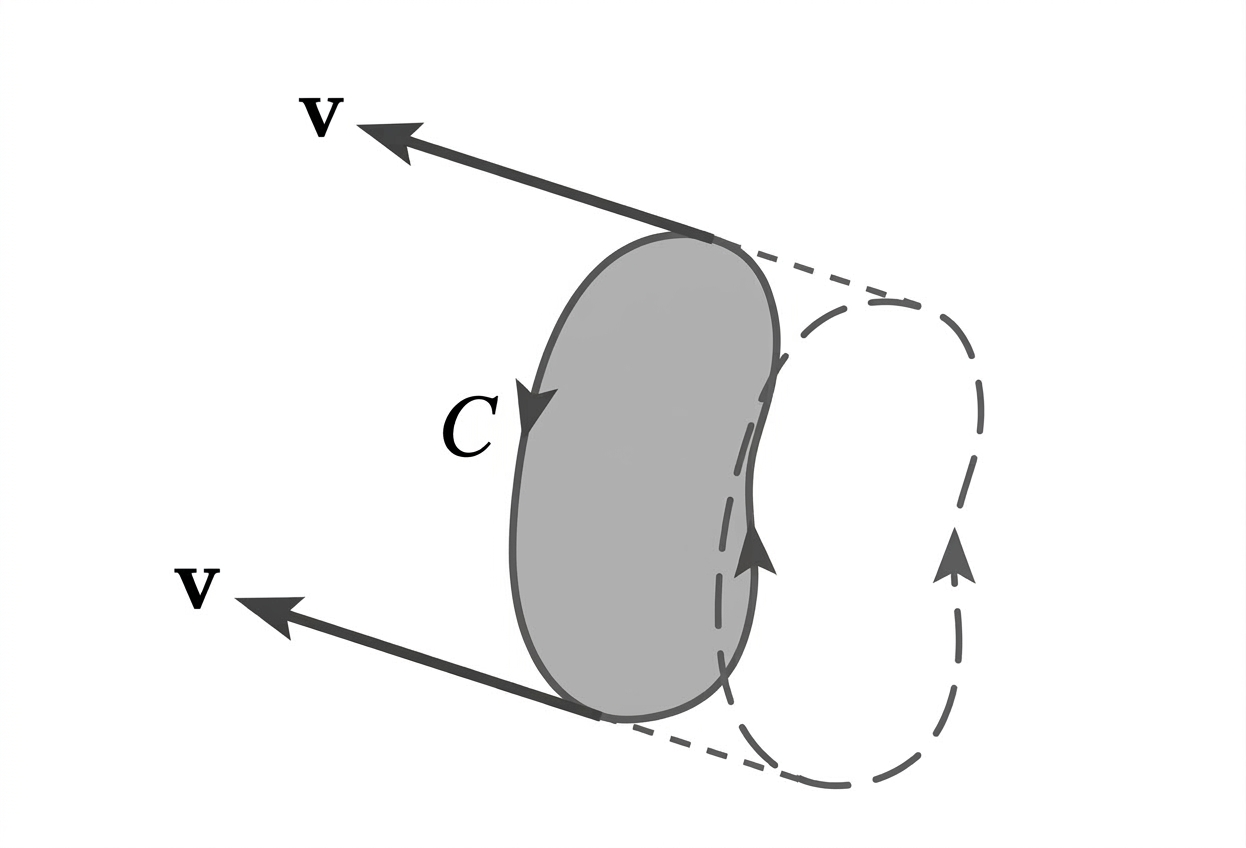
\includegraphics[width=0.4\linewidth]{figure/image63.png}
    \caption{}
\end{figure}

Il flusso concatenato nel sistema può variare perché:

\begin{itemize}
    \item varia col tempo il valore di $\mathbf{B}$ in tutti o in qualche punto.
    \item il movimento del circuito fa cambiare nel tempo la posizione del contorno. 
\end{itemize}

\newpage

\' E facile dimostrare che la derivata temporale totale del flusso concatenato si può scrivere nella forma 

\begin{equation}
    \frac{d}{dt} \int_{\Sigma} \mathbf{B} \cdot \mathbf{u}_n \ d \Sigma = \int_{\Sigma} \frac{\partial \mathbf{B}}{\partial t} \cdot \mathbf{u}_n \ d \Sigma + \oint_C (\mathbf{B} + \mathbf{v}) \cdot d \mathbf{l}
\end{equation}

L'equazione \ref{eq: L. Faraday integrale} può essere riscritta nella forma 

\begin{equation}
    \oint_C \left[ \mathbf{E'} - (\mathbf{v} \times \mathbf{B}) \right] \cdot d \mathbf{l} = - \int_{\Sigma} \frac{\partial \mathbf{B}}{\partial t} \cdot \mathbf{u}_n \ d\Sigma
\end{equation} 

Questo non è altro che una diversa enunciazione della legge di Faraday applicata al circuito in moto $C$. Ma possiamo anche interpretarla diversamente. Possiamo considerare il circuito $C$ e la superficie $\Sigma$ come situati, ad un certo istante, in una posizione fissa rispetto al sitema del laboratorio. Apllicando la legge di Faraday \ref{eq: Legge di Faraday} a questo circuito fissato, possiamo scrivere

\begin{equation}
    \oint_C \mathbf{E} \cdot d \mathbf{l} = - \int_{\Sigma} \frac{\partial \mathbf{B}}{\partial t} \cdot \mathbf{u}_n \ d\Sigma 
\end{equation}

Dove $\mathbf{E}$ è il campo elettrico misurato nel sistema del laboratorio. L'ipotesi di invarianza galileiana implica che i primi membri delle due equazioni devono essere uguali. 
Ciò significa che il campo elettrico $\mathbf{E}'$, misurato nel sistema di coordinate in moto, deve soddisfare 

\begin{tcolorbox}[colback=yellow!10!white, colframe=orange!70!black, boxrule=0.8pt]
\begin{equation} 
    \mathbf{E}' = \mathbf{E} + (\mathbf{v} \times \mathbf{B})
\end{equation}
\end{tcolorbox}

\subsection{Forma diffenziale della legge di Faraday}

Ma allora la legge di Faraday può essere posta in forma differenziale  usando il teorema di Stokes, purché il circuito cosiderato sia fisso nel sistema di riferimento scelto. Trasformando l'integrale che esprime la forza elettromotrice in un intrgrale di superficie si ottiene

\begin{equation}
    \int_{\Sigma} \left( \nabla \times \mathbf{E} + \frac{\partial \mathbf{B}}{\partial t}  \right) \cdot \mathbf{u}_n \ d\Sigma = 0
\end{equation}

Dato che il contorno $C$ e la superficie $\Sigma$ sono arbitrari, l'integrando deve essere nullo ovunque. \\

\newpage

Pertanto, la forma differenziale dell alegge di Faraday è 

\begin{tcolorbox}[colback=yellow!10!white, colframe=orange!70!black, boxrule=0.8pt]
\begin{equation} 
    \nabla \times \mathbf{E} = - \frac{\partial \mathbf{B}}{\partial t}
\end{equation}
\end{tcolorbox}

Notiamo che questa non è altro che l'estensione, al caso di campi dipendenti dal tempo, della proprietà $\nabla \times \mathbf{E} = 0$ valida per i campi elettrici statici. 

\section{Autoinduzione}

Un circuito di forma qualunque percorso da corrente produce un campo magnetico secondo la legge di Ampère-Laplace.
Il flusso di questo campo concatenato col circuito stesso, detto \emph{autoflusso} \mkeyword{autoflusso}, è dato da:

\begin{equation*}
    \Phi(\mathbf{B}) = \int_{\Sigma} \left( \oint_{C} \frac{\mu_0 i}{4 \pi} \frac{d \mathbf{s} \times \mathbf{u}_r}{r^2} \right) \cdot \mathbf{u}_n \ d\Sigma
\end{equation*}

dove $\Sigma$ è una qualunque superficie che abbia come contorno $C$. Sia il campo magnetico che, di conseguenza, il flusso del campo magnetico sono proporzionali alla corrente e si sfrutta questa proprietà per scrivere l'autoflusso come

\begin{tcolorbox}[colback=yellow!10!white, colframe=orange!70!black, boxrule=0.8pt]
\begin{equation} 
    \Phi (\mathbf{B}) = L i 
\end{equation}
\end{tcolorbox}

Il fattore $L$ si chiama coefficiente di autoinduzione o induttanza \mkeyword{induttanza} del circuito. Esso dipende dalla forma del circuito e dalle proprietà magnetiche del mezzo. 

\subsection{Forza elettromotrice di autoinduzione}

La nozione di autoflusso acquista particolare importanza quando la corrente nel circuito non è costante nel tempo oppure quando viene variata la forma del circuito. 
In entrambi i casi, come nel caso più generale in cui le due variazioni avvengano contemporaneamente, il flusso concatenato col circuito cambia nel tempo e nel circuito compare una f.e.m. indotta che con i suoi effetti tende ad opporsi alla variazione che l’ha generata. 
Tale forza elettromotrice, detta di autoinduzione, si calcola usando la \ref{eq: Legge di Faraday}:

\begin{equation}
    \mathcal{E}_L = - \frac{d \Phi}{dt} = - \frac{d}{dt} (Li)
\end{equation}

Nei casi pratici più comuni il coefficiente di autoinduzione resta costante e assume la forma

\begin{tcolorbox}[colback=yellow!10!white, colframe=orange!70!black, boxrule=0.8pt]
\begin{equation} 
    \mathcal{E}_L = - L \frac{di}{dt}
\end{equation}
\end{tcolorbox}

\newpage

\section{Mutua indunzione}

Supponiamo di considerare due circuiti, allora si definisce il flusso del campo magentico prodotto dal primo circuito attraverso il secondo come 

\begin{equation}
    \Phi_{1,2} = \int_{\Sigma_2} \mathbf{B}_1 \cdot \mathbf{u}_n \ d\Sigma_2 
\end{equation}

dove $\Sigma_2$ è una qualunque superficie che si appoggia sul secondo circuito.
Dal momemento che $B_1$ è proporzionale a $i_1$ prossiamo scrivere

\begin{tcolorbox}[colback=yellow!10!white, colframe=orange!70!black, boxrule=0.8pt]
\begin{equation}
    \Phi_{1,2} = M_{1,2} i_1
\end{equation}
\end{tcolorbox}

conglobando in $M_{1,2}$ tutti i fattori geometrici e l'eventuale dipendenza dalle proprietà magnetiche del mezzo in cui sono immersi i circuiti. \\

In modo analogo si trova che il flusso del campo magnetico del secondo circuito attraverso il primo è 

\begin{tcolorbox}[colback=yellow!10!white, colframe=orange!70!black, boxrule=0.8pt]
\begin{equation}
    \Phi_{2,1} = M_{2,1} i_2
\end{equation}
\end{tcolorbox}

Un risultato molto importante (che però non andremo a dimostrare) e utile nella risoluzione di problemi è che vale l'uguaglianza 

\begin{tcolorbox}[colback=yellow!10!white, colframe=orange!70!black, boxrule=0.8pt]
\begin{equation}
    M_{1,2} = M_{2,1}
\end{equation}
\end{tcolorbox}

\subsection{Circuiti accoppiati}

Come per il fenomeno dell'autoinduzione, anche quello della mutuainduzione diventa fondamentale quando si ha variazione di corrente e quindi una variazione del flusso.\\

Supponendo che $M$ sia costante, si ha per le forze elettromotrici indotte in un circuito dallla variazione di corrente nell'altro

\begin{equation}
    \mathcal{E}_1' = - \frac{d \Phi_{2,1}}{dt} = - M \frac{di_2}{dt} \quad , \quad \mathcal{E}_2' = - \frac{d \Phi_{1,2}}{dt} = - M \frac{di_1}{dt}
\end{equation}

Queste vanno sommate in ciascun circuito alle forze elettromotrici di autoinduzione ottenendo in questo modo, applicando la seconda legge di Kirchoff e supponendo che in uno dei due circuiti ci sia un generatore:

\begin{tcolorbox}[colback=yellow!10!white, colframe=orange!70!black, boxrule=0.8pt]
\begin{align*}
    \mathcal{E}(t) - L_1 \frac{di_1}{dt} - M \frac{di_2}{dt} = R_1 i_1 \\
    - L_2 \frac{di_2}{dt} - M \frac{di_1}{dt} = R_2 i_2
\end{align*}
\end{tcolorbox}

Vediamo che la presenza di una corrente $i_2$ nel circuito senza generatore è possibile proprio grazie al processo di mutua induzione.



\chapter{Legge di Ampère-Maxwell}

Nei capitoli precedenti abbiamo trovato un'importante relazione tra il campo magnetico $\mathbf{B}$ e la corrente concatenata:

\begin{align}
    \oint_{C} \mathbf{B} \cdot d \mathbf{s} = \mu_0 i \\
    \nabla \times \mathbf{B} = \mu_0 \mathbf{j}
\end{align}

Questa relazione (riportata sia in forma integrale che differenziale) prende il nome di Legge di Ampère. \\

Quando abbiamo ricavato questa legge, però, abbiamo supposto di essere nel caso stazionario in cui $\nabla \cdot \mathbf{j} = 0$. Tuttavia nel caso generale vale l'equazione di continuità 

\begin{equation*}
    \nabla \cdot \mathbf{j} = - \frac{\partial \rho}{\partial t}
\end{equation*}

La quale, però, è in disaccordo con la legge di Ampère, infatti

\begin{equation}
    \nabla \cdot \mathbf{j} = \nabla \cdot \nabla \times \mathbf{B} = 0 \neq - \frac{\partial \rho}{\partial t}
\end{equation}

Ci è voluto il genio di J. C. Maxwell, stimolato dalle osservazioni di Faraday, per identificare la contraddizione e per modificare la legge di Ampère in una nuova legge che implica nuovi fenomeni, allora sconosciuti, ma in seguito osservati e verificati in dettaglio con gli esperimenti.\\

Ciò che Maxwell ha notato è il fatto che l'equazione di continuità si può convertire in una divergenza nulla usando la legge di Gauss, ossia 

\begin{equation}
    \nabla \cdot \mathbf{j} + \frac{\partial \rho}{\partial t} = \nabla \cdot \left( \mathbf{j} + \varepsilon_0 \frac{\partial \mathbf{E}}{\partial t} \right) = 0
\end{equation}

Maxwell ha quindi sostituito $\mathbf{j}$ nella legge di Ampère con la sua generaliazione 

\begin{tcolorbox}[colback=yellow!10!white, colframe=orange!70!black, boxrule=0.8pt]
\begin{equation}
    \mathbf{j} \to \mathbf{j} + \varepsilon_0\frac{\partial \mathbf{E}}{\partial t}
\end{equation}
\end{tcolorbox}

per campi dipendenti dal tempo. Pertanto le legge di Ampère si trasforma nella \emph{legge di Ampère-Maxwell} che diventa dunque 

\begin{tcolorbox}[colback=yellow!10!white, colframe=orange!70!black, boxrule=0.8pt]
\begin{equation}
    \nabla \times \mathbf{B} = \mu_0 \left( \mathbf{j} + \varepsilon_0 \frac{\partial \mathbf{E}}{\partial t} \right)
\end{equation}
\end{tcolorbox}

\newpage

mentre in foma integrale 

\begin{tcolorbox}[colback=yellow!10!white, colframe=orange!70!black, boxrule=0.8pt]
\begin{equation}
    \oint_{C} \mathbf{B} \cdot d \mathbf{s} = \mu_0 \int \left( \mathbf{j} + \varepsilon_0 \frac{\partial \mathbf{E}}{\partial t} \right) \cdot \mathbf{u}_n \ d\Sigma = \mu_0 (i + i_s) 
\end{equation}
\end{tcolorbox}

Dove $i_s$ è la corrente che si ottiene facendo l'integrale di superficie del primo termine e prende il nome di \emph{corente di spostamento}. \mkeyword{corrente di spostamento}

\section{Simmetria con la legge di Faraday}

Andiamo a considerare una regione di spazio in cui non ci sono correnti di conduzione ($i = 0$), ma ci sono variazioni di campo elettrico nel tempo, allora esiste un campo magnetico $\mathbf{B}$, determinato da 

\begin{tcolorbox}[colback=yellow!10!white, colframe=orange!70!black, boxrule=0.8pt]
\begin{equation}
    \oint_{C} \mathbf{B} \cdot d \mathbf{s} = \int_{\Sigma} \varepsilon_0 \mu_0 \frac{\partial \mathbf{E}}{\partial t} \cdot \mathbf{u}_n \ d\Sigma = \frac{1}{c^2} \frac{d \Phi (\mathbf{E})}{dt}
\end{equation}
\end{tcolorbox}

Dove abbiamo ulizzato l'espressione 

\begin{tcolorbox}[colback=yellow!10!white, colframe=orange!70!black, boxrule=0.8pt]
\begin{equation}
    c^2 = \frac{1}{\varepsilon_0 \mu_0}
\end{equation}
\end{tcolorbox}

Questo aspetto della legge di Ampère-Maxwell stabilisce una simmetria di comportamento con la legge di Faraday che prevede l'esistenza di un campo elettrico ove esistono variazioni di campo magnetico. 

\begin{figure}[h]
    \centering
    \begin{subfigure}{0.48\textwidth}
        \centering
        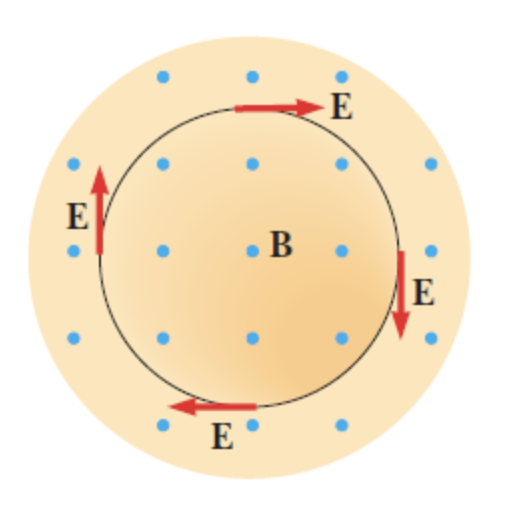
\includegraphics[width=0.7\linewidth]{figure/image64.png}
        \caption{$\oint_{C} \mathbf{E} \cdot d \mathbf{s} = - \frac{d \Phi(\mathbf{B})}{dt}$}
        \label{fig:sub1}
    \end{subfigure}
    \hfill
    \begin{subfigure}{0.48\textwidth}
        \centering
        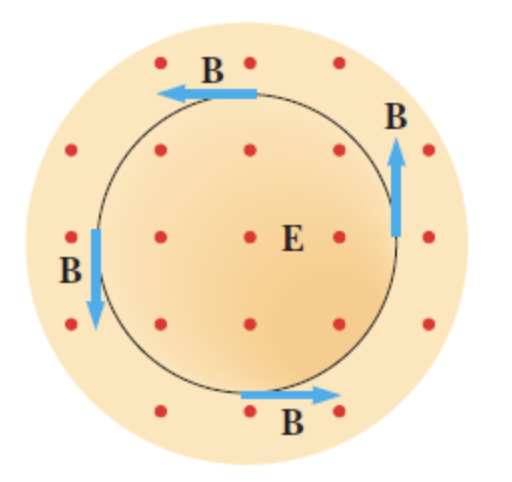
\includegraphics[width=0.7\linewidth]{figure/image65.png}
        \caption{$\oint_{C} \mathbf{B} \cdot d \mathbf{s} = \frac{1}{c^2} \frac{d \Phi(\mathbf{E})}{dt}$}
        \label{fig:sub2}
    \end{subfigure}
    %\caption{Confronto tra due campi elettrici}
    \label{fig:campi}
\end{figure}

\section{Campi magnetici quasi-statici ed effetto pelle} 

\chapter{Equazioni di Maxwell}

Nei capitoli precedenti abbiamo trattato principalmente problemi stazionari di elettricità e magentismo. Le tecniche matematiche utilizzate erano simili, ma i fenomeni elettrici e magnetici sono stati trattati come indipendenti.
L'unico legame fra di essi era nel fatto che le correnti che producono campi magnetici, essendo cariche in movimento, sono di natura essenzialmente elettrica.\\

La natura quasi indipendente dei fenomeni elettrici e magnetici scompare quando si considerano problemi in cui vi è una dipendenza dal tempo. La scoperta dell'induzione da parte di Faraday ha distrutto questa indipendenza. 
Campi magnetici variabili nel tempo danno origine a campi elettrici e viceversa. 
Dobbiamo allora parlare di \emph{campi elettromagnetici} piuttosto che di campi elettrici o magnetici. \\

L'importanza dell'interconnessione fra campi elettrici e magnetici e della loro essenziale unità si può comprendere chiaramente ed in modo completo solo nell'ambito della teoria della relatività speciale.
Per il momento ci accontenteremo di esaminare i fenomeni fondamentali e di dedurre l'insieme di equazioni noto come equazioni di Maxwell, che descrive il comportamento dei campi elettromagnetici. Verranno poi discussi i potenziali vettore e scalare, le trasformazioni di gauge, e le funzioni di Green per l'equazione d'onda, incluse le soluzioni ritardate per i campi come pure per i potenziali. 
Seguirà una derivazione delle equazioni dell'elettromagnetismo macroscopico. Verranno trattate infine le leggi di conservazione dell'energia e dell'impulso e le proprietà di trasformazione delle quantità elettromagnetiche ed anche l'interessante argomento dei monopoli magnetici.

\section{Le equazioni di Maxwell}

Le leggi fondamentali dell'elettricità o del magnetismo che abbiamo discusso fino ad ora possono essere riassunte in forma differenziale dalle seguenti quattro equazioni che prendono il nome di \emph{equazioni di Maxwell}: \mkeyword{equazioni di Maxwell}

\begin{tcolorbox}[colback=yellow!10!white, colframe=orange!70!black, boxrule=0.8pt]
\begin{align} \label{eq: Equazioni_di_Maxwell}
\text{Legge di Gauss} & \qquad \nabla \cdot \mathbf{E} = \frac{\rho}{\varepsilon_0} \\
\text{Assenza di poli magnetici liberi} & \qquad \nabla \cdot \mathbf{B} = 0 \\
\text{Legge di Faraday} & \qquad \nabla \times \mathbf{E} = - \frac{\partial \mathbf{B}}{\partial t} \\
\text{Legge di Ampère - Maxwell } & \qquad \nabla \times \mathbf{B} = \mu_0 \left( \mathbf{j} + \varepsilon_0 \frac{\partial \mathbf{E}}{\partial t} \right)
\end{align}
\end{tcolorbox}

\newpage

Queste equazioni formano la base di tutti i fenomeni elettromagnetici classici. \\

Combinato con l'equazione per la forza di Lorentz e la seconda legge del moto di Newton, questo insieme di equazioni fornisce una descrizione \emph{completa} della dinamica classica delle particelle cariche in interazione con il campo elettromagnetico. 

\section{Il potenziale vettore e il potenziale scalare}

Le equazioni di Maxwell sono un sistema di equazioni alle derivate parziali del primo ordine che legano le varie componenti dei campi elettrico e magnetico. 
In situazioni semplici esse possono essere risolte così come sono. \'E però spesso conveniente introdurre dei potenziali che risolvono identicamente alcune delle equazioni di Maxwell per ottenere un numero minore di equazioni di secondo ordine. \\

Abbiamo già familiarizzato con questo concetto in elettrostatica e in magnetostatica , dove abbiamo utilizzato il potenziale scalre $V$ (che adesso andremo a chiamare $\phi$) e il potenziale vettore $\mathbf{A}$. \\
Poiché $\nabla \cdot \mathbf{B} = 0$ è ancora valida, possiamo definire $\mathbf{B}$ in termini di un potenziale vettore:

\begin{tcolorbox}[colback=yellow!10!white, colframe=orange!70!black, boxrule=0.8pt]
\begin{equation}
    \mathbf{B} = \nabla \times \mathbf{A}
\end{equation}
\end{tcolorbox}

L'altra equazione omogenea nella \ref{eq: Equazioni_di_Maxwell}, la legge di Faraday, si può allora scrivere 

\begin{equation} \label{eq: Legge_di_Faraday_con_potenziali}
    \nabla \times \left(\mathbf{E} + \frac{\partial \mathbf{A}}{\partial t} \right) = 0
\end{equation}

Questo significa che la quantità a rotore nullo nella \ref{eq: Legge_di_Faraday_con_potenziali} si può scrivere come il gradiente di una qualche funzione scalare, ossia, un potenziale scalare $\phi$:

\begin{equation}
    \mathbf{E} + \frac{\partial \mathbf{A}}{\partial t} = - \nabla \phi
\end{equation}

oppure 

\begin{tcolorbox}[colback=yellow!10!white, colframe=orange!70!black, boxrule=0.8pt]
\begin{equation}
    \mathbf{E} = - \nabla \phi - \frac{\partial \mathbf{A}}{\partial t}
\end{equation}
\end{tcolorbox}

Le definizioni di $\mathbf{B}$ ed $\mathbf{E}$ in termini dei potenziali $\mathbf{A}$ e $\phi$ sono tali da soddisfare identicamente le due equazioni di Maxwell omogenee. Il comportamento dinamico di $\mathbf{A}$ e $\phi$ sarà determinato dalle due equazioni non omogenee nella \ref{eq: Equazioni_di_Maxwell}. \\

\newpage

A questo punto conviene limitare le nostre considerazioni alle equazioni di Maxwell nel vuoto. Le equazioni non omogenee nella \ref{eq: Equazioni_di_Maxwell} possono allora essere scritte in termini dei potenziali come segue

\begin{tcolorbox}[colback=yellow!10!white, colframe=orange!70!black, boxrule=0.8pt]
\begin{align} \label{eq: Potenziali_prima_gauge}
    \nabla^2 \phi + \frac{\partial}{\partial t} (\nabla \cdot \mathbf{A}) = - \frac{\rho}{\varepsilon_0}\\
    \nabla^2 \mathbf{A} - \frac{1}{c^2} \frac{\partial^2 \mathbf{A}}{\partial t^2} - \nabla \left( \nabla \cdot \mathbf{A} + \frac{1}{c^2} \frac{\partial \phi}{\partial t} \right) = - \mu_0 \mathbf{j} 
\end{align} 
\end{tcolorbox}

Abbiamo quindi ridotto il sistema delle quattro equazioni di Maxwell a due equazioni. \\
Queste sono però ancora equazioni accoppiate. Si può ottenere il disaccoppiamento facendo uso dell'arbitrarietà insita nella definizione dei potenziali. Poiché $\mathbf{B}$ è definito come il rotore di $\mathbf{A}$, il potenziale vettore è determinato a meno del gradiente di una qualche funzione scalare $\psi$ che gli può essere sommata. Pertanto $\mathbf{B}$ è lasciato immutato dalla trasformazione

\begin{equation*}
    \mathbf{A} \to \mathbf{A'} = \mathbf{A} + \nabla \psi
\end{equation*}

Affiché anche il campo elettrico non cambi, il potenziale scalare deve essere trasformato contemporaneamente

\begin{equation}
    \phi \to \phi' = \phi - \frac{\partial \psi}{\partial t}
\end{equation}

La libertà implicita dei potenziali significa che possiamo scegliere un insieme di potenziali $(\mathbf{A}, \phi)$ che soddisfano le \ref{eq: Potenziali_prima_gauge}. \\
In particolare il passaggio da una coppia di potenziali a un'altra prende il nome di trasformazione di gauge \mkeyword{trasformazioni di gauge}e l'invarianza dei campi sotto tali trasformazioni è detta invarianza di gauge. 

\subsection{Gauge di Lorenz}

Una trasformazione di gauge molto utile che permette di disaccoppiare le \ref{eq: Potenziali_prima_gauge} è quella per cui 

\begin{tcolorbox}[colback=yellow!10!white, colframe=orange!70!black, boxrule=0.8pt]
\begin{equation}
    \nabla \cdot \mathbf{A} + \frac{1}{c^2} \frac{\partial \phi}{\partial t} = 0
\end{equation}
\end{tcolorbox}

Questa condizione prende il nome di condizione di Lorenz. \mkeyword{condizione di Lorenz}\\
Questa scelta disaccoppia le equazioni in \ref{eq: Potenziali_prima_gauge} e lascia due equazioni d'onda non omogenee, una per $\phi$ e una per $\mathbf{A}$:

\begin{tcolorbox}[colback=yellow!10!white, colframe=orange!70!black, boxrule=0.8pt]
\begin{align} \label{eq: Gauge_Lorenz}
    \nabla^2 \phi - \frac{1}{c^2} \frac{\partial^2 \phi}{\partial t^2} = - \frac{\rho}{\varepsilon_0} \\
    \nabla^2 \mathbf{A} - \frac{1}{c^2} \frac{\partial^2 \mathbf{A}}{\partial t^2} = -\mu_0 \mathbf{j}
\end{align}
\end{tcolorbox}

Queste equazioni, unite alla condizione di Lorenz costituiscono un insieme di equazioni equivalente sotto ogni aspetto alle equazioni di Maxwell nel vuoto. 

\subsection{Gauge di Coulomb}

Un'altra gauge utile per i potenziali è la cosidetta gauge di Coulomb, di radiazione o trasversa. Questa è la gauge per la quale 

\begin{equation}
    \nabla \cdot \mathbf{A} = 0
\end{equation}

Sostituendo nella \ref{eq: Potenziali_prima_gauge} si vede che il potenziale scalare soddisfa l'equazione di Poisson

\begin{equation}
    \nabla^2 \phi = -\frac{\rho}{\varepsilon_0}
\end{equation}

Il potenziale scalare è semplicemente il potenziale di Coulomb \emph{istantaneo} dovuto alla denistà di carica $\rho(\mathbf{r}, t)$. Questa è l'origine del nome "gauge di Coulomb".

\chapter{Leggi di conservazione}

In questo capitolo andremo a studiare la conservazione \emph{dell'energia, della quantità di moto e del momento angolare} in elettrodinamica.

\section{Teorema di Poynting}
 
Iniziamo considerando la conservazione dell'energia, a cui ci si riferisce spesso come al \emph{teorema di Poynting}. Per una singola carica $q$ la potenza spesa da parte dei campo elettromagnetici esterni $\mathbf{E}$ e $\mathbf{B}$ è 

\begin{equation*}
    dP = q(\mathbf{E} + \mathbf{v} \times \mathbf{B}) \cdot \mathbf{v} = q \mathbf{v} \cdot \mathbf{E} 
\end{equation*}

Se abbiamo una distribuzione continua di carica e di corrente, la potenza totale spesa da parte dei campi in un volume finito $\tau$ è 

\begin{tcolorbox}[colback=yellow!10!white, colframe=orange!70!black, boxrule=0.8pt]
\begin{equation} \label{eq: Potenza_spesa_campo}
    P = \int_{\tau} \mathbf{j} \cdot \mathbf{E} \ d\tau 
\end{equation}
\end{tcolorbox}

Questa potenza rappresenta una conversione di energia elettromagnetica in energia meccanica o termica.
Essa deve essere bilanciata da un decremento corrispondente dell'energia del campo elettromagnetico entro il volume $\tau$. 
Per mostrare esplicitamente questa legge di trasformazione, facciamo uso delle equazioni di Maxwell per esprimere l'integrando della \ref{eq: Potenza_spesa_campo} in un altro modo. Facciamo uso della legge di Ampère-Maxwell per eliminare $\mathbf{j}$:

\begin{equation}
    \mathbf{j} \cdot \mathbf{E} = \frac{1}{\mu_0} \mathbf{E} \cdot (\nabla \times \mathbf{B}) - \varepsilon_0 \mathbf{E} \cdot \frac{\partial \mathbf{E}}{\partial t} 
\end{equation}

Sfruttando l'identità

\begin{equation}
    \nabla \cdot (\mathbf{E} \times \mathbf{B}) = \mathbf{B} \cdot (\nabla \times \mathbf{E}) - \mathbf{E} \cdot (\nabla \times \mathbf{B})
\end{equation}

E la legge di Faraday

\begin{equation}
    \mathbf{E} \cdot (\nabla \times \mathbf{B}) = - \mathbf{B} \cdot \frac{\partial \mathbf{B}}{\partial t} - \nabla \cdot (\mathbf{E} \times \mathbf{B})
\end{equation}

Mentre 

\begin{equation}
    \mathbf{B} \cdot \frac{\partial \mathbf{B}}{\partial t} = \frac{1}{2} \frac{\partial}{\partial t} (B^2) \quad , \quad \mathbf{E} \cdot \frac{\partial \mathbf{E}}{\partial t} = \frac{1}{2} \frac{\partial}{\partial t} (E^2)
\end{equation}

Quindi 

\begin{equation} \label{eq: teorema_Poynting_esplic}
    \mathbf{j} \cdot \mathbf{E} = - \frac{1}{2} \frac{\partial}{\partial t} \left( \varepsilon_0 E^2 + \frac{1}{\mu_0} B^2 \right) - \frac{1}{\mu_0} \nabla \cdot (\mathbf{E} \times \mathbf{B})
\end{equation}

La \ref{eq: teorema_Poynting_esplic} si può scrivere 

\begin{tcolorbox}[colback=yellow!10!white, colframe=orange!70!black, boxrule=0.8pt]
\begin{align}
    - \int_{\tau} \mathbf{j} \cdot \mathbf{E} \ d\tau = \frac{d}{dt} \int_{\tau} \frac{1}{2} \left( \varepsilon_0 E^2 + \frac{1}{\mu_0} B^2 \right) \ d\tau + \frac{1}{\mu_0} \oint_{\Sigma} (\mathbf{E} \times \mathbf{B}) \cdot \mathbf{u}_n \ d\Sigma
\end{align}
\end{tcolorbox}

Poiché il volume $\tau$ è arbitrario, si può porre questa equazione nella forma di un equazione differenziale di continuità, o legge di conservazione

\begin{tcolorbox}[colback=yellow!10!white, colframe=orange!70!black, boxrule=0.8pt]
\begin{equation} \label{eq: teorema_di_Poynting}
    \frac{\partial u}{\partial t} + \nabla \cdot \mathbf{S} = - \mathbf{j} \cdot \mathbf{E}
\end{equation}
\end{tcolorbox}

Indicando la densità totale di energia con \mkeyword{densità totale di energia}

\begin{tcolorbox}[colback=yellow!10!white, colframe=orange!70!black, boxrule=0.8pt]
\begin{equation} \label{eq: densità_totale_energia}
    u = \frac{1}{2} \left( \varepsilon_0 E^2 + \frac{1}{\mu_0} B^2 \right)
\end{equation}
\end{tcolorbox}

Il vettore $\mathbf{S}$, che rappresenta il flusso di energia, è chiamato vettore di Poynting. \mkeyword{vettore di Poynting} Esso è dato da

\begin{tcolorbox}[colback=yellow!10!white, colframe=orange!70!black, boxrule=0.8pt]
\begin{equation} \label{eq: vettore_Poynting}
    \mathbf{S} = \frac{1}{\mu_0} \mathbf{E} \times \mathbf{B}
\end{equation}
\end{tcolorbox}

Poiché nella legge di conservazione compare soltanto la sua divergenza, ne segue che il vettore di Poynting è definito a meno del gradiente di una campo vettoriale arbitrario che gli può essere sommato. \\

Il significato delle forme integrale o differenziale del teorema di Poynting è che la derivata rispetto al tempo dell'energia elettromagnetica contenuta entro un certo volume, più l'energia che attraversa la superficie di condune del volume per unità di tempo, è uguale al lavoro totale fatto dai campi sulle sorgenti entro il volume. 

\newpage

\section{Conservazione della quantità di moto}

Prima di poter parlare della conservazione della quantità di moto in elettrodinamica, è necessario introdurre un nuovo strumento che prende il nome di tensore degli sforzi di Maxwell

\subsection{Tensore degli sforzi di Maxwell}

La forza totale elettromagnetica agente su una particella carica è 

\begin{equation}
    \mathbf{f} = q (\mathbf{E} + \mathbf{v} \times \mathbf{B})
\end{equation}

Allora se consideriamo un volume $\tau$ di particelle la forza totale risulta essere 

\begin{equation}
    \mathbf{F} = \int_{\tau} (\rho \mathbf{E} + \mathbf{j} \times \mathbf{B}) \ d\tau
\end{equation}

Possiamo utilizzare le equazioni di Maxwell per eliminare $\rho$ e $\mathbf{j}$, infatti:

\begin{equation}
    \rho = \varepsilon_0 \nabla \cdot \mathbf{E} \quad , \quad \mathbf{j} = \frac{1}{\mu_0} \nabla \times \mathbf{B} - \varepsilon_0 \frac{\partial \mathbf{E}}{\partial t}
\end{equation}

Quindi, sostituendo, l'integrando diventa 

\begin{equation}
    \rho \mathbf{E} + \mathbf{j} \times \mathbf{B} = \varepsilon_0 (\nabla \cdot \mathbf{E}) \mathbf{E} + \left( \frac{1}{\mu_0} \nabla \times \mathbf{B} - \varepsilon_0 \frac{\partial \mathbf{E}}{\partial t} \right) \times \mathbf{B}
\end{equation}

Sfruttando il fatto che 

\begin{equation*}
    \frac{\partial}{\partial t} (\mathbf{E} \times \mathbf{B}) =  \left( \frac{\partial \mathbf{E}}{\partial t} \times \mathbf{B} \right) + \left( \mathbf{E} \times \frac{\partial \mathbf{B}}{\partial t} \right)
\end{equation*}

e la legge di Faraday, otteniamo che 

\begin{equation}
    \rho \mathbf{E} + \mathbf{j} \times \mathbf{B} = \varepsilon_0 [\mathbf{E}(\nabla \cdot \mathbf{E}) - \mathbf{E} \times (\nabla \times \mathbf{E})] + \frac{1}{\mu_0}[(\nabla \cdot \mathbf{B})\mathbf{B} - \mathbf{B} \times (\nabla \times \mathbf{B})] - \varepsilon_0 \frac{\partial}{\partial} (\mathbf{E} \times \mathbf{B})
\end{equation}

Dove abbiamo aggiunto il termine $(\nabla \cdot \mathbf{B}) \mathbf{B}$ per motivi di simmetria (il quale non modifica in alcun modo l'espressione in quanto $\nabla \cdot \mathbf{B} = 0$).\\
Inoltre possiamo sfruttare la relazione

\begin{equation*}
    \nabla (E^2) = 2(\mathbf{E} \cdot \nabla) \mathbf{E} + 2 \mathbf{E} \times (\nabla \times \mathbf{E}) 
\end{equation*}

e quindi 

\begin{equation}
    \mathbf{E} \times (\nabla \times \mathbf{E}) = \frac{1}{2} \nabla (E^2) - (\mathbf{E} \cdot \nabla) \mathbf{E}
\end{equation}

E lo stesso vale per $\mathbf{B}$, quindi

\begin{align}
    \rho \mathbf{E} + \mathbf{j} \times \mathbf{B} = \varepsilon_0 [(\nabla \cdot \mathbf{E})\mathbf{E} + (\mathbf{E} \cdot \nabla) \mathbf{E}] + \frac{1}{\mu_0} [(\nabla \cdot \mathbf{B})\mathbf{B} + (\mathbf{B} \cdot \nabla)\mathbf{B}] + \\
    - \frac{1}{2} \nabla \left( \varepsilon_0 E^2 + \frac{1}{\mu_0} B^2 \right) - \varepsilon_0 \frac{\partial}{\partial t}(\mathbf{E} \times \mathbf{B})
\end{align}

Questa forma è migliore rispetto a quella iniziale per evidenti motivi di simmetria, tuttavia può essere ancora migliorata introducendo il tensore degli sforzi di Maxwell: \mkeyword{tensore degli sforzi di Maxwell} 

\begin{tcolorbox}[colback=yellow!10!white, colframe=orange!70!black, boxrule=0.8pt]
\begin{equation}
    T_{ij} \equiv \varepsilon_0 \left( E_i E_j - \frac{1}{2}\delta_{ij} E^2 \right) + \frac{1}{\mu_0} \left( B_i B_j - \frac{1}{2}\delta_{ij} B^2\right)
\end{equation}
\end{tcolorbox}

Gli indici $i$ e $j$ si riferiscono alle coordinate $x$, $y$ e $z$. \'E possibile definire un prodotto tra un 2-tensore e un vettore nel seguente modo 

\begin{equation}
    \left( \mathbf{a} \cdot \mathbf{T} \right)_j = \sum_{i = x,y,z} a_i T_{ij}  \quad , \quad \left( \mathbf{T} \cdot \mathbf{a}\right)_j = \sum_{i = x,y,z} T_{ji} a_i
\end{equation}

Allora, in particolare, la j-esima componente della divergenza del tensore di Maxwell $\mathbf{T}$ risulta essere

\begin{align}
    \left( \nabla \cdot \mathbf{T} \right)_j = \varepsilon_0 \left[ (\nabla \cdot \mathbf{E})E_j + (\mathbf{E} \cdot \nabla) E_j - \frac{1}{2}\nabla_jE^2 \right]\\
    + \frac{1}{\mu_0}\left[ (\nabla \cdot \mathbf{B})B_j + (\mathbf{B} \cdot \nabla) B_j - \frac{1}{2}\nabla_jB^2 \right]
\end{align}

ma allora vale che 

\begin{tcolorbox}[colback=yellow!10!white, colframe=orange!70!black, boxrule=0.8pt]
\begin{equation}
    \rho \mathbf{E} + \mathbf{j} \times \mathbf{B} = \nabla \cdot \mathbf{T} - \varepsilon_0\mu_0 \frac{\partial \mathbf{S}}{\partial t}
\end{equation}
\end{tcolorbox}

Dove $\mathbf{S}$ è il vettore di Poynting. \\

Quindi la forza elettromagnetica totale sul volume $\tau$ è 

\begin{tcolorbox}[colback=yellow!10!white, colframe=orange!70!black, boxrule=0.8pt]
\begin{equation}
    \mathbf{F} = \oint_{\Sigma} \mathbf{T} \cdot \mathbf{u}_n \ d\Sigma - \varepsilon_0 \mu_0 \frac{d}{dt} \int_{\tau} \mathbf{S} \ d\tau 
\end{equation}
\end{tcolorbox}

Dove abbiamo usare il teorema della divergenza per trasformare il primo integrale in un integrale di superficie. \\

Nel caso statico il secondo integrale cade e la forza elettromagnetica che agisce sulle cariche può essere espressa interamente in termini del tensore degli sforzi di Maxwell:

\begin{tcolorbox}[colback=yellow!10!white, colframe=orange!70!black, boxrule=0.8pt]
\begin{equation}
    \mathbf{F} = \oint_{\Sigma} \mathbf{T} \cdot \mathbf{u}_n \ d\Sigma \qquad \text{statico}
\end{equation}
\end{tcolorbox}

Adesso possiamo sfruttare la seconda legge della dinamica e scrivere 

\begin{tcolorbox}[colback=yellow!10!white, colframe=orange!70!black, boxrule=0.8pt]
\begin{equation}
    \frac{d \mathbf{p}_{\text{mech}}}{dt} = - \varepsilon_0 \mu_0 \frac{d}{dt} \int_{\tau} \mathbf{S} \ d\tau + \oint_{\Sigma} \mathbf{T} \cdot \mathbf{u}_n \ d\Sigma
\end{equation}
\end{tcolorbox}

dove $\mathbf{p}_{\text{mech}}$ è la quantità di moto (meccanica) totale delle particelle nel volume $\tau$.

\newpage

Possiamo pensare al primo integrale come \emph{l'impulso totale elettromagnetico entro il volume $\tau$}:

\begin{tcolorbox}[colback=yellow!10!white, colframe=orange!70!black, boxrule=0.8pt]
\begin{equation} \label{eq: quantità_moto_campo}
    \mathbf{p}_{\text{campo}} = \mu_0 \varepsilon_0 \int_{\tau} \mathbf{S} \ d\tau = \varepsilon_0 \int_{\tau} \mathbf{E} \times \mathbf{B} \ d\tau 
\end{equation}
\end{tcolorbox}

Pertanto si ha che la conservazione del momento \mkeyword{conservazione del momento}in elettrodinamica risulta essere 

\begin{tcolorbox}[colback=yellow!10!white, colframe=orange!70!black, boxrule=0.8pt]
\begin{equation}
    \frac{d}{dt} (\mathbf{p}_{\text{mech}} + \mathbf{p}_{\text{campo}}) = \oint_{\Sigma} \mathbf{T} \cdot \mathbf{u}_n \ d\Sigma
\end{equation}
\end{tcolorbox}

Dalla \ref{eq: quantità_moto_campo} si capisce che la \emph{densità} di quantità di moto \mkeyword{densità di quantità di moto} è 

\begin{tcolorbox}[colback=yellow!10!white, colframe=orange!70!black, boxrule=0.8pt]
\begin{equation}
    \mathbf{g} = \mu_0 \varepsilon_0 \mathbf{S} = \varepsilon_0 (\mathbf{E} \times \mathbf{B})
\end{equation}
\end{tcolorbox}

Quindi, \emph{se l'impulso meccanico in $\tau$ non varia} (come nel caso di una regione di spazio vuoto)

\begin{tcolorbox}[colback=yellow!10!white, colframe=orange!70!black, boxrule=0.8pt]
\begin{equation}
    \frac{\partial \mathbf{g}}{\partial t} \ = \nabla \cdot \mathbf{T} 
 \end{equation}
\end{tcolorbox}

Questa è l' "equazione di continuità" per l'impulso elettromagnetico. 

\section{Conservazione del momento angolare}

Da adesso il campo elettromagnetico (che inizialmente era considerato solamente come un mediatore delle forze tra le cariche), ha preso una "vita" propria.
Trasporta l'energia 

\begin{equation*}
    u = \frac{1}{2} \left( \varepsilon_0 E^2 + \frac{1}{\mu_0}B^2 \right)
\end{equation*}

e un impulso 

\begin{equation*}
    \mathbf{g} = \varepsilon_0 (\mathbf{E} \times \mathbf{B})
\end{equation*}

Allora possiamo andare a definire anche una densità di momento angolare: \mkeyword{densità di momento angolare}

\begin{tcolorbox}[colback=yellow!10!white, colframe=orange!70!black, boxrule=0.8pt]
\begin{equation}
    \mathbf{l} = \mathbf{r} \times \mathbf{g} = \varepsilon_0 [\mathbf{r} \times (\mathbf{E} \times \mathbf{B})]
\end{equation}
\end{tcolorbox}

Anche campi perfettamente \textit{statici} possono contenere quantità di moto e momento angolare, purché $\mathbf{E} \times \mathbf{B}$ sia diverso da zero, ed è solo quando questi contributi del campo vengono inclusi che le leggi di conservazione sono rispettate.

\chapter{Onde elettromagnetiche}

In questo capitolo andremo a dimostrare formalmente come nelle equazioni di Maxwell siano in effetti contenuti fenomeni ondulatori.\\

Prima di far questo è necessario, però, riportare una trattazione matematica delle onde.

\section{Soluzione dell'equazione di d'Alembert}

Un'onda è, nella sua essenza matematica, una perturbazione che si propaga  nello spazio nel corso del tempo mantenendo la propria forma. 
Per formalizzare questo concetto, consideriamo una funzione  $\psi(\mathbf{x}, t)$ che descriva lo stato del campo in ogni punto  dello spazio e in ogni istante di tempo.\\

L'equazione che governa la propagazione di tale perturbazione è l'\emph{equazione di d'Alembert}, o \emph{equazione delle onde}: \mkeyword{equazione di d'Alembert}

\begin{tcolorbox}[colback=yellow!10!white, colframe=orange!70!black, boxrule=0.8pt]
\begin{equation}
    \Box \psi = \frac{1}{v^2}\frac{\partial^2 \psi}{\partial t^2} 
    - \nabla^2 \psi = 0
    \label{eq:dalembert}
\end{equation}
\end{tcolorbox}

dove $v$ è la velocità di propagazione dell'onda e $\Box$ è l'\emph{operatore d'alembertiano}, definito come: \mkeyword{operatore dalembertiano}

\begin{tcolorbox}[colback=yellow!10!white, colframe=orange!70!black, boxrule=0.8pt]
\begin{equation}
    \Box \equiv \nabla^2 - \frac{1}{v^2} \partial_t ^2
\end{equation}
\end{tcolorbox}

L'equazione di d'Alembert è un'equazione alle derivate parziali del secondo ordine, lineare e iperbolica.\\

Nel caso unidimensionale, in cui $\psi = \psi(x, t)$, l'equazione \ref{eq:dalembert} si riduce a:

\begin{equation}
    \frac{\partial^2 \psi}{\partial t^2} - v^2 
    \frac{\partial^2 \psi}{\partial x^2} = 0
    \label{eq:dalembert1d}
\end{equation}

Essa ammette una soluzione generale elegante, ricavabile tramite un opportuno cambio di variabili che diagonalizza l'operatore differenziale, disaccoppiando le direzioni di propagazione.\\

Introduciamo le \textit{coordinate caratteristiche}:

\begin{equation}
    \xi = x - vt, \qquad \eta = x + vt
\end{equation}

e consideriamo $\psi$ come funzione di $\xi$ e $\eta$.  

\newpage

Per la regola della catena, gli operatori di derivazione si trasformano come:

\begin{align}
    \frac{\partial}{\partial x} = \frac{\partial \xi}{\partial x} \frac{\partial}{\partial \xi} + \frac{\partial \eta}{\partial x} \frac{\partial}{\partial \eta} = \frac{\partial}{\partial \xi} + \frac{\partial}{\partial \eta} \\
    \frac{\partial}{\partial t} = \frac{\partial \xi}{\partial t} \frac{\partial}{\partial \xi} + \frac{\partial \eta}{\partial t} \frac{\partial}{\partial \eta} = - v \frac{\partial}{\partial \xi} + v \frac{\partial}{\partial \eta}
\end{align}

da cui, alle derivate seconde:

\begin{align}
    \frac{\partial^2}{\partial x^2} &= \frac{\partial^2}{\partial \xi^2} 
    + 2\frac{\partial^2}{\partial \xi \partial \eta} 
    + \frac{\partial^2}{\partial \eta^2} \\[6pt]
    \frac{\partial^2}{\partial t^2} &= v^2\frac{\partial^2}{\partial \xi^2} 
    - 2v^2\frac{\partial^2}{\partial \xi \partial \eta} 
    + v^2\frac{\partial^2}{\partial \eta^2}
\end{align}

Sostituendo nell'equazione \ref{eq:dalembert1d} e raccogliendo:

\begin{equation}
    v^2\left(\psi_{\xi\xi} - 2\psi_{\xi\eta} + \psi_{\eta\eta}\right)
    - v^2\left(\psi_{\xi\xi} + 2\psi_{\xi\eta} + \psi_{\eta\eta}\right) = 0
\end{equation}

I termini $\psi_{\xi\xi}$ e $\psi_{\eta\eta}$ si cancellano, e l'equazione si riduce alla forma notevolmente semplice:

\begin{equation}
    \frac{\partial^2 \psi}{\partial \xi \, \partial \eta} = 0
    \label{eq:ridotta}
\end{equation}

Questo è il risultato chiave: il cambio di variabili ha \textit{diagonalizzato} l'operatore differenziale, disaccoppiando completamente le due direzioni di propagazione.\\

Procediamo ora con l'integrazione. Dalla \ref{eq:ridotta}, integrando  prima rispetto a $\eta$:

\begin{equation}
    \frac{\partial \psi}{\partial \xi} = f(\xi)
\end{equation}

dove $f(\xi)$ è una funzione arbitraria, poiché la costante di integrazione può dipendere da $\xi$. Integrando nuovamente rispetto a $\xi$:

\begin{equation}
    \psi(\xi, \eta) = F(\xi) + G(\eta)
\end{equation}

dove $F(\xi) = \int f(\xi)\, d\xi$ e $G(\eta)$ sono funzioni arbitrarie di classe $\mathcal{C}^2$. Ritornando alle variabili originali $(x, t)$:

\begin{tcolorbox}[colback=yellow!10!white, colframe=orange!70!black, boxrule=0.8pt]
\begin{equation}
    \psi(x, t) = F(x - vt) + G(x + vt)
\end{equation}
\end{tcolorbox}

La soluzione generale dipende da due funzioni arbitrarie, coerentemente con il fatto che l'equazione \ref{eq:dalembert1d} è del secondo ordine: esse vengono univocamente determinate imponendo le condizioni iniziali $\psi(x, 0)$ e $\partial_t \psi(x, 0)$.

\newpage

\section{Onde elettromagnetiche in assenza di sorgenti nel vuoto e loro proprietà}

Consideriamo innanzitutto il caso dello spazio vuoto, in cui non siano presenti cariche libere e correnti di conduzione, per cui $\rho = 0$ e $\mathbf{j} = 0$. \\

In queste ipotesi le equazioni di Maxwell possono essere riscritte come:

\begin{align*}
    \nabla \cdot \mathbf{E} = 0 \\
    \nabla \cdot \mathbf{B} = 0 \\
    \nabla \times \mathbf{E} = -\dfrac{\partial \mathbf{B}}{\partial t} \\
    \nabla \times \mathbf{B} = \mu_0 \varepsilon_0 \dfrac{\partial \mathbf{E}}{\partial t}
\end{align*}

Queste possono essere disaccoppiate considerando il rotore della legge di Faraday unito alla legge di Ampère-Maxwell

\begin{align*}
    \nabla \times (\nabla \times \mathbf{E}) = \nabla (\nabla \cdot \mathbf{E}) - \nabla^2 \mathbf{E} = \nabla \times \left( - \frac{\partial \mathbf{B}}{\partial t} \right)\\
    = - \frac{\partial}{\partial t} (\nabla \times \mathbf{B}) = - \mu_0 \varepsilon_0 \frac{\partial^2 \mathbf{E}}{\partial t^2}
\end{align*}

E, con un processo analogo per $\mathbf{B}$

\begin{align*}
    \nabla \times (\nabla \times \mathbf{B}) = \nabla (\nabla \cdot \mathbf{B}) - \nabla^2 \mathbf{B} = \nabla \times \left( - \frac{\partial \mathbf{E}}{\partial t} \right)\\
    = - \frac{\partial}{\partial t} (\nabla \times \mathbf{E}) = - \mu_0 \varepsilon_0 \frac{\partial^2 \mathbf{B}}{\partial t^2}
\end{align*}

Dato che $\nabla \cdot \mathbf{E} = 0$ e $\nabla \cdot \mathbf{B} = 0$

\begin{tcolorbox}[colback=yellow!10!white, colframe=orange!70!black, boxrule=0.8pt]
\begin{equation} \label{eq: eq_onda_elettromagnetismo}
    \nabla^2 \mathbf{E} - \mu_0 \varepsilon_0 \frac{\partial^2 \mathbf{E}}{\partial t^2} = 0 \quad , \quad \nabla^2 \mathbf{B} - \mu_0 \varepsilon_0 \frac{\partial^2 \mathbf{B}}{\partial t^2} = 0
\end{equation}
\end{tcolorbox}

Si nota, allora, che $\mathbf{E}$ e $\mathbf{B}$ sono onde che si propagano con velocità 

\begin{tcolorbox}[colback=yellow!10!white, colframe=orange!70!black, boxrule=0.8pt]
\begin{equation}
    c = \frac{1}{\sqrt{\varepsilon_0 \mu_0}}
\end{equation}
\end{tcolorbox}

e se supponiamo che queste si propaghino solo lungo l'asse $x$, per la forma della soluzione dell'equazione di d'Alembert, risulta

\begin{tcolorbox}[colback=yellow!10!white, colframe=orange!70!black, boxrule=0.8pt]
\begin{equation} \label{eq: soluzione_eq_onde_elettromagnetiche}
    \mathbf{E}(x,t) = \mathbf{E}_{-} (x - ct) + \mathbf{E}_{+} (x + ct) \quad , \quad \mathbf{B}(x,t) = \mathbf{B}_{-} (x - ct) + \mathbf{B}_{+} (x + ct)
\end{equation}
\end{tcolorbox}

\subsection{Proprietà delle onde magnetiche nel vuoto}

Dalle equazioni di Maxwell nel vuoto possiamo ricavare altre informazioni oltre alla natura ondulatoria dei campi, infatti limitandoci a cercare una soluzione particolare in cui il campo elettrico $\mathbf{E}$ e il campo magnetico $\mathbf{B}$ dipendano, in un determinato sistema di riferimento cartesiano, solo dal tempo e dalla coordinata $x$ e tenendo conto che nelle nostre ipotesi sono nulle tutte le derivate parziali rispetto a $y$ e $z$, otteniamo:

\begin{align}
\nabla \cdot \mathbf{E} = \frac{\partial E_x}{\partial x} + \frac{\partial E_y}{\partial y} + \frac{\partial E_z}{\partial z} &= 0 & \frac{\partial E_x}{\partial x} &= 0 \\[10pt]
\nabla \cdot \mathbf{B} = \frac{\partial B_x}{\partial x} + \frac{\partial B_y}{\partial y} + \frac{\partial B_z}{\partial z} &= 0 & \frac{\partial B_x}{\partial x} &= 0 \\[10pt]
(\nabla \times \mathbf{E})_x = \frac{\partial E_z}{\partial y} - \frac{\partial E_y}{\partial z} &= -\frac{\partial B_x}{\partial t} & \frac{\partial B_x}{\partial t} &= 0 \\[10pt]
(\nabla \times \mathbf{E})_y = \frac{\partial E_x}{\partial z} - \frac{\partial E_z}{\partial x} &= -\frac{\partial B_y}{\partial t} & \frac{\partial B_y}{\partial t} &= \frac{\partial E_z}{\partial x} \label{eq: 4} \\[10pt] 
(\nabla \times \mathbf{E})_z = \frac{\partial E_y}{\partial x} - \frac{\partial E_x}{\partial y} &= -\frac{\partial B_z}{\partial t} & \frac{\partial B_z}{\partial t} &= -\frac{\partial E_y}{\partial x} \label{eq: 5}\\[10pt]
(\nabla \times \mathbf{B})_x = \frac{\partial B_z}{\partial y} - \frac{\partial B_y}{\partial z} &= \varepsilon_0 \mu_0 \frac{\partial E_x}{\partial t} & \frac{\partial E_x}{\partial t} &= 0 \\[10pt]
(\nabla \times \mathbf{B})_y = \frac{\partial B_x}{\partial z} - \frac{\partial B_z}{\partial x} &= \varepsilon_0 \mu_0 \frac{\partial E_y}{\partial t} & \frac{\partial E_y}{\partial t} &= -\frac{1}{\varepsilon_0 \mu_0}\frac{\partial B_z}{\partial x} \label{eq: 7} \\[10pt]
(\nabla \times \mathbf{B})_z = \frac{\partial B_y}{\partial x} - \frac{\partial B_x}{\partial y} &= \varepsilon_0 \mu_0 \frac{\partial E_z}{\partial t} & \frac{\partial E_z}{\partial t} &= \frac{1}{\varepsilon_0 \mu_0}\frac{\partial B_y}{\partial x} \label{eq: 8}
\end{align}

Le relazioni $\partial E_x/ \partial x = 0$, $\partial E_x/\partial t = 0$ permettono di dedurre che la componente $E_x(x,t)$ del campo elettrico è costante e uniforme e dato che non ci sono sorgenti, $E_x (x,t)= 0$. Allo stesso modo, da $\partial B_x/\partial x = 0$, $\partial B_x/\partial t$ e dall'esclusione di correnti stazionarie concludiamo che $B_x(x,t) = 0$. Questo è un primo risultato importante. \\

Adesso prendiamo in considerazione le \eqref{eq: 4} e \eqref{eq: 5}. Ricordando che nell'ipotesi di propagazione lungo il verso positivo dell'asse delle $x$ le soluzioni della \ref{eq: eq_onda_elettromagnetismo} sono del tipo 

\begin{equation*}
    E_y = E_y(x - ct) \quad , \quad E_z = E_z(x - ct) \quad , \quad B_y = B_y(x - ct) \quad , \quad B_z = B_z(x - ct)
\end{equation*}

Cioè consideriamo solamente la parte progressiva delle \ref{eq: soluzione_eq_onde_elettromagnetiche}. \\

Detto $u = x - ct$ l'argomento delle funzioni, per cui vale $\partial u/ \partial x = 1$ e $\partial u/\partial t = -c$, da \eqref{eq: 4} abbiamo 

\begin{equation}
    \frac{\partial E_z}{\partial x} = \frac{d E_z}{du} \quad , \quad \frac{\partial B_y}{\partial t} = - c \frac{d B_y}{du}
\end{equation}

e quindi 

\begin{equation}
    \frac{d E_z}{du} = - c \frac{d B_y}{du}
\end{equation}

da cui, a meno di una costante di integrazione, che descrive una situazione stazionaria, a cui non siamo interessati,

\begin{equation}
    B_y(x - ct) = - \frac{1}{c} E_y(x - ct) 
\end{equation}

Procedendo analogamente a partire dalla \eqref{eq: 5} si ottiene 

\begin{equation}
    B_z (x - ct) = \frac{1}{c} E_y(x - ct)
\end{equation}

Le componenti del campo $\mathbf{B}$ risultato pertanto dipendenti da quelle del campo $\mathbf{E}$ e i due vettori si possono scrivere nella forma 

\begin{tcolorbox}[colback=yellow!10!white, colframe=orange!70!black, boxrule=0.8pt]
\begin{align}
    \mathbf{E}(x,t) = E_y(x - ct) \mathbf{u}_y + E_z(x - ct)\mathbf{u}_z\\
    c \mathbf{B}(x,t) = - E_z(x - ct) \mathbf{u}_y + E_y(x - ct) \mathbf{u}_z
\end{align}
\end{tcolorbox}

Da questa relazione si ricava che tra i moduli dei campi, in ogni istante e in ogni punto 

\begin{tcolorbox}[colback=yellow!10!white, colframe=orange!70!black, boxrule=0.8pt]
\begin{equation}
    B = \frac{E}{c} \quad , \quad E = cB \quad , \quad \frac{E}{B} = c
\end{equation}
\end{tcolorbox}

Mentre dal prodotto scalare si ottiene 

\begin{tcolorbox}[colback=yellow!10!white, colframe=orange!70!black, boxrule=0.8pt]
\begin{equation}
    \mathbf{E} \cdot \mathbf{B} = E_y B_y + E_z B_z = \frac{1}{c} (-E_y E_z + E_z E_y) = 0
\end{equation}
\end{tcolorbox}

Pertanto $\mathbf{E}$ e $\mathbf{B}$ \emph{sono sempre ortogonali tra loro}. \\

Invece il prodotto vettoriale vale 

\begin{tcolorbox}[colback=yellow!10!white, colframe=orange!70!black, boxrule=0.8pt]
\begin{equation}
    \mathbf{E} \times \mathbf{B} = \frac{E^2}{c} \mathbf{u}_x = c B^2 \mathbf{u}_x = E B \mathbf{u}_x
\end{equation}
\end{tcolorbox}

\newpage

\section{Onde monocromatiche nel vuoto}

Supponiamo, come sopra, di essere nel vuoto e in assenza di sorgenti, in modo che tutti i risultati trovati in questo capitolo fino ad ora siano ancora validi. Tuttavia adesso diamo una forma particolare alla soluzione 

\begin{tcolorbox}[colback=yellow!10!white, colframe=orange!70!black, boxrule=0.8pt]
\begin{align}
    \mathbf{E}(x, t) = \Re[\mathbf{E}_0 e^{i(k(x - c t))}] = \Re[\mathbf{E}_0 e^{i(kx - \omega t)}] \\
    \mathbf{B}(x, t) = \Re[\mathbf{B}_0 e^{i(k(x - c t))}] = \Re[\mathbf{B}_0 e^{i(kx - \omega t)}] 
\end{align}
\end{tcolorbox}

Dove $\mathbf{E}_0$ e $\mathbf{B}_0$ sono le ampiezze (complesse) e abbiamo posto 

\begin{tcolorbox}[colback=yellow!10!white, colframe=orange!70!black, boxrule=0.8pt]
\begin{equation}
    \omega = k c
\end{equation}
\end{tcolorbox}

Tuttavia il versore $\mathbf{u}_x$ non ha alcuna particolarità, possiamo scegliere un generico versore $\mathbf{u}_n$ come direzione per la propagazione dell'onda. Quindi si ha 

\begin{tcolorbox}[colback=yellow!10!white, colframe=orange!70!black, boxrule=0.8pt]
\begin{align}
    \mathbf{E}(\mathbf{r}, t) = \Re[\mathbf{E}_0 e^{i(\mathbf{k} \cdot \mathbf{r} - \omega t)}] \\
    \mathbf{B}(\mathbf{r}, t) = \Re[\mathbf{B}_0 e^{i(\mathbf{k} \cdot \mathbf{r} - \omega t)}] 
\end{align}
\end{tcolorbox}

Dove abbiamo posto $\mathbf{k} = k \ \mathbf{u}_n$, quindi $\mathbf{k}$ è il vettore che ha modulo pari al numero d'onda $k$ \mkeyword{numero d'onda} e direzione e verso della propagazione dell'onda.\\

\begin{figure}[h]
    \centering
    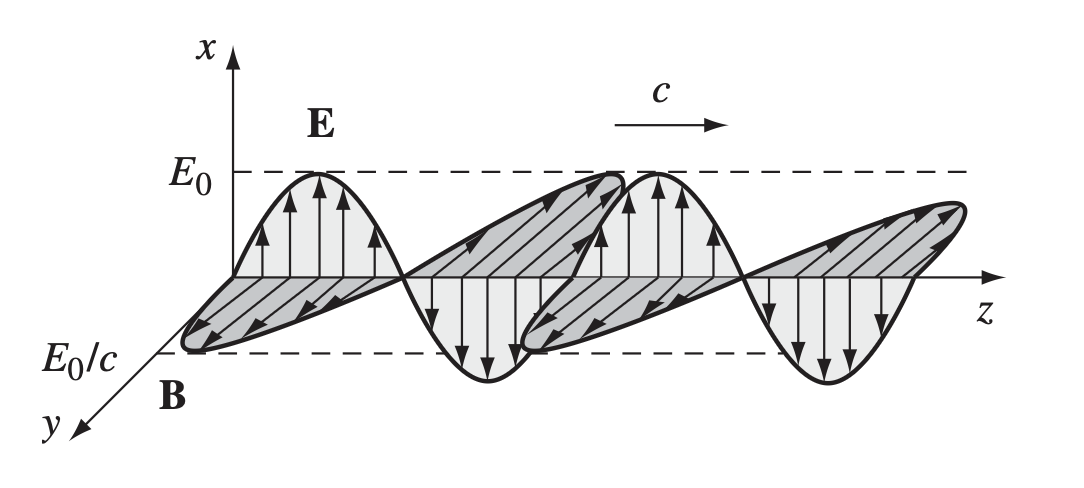
\includegraphics[width=0.8\textwidth]{figure/image66.png}
    \caption{Onda monocromatica}
    \label{fig:}
\end{figure}


Dalle relazione precedenti si ha 

\begin{tcolorbox}[colback=yellow!10!white, colframe=orange!70!black, boxrule=0.8pt]
\begin{equation}
    \mathbf{E}_0 \cdot \mathbf{k} = 0 \quad , \quad \mathbf{B}_0 \cdot \mathbf{k} = 0
\end{equation}
\end{tcolorbox}

\newpage

Inoltre conoscendo una delle due ampiezze complesse e la propagazione dell'onda è possibile ricavare anche l'altra ampiezza complessa.

\begin{tcolorbox}[colback=yellow!10!white, colframe=orange!70!black, boxrule=0.8pt]
\begin{align}
    \mathbf{E}_0 = c (\mathbf{B}_0 \times \mathbf{u}_n) \\
    \mathbf{B}_0 = \frac{1}{c} (\mathbf{u}_n \times \mathbf{E}_0)
\end{align}
\end{tcolorbox}

O analogamente, in termini di $\mathbf{k}$

\begin{tcolorbox}[colback=yellow!10!white, colframe=orange!70!black, boxrule=0.8pt]
\begin{align}
    \mathbf{E}_0 = \frac{\omega}{c^2} (\mathbf{B}_0 \times \mathbf{k}) \\
    \mathbf{B}_0 = \frac{1}{\omega} (\mathbf{k} \times \mathbf{E}_0)
\end{align}
\end{tcolorbox}

Chiaramente l’onda piana è di fatto un’astrazione matematica in quanto non esiste una sorgente fisica infinitamente estesa nello spazio che la possa produrre. Le sorgenti reali hanno un’estensione finita e questo che fa sì che la soluzione dell’equazione delle onde elettromagnetiche possa essere molto complicata.
Tuttavia, per quanto possano essere complessi, fronti d’onda non planari possono essere comunque localmente approssimati con il piano tangente.

\subsection{Polarizzazione delle onde elettromagnetiche monocromatiche}

\newpage

\subsection{Energia di un'onda elettromagnetica monocromatica}

Dalla \ref{eq: densità_totale_energia} sappiamo che l'energia per unità di volume di un campo elettromagnetico è 

\begin{equation}
    u = \frac{1}{2} \left(\varepsilon_0 E^2 + \frac{1}{\mu_0}B^2\right)
\end{equation}

Nel caso dell'onda monocromatica si ha 

\begin{equation}
    B^2 = \frac{1}{c^2} E^2 = \mu_0 \varepsilon_0 E^2
\end{equation}

quindi il campo elettrico e magnetico danno lo stesso contributo

\begin{tcolorbox}[colback=yellow!10!white, colframe=orange!70!black, boxrule=0.8pt]
\begin{equation}
    u = \varepsilon_0 E^2 = \varepsilon_0 E_0^2 \cos^2(kx - \omega t)
\end{equation}
\end{tcolorbox}

Il flusso di energia (per unità di area e di tempo) trasportato dal campo è dato dal vettore di Poynting \eqref{eq: vettore_Poynting}

\begin{equation}
    \mathbf{S} = \frac{1}{\mu_0} (\mathbf{E} \times \mathbf{B})
\end{equation}

Allora, per lo stesso motivo di prima

\begin{tcolorbox}[colback=yellow!10!white, colframe=orange!70!black, boxrule=0.8pt]
\begin{equation}
    \mathbf{S} = c \varepsilon_0 E_0^2 \cos^2(kx - \omega t) \ \mathbf{u}_n = c u \ \mathbf{u}_n
\end{equation}
\end{tcolorbox}

Si nota che $\mathbf{S}$ è la densità di energia moltiplicata per la velocità dell'onda, in accordo con il teorema di Poynting \eqref{eq: teorema_di_Poynting}.

Tipicamente, però, non siamo interessati al vettore di Poyting o alla densità di energia in ogni istante, ma al loro \emph{valor medio}. La media del coseno quadro lungo un periodo completo è $\frac{1}{2}$, quindi 

\begin{tcolorbox}[colback=yellow!10!white, colframe=orange!70!black, boxrule=0.8pt]
\begin{align}
    \langle u \rangle = \frac{1}{2}\varepsilon_0 E_0^2 \\
    \langle \mathbf{S} \rangle = \frac{1}{2} c \varepsilon_0 E_0^2 \ \mathbf{u}_n
\end{align}
\end{tcolorbox}

La potenza media per unità di area trasportata da un'onda elettromagnetica è chiamata intensità: \mkeyword{intesità}

\begin{tcolorbox}[colback=yellow!10!white, colframe=orange!70!black, boxrule=0.8pt]
\begin{equation}
    I \equiv \langle S \rangle = \frac{1}{2} c \varepsilon_0 E_0^2
\end{equation}
\end{tcolorbox}

\newpage

\section{Onde sferiche nel vuoto}

Un caso altrettanto semplice dal punto di vista analitico (quanto irrealistico dal punto di vista fisico), è rappresentato dall'onda sferica. \\


\begin{figure}[h]
  \centering
  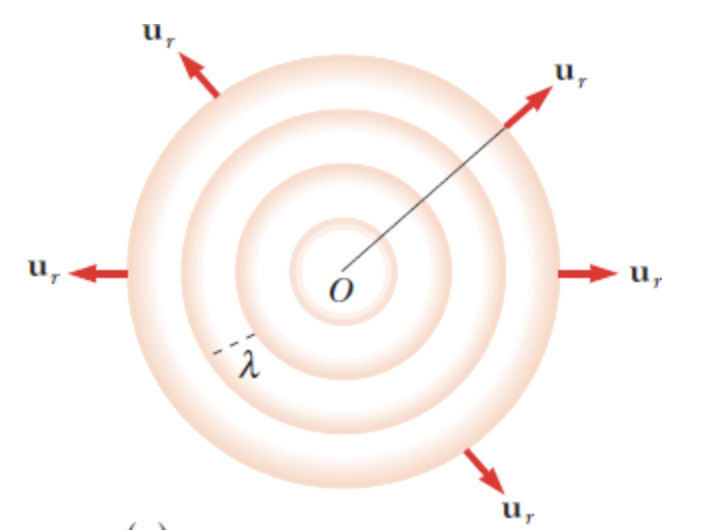
\includegraphics[width=0.4\linewidth]{figure/image67.png}
  \label{fig:etichetta}
\end{figure}

\'E opportuno, allora, tornare all'equazione generale delle onde scalari nello spazio tridimensionale 

\begin{equation}
    \nabla^2 \psi - \frac{1}{v^2} \frac{\partial^2 \psi}{\partial t^2}  
\end{equation}

dove la funzione d'onda dipende dalla posizione e dal tempo. 
Supponiamo che il problema abbia simmetria sferica, allora, tenendo conto dell'operato laplaciano in coordinate sferiche e della simmetria del problema, l'equazione precedente diventa

\begin{equation}
    \frac{1}{r} \frac{\partial^2 (r \psi)}{\partial r^2} = \frac{1}{v^2} \frac{\partial^2(\psi)}{\partial t^2}
\end{equation}

che è equivalente a 

\begin{equation}
    \frac{\partial^2 (r \psi)}{\partial r^2} = \frac{1}{v^2} \frac{\partial^2(r \psi)}{\partial t^2}
\end{equation}


Da un punto di vista strettamente matematico questa espressione è del tutto analoga all'equazione di d'Alembert per la funzione $r \psi$. Allora possiamo \emph{scegliere} come soluzione 

\begin{equation}
\psi(r,t) = \frac{A_{-} e^{i(kr - \omega t)}}{r} + \frac{A_{+} e^{i(kr + \omega t)}}{r}
\end{equation}

Limitando il nostro interesse ad onde armoniche esplosive, prodotte da una sorgente puntiforme con emissione isotropa (simmetria sferica) si ha che 

\begin{tcolorbox}[colback=yellow!10!white, colframe=orange!70!black, boxrule=0.8pt]
\begin{equation}
    \psi(r,t) = A \frac{e^{i(\mathbf{k}\cdot \mathbf{r} - \omega t)}}{r}
\end{equation}
\end{tcolorbox}

Poiché le equazioni di Maxwell nel vuoto, in assenza di sorgenti, si riducono a equazioni d'onda disaccoppiate per ciascuna componente dei campi $\mathbf{E}$ e $\mathbf{B}$, la soluzione trovata per $\psi$ può essere identificata con una qualsiasi componente cartesiana di questi campi. 
Tuttavia, non tutte le combinazioni sono fisicamente ammissibili: $\mathbf{E}$ e $\mathbf{B}$ devono soddisfare simultaneamente le equazioni di Maxwell, il che impone vincoli aggiuntivi - in particolare che i campi siano trasversali alla direzione di propagazione $\mathbf{u}_n$ e mutuamente ortogonali.

\newpage

\section{Onde cilindriche nel vuoto}

Un altro tipo di onde particolarmente importanti sono le onde cilindriche. \\

Tuttavia prima di trattare in dettaglio questo tipo di onde è necessario introdurre uno strumento matematico che ci servirà in seguito. 

\subsection{Funzioni di Bessel}

In coordinate cilindriche $(\rho, \phi, z)$ l'equazione di Laplace assume la forma 

\begin{equation}
    \frac{\partial^2 \psi}{\partial \rho^2} + \frac{1}{\rho} \frac{\partial \psi}{\partial \rho} + \frac{1}{\rho^2} \frac{\partial^2 \psi}{\partial \phi^2} + \frac{\partial^2 \psi}{\partial z^2} = 0
\end{equation}

La separazione delle variabili si ottiene con la sostituzione 

\begin{equation}
    \psi(\rho, \phi, z) = R(\rho) Q(\phi) Z(z)
\end{equation}

Questo conduce alle tre equazioni differenziali ordinarie:

\begin{align}
    \frac{d^2 Z}{dz^2} - k^2 Z = 0 \\
    \frac{d^2 Q}{d \phi^2} + \nu^2 Q = 0 \\
    \frac{d^2 R}{d \rho^2} + \frac{1}{\rho} \frac{dR}{d\rho} + \left( k^2 - \frac{\nu^2}{\rho^2} \right) R = 0
\end{align}

Le soluzioni alle prime due equazioni si ricavano facilmente:

\begin{align}
    Z(z) = e^{\pm kz}\\
    Q(\phi) = e^{\pm \nu \phi}
\end{align}

L'equazione radiale di può porre in una forma standard con il cambio di variabile $x = k\rho$. Essa diventa allora 

\begin{tcolorbox}[colback=yellow!10!white, colframe=orange!70!black, boxrule=0.8pt]
\begin{equation} \label{eq: equazione_Bessel}
    \frac{d^2 R}{dx^2} + \frac{1}{x} \frac{dR}{dx} + \left( 1 - \frac{\nu^2}{x^2} \right) R = 0
\end{equation}
\end{tcolorbox}

Questa è l'equazione di Bessel, \mkeyword{equazione di Bessel}e le sue soluzioni sono chiamate funzioni di Bessel di ordine $\nu$.\\

Se si assume un'equazione in serie di potenze del tipo 

\begin{equation}
    R(x) = x^{\alpha} \sum_{j = 0}^{\infty} a_j x^{j}
\end{equation}

sostituendo si ottiene che 

\begin{equation}
    \alpha = \pm \nu
\end{equation}

e 

\begin{equation}
    a_{2j} = - \frac{1}{4j (j + \alpha)} a_{2j-2}
\end{equation}

Tutte le potenze dispari di $x^j$ hanno coefficienti nulli. La formula di ricorrenza può essere iterata per dare 

\begin{equation}
a_{2 j}=\frac{(-1)^j \Gamma(\alpha+1)}{2^{2 j} j!\Gamma(j+\alpha+1)} a_0
\end{equation}

\'E conveniente porre la costante $a_0 = [2^\alpha \Gamma(\alpha +1)]^{-1}$. Le due soluzioni sono allora 

\begin{tcolorbox}[colback=yellow!10!white, colframe=orange!70!black, boxrule=0.8pt]
\begin{equation}
\begin{aligned}
J_\nu(x) & =\left(\frac{x}{2}\right)^\nu \sum_{j=0}^{\infty} \frac{(-1)^j}{j!\Gamma(j+\nu+1)}\left(\frac{x}{2}\right)^{2 j} \\
J_{-\nu}(x) & =\left(\frac{x}{2}\right)^{-\nu} \sum_{j=0}^{\infty} \frac{(-1)^j}{j!\Gamma(j-\nu+1)}\left(\frac{x}{2}\right)^{2 j}
\end{aligned}
\end{equation}
\end{tcolorbox}

Queste soluzioni sono chiamate funzioni di Bessel del primo tipo e di ordine $\pm \nu$. \mkeyword{funzioni di Bessel del primo tipo}

Se $\nu$ \emph{non} è intero, queste due soluzioni $J_{\pm \nu} (x)$ formano una coppia di soluzioni linearmente indipendenti. Tuttavia se $\nu$ è intero è ben noto che le soluzioni sono linearmente dipendenti. \\
In effetti, per $\nu = m$ intero, si può vedere dalla rappresentazione in serie che 

\begin{equation}
    J_{-m}(x) = (-1)^m J_m(x)
\end{equation}

Di conseguenza quando $\nu$ è intero è necessario trovare un'altra soluzione linearmente indipendente. Anche quando $\nu$ non è un intero è comune sostituire la coppia $j_{\pm}(x)$ con $J_{\nu}(x)$ e $N_{\nu} (x)$, quest'ultima è detta funzione di Neumann (o funzione di Bessel del secondo tipo) e vale: \mkeyword{funzione di Bessel del secondo tipo}

\begin{tcolorbox}[colback=yellow!10!white, colframe=orange!70!black, boxrule=0.8pt]
\begin{equation}
    N_{\nu} = \frac{J_{\nu}(x) \cos{\nu \pi} - J_{-\nu} (x)}{\sin{\nu \pi}}
\end{equation}
\end{tcolorbox}

Esistono anche le funzioni di Bessel del terzo\mkeyword{funzioni di Bessel del terzo tipo} tipo\footnote{per un approfondimento su questo argomento si consigli di guarda il capitolo 3.7 del \cite{ElettrodinamicaClassica}} che prendono il nome di funzioni di Hankel e sono le seguenti combinazioni lineari di $J_{\nu}(x)$ e $N_{\nu}(x)$:

\begin{tcolorbox}[colback=yellow!10!white, colframe=orange!70!black, boxrule=0.8pt]
\begin{equation}
\begin{array}{l}
H_\nu^{(1)}(x)=J_\nu(x)+i N_\nu(x) \\
H_\nu^{(2)}(x)=J_\nu(x)-i N_\nu(x)
\end{array}
\end{equation}
\end{tcolorbox}

\newpage

Particolarmente interessanti sono le forme asintotiche delle funzioni di Bessel per valori molto grandi e molto piccolo dei loro argomenti. \\

Se supponiamo $x \ll 1$:

\begin{tcolorbox}[colback=yellow!10!white, colframe=orange!70!black, boxrule=0.8pt]
\begin{align}
J_{\nu}(x) \rightarrow \frac{1}{\Gamma(\nu+1)}\left(\frac{x}{2}\right)^{\nu}\\
N_{\nu}(x) \rightarrow
\begin{cases}
  \dfrac{2}{\pi}\left[\ln\left(\frac{x}{2}\right) + 0{,}5772\cdots\right], & \nu = 0 \\[10pt]
  -\dfrac{\Gamma(\nu)}{\pi}\left(\frac{2}{x}\right)^{\nu}, & \nu \neq 0
\end{cases}
\end{align}
\end{tcolorbox}

Se supponiamo $x \gg 1$:

\begin{tcolorbox}[colback=yellow!10!white, colframe=orange!70!black, boxrule=0.8pt]
\begin{align}
    J_{\nu}(x) \rightarrow \sqrt{\frac{2}{\pi x}}\cos\left(x - \frac{\nu\pi}{2} - \frac{\pi}{4}\right)\\
    N_{\nu}(x) \rightarrow \sqrt{\frac{2}{\pi x}}\sin\left(x - \frac{\nu\pi}{2} - \frac{\pi}{4}\right)
\end{align}
\end{tcolorbox}

Adesso possiamo passare alla formulazione formale delle onde cilindriche.\\

\begin{figure}[h]
  \centering
  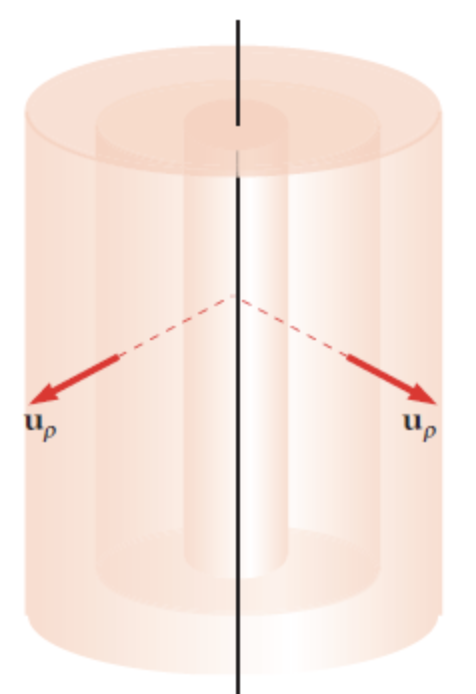
\includegraphics[width=0.3\linewidth]{figure/image68.png}
  \caption{Onda cilindrica}
  \label{fig:etichetta}
\end{figure}

Per descriverle conviene usare un sistema di coordinate cilindriche con l'asse $z$ coincidente con la retta sorgente. Supponendo che le coordinate del campo elettrico e magnetico dipendano solo da $\rho$, per ciascuna componente dei campi vale 

\begin{equation}
    \frac{1}{\rho} \frac{\partial \psi}{\partial \rho} + \frac{\partial^2 \psi}{\partial \rho^2} = \frac{1}{v^2} \frac{\partial^2 \psi}{\partial t^2}
\end{equation}

Procedendo per separazione delle variabili, ed assumendo dipendenza temporale armonica semplice, si pone 

\begin{equation}
    \psi(\rho,t) = R(\rho) e^{-i \omega t}
\end{equation}

in cui la parte spaziale $R(\rho)$ deve essere soluzione di 

\begin{equation}
    \rho \frac{d^2 R}{d \rho^2} + \frac{dR}{d\rho} - k^2 \rho R = 0
\end{equation}

La quale è la funzione di Bessel \eqref{eq: equazione_Bessel} dove $x = k\rho$ e si ha che $\nu = 0$. Pertanto, dato che siamo nel caso in cui $\nu$ è intero, si ha che la soluzione è 

\begin{equation}
        R(\rho) = A J_{0}(k\rho) + B N_{0} (k\rho)
\end{equation}

Dove $A$ e $B$ sono due costanti di integrazione. \\

Se supponiamo di essere nel caso $k \rho \gg 1$ si ha che 

\begin{tcolorbox}[colback=yellow!10!white, colframe=orange!70!black, boxrule=0.8pt]
\begin{equation}
    J_0(k \rho) \approx \sqrt{\frac{2}{\pi k \rho}} \cos \left(k \rho - \frac{\pi}{4}\right) \quad , \quad N_{0}(k \rho) \approx \sqrt{\frac{2}{\pi k \rho}} \sin\left(k \rho - \frac{\pi}{4}\right)
\end{equation}
\end{tcolorbox}

Quindi, in questo limite 

\begin{tcolorbox}[colback=yellow!10!white, colframe=orange!70!black, boxrule=0.8pt]
\begin{equation}
\psi (\rho, t) = \frac{A_p}{\sqrt{\rho}} e^{i(k\rho - \omega t)} + \frac{A_r}{\sqrt{\rho}} e^{i(k \rho + \omega t)}
\end{equation}
\end{tcolorbox}

La parte della soluzione con $J_0$ è legata ad onde convergenti, quella con $N_0$ alle onde divergenti. Quanto detto vale per onde scalari, che si propagano nella direzione del versore $\mathbf{u}_{\rho}$

\newpage

\section{Onde elettromagnetiche in assenza di sorgenti in un mezzo}

Supponiamo di essere in un mezzo, ma in una regione in cui non siano presenti cariche libere e correnti di conduzione, per cui $\rho = 0$ e $\mathbf{j} = 0$. 

In queste ipotesi le equazioni di Maxwell possono essere scritte come 

\begin{align*}
    \nabla \cdot \mathbf{D} = 0 \\
    \nabla \cdot \mathbf{B} = 0 \\
    \nabla \times \mathbf{E} = -\dfrac{\partial \mathbf{B}}{\partial t} \\
    \nabla \times \mathbf{H} = \dfrac{\partial \mathbf{D}}{\partial t}
\end{align*}

Se il mezzo è lineare:

\begin{equation}
    \mathbf{D} = \varepsilon \mathbf{E} \quad , \quad \mathbf{H} = \frac{1}{\mu} \mathbf{B}
\end{equation}

e omogeneo (in modo che $\eps$ e $\mu$ non varino nello spazio), le equazioni si riducono a 

\begin{align*}
    \nabla \cdot \mathbf{E} = 0 \\
    \nabla \cdot \mathbf{B} = 0 \\
    \nabla \times \mathbf{E} = -\dfrac{\partial \mathbf{B}}{\partial t} \\
    \nabla \times \mathbf{B} = \mu \varepsilon \dfrac{\partial \mathbf{E}}{\partial t}
\end{align*}

che differiscono con l'analogo corrispondente nel vuoto solo per il termine $\eps \mu$. \\

\emph{Pertanto tutti i risultati ottenuti in precedenza sono ancora validi, cambia solamente che al posto di $c$ dobbiamo mettere $v$, dove}

\begin{tcolorbox}[colback=yellow!10!white, colframe=orange!70!black, boxrule=0.8pt]
\begin{equation}
    v = \frac{1}{\sqrt{\eps \mu}} = \frac{c}{n} 
\end{equation}
\end{tcolorbox}

dove 

\begin{tcolorbox}[colback=yellow!10!white, colframe=orange!70!black, boxrule=0.8pt]
\begin{equation}
    n = \sqrt{\frac{\eps \mu}{\eps_0 \mu_0}}
\end{equation}
\end{tcolorbox}

è l'indice di rifrazione della sostanza. \mkeyword{indice di rifrazione}Per la maggior parte dei materiali, il valore di $\mu$ è molto vicino a quello di $\mu_0$, quindi

\begin{equation}
    n \approx\sqrt{\kappa_e}
\end{equation}

\subsection{Onde monocromatiche in un mezzo}

Anche i risultati per le onde monocromatiche continuano a essere validi, è però interessante vedere come cambia la densità di energia e il vettore di Poynting. \\

La densità di energia risulta essere 

\begin{equation}
    u = \frac{1}{2} \left( \eps E^2 + \frac{1}{\mu} B^2 \right)
\end{equation}

e il vettore di Poynting è 

\begin{equation}
    \mathbf{S} = \frac{1}{\mu} (\mathbf{E} \times \mathbf{B})
\end{equation}

In particolare, per le onde monocromatiche piane, per quanto visto prima, vale 

\begin{tcolorbox}[colback=yellow!10!white, colframe=orange!70!black, boxrule=0.8pt]
\begin{equation}
    I = \frac{1}{2} \eps v E_0^2 = \frac{1}{2} \frac{n}{Z_0} E_0^2
\end{equation}
\end{tcolorbox}

dove abbiamo posto 

\begin{tcolorbox}[colback=yellow!10!white, colframe=orange!70!black, boxrule=0.8pt]
\begin{equation}
    Z_0 = \sqrt{\frac{\mu_0}{\eps_0}} \approx 377 \Omega
\end{equation}
\end{tcolorbox}

Questa quantità prende il nome di impedenza nel vuoto. \mkeyword{impedenza nel vuoto}

\newpage

\section{Soluzione equazione d'onda con sorgente}

Consideriamo adesso il caso generale delle equazioni di Maxwell, cioè il caso in cui siano presenti anche delle sorgenti.\\

Osservando le equazioni di Maxwell in forma potenziale in gauge di Lorenz \ref{eq: Gauge_Lorenz}, si nota che le equazioni sono tutte nella stessa forma, cioè

\begin{tcolorbox}[colback=yellow!10!white, colframe=orange!70!black, boxrule=0.8pt]
\begin{equation}\label{eq: equazione_onda_non_omogenea}
    \nabla^2 \psi - \frac{1}{c^2} \frac{\partial^2 \psi}{\partial t^2} = -4 \pi f(\mathbf{r},t)
\end{equation}
\end{tcolorbox}

Dove il termine $-4 \pi$ è stato aggiunto per un motivo che sarà chiaro tra poco. \\

Andiamo a trovare una soluzione generale a questa equazione.\\

Possiamo considerare una generica sorgente $f(\mathbf{r}, t)$ come una sovrapposizione di sorgenti puntiformi

\begin{equation}
    f(\mathbf{r}, t) = \int \int f(\mathbf{r'}, t') \delta(\mathbf{r} - \mathbf{r'}) \delta(t - t') d^3 r' dt'
\end{equation}

ma allora si intuisce che $\psi$ dovrà essere nella forma 

\begin{equation}
    \psi (\mathbf{r}, t) = \int \int G(\mathbf{r},\mathbf{r'}, t, t') f (\mathbf{r'}, t') d^3 r' dt'
\end{equation}

Dove $G(\mathbf{r},\mathbf{r'}, t, t')$ è la funzione di Green associata all'operatore dalembertiano, cioè la funzione che soddisfa la relazione 

\begin{equation}
    \Box^2 G(\mathbf{r}, \mathbf{r'}, t, t') = - 4 \pi \delta(\mathbf{r} - \mathbf{r'}) \delta(t -t')
\end{equation}

Pertanto, sostituendo, la \ref{eq: equazione_onda_non_omogenea} si riduce a 

\begin{tcolorbox}[colback=yellow!10!white, colframe=orange!70!black, boxrule=0.8pt]
\begin{equation} \label{eq: equazione_onda_non_omogena_Green}
    (\nabla^2 - \frac{1}{c^2} \partial_t^2) G(\mathbf{r}, \mathbf{r'}, t, t') = -4 \pi \delta(\mathbf{r} - \mathbf{r'})\delta (t - t') 
\end{equation}
\end{tcolorbox}

Inoltre sappiamo che possiamo esprimere la delta secondo la trasformata di Fourier come 

\begin{equation}
    \delta(t - t') = \frac{1}{2\pi} \int_{-\infty}^{\infty} e^{-i \omega (t-t')} d\omega
\end{equation}

Poiché la sorgente è una sovrapposizione di termini $e^{-i\omega t}$, per linearità dell'equazione cerchiamo $G(\mathbf{r}, \mathbf{r'}, t, t')$ della stessa forma:

\begin{tcolorbox}[colback=yellow!10!white, colframe=orange!70!black, boxrule=0.8pt]
\begin{equation} \label{eq: legame_Green_tempo_spazio}
    G(\mathbf{r}, \mathbf{r'}, t, t') = \frac{1}{2\pi} \int_{-\infty}^{\infty} \tilde{G}_{\omega}(\mathbf{r}, \mathbf{r'}) \cdot e^{-i \omega (t -t')} d\omega
\end{equation}
\end{tcolorbox}

Dove $\tilde{G}_{\omega}$ rappresenta la parte spaziale da determinare. 

\newpage

Applicando il dalembertiano al nostro ansatz si ha:

\begin{align}
    \nabla^2 G = \frac{1}{2\pi} \int_{-\infty} \nabla^2 \tilde{G}_{\omega} \cdot e^{-i \omega (t-t')} d\omega\\
    -\frac{1}{c^2} \frac{\partial^2}{\partial t^2} G = \frac{1}{2\pi} \int_{-\infty}^{\infty} \frac{\omega^2}{c^2} \tilde{G}_{\omega} \cdot e^{-i \omega (t - t')} d \omega
\end{align}

Allora raccogliendo tutto la \ref{eq: equazione_onda_non_omogena_Green} diventa 

\begin{equation}
\frac{1}{2\pi} \int_{-\infty}^{\infty} \left( \nabla^2 + \frac{\omega^2}{c^2} \right) \tilde{G}_{\omega} \cdot e^{-i\omega (t-t')} d\omega = \frac{1}{2\pi} \int_{-\infty}^{\infty} \left( -4\pi \delta(\mathbf{r} - \mathbf{r'}) \right) \cdot e^{-i\omega (t-t')} d\omega
\end{equation}

Poiché questo deve valere per ogni $\omega$, i termini sotto l'integrale devono essere uguali frequenza per frequenza:

\begin{tcolorbox}[colback=yellow!10!white, colframe=orange!70!black, boxrule=0.8pt]
\begin{equation}\label{eq: equazione_Helmholtz}
    \left( \nabla^2 + \frac{\omega^2}{c^2} \right) \tilde{G}_{\omega} = - 4\pi \delta(\mathbf{r} - \mathbf{r'})
\end{equation}
\end{tcolorbox}

Ci siamo quindi ricondotti a un nuovo tipo di equazione che prende il nome di equazione di Helmholtz. \mkeyword{equazione di Helmholtz}

\subsection{Soluzione equazione di Helmholtz}

Poniamo $k = \frac{\omega}{c}$, allora la \ref{eq: equazione_Helmholtz} diventa

\begin{equation}
    (\nabla^2 + k^2) \tilde{G}_{\omega} (\mathbf{r}, \mathbf{r'}) = -4\pi \delta(\mathbf{r} - \mathbf{r'})
\end{equation}

Allora si nota che $\tilde{G}_{\omega}$ non è altro che la funzione di Green associata all'operatore $(\nabla^2 + k^2)$.\\

Se non vi sono superfici di confine, la funzione di Green può dipendere soltanto da $\mathbf{R} = \mathbf{r} - \mathbf{r'}$, e deve essere a simmetria sferica, ossia deve dipendere soltato da $R = |\mathbf{R}|$. Dalla forma dell'operatore laplaciano in coordinate sferiche è chiaro che $\tilde{G}_{\omega}(R)$ soddisfa 

\begin{equation}
    \frac{1}{R}\frac{d^2}{dR^2} (R \tilde{G}_{\omega}) + k^2 \tilde{G}_{\omega} = -4 \pi\delta(R) 
\end{equation}

Dato che stiamo considerano un'equazione con una delta, $R \tilde{G}_{\omega}(R)$ soddisfa in tutto lo spazio tranne che in $R = 0$ l'equazione omogenea 

\begin{equation}
    \frac{d^2}{dR^2} (R \tilde{G}_{\omega}) + k^2 (R \tilde{G}_{\omega}) = 0
\end{equation}

con soluzione 

\begin{equation}
    R \tilde{G}_{\omega}(R) = A e^{ikR} + B e^{-ikR}
\end{equation}

Mentre quando $R \to 0$ siamo vicini alla sorgente puntuale e in questo limite $kR \ll 1$, il che significa che il termine $k^2$ nell'equazione di Helmholtz diventa trascurabile rispetto a $\nabla^2$, e l'equazione si riduce a quella di Poisson:

\begin{equation}
    \nabla^2 \tilde{G}_{\omega} \approx -4\pi \delta(R)
\end{equation}

Dall'equazione di Poisson sappiamo già che la soluzione è il potenziale columbiano: 

\begin{equation}
    \tilde{G}_{\omega}(R) \xrightarrow{R \to 0} \frac{1}{R}
\end{equation}

Questo fissa la normalizzazione. Guardando la soluzione generale:

\begin{equation*}
    R \tilde{G}_{\omega}(R) = A e^{ikR} + B e^{-ikR}
\end{equation*}

Per $R \to 0$ si ha che $e^{\pm i kR} \to 1$, quindi:

\begin{equation*}
    R \tilde{G}_{\omega}(R) \to A + B \implies \tilde{G}_{\omega}(R) \xrightarrow{R \to 0} \frac{A + B}{R}
\end{equation*}

Affinché questo coincida con $1/R$, bisogna imporra:

\begin{equation}
    A + B = 1
\end{equation}

Questo è il vincolo che fissa la normalizzazione della soluzione generale. \\

Pertanto si ha che la soluzione generale dell'equazione di Helmholtz è 

\begin{tcolorbox}[colback=yellow!10!white, colframe=orange!70!black, boxrule=0.8pt]
\begin{align} 
    \tilde{G}_{\omega}(R) = A \tilde{G}_{\omega}^{(+)}(R) + B \tilde{G}_{\omega}^{(-)}(R) \\
    A + B = 1
\end{align}
\end{tcolorbox}

Dove abbiamo definito 

\begin{tcolorbox}[colback=yellow!10!white, colframe=orange!70!black, boxrule=0.8pt]
\begin{align} 
    \tilde{G}_{\omega}^{(\pm)}(R) = \frac{e^{\pm i k R}}{R} 
\end{align}
\end{tcolorbox}

Allora possiamo andare a sostituire questo risultato nella \ref{eq: legame_Green_tempo_spazio} e ottenere

\begin{equation}
    G^{(\pm)} (R, \tau) = \frac{1}{2\pi} \int_{-\infty}^{+\infty} \frac{e^{\pm ikR}}{R} \cdot e^{-i\omega \tau} \ d\omega
\end{equation}

Dove abbiamo posto $\tau = t - t'$. Si nota che questo integrale è una delta e quindi le funzioni di Green sono 

\begin{equation}
    G^{(\pm)}(R, \tau) = \frac{1}{R} \delta(\tau \mp \frac{R}{c}) 
\end{equation}

oppure, più esplicitamente

\begin{tcolorbox}[colback=yellow!10!white, colframe=orange!70!black, boxrule=0.8pt]
\begin{equation}
    G^{(\pm)}(\mathbf{r}, \mathbf{r'}, t, t') = \frac{\delta \left(t' - \left[ t \mp \frac{|\mathbf{r} - \mathbf{r}'|}{c} \right] \right)}{|\mathbf{r} - \mathbf{r'}|}
\end{equation}
\end{tcolorbox}

La funzione di Green $G^{(+)}$ è chiamata \emph{funzione di Green ritardata} \mkeyword{funzione di Green ritardata} perché esibisce il comportamento causale associato ad una perturbazione ondulatoria.
L'argomento della funziona delta mostra che un effetto osservato nel punto $\mathbf{r}$ all'istante $t$ è causato dall'azione di una sorgente a distanza $R$ in un istante precendete o ritardato $t' = t - R/c$. La differenza temporale $R/c$ è semplicemente il tempo di propagazione della perturbazione da un punto all'altro. \\

Analogamente, $G^{(-)}$ è chiamata \emph{funzione di Green anticipata}. \mkeyword{funzione di Green anticipata}\\

Gli integrali particolari dell'equazione d'onda non omogenea sono

\begin{equation}
    \psi^{(\pm)}(\mathbf{r}, t) = \int \int G^{(\pm)}(\mathbf{r}, \mathbf{r'}, t, t') f(\mathbf{r'}, t') \, d^3r' \, dt'
\end{equation}

Per determinare un problema fisico assegnato, può essere necessario aggiungere ad entrambe queste soluzioni una soluzione dell'equazione omogenea. Consideriamo una distribuzione di sorgenti $f(\mathbf{r'}, t')$ che sia localizzata nello spazio e nel tempo. Essa è diversa da zero solo per un intervallo temporale limitato attorno a $t' = 0$. Si possono identificare due situazioni limite. \\

Nella prima si assume che per $t \to -\infty$ vi sia un'onda $\psi_{\text{in}}$ che soddisfa l'equazione d'onda omogenea. Questa onda si propaga nel tempo e nello spazio; la sorgente si accende e genera le sue proprie onde. La soluzione completa a tutti i tempi per questa situazione è chiaramente

\begin{equation}
    \psi(\mathbf{r}, t) = \psi_{\text{in}}(\mathbf{r}, t) + \int \int G^{(+)}(\mathbf{r}, \mathbf{r'}, t, t') f(\mathbf{r'}, t') \, d^3r' \, dt'
\end{equation}

La presenza di $G^{(+)}$ assicura che nel lontano passato, prima che la sorgente venga attivata, non vi sono contributi all'integrale. È presente soltanto l'onda assegnata $\psi_{\text{in}}$. \\

La seconda situazione è quella per cui a tempi lontani nel futuro ($t \to +\infty$) venga assegnata l'onda $\psi_{\text{out}}$, una soluzione nota dell'equazione d'onda omogenea. La soluzione completa a tutti i tempi è allora

\begin{equation}
    \psi(\mathbf{r}, t) = \psi_{\text{out}}(\mathbf{r}, t) + \int \int G^{(-)}(\mathbf{r}, \mathbf{r'}, t, t') f(\mathbf{r'}, t') \, d^3r' \, dt'
\end{equation}

La funzione di Green anticipata garantisce ora l'assenza di qualsiasi segnale dalla sorgente una volta che questa sia stata spenta (tali segnali sono per definizione contenuti in $\psi_{\text{out}}$). \\

La situazione fisica più comune è descritta dall'equazione precedente con $\psi_{\text{in}} = 0$. Essa viene a volte scritta sostituendo esplicitamente la funzione di Green:

\begin{tcolorbox}[colback=yellow!10!white, colframe=orange!70!black, boxrule=0.8pt]
\begin{equation} \label{eq: soluzioni_ritardate}
    \psi(\mathbf{r}, t) = \int \frac{\left[ f(\mathbf{r'}, t') \right]_{\text{rit}}}{|\mathbf{r} - \mathbf{r'}|} \, d^3r'
\end{equation}
\end{tcolorbox}

La parentesi quadra $[\cdots]_{\text{rit}}$ significa che il tempo $t'$ deve essere calcolato all'istante ritardato $t' = t - |\mathbf{r} - \mathbf{r'}|/c$.

\section{Potenziali ritardati}

Utilizzando le soluzioni ritardate \ref{eq: soluzioni_ritardate} per le equazioni d'onda \ref{eq: Gauge_Lorenz} si ottiene 

\begin{tcolorbox}[colback=yellow!10!white, colframe=orange!70!black, boxrule=0.8pt]
\begin{align} \label{potenziali ritardati}
    \phi(\mathbf{r},t) = \frac{1}{4\pi \eps_0} \int_{\tau} \frac{[\rho (\mathbf{r'}, t')]_{\text{rit}}}{|\mathbf{r} - \mathbf{r'}|} d^3r' = \frac{1}{4\pi \eps_0} \int_{\tau} \frac{\rho (\mathbf{r'}, t - \frac{|\mathbf{r} - \mathbf{r}'|}{c})}{|\mathbf{r} - \mathbf{r'}|} d^3r'\\
    \mathbf{A}(\mathbf{r},t) = \frac{\mu_0}{4\pi} \int_{\tau} \frac{[\mathbf{j}(\mathbf{r}', t')]_{\text{rit}}}{|\mathbf{r} - \mathbf{r'}|} d^3 r' = \frac{\mu_0}{4\pi} \int_{\tau} \frac{\mathbf{j}(\mathbf{r}', t - \frac{|\mathbf{r} - \mathbf{r}'|}{c})}{|\mathbf{r} - \mathbf{r'}|} d^3 r' 
\end{align}
\end{tcolorbox}

I potenziali ritardati \ref{potenziali ritardati} sono la generalizzazione dinamica dei potenziali statici di Coulomb e Biot-Savart: la distribuzione di carica e corrente che contribuisce al potenziale nel punto $\mathbf{r}$ all'istante $t$ non è quella presente in $\mathbf{r'}$ all'istante $t$, bensì quella presente all'istante ritardato $t' = t - |\mathbf{r} - \mathbf{r'}|/c$, cioè il tempo necessario affinché un segnale che viaggia alla velocità della luce raggiunga $\mathbf{r}$ da $\mathbf{r'}$.\\

Questo risultato è fisicamente fondamentale: i campi elettromagnetici non si propagano istantaneamente, ma con velocità $c$, in accordo con la causalità relativistica. \footnote{\'E possibile ottenere anche un'espressione esplicita per i campi grazie all'equazione di Jefimenko, tuttavia l'utilità di questi è limitata dato che solitamente è più semplice calcolare i potenziali ritardati e differenziarli se necessario. 
Si trovano approfondimenti in \cite{ElettrodinamicaClassica} e \cite{IntroductiontoElectrodynamics}}

\subsection{Potenziali di Liénard-Wiechert}

Un caso particolarmente importante e istruttivo è quello di una carica puntiforme $q$ in moto con traiettoria $\mathbf{r}_q(t)$ e velocità  $\mathbf{v}(t) = \dot{\mathbf{r}}_q(t)$. Le distribuzioni di carica e corrente sono:

\begin{align}
    \rho(\mathbf{r'}, t') = q \, \delta(\mathbf{r'} - \mathbf{r}_q(t')) \\
    \mathbf{j}(\mathbf{r'}, t') = q \, \mathbf{v}(t') \delta(\mathbf{r'} - \mathbf{r}_q(t'))
\end{align}

Sostituendo nelle \ref{potenziali ritardati} e integrando con attenzione — tenendo conto che la delta temporale introduce un fattore geometrico dovuto alla dipendenza di $|\mathbf{r} - \mathbf{r'}|$ dalla posizione della carica — si ottengono i \emph{potenziali di Liénard-Wiechert}: \mkeyword{potenziali di Liénard-Wiechert}

\begin{tcolorbox}[colback=yellow!10!white, colframe=orange!70!black, boxrule=0.8pt]
\begin{align} \label{eq: potenziali_Liènard-Wiechert}
    \phi(\mathbf{r}, t) = \frac{q}{4\pi\varepsilon_0} \left( \frac{1}{\mathcal{R} - \boldsymbol{\mathcal{R}} \cdot \boldsymbol{\beta}} \right)_{\text{rit}} \\
    \mathbf{A}(\mathbf{r}, t) = \frac{\mu_0 q c}{4\pi} \left( \frac{\boldsymbol{\beta}}{\mathcal{R} - \boldsymbol{\mathcal{R}} \cdot \boldsymbol{\beta}} \right)_{\text{rit}}
\end{align}
\end{tcolorbox}

dove abbiamo definito:

\begin{align}
    \boldsymbol{\mathcal{R}} = \mathbf{r} - \mathbf{r}_q(t') \quad &, \quad \mathcal{R} = |\boldsymbol{\mathcal{R}}| \\
    \boldsymbol{\beta} = \frac{\mathbf{v}(t')}{c} \quad &, \quad \beta = |\boldsymbol{\beta}|
\end{align}

tutti valutati all'istante ritardato $t'$. Il fattore $(1 - \hat{\mathcal{R}} \cdot \boldsymbol{\beta})$ al denominatore è una conseguenza geometrica della propagazione finita del segnale: una carica che si avvicina all'osservatore con velocità prossima a $c$ produce un campo molto più intenso rispetto al caso statico, mentre una carica che si allontana lo produce più debole — un effetto analogo all'effetto Doppler relativistico.

Si noti inoltre la relazione semplice tra i due potenziali:

\begin{tcolorbox}[colback=yellow!10!white, colframe=orange!70!black, 
boxrule=0.8pt]
\begin{equation}
    \mathbf{A}(\mathbf{r}, t) = \frac{\boldsymbol{\beta}_{\text{rit}}}{c} 
    \phi(\mathbf{r}, t)
\end{equation}
\end{tcolorbox}

\section{Sorgenti monocromatiche e sviluppo in multipoli}

Consideriamo sorgenti con dipendenza temporale armonica, ovvero 

\begin{equation}
    \rho(\mathbf{r'}, t) = \rho(\mathbf{r'}) e^{-i\omega t} \quad , \quad 
    \mathbf{j}(\mathbf{r'}, t) = \mathbf{j}(\mathbf{r'}) e^{-i\omega t}
\end{equation}

Per linearità delle equazioni, anche i potenziali avranno la stessa dipendenza temporale:

\begin{equation}
    \phi(\mathbf{r}, t) = \phi(\mathbf{r}) e^{-i\omega t} \quad , \quad 
    \mathbf{A}(\mathbf{r}, t) = \mathbf{A}(\mathbf{r}) e^{-i\omega t}
\end{equation}

Sostituendo nei potenziali ritardati \ref{potenziali ritardati}, il tempo ritardato $t_r = t - |\mathbf{r} - \mathbf{r'}|/c$ introduce un fattore di fase $e^{ik|\mathbf{r}-\mathbf{r'}|}$, con $k = \omega/c$, e le parti spaziali dei potenziali diventano:

\begin{tcolorbox}[colback=yellow!10!white, colframe=orange!70!black, 
boxrule=0.8pt]
\begin{align}
    \phi(\mathbf{r}) = \frac{1}{4\pi\varepsilon_0} \int 
    \rho(\mathbf{r'}) \frac{e^{ik|\mathbf{r}-\mathbf{r'}|}}
    {|\mathbf{r}-\mathbf{r'}|} \, d^3r' \\[6pt]
    \mathbf{A}(\mathbf{r}) = \frac{\mu_0}{4\pi} \int 
    \mathbf{j}(\mathbf{r'}) \frac{e^{ik|\mathbf{r}-\mathbf{r'}|}}
    {|\mathbf{r}-\mathbf{r'}|} \, d^3r'
\end{align}
\end{tcolorbox}

Il nucleo comune a entrambi gli integrali è la funzione di Green dell'operatore di Helmholtz:

\begin{equation}
    G(\mathbf{r}, \mathbf{r'}) = \frac{e^{ik|\mathbf{r}-\mathbf{r'}|}}
    {|\mathbf{r}-\mathbf{r'}|}
\end{equation}

Supponiamo ora che la sorgente sia confinata in un volume di dimensione tipica $d$, e cerchiamo i campi a distanza $r = |\mathbf{r}| \gg d$. 
In questa ipotesi è possibile espandere $G$ in potenze di $r'/r \ll 1$.\\

Partendo dall'identità geometrica esatta

\begin{equation}
    |\mathbf{r} - \mathbf{r'}| = r\sqrt{1 - 2\frac{\hat{r}\cdot\mathbf{r'}}{r} 
    + \frac{r'^2}{r^2}} \approx r - \hat{r}\cdot\mathbf{r'}
\end{equation}

\newpage

valida al primo ordine in $r'/r$, si ottiene:

\begin{equation}
    G(\mathbf{r}, \mathbf{r'}) \approx \frac{e^{ikr}}{r} \, 
    e^{-ik\hat{r}\cdot\mathbf{r'}}
\end{equation}

dove abbiamo approssimato $1/|\mathbf{r}-\mathbf{r'}| \approx 1/r$ nell'ampiezza (lecito per $r \gg d$) ma mantenuto la correzione $e^{-ik\hat{r}\cdot\mathbf{r'}}$ nella fase, poiché anche piccole variazioni di fase possono avere effetti significativi.\\

Espandendo infine l'esponenziale in serie:

\begin{tcolorbox}[colback=yellow!10!white, colframe=orange!70!black, boxrule=0.8pt]
\begin{equation} \label{eq: sviluppo_multipoli_ritard}
    e^{-ik\hat{r}\cdot\mathbf{r'}} = \sum_{n=0}^{\infty} 
    \frac{(-ik)^n}{n!} (\hat{r}\cdot\mathbf{r'})^n 
    = 1 - ik(\hat{r}\cdot\mathbf{r'}) + \cdots
\end{equation}
\end{tcolorbox}

Il primo termine ($n=0$) corrisponde all'approssimazione di dipolo elettrico, in cui il tempo ritardato è lo stesso per tutta la sorgente e non dipende da $\mathbf{r'}$. In altre parole, questa è l'approssimazione in cui stiamo considerando la sorgente come un oggetto puntiforme che oscilla come un unico dipolo.

\subsection{Le tre zone}

Prima di procedere con il calcolo esplicito dei campi, è utile identificare tre regioni dello spazio con caratteristiche fisiche distinte, determinate dal confronto tra $r$, $d$ e la lunghezza d'onda $\lambda = 2\pi/k$:

\begin{itemize}
    \item \textbf{Zona quasi-statica} (campo prossimo): $d \ll r \ll \lambda$, 
    ovvero $kr \ll 1$. In questo regime $e^{ikr}/r \approx 1/r$ e i campi 
    hanno la stessa struttura dei campi statici, con una dipendenza 
    temporale $e^{-i\omega t}$.

    \item \textbf{Zona di induzione} (campo intermedio): $d \ll r \sim \lambda$, 
    ovvero $kr \sim 1$. I termini di velocità e di accelerazione sono 
    comparabili, e la struttura dei campi è più complicata. Questa zona 
    è rilevante per esempio nelle antenne in campo vicino.

    \item \textbf{Zona di radiazione} (campo lontano): $d \ll \lambda \ll r$, 
    ovvero $kr \gg 1$. Dominano i termini che decadono come $1/r$, 
    responsabili del trasporto netto di energia. Questa è la zona 
    fisicamente più importante per lo studio dell'irraggiamento.
\end{itemize}

\newpage

\section{Dipolo elettrico oscillante}

Consideriamo una distribuzione di cariche e correnti monocromatica confinata in un volume piccolo ($d \ll \lambda$). Nell'approssimazione di dipolo \emph{elettrico} ($n=0$ nello sviluppo precedente) il potenziale vettore è:

\begin{equation}
    \mathbf{A}_0(\mathbf{r}) = \frac{\mu_0}{4\pi} \frac{e^{ikr}}{r} 
    \int \mathbf{j}(\mathbf{r'}) \, d^3r'
\end{equation}

L'integrale della densità di corrente è collegato alla derivata temporale del momento di dipolo elettrico. Utilizzando l'equazione di continuità $\nabla \cdot \mathbf{j} = -\partial_t \rho = i\omega\rho$ e integrando per parti, si dimostra che:

\begin{equation}
    \int \mathbf{j}(\mathbf{r'}) \, d^3r' = -\int \mathbf{r}' (\nabla' \cdot \mathbf{j}) = -i\omega \int \mathbf{r}' \rho(\mathbf{r}') \ d^3 r' = -i\omega \mathbf{p}_0
\end{equation}

dove $\mathbf{p}_0 = \int \rho(\mathbf{r'}) \mathbf{r'} \, d^3r'$ è l'ampiezza del momento di dipolo elettrico. Definendo il momento di dipolo come $\mathbf{p}(t) = \mathbf{p}_0 e^{-i\omega t}$ e al tempo ritardato $\mathbf{p}_r = \mathbf{p}(t - r/c)$, il potenziale vettore completo risulta:

\begin{tcolorbox}[colback=yellow!10!white, colframe=orange!70!black,boxrule=0.8pt]
\begin{equation}\label{eq: potenziale_vettore_dipolo}
    \mathbf{A}_0(\mathbf{r}, t) = \frac{\mu_0}{4\pi} 
    \frac{\dot{\mathbf{p}}_r}{r}
\end{equation}
\end{tcolorbox}

Il potenziale scalare si ricava dalla gauge di Lorenz $\nabla \cdot \mathbf{A} = -\frac{1}{c^2}\partial_t \phi$:

\begin{tcolorbox}[colback=yellow!10!white, colframe=orange!70!black, boxrule=0.8pt]
\begin{equation}
    \phi_0(\mathbf{r}, t) = \frac{1}{4\pi\varepsilon_0} 
    \frac{(\mathbf{p}_r + \frac{r}{c}\dot{\mathbf{p}}_r)\cdot\hat{r}}{r^2}
\end{equation}
\end{tcolorbox}

\subsection{Campi del dipolo elettrico oscillante}

A partire dai potenziali si ricavano i campi $\mathbf{B} = \nabla \times \mathbf{A}$ e $\mathbf{E} = -\nabla\phi - \partial_t \mathbf{A}$. 
Definendo $\mathbf{p}^* = \mathbf{p}_r + \frac{r}{c}\dot{\mathbf{p}}_r$, il risultato completo è:

\begin{tcolorbox}[colback=yellow!10!white, colframe=orange!70!black, 
boxrule=0.8pt]
\begin{align}
    \mathbf{B} &= \frac{\mu_0}{4\pi} 
    \frac{\mathbf{p}^* \times \hat{r}}{r^2} 
    \sim \frac{\dot{\mathbf{p}}_r}{r^2} = \frac{\ddot{\mathbf{p}}_r}{r} 
    \label{eq: B_dipolo}\\[8pt]
    \mathbf{E} &= \frac{1}{4\pi\varepsilon_0} \left[ 
    \frac{3(\mathbf{p}^*\cdot\hat{r})\hat{r} - \mathbf{p}^*}{r^3} 
    + \frac{1}{c^2} 
    \frac{(\ddot{\mathbf{p}}_r \times \hat{r}) \times \hat{r}}{r}
    \right] \label{eq: E_dipolo}
\end{align}
\end{tcolorbox}

I campi si separano naturalmente in due contributi con andamenti diversi in $r$:

\begin{itemize}
    \item \textbf{Campo prossimo} ($r \ll \lambda$): dominano i termini 
    $\sim r^{-3}$ e $\sim r^{-2}$. Sviluppando il tempo ritardato 
    $\mathbf{p}_r = \mathbf{p}(t) - \frac{r}{c}\dot{\mathbf{p}}(t) + \cdots$ 
    si verifica che $\mathbf{p}^* \to \mathbf{p}(t)$, e il campo elettrico 
    si riduce a quello di un dipolo statico istantaneo:
    \begin{equation}
        \mathbf{E} \approx \frac{1}{4\pi\varepsilon_0} 
        \frac{3(\mathbf{p}(t)\cdot\hat{r})\hat{r} - \mathbf{p}(t)}{r^3}
    \end{equation}
    Il campo magnetico $\mathbf{B} \sim \dot{\mathbf{p}}/r^2$ corrisponde 
    alla legge di Biot-Savart per correnti variabili nel tempo.

\newpage

    \item \textbf{Campo di radiazione} ($r \gg \lambda$): domina il termine $\sim r^{-1}$, che decade lentamente e trasporta energia a grande distanza. I campi risultano:

    \begin{tcolorbox}[colback=yellow!10!white, colframe=orange!70!black, boxrule=0.8pt]
    \begin{align}
        \mathbf{E}_{\text{rad}} &= \frac{1}{4\pi\varepsilon_0 c^2} 
        \frac{(\ddot{\mathbf{p}}_r \times \hat{r}) \times \hat{r}}{r} 
        \label{eq: E_rad_dipolo}\\[6pt]
        \mathbf{B}_{\text{rad}} &= \frac{\mu_0}{4\pi c} 
        \frac{\ddot{\mathbf{p}}_r \times \hat{r}}{r}
        \label{eq: B_rad_dipolo}
    \end{align}
    \end{tcolorbox}

    Si nota che $\mathbf{E}_{\text{rad}}$ è proporzionale alla componente di $\ddot{\mathbf{p}}_r$ \emph{trasversale} a $\hat{r}$, e che $\frac{1}{c}\mathbf{E}_{\text{rad}} = \mathbf{B}_{\text{rad}} \times \hat{r}$: i due campi sono mutuamente ortogonali e ortogonali alla direzione di propagazione $\hat{r}$, esattamente come per un'onda piana. 
    Se $\hat{r} \parallel \ddot{\mathbf{p}}_r$ i campi si annullano.\\

    Quindi, ad esempio, se il dipolo oscilla lungo $\hat{z}$, $\mathbf{B}_{\text{rad}}$ avrà componente solo lungo $\hat{\phi}$, mentre $\mathbf{E}_{\text{rad}}$ avrà componente solo lungo $\hat{\theta}$.
\end{itemize}

\begin{figure}[h]
  \centering
  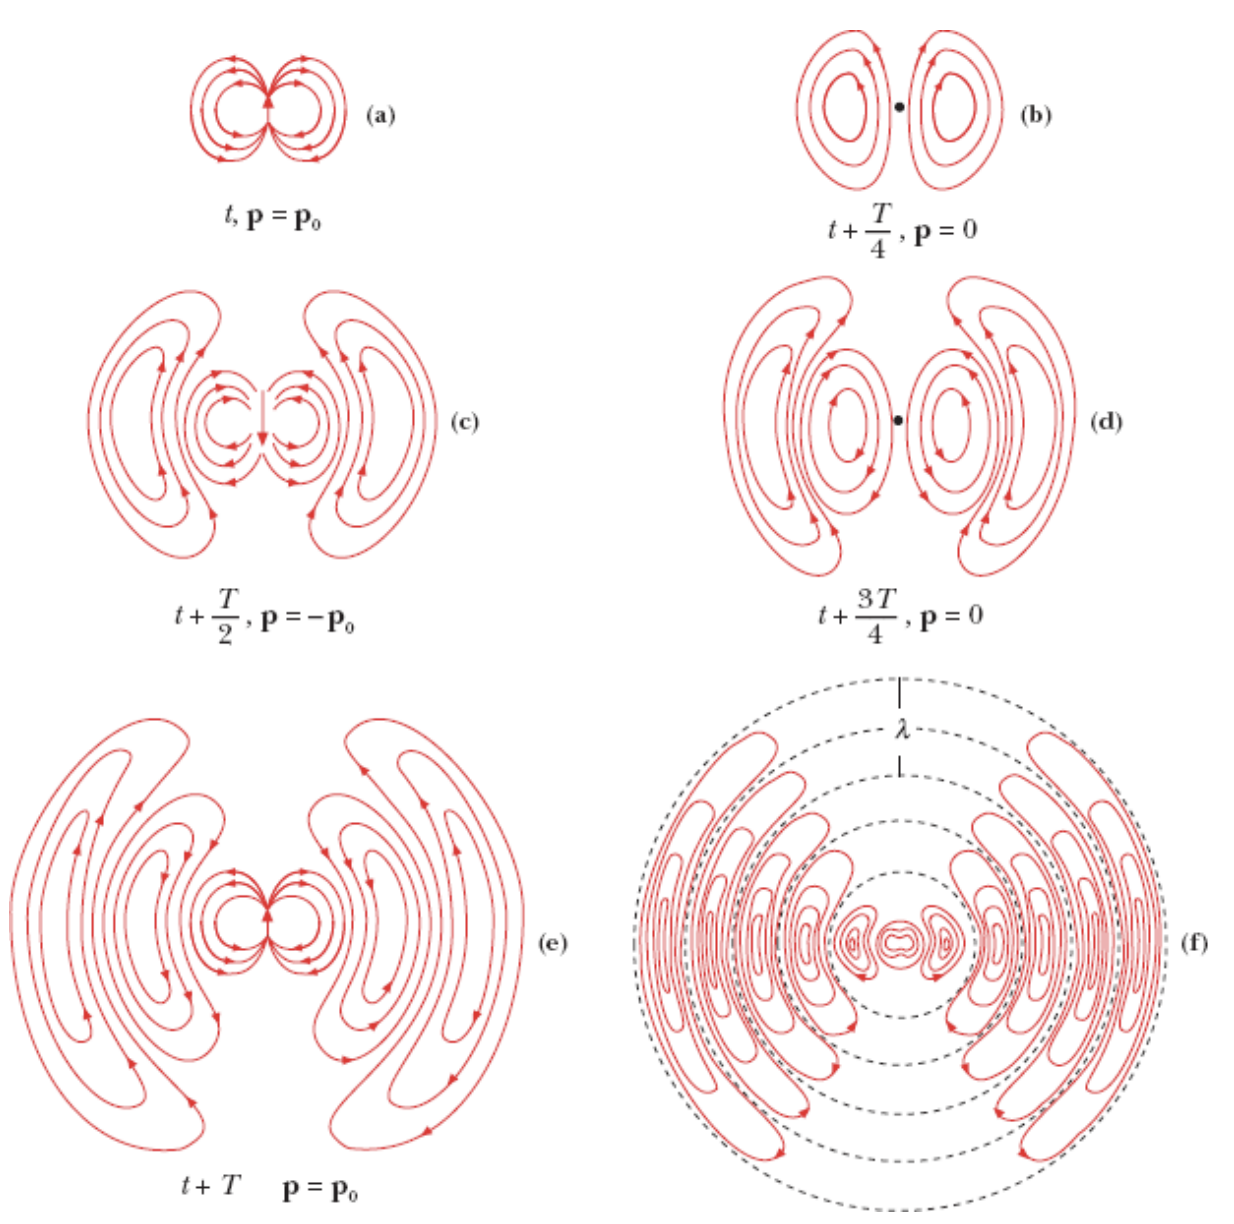
\includegraphics[width=0.65\linewidth]{figure/image69.png}
  \caption{Rappresentazione schematica della produzione e della propagazione delle linee di campo elettrico prodotte da un dipolo elettrico oscillante}
  \label{fig:etichetta}
\end{figure}

\newpage

\section{Termine di ordine successivo: dipolo magnetico e quadrupolo elettrico}

Come prima consideriamo una distribuzione di cariche e correnti monocromatica confinata in un volume piccolo ($d \ll \lambda$), ma ora includiamo il termine $n=1$ nello sviluppo \eqref{eq: sviluppo_multipoli_ritard}.
Il contributo di questo termine al potenziale vettore è 

\begin{equation}
    \mathbf{A}_1(\mathbf{r}) = \frac{\mu_0}{4 \pi} \frac{e^{ik}}{r} (-ikr) \int (\hat{r} \cdot \mathbf{r}')\mathbf{j}(\mathbf{r}') \ d^3 r'
\end{equation}

Includendo la dipendenza temporale e ricordando che $-ik = -i\omega/c = \partial_t/c$, si ha:

\begin{equation}
    \mathbf{A}_1(\mathbf{r}, t) = \frac{\mu_0}{4\pi c} \frac{\partial_t}{r} \int(\hat{r} \cdot \mathbf{r}') \mathbf{j} (\mathbf{r}', t_r) \ d^3 r'  
\end{equation}

\footnote{Attenzione, in questi appunti la notazione $t_r$, $[t']_{\text{rit}}$ hanno lo stesso significato, cioè indicano entrambe il tempo ritardato.} Per andare a semplificare l'integrale, scomponiamo l'integrando in parte simmetrica e antisimmetrica rispetto allo scambio $\hat{r} \leftrightarrow \mathbf{j}$:

\begin{align}
    (\hat{r} \cdot \mathbf{r'}) \mathbf{j} = \frac{1}{2}\left[(\hat{r} \cdot \mathbf{r'}) \mathbf{j} + (\hat{r} \cdot \mathbf{j}) \mathbf{r'}\right] + \frac{1}{2}\left[(\hat{r} \cdot \mathbf{r'}) \mathbf{j} - (\hat{r} \cdot \mathbf{j}) \mathbf{r'}\right]
\end{align}

Ricordando la \eqref{eq: integrale_momento_magnetico} il secondo termine si riscrive come

\begin{equation}
    \frac{1}{2}\left[(\hat{r} \cdot \mathbf{r'}) \mathbf{j} - (\hat{r} \cdot \mathbf{j}) \mathbf{r'}\right] = \frac{1}{2}(\mathbf{r'} \times \mathbf{j}) \times \hat{r}
\end{equation}

E quindi 

\begin{equation}
     (\hat{r} \cdot \mathbf{r'}) \mathbf{j} = \frac{1}{2}\left[(\hat{r} \cdot \mathbf{r'}) \mathbf{j} + (\hat{r} \cdot \mathbf{j}) \mathbf{r'}\right] + \frac{1}{2}(\mathbf{r'} \times \mathbf{j}) \times \hat{r}
\end{equation}

Questi due termini vanno analizzati separatamente, in quanto danno contributi fisicamente distinti.

\subsection{Dipolo magnetico oscillante}

Iniziamo con l'analizzare il secondo termine, e quindi consideriamo 

\begin{equation}
    \mathbf{A}_{M} = \frac{\mu_0}{4 \pi c} \frac{\partial_t}{r} \int \frac{1}{2} (\mathbf{r}' \times \mathbf{j}) \times \hat{r} \ d^3 r'
\end{equation}

Dalla definizione di momento magnetico data in magnetostatica \eqref{eq:momento_magnetico}, possiamo andare a definire il momento di dipolo magnetico generalizzato come:

\begin{tcolorbox}[colback=yellow!10!white, colframe=orange!70!black, boxrule=0.8pt]
\begin{equation}
    \mathbf{m}(t) = \frac{1}{2} \int \mathbf{r}' \times \mathbf{j}(\mathbf{r}', t) \, d^3r'
\end{equation}
\end{tcolorbox}

\newpage 

Pertanto il potenziale vettore riferito al secondo termine diventa 

\begin{tcolorbox}[colback=yellow!10!white, colframe=orange!70!black, boxrule=0.8pt]
\begin{equation}
    \mathbf{A}_{M} = \frac{\mu_0}{4 \pi c} \frac{\dot{\mathbf{m}}_r \times \hat{r}}{r}
\end{equation}
\end{tcolorbox}

dove $\mathbf{m}_r = \mathbf{m}(t - r/c)$ è il momento magnetico valutato al tempo ritardato. I campi di radiazione $(r \gg \lambda)$ risultano:

\begin{tcolorbox}[colback=yellow!10!white, colframe=orange!70!black, boxrule=0.8pt]
\begin{align}
    \mathbf{E}_{\text{rad}} &= \frac{\mu_0}{4\pi c} \frac{\ddot{\mathbf{m}}_r \times \hat{r}}{r} \label{eq: campo_elettrico_dip_magnetico}\\[6pt]
    \mathbf{B}_{\text{rad}} &= -\frac{\mu_0}{4\pi c^2} \frac{(\ddot{\mathbf{m}}_r \times \hat{r}) \label{eq: campo_magnetico_dip_magnetico} \times \hat{r}}{r}
\end{align}
\end{tcolorbox}

La struttura è formalmente identica a quella del dipolo elettrico \eqref{eq: E_rad_dipolo}--\eqref{eq: B_rad_dipolo}, con i ruoli di $\mathbf{E}$ e $\mathbf{B}$ scambiati e $\mathbf{p}$ sostituito da $\mathbf{m}/c$. 

\subsection{Quadrupolo elettrico oscillante}

Consideriamo ora il primo termine della decomposizione, la parte simmetrica:

\begin{equation}
    \mathbf{A}_{Q}(\mathbf{r}, t) = \frac{\mu_0}{4\pi c} \frac{\partial_t}{r} \int \frac{1}{2} \left[(\hat{r} \cdot \mathbf{r'}) \mathbf{j} + (\hat{r} \cdot \mathbf{j}) \mathbf{r'}\right] d^3r'
\end{equation}

Per valutare questo integrale utilizziamo l'equazione di continuità $\nabla \cdot \mathbf{j} = i\omega\rho$ e integriamo per parti. 
Si può dimostrare che:

\begin{equation}
    \int \frac{1}{2}\left[(\hat{r} \cdot \mathbf{r'}) \mathbf{j} + (\hat{r} \cdot \mathbf{j}) \mathbf{r'}\right] d^3r' = -\frac{i\omega}{2} \int \mathbf{r'}(\hat{r} \cdot \mathbf{r'}) \rho(\mathbf{r'}) \, d^3r' = -\frac{i\omega}{6} \, \dot{\mathbf{Q}}\hat{r}
\end{equation}

dove, ricordando la definizione \eqref{eq:tensore_quadrupolo}, abbiamo introdotto il \emph{tensore del momento di quadrupolo 
elettrico} a traccia nulla: \mkeyword{tensore del momento di 
quadrupolo elettrico}

\begin{tcolorbox}[colback=yellow!10!white, colframe=orange!70!black, 
boxrule=0.8pt]
\begin{equation}
    Q_{ij} (t) = \int \left(3r'_i r'_j - r'^2 \delta_{ij}\right) \rho(\mathbf{r'}, t) \, d^3r'
\end{equation}
\end{tcolorbox}

dove con $i$ e $j$ si va ad indicare due delle coordinate $x, y, z$ dell'elemento che si trova in $\mathbf{r}'$.\\

Il potenziale vettore del quadrupolo risulta quindi:

\begin{tcolorbox}[colback=yellow!10!white, colframe=orange!70!black, boxrule=0.8pt]
\begin{equation} \label{eq: potenziale_quadrupolo}
    \mathbf{A}_{Q}(\mathbf{r}, t) = \frac{\mu_0}{24\pi c} 
    \frac{\ddot{\mathbf{Q}}_r \cdot \hat{r}}{r}
\end{equation}
\end{tcolorbox}

dove $\mathbf{Q}_r$ indica il tensore valutato al tempo ritardato.

newpage

\section{Confronto tra dipolo elettrico e dipolo magnetico}

\'E istruttivo raccogliere i risultati ottenuti e confrontare la struttura dei campi dei due tipi di dipolo oscillante nella zona di radiazione:

\begin{center}
\renewcommand{\arraystretch}{2.4}
\begin{tabular}{lcc}
\hline
& \textbf{Dipolo elettrico} & \textbf{Dipolo magnetico} \\
\hline
$\mathbf{A}$ & 
$\dfrac{\mu_0}{4\pi}\dfrac{\dot{\mathbf{p}}_r}{r}$ & 
$\dfrac{\mu_0}{4\pi c}\dfrac{\dot{\mathbf{m}}_r \times \hat{r}}{r}$ 
\\[4pt]

$\mathbf{B}_\text{rad}$ & 
$\dfrac{\mu_0}{4\pi c}\dfrac{\ddot{\mathbf{p}}_r \times \hat{r}}{r}$ & 
$-\dfrac{\mu_0}{4\pi c^2}
\dfrac{(\ddot{\mathbf{m}}_r \times \hat{r}) \times \hat{r}}{r}$ \\[4pt]

$\mathbf{E}_\text{rad}$ & 
$\dfrac{\mu_0}{4\pi}
\dfrac{(\ddot{\mathbf{p}}_r \times \hat{r}) \times \hat{r}}{r}$ & 
$\dfrac{\mu_0}{4\pi c}\dfrac{\ddot{\mathbf{m}}_r \times \hat{r}}{r}$ \\
\hline
\end{tabular}
\end{center}

\vspace{0.5em}

La struttura è identica nei due casi, con i ruoli di $\mathbf{E}$ e $\mathbf{B}$ scambiati e $\mathbf{p}$ sostituito da $\mathbf{m}/c$, in accordo con la simmetria duale delle equazioni di Maxwell nel vuoto. 
Il fattore aggiuntivo $1/c$ nel dipolo magnetico implica che, a parità di ampiezza delle oscillazioni, la radiazione magnetica è soppressa rispetto a quella elettrica — il che spiega perché nelle sorgenti non relativistiche il dipolo elettrico domina sempre.\\

I potenziali ritardati costituiscono il punto di partenza per lo studio della radiazione elettromagnetica. 
Nel capitolo successivo vedremo come, a partire da questi risultati, sia possibile calcolare la potenza irradiata da ciascun multipolo e ricavare la formula di Larmor.

\chapter{Irraggiamento}

Quando le cariche \emph{accelerano}, i loro campi possono trasportare energia in modo \emph{irreversibile} all'infinito. Questo processo prende il nome di \emph{irraggiamento}. \footnote{In realtà è necessario fare una precisazione. Il termine più corretto da utilizzare sarebbe \emph{irraggiamento all'infinito}, in quanto, nel quotidiano, il termine irraggiamento viene usato (\emph{erroneamente}) riferendosi a una sorgente che emette energia sotto forma di onde elettromagnetiche, ma questa energia non viene necessariamente trasportata all'infinito. \\} \mkeyword{irraggiamento} \\

Più precisamente, diciamo che un sistema irradia quando il flusso del vettore di Poynting attraverso una superficie sferica di raggio $r$ rimane finito e non nullo nel limite $r \to \infty$:

\begin{equation}
    P_{\text{rad}} = \lim_{r \to \infty} \oint \mathbf{S} \cdot d \Sigma \ \mathbf{u}_n \neq 0
\end{equation}

Si nota allora che, dato che l'area è proporzionale a $r^2$, affinché ci sia irraggiamento è necessario che il vettore di Poynting non decada più velocemente di $1/r^2$. \\
Quindi per studiare l'irraggiamento è necessario considerare le parti di $\mathbf{E}$ e $\mathbf{B}$ che decadono come $1/r$ quando siamo in zona di radiazione ($d \ll \lambda \ll r$). \\

Adesso andremo ad analizzare l'irraggiamento di diversi tipi di sorgenti. 

\section{Irraggiamento di una carica puntiforme}

Supponiamo di considerare una carica puntiforme $q$ in moto con traiettoria $\mathbf{r}_q$ e velocità $\mathbf{v}(t) = \dot{\mathbf{r}}_q(t)$. Sappiamo che a questa sono associati i potenziali di Liènard-Wiechert \eqref{eq: potenziali_Liènard-Wiechert}. 
Grazie a questi è possibile ricavare il campo elettrico e il campo magnetico generati dalla carica, i quali risultano essere\footnote{Per vedere come si ricavano formalmente i campi guardare il capitolo 11 di \cite{IntroductiontoElectrodynamics}}:

\begin{tcolorbox}[colback=yellow!10!white, colframe=orange!70!black, boxrule=0.8pt]
\begin{align} 
    \mathbf{E}(\mathbf{r}, t) = \frac{q}{4 \pi \eps_0} \left[\frac{\mathcal{R}}{(\mathbf{\mathcal{R}} \cdot \mathbf{u})^3} \left[(c^2 (1 - \beta^2) \mathbf{u} + \mathbf{\mathcal{R}} \times (\mathbf{u} \times \mathbf{a}))\right] \right]_{\text{rit}} \label{eq: campo_elettrico_carica_moto}\\
    \mathbf{B}(\mathbf{r}, t) = \left[ \frac{1}{c} \hat{\mathcal{R}} \times \mathbf{E} \right]_{\text{rit}} \label{eq: campo_magnetico_carica_moto}
\end{align}
\end{tcolorbox}

\newpage

Dove abbiamo definito 

\begin{align*}
    \boldsymbol{\mathcal{R}} = \mathbf{r} - \mathbf{r}_q(t') \\
    \boldsymbol{\beta} = \frac{\mathbf{v}(t')}{c} \\
    \mathbf{u} = c \hat{\mathcal{R}} - \mathbf{v} = c (\hat{\mathcal{R}} - \mathbf{\beta})\\
    \mathbf{a} = \dot{\mathbf{v}}
\end{align*}

Allora il vettore di Poynting risulta essere 

\begin{equation} \label{eq: Poynting_irr}
    \mathbf{S} = \frac{1}{\mu_0} (\mathbf{E} \times \mathbf{B}) = \frac{1}{\mu_0 c} [\mathbf{E} \times (\hat{\mathbf{\mathcal{R}}} \times \mathbf{E})] = \frac{1}{\mu_0 c}[E^2 \hat{\mathbf{\mathcal{R}}} - (\hat{\mathbf{\mathcal{R}}} \cdot \mathbf{E})\mathbf{E}]
\end{equation}

Tuttavia non dobbiamo considerare tutti i termini del campo elettrico per trovare l'irraggiamento, una parte rappresenta l'energia di campo trasportata dalla particella durante il suo movimento. L'energia irradiata è quella che, di fatto, si \emph{stacca} dalla carica e si propaga all'infinito. \\

Per calcolare la potenza totale irradiata dalla particella al tempo $t_r$, consideriamo una sfera di raggio $\mathcal{R}$ centrata nella posizione della particella al tempo $t_r$. Dato che l'area della sfera è proporzionale a $\mathcal{R}^2$, tutti i termini in $\mathbf{S}$ che vanno come $1/\mathcal{R}^2$ daranno un contributo finito all'irraggiamento, tuttavia i termini come $1/\mathcal{R}^3$ o $1/\mathcal{R}^4$ daranno un contributo nullo per $\mathcal{R} \to \infty$.\\
Per questo \emph{nel campo elettrico solo il termine contenente l'accelerazione contribuisce alla radiazione}. 

\begin{equation}
    \mathbf{E}_{\text{rad}} = \frac{q}{4 \pi \eps_0} \frac{\mathcal{R}}{(\mathbf{{\mathcal{R}}} \cdot \mathbf{u})^3} [\mathbf{\mathcal{R}} \times (\mathbf{u} \times \mathbf{a})]
\end{equation}

Dato che $\mathbf{E}_\text{rad}$ è perpendicolare a $\hat{\mathbf{\mathcal{R}}}$, il secondo termine in \eqref{eq: Poynting_irr} scompare e quindi 

\begin{equation}
    \mathbf{S}_{\text{rad}} = \frac{1}{\mu_0 c} E_{\text{rad}}^2 \hat{\mathbf{\mathcal{R}}}
\end{equation}

Se la carica è istantaneamente a riposo, allora $\mathbf{u} = c \hat{\mathbf{\mathcal{R}}}$ e quindi

\begin{equation}
    \mathbf{E}_{\text{rad}} = \frac{q}{4 \pi \eps_0 c^2 \mathcal{R}} [\hat{\mathbf{\mathcal{R}}} \times (\hat{\mathbf{\mathcal{R}}} \times \mathbf{a})] = \frac{\mu_0 q}{4 \pi \mathcal{R}} [(\hat{\mathbf{\mathcal{R}}} \cdot \mathbf{a}) \hat{\mathbf{\mathcal{R}}} - \mathbf{a}]
\end{equation}

Sostituendo 

\begin{tcolorbox}[colback=yellow!10!white, colframe=orange!70!black, boxrule=0.8pt]
\begin{equation}
    \mathbf{S}_{\text{rad}} = \frac{1}{\mu_0 c} \left( \frac{\mu_0 q}{4 \pi \mathcal{R}} \right)^2 [a^2 - (\hat{\mathbf{\mathcal{R}}} \cdot \mathbf{a})^2] \hat{\mathbf{\mathcal{R}}} = \frac{\mu_0 q^2 a^2}{16 \pi^2 c} \left( \frac{\sin^2(\theta)}{\mathcal{R}^2} \right) \ \hat{\mathbf{\mathcal{R}}}
\end{equation}
\end{tcolorbox}

Allora la potenza totale irradiata è 

\begin{equation}
    P = \oint \mathbf{S}_{\text{rad}} \cdot d \Sigma \ \mathbf{u}_n = \frac{\mu_0 q^2 a^2}{16 \pi^2 c} \int \frac{\sin^2\theta}{\mathcal{R}^2} \mathcal{R}^2 \sin \theta \ d\theta \ d\phi
\end{equation}

La quale può essere scritta come 

\begin{tcolorbox}[colback=yellow!10!white, colframe=orange!70!black, boxrule=0.8pt]
\begin{equation} \label{eq: formula_Larmor}
    P = \frac{\mu_0 q^2 a^2}{6 \pi c}
\end{equation}\
\end{tcolorbox}

Questa è la \emph{formula di Larmor}: \mkeyword{formula di Larmor}qualsiasi carica accelerata irradia energia, con potenza proporzionale al quadrato dell'accelerazione. \\

La formula di Larmor ha implicazioni fisiche profonde: un elettrone classico in orbita attorno a un nucleo è continuamente accelerato centripetamente, quindi dovrebbe irraggiare energia e spiralare verso il nucleo in un tempo brevissimo. 
Questo è uno dei fallimenti fondamentali della fisica classica che ha portato allo sviluppo della meccanica quantistica.\\

Per ricavare questa relazione abbiamo supposto che la carica fosse istantaneamente ferma, tuttavia la \eqref{eq: formula_Larmor} continua a essere valida in buona approssimazione anche quando $v \ll c$. 

\subsection{Forza di reazione di radiazione}

\newpage

\section{Irraggiamento di un dipolo elettrico oscillante}

Consideriamo un dipolo elettrico oscillante. Dato che vogliamo calcolare l'irraggiamento del dipolo, ci interesseranno il campo elettrico e magnetico prodotti dal dipolo \emph{nella zona di radiazione}. 
Nel capitolo precedente abbiamo trovato che questi sono \eqref{eq: E_rad_dipolo} e \eqref{eq: B_rad_dipolo}. \\

Il vettore di Poynting è:

\begin{equation}
    \mathbf{S} = \frac{1}{\mu_0}(\mathbf{E}_{\text{rad}} \times \mathbf{B}_{\text{rad}})
\end{equation}

Per calcolarlo esplicitamente, notiamo che si ha $\mathbf{B}_{\text{rad}} = \frac{1}{c}\hat{r} \times \mathbf{E}_{\text{rad}}$, quindi:

\begin{equation}
    \mathbf{E}_{\text{rad}} \times \mathbf{B}_{\text{rad}} = \mathbf{E}_{\text{rad}} \times \left(\frac{1}{c}\hat{r} \times \mathbf{E}_{\text{rad}}\right) =\frac{1}{c}\left[E_{\text{rad}}^2 \hat{r} - (\mathbf{E}_{\text{rad}} \cdot \hat{r})\mathbf{E}_{\text{rad}}\right]
\end{equation}

Poiché nella zona di radiazione $\mathbf{E}_{\text{rad}} $ è ortogonale a $\hat{r}$ (il campo è trasversale), il secondo termine si annulla e si ottiene:

\begin{tcolorbox}[colback=yellow!10!white, colframe=orange!70!black,boxrule=0.8pt]
\begin{equation} \label{eq: Poynting_radiazione}
    \mathbf{S} = \frac{E_{\text{rad}}^2}{\mu_0 c} \hat{r} = \frac{\mu_0}{16\pi^2 c} \frac{|(\ddot{\mathbf{p}}_r \times \hat{r}) \times \hat{r}|^2}{r^2} \hat{r} = \frac{\mu_0}{16\pi^2 c}\frac{|\ddot{\mathbf{p}}_r |^2 \ \sin^2 \theta}{r^2} \hat{r}
\end{equation}
\end{tcolorbox}

Il vettore di Poynting è diretto radialmente verso l'esterno e decade come $r^{-2}$, garantendo la conservazione dell'energia: il flusso totale attraverso una sfera di raggio $r$ qualsiasi è indipendente da $r$.\\

L'intensità dell'onda, definita come la media sul periodo di $|\mathbf{S}|$, risulta essere 

\begin{tcolorbox}[colback=yellow!10!white, colframe=orange!70!black, boxrule=0.8pt]
\begin{equation}
    I(r,\theta) = \langle |\mathbf{S}| \rangle = \frac{\mu_0 \omega^4 p_0^2 }{32 \pi^2 c} \frac{\sin^2 \theta}{r^2} = \frac{I_0}{r^2} \sin^2 \theta
\end{equation}
\end{tcolorbox}

Dove abbiamo usato il fatto che $\langle \cos^2(\omega t) \rangle = 1/2$ e abbiamo definito 

\begin{tcolorbox}[colback=yellow!10!white, colframe=orange!70!black, boxrule=0.8pt]
\begin{equation}
    I_0 = \frac{\mu_0 p_0^2 \omega^4}{32 \pi^2 c}
\end{equation}
\end{tcolorbox}

Allora possiamo trovare la potenza totale irradiata integrando $I(r, \theta)$ sulla sfera di raggio $r$ (dove $r \to \infty$). 

\begin{equation}
    \langle P \rangle = \oint_{\Sigma} \langle \mathbf{S} \rangle \cdot d\Sigma \ \mathbf{u}_n = \frac{\mu_0 p_0^2 \omega^4}{32 \pi^2 c} \int_{0}^{2\pi} \int_{0}^{\pi} \frac{\sin^2 \theta}{r^2} r^2 \sin \theta \ d\theta \ d \phi = \frac{\mu_0 p_0^2 \omega^4}{12 \pi c}
\end{equation}

E quindi 

\begin{tcolorbox}[colback=yellow!10!white, colframe=orange!70!black, boxrule=0.8pt]
\begin{equation} \label{eq: potenza_dipolo_elettrico}
    \langle P \rangle = \frac{\mu_0 p_0^2 \omega^4}{12 \pi c} = \frac{8 \pi}{3} I_0
\end{equation}
\end{tcolorbox}

\subsection{Potenza irraggiata per unità di angolo solido}

A differenza di quanto abbiamo fatto sopra, adesso non andiamo a considerare tutta la superficie all'infinito, ma solo la parte di superficie $\Sigma$ che sottende un certo angolo solido $\Omega$. Allora si ha 

\begin{equation}
    \frac{d \langle P \rangle}{d \Omega} = \frac{d\langle P \rangle}{d\Sigma} \frac{d\Sigma}{d\Omega}
\end{equation}

Dato che $\Sigma = r^2 \ \Omega$ e $d\langle P \rangle/d\Sigma = I$, si ha

\begin{tcolorbox}[colback=yellow!10!white, colframe=orange!70!black, boxrule=0.8pt]
\begin{equation}
    \frac{d \langle P \rangle}{d \Omega} = I(r, \theta) \ r^2 = \frac{\mu_0 \omega^4 p_0^2}{32 \pi^2 c} \sin^2 \theta  = I_0 \sin^2 \theta
\end{equation}
\end{tcolorbox}

\subsection{Potenza istantanea}

Abbiamo trovato la potenza \emph{media} totale irradiata, tuttavia è possibile trovare anche la potenza \emph{istantanea} totale irradiata.

\begin{equation}
    P(t) = \oint_{\Sigma} \mathbf{S} \cdot d\Sigma \ \mathbf{u}_n = \frac{\mu_0 |\ddot{\mathbf{p}}_r|^2}{16 \pi^2 c} \int_0^{2\pi} \int_{0}^{\pi} \sin^3 \theta \ d\theta \ d\phi = \frac{\mu_0 |\ddot{\mathbf{p}}_r|^2}{6 \pi c} = \frac{\mu_0 p_0^2 \omega^4}{6 \pi c} \cos^2 (\omega t_r)
\end{equation}

Pertanto vale 

\begin{tcolorbox}[colback=yellow!10!white, colframe=orange!70!black, boxrule=0.8pt]
\begin{equation}
    P(t) = \frac{\mu_0 p_0^2 \omega^4}{6 \pi c} \cos^2 (\omega t_r)
\end{equation}
\end{tcolorbox}

Si nota, inoltre, che questo risultato è in perfetto accordo con quello trovato per la potenza media totale, in quanto $\langle \cos^2(\omega t_r)\rangle = 1/2$.

\section{Irraggiamento di un dipolo magnetico oscillante}

Consideriamo adesso un dipolo magnetico oscillante. Come fatto per il dipolo elettrico oscillante, anche in questo caso ci interessano il campo elettrico e magnetico prodotti dal dipolo \emph{nella zona di radiazione}, i quali abbiamo trovare essere \eqref{eq: campo_elettrico_dip_magnetico} e \eqref{eq: campo_magnetico_dip_magnetico}. \\
Seguendo i passaggi fatti prima si ha

\begin{equation}
    \mathbf{E}_{\text{rad}} \times \mathbf{B}_{\text{rad}} = \mathbf{E}_{\text{rad}} \times \left( \frac{1}{c} \hat{r} \times \mathbf{E}_{\text{rad}} \right) = \frac{1}{c} [E_{\text{rad}}^2 \hat{r} - (\mathbf{E}_{\text{rad}} \cdot \hat{r})\mathbf{E}_{\text{rad}}]
\end{equation}

Poiché $\mathbf{E}_{\text{rad}}$ è ortogonale a $\hat{r}$, il secondo termine si annulla e si ottiene:

\begin{tcolorbox}[colback=yellow!10!white, colframe=orange!70!black, boxrule=0.8pt]
\begin{equation}
    \mathbf{S} = \frac{E_{\text{rad}}^2}{\mu_0 c} \hat{r} = \frac{\mu_0}{16\pi^2 c^3} \frac{|\ddot{\mathbf{m}}_r \times \hat{r}|^2}{r^2} \hat{r} = \frac{\mu_0}{16\pi^2 c^3} \frac{|\ddot{\mathbf{m}}_r|^2 \sin^2\theta}{r^2} \hat{r}
\end{equation}
\end{tcolorbox}

\newpage

L'intensità media risulta:

\begin{tcolorbox}[colback=yellow!10!white, colframe=orange!70!black, boxrule=0.8pt]
\begin{equation}
    I(r, \theta) = \langle |\mathbf{S}| \rangle = \frac{\mu_0 \omega^4 m_0^2}{32\pi^2 c^3} \frac{\sin^2\theta}{r^2}
\end{equation}
\end{tcolorbox}

e la potenza totale media irradiata:

\begin{equation}
    \langle P \rangle = \frac{\mu_0 \omega^4 m_0^2}{32\pi^2 c^3} \int_0^{2\pi}\int_0^{\pi} \sin^3\theta \, d\theta \, d\phi = \frac{\mu_0 \omega^4 m_0^2}{12\pi c^3}
\end{equation}

E quindi

\begin{tcolorbox}[colback=yellow!10!white, colframe=orange!70!black, boxrule=0.8pt]
\begin{equation}\label{eq: potenza_dipolo_magnetico}
    \langle P \rangle = \frac{\mu_0 m_0^2 \omega^4}{12\pi c^3}
\end{equation}
\end{tcolorbox}

\subsection{Confronto tra irraggiamento del dipolo elettrico e del dipolo magnetico}

Si nota che la formula della potenzia media irraggiata dal dipolo magnetico è molto simile in forma a quella della potenzia media irraggiata dal dipolo elettrico (come ci si poteva aspettare), tuttavia esiste un'importante differenza tra le due: per configurazioni con dimensioni compatibili, la potenza elettrica irraggiata è enormemente maggiore. 
Confrontando le equazioni \eqref{eq: potenza_dipolo_magnetico} e \eqref{eq: potenza_dipolo_elettrico} 

\begin{equation}
    \frac{P_{\text{magnetico}}}{P_{\text{elettrico}}} = \left( \frac{m_0}{p_0 c} \right)^2
\end{equation}

Dove, ricordando che $m_0 = \pi b^2 I_0$ e $p_0 = q_0 d$ e ponendo $I = dq/dt$, cosa che implica $I_0 = q_0 \omega$, e considerando anche $d = \pi b$ (in modo da poter comparare le due grandezze), si ottiene

\begin{tcolorbox}[colback=yellow!10!white, colframe=orange!70!black, boxrule=0.8pt]
\begin{equation}
    \frac{P_{\text{magnetico}}}{P_{\text{elettrico}}} = \left( \frac{\omega b}{c} \right)^2
\end{equation}
\end{tcolorbox}

Ma il termine $c/\omega$ corrisponde alla lunghezza d'onda del dipolo (a meno di una costante) e dato che siamo in zona di radiazione, $b \ll c/\omega$, pertanto 

\begin{tcolorbox}[colback=yellow!10!white, colframe=orange!70!black, boxrule=0.8pt]
\begin{equation}
    P_{\text{magnetico}} \ll P_{\text{elettrico}} 
\end{equation}
\end{tcolorbox}

\section{Irraggiamento di una sorgente arbitraria}

\newpage 

\section{Irraggiamento atomico}

Oltre che dalle sorgenti "macroscopiche" e dalle sorgenti costituite da cariche libere accelerate, le onde elettromagnetiche hanno origine da fenomeni a livello atomico o nucleare.\\

Gli elettroni negli stati legati di singoli atomi liberi o di atomi aggregati in molecole possono essere eccitati, cioè ricevere un’energia $\Delta U$ pari al salto tra il livello energetico iniziale e quello finale: i meccanismi di eccitazione sono svariati, andando dagli urti dovuti al moto di agitazione termica agli urti con particelle cariche che attraversano il mezzo o con altri elettroni, come avviene in una scarica elettrica in un gas, e all’assorbimento di radiazione elettromagnetica.\\

Il modello atomico di Bohr è stato il primo che ha interpretato gli spettri di frequenze emessi dagli atomi e misurati sperimentalmente. In esso venne introdotta la struttura energetica discontinua caratterizzata da livelli discreti e ipotizzato l’assorbimento o l’emissione di radiazioni ogni qual volta un elettrone veniva eccitato o si diseccitava passando da un livello ad un altro. 

\begin{figure}[h]
  \centering
  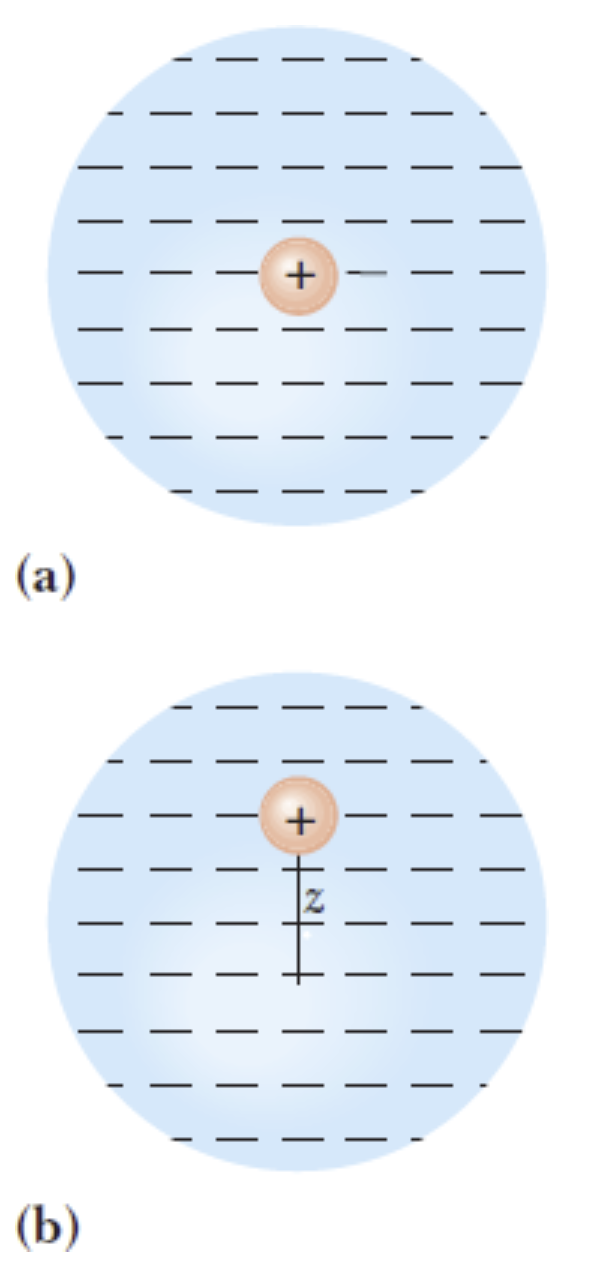
\includegraphics[width=0.25\linewidth]{figure/image70.png}
  \caption{Modello classico dell'atomo eccitato come oscillatore armonico}
  \label{fig:etichetta}
\end{figure}

Come sappiamo il modello di Bohr è stato poi superato da modelli quantistici più avanzati.\\

La \emph{luce visibile}, cui è sensibile la retina dell’occhio umano, è una particolare radiazione elettromagnetica emessa da atomi nel seguente campo di frequenze e di lunghezze d’onda (nel vuoto):

\begin{align}
    3.85 \cdot 10^{14} \leq \nu \leq 7.89 \cdot 10^{14} \ Hz\\
    2.42 \cdot 10^{15} \leq \omega \leq 4.96 \cdot 10^{15} \ \text{rad}/\text{s}\\
    0.78 \cdot 10^{-6} \geq \lambda \geq 0.38 \cdot 10^{-6} \ m
\end{align}

L’estremo superiore delle lunghezze d’onda, inferiore delle frequenze, corrisponde alla luce rossa, l’estremo inferiore delle lunghezze d’onda, superiore delle frequenze, alla luce violetta.\\

Malgrado l’impossibilità di fornire qui una spiegazione completa della radiazione di origine atomica, accenniamo lo stesso al modello classico dell’atomo come sorgente di radiazione affinché certi risultati siano utilizzabili per la comprensione almeno parziale di alcuni fenomeni.\\

Consideriamo il modello classico dell'atomo di idrogeno: un protone fermo circondato da una distribuzione sferica uniforme di carica negativa di raggio $R \sim 10^{-10}$ m. Il campo elettrico all'interno della sfera a distanza $z$ dal centro vale:

\begin{equation}
    E = \frac{\rho z}{3\varepsilon_0} = \frac{-e}{4\pi\varepsilon_0}\frac{z}{R^3} = \frac{ez}{4\pi\varepsilon_0 R^3}
\end{equation}

La forza di richiamo sull'elettrone è quindi armonica:

\begin{equation}
    F = -\frac{e^2}{4\pi\varepsilon_0 R^3}z = -Kz \quad \Rightarrow \quad \text{moto oscillatorio}
\end{equation}

con frequenza naturale:

\begin{equation}
    \omega_0 = \sqrt{\frac{K}{m_e}} = \sqrt{\frac{e^2}{4\pi\varepsilon_0 m_e R^3}} \approx 1.59 \times 10^{16}\text{ rad/s}
\end{equation}

che corrisponde a $\nu_0 \approx 2530$ THz, nel range dell'ultravioletto.\\

\subsection{Perdita di energia per irraggiamento}

La forza di reazione della radiazione su una carica oscillante vale:

\begin{equation}
    F_{\text{rad}} = \frac{\mu_0 q^2}{6\pi c} \dddot{z}
\end{equation}

Per oscillazioni quasi-monocromatiche $z \sim e^{-i\omega_0 t}$, si ha $\dddot{z} \approx -\omega_0^2\dot{z}$, quindi la forza di reazione è proporzionale alla velocità e si comporta come uno smorzamento viscoso:

\begin{equation}
    F_{\text{rad}} \approx -m_e\gamma_0\dot{z} \quad , \quad 
    \gamma_0 = \frac{\mu_0 q^2\omega_0^2}{6\pi m_e c} = 
    \frac{2r_e\omega_0^2}{3c}
\end{equation}

L'equazione del moto dell'elettrone diventa quella di un oscillatore armonico smorzato:

\begin{equation}
    \ddot{z} + \gamma_0\dot{z} + \omega_0^2 z = 0
\end{equation}

con soluzione:

\begin{equation}
    z(t) = z_0 e^{-\gamma_0 t/2}\cos(\omega' t) \quad , \quad \omega' = \sqrt{\omega_0^2 - \frac{\gamma_0^2}{4}} \approx \omega_0
\end{equation}

dove nell'ultima approssimazione abbiamo usato $\gamma_0 \ll \omega_0$, che si verifica essere $\gamma_0/\omega_0 \sim r_e/\lambda \sim 10^{-8}$.
Questa è l'\emph{approssimazione adiabatica}: il sistema perde energia molto lentamente rispetto al periodo di oscillazione. \mkeyword{approssimazione adiabatica}\\

L'energia meccanica del sistema decade quindi esponenzialmente:

\begin{tcolorbox}[colback=yellow!10!white, colframe=orange!70!black, boxrule=0.8pt]
\begin{equation}
    U(t) = \frac{1}{2}m_e\omega_0^2 z_0^2 e^{-\gamma_0 t} = U_0 e^{-t/\tau}
\end{equation}
\end{tcolorbox}

con tempo caratteristico di decadimento:

\begin{tcolorbox}[colback=yellow!10!white, colframe=orange!70!black, boxrule=0.8pt]
\begin{equation}
    \tau = \frac{1}{\gamma_0} = \frac{3c}{2r_e\omega_0^2} \approx 0.6 \text{ ns}
\end{equation}
\end{tcolorbox}

L'atomo emette quindi un pacchetto d'onda di durata $\sim\tau$, con larghezza spettrale associata:

\begin{equation}
    \Delta\nu = \frac{1}{2\pi\tau} \quad \Rightarrow \quad \frac{\Delta\nu}{\nu_0} = \frac{1}{2\pi\tau\nu_0} \approx 1.3\times10^{-7}
\end{equation}

Questo modello riproduce correttamente gli ordini di grandezza delle emissioni atomiche. La meccanica quantistica è necessaria per una descrizione precisa dei livelli energetici e delle frequenze di emissione, ma la fisica classica cattura bene la larghezza delle righe spettrali.

\subsection{Diffusione della luce}

Secondo il modello classico dell'atomo come oscillatore, quando un campo elettrico $\mathbf{E}$ variabile sinusoidalmente nel tempo, quale è quello associato a un'onda elettromagnetica armonica, agisce sull'atomo, l'equazione del moto diventa 

\begin{equation}
    m_e\ddot{z} + m_e\omega_0^2 z = eE_0 e^{-i\omega t}
\end{equation}

La soluzione \emph{stazionaria} è $z = z_0 e^{-i\omega t}$ con:

\begin{equation}
    z_0 = \frac{eE_0}{m_e(\omega_0^2 - \omega^2)}
\end{equation}

Il momento di dipolo indotto è $p_0 = ez_0 = \varepsilon_0\alpha_e E_0$, dove abbiamo definito la \emph{polarizzabilità elettronica} come: \mkeyword{polarizzabilità elettronica}

\begin{equation}
    \alpha_e = \frac{e^2}{\varepsilon_0 m_e(\omega_0^2 - \omega^2)}
\end{equation}

La potenza diffusa si ricava dalla \eqref{eq: potenza_dipolo_elettrico}:

\begin{equation}
    \langle P \rangle = \frac{\mu_0\omega^4}{12\pi c}p_0^2 = \frac{\mu_0\omega^4\varepsilon_0^2\alpha_e^2 E_0^2}{12\pi c}
\end{equation}

Per $\omega \ll \omega_0$ (luce visibile con $\omega_0$ nel range UV): $\alpha_e \approx e^2/(\varepsilon_0 m_e\omega_0^2)$ è costante e si ottiene la \emph{legge di Rayleigh}: \mkeyword{legge di Rayleigh}

\begin{tcolorbox}[colback=yellow!10!white, colframe=orange!70!black, boxrule=0.8pt]
\begin{equation}
    \langle P(\omega) \rangle \propto \omega^4 \propto \lambda^{-4}
\end{equation}
\end{tcolorbox}

Il rapporto tra la potenza diffusa dalla luce nel violetto ($\lambda \approx 380$ nm) e nel rosso ($\lambda \approx 780$ nm) vale:

\begin{equation}
    \frac{P_{\text{violetto}}}{P_{\text{rosso}}} = \left(\frac{\lambda_{\text{rosso}}}{\lambda_{\text{violetto}}}\right)^4 = \left(\frac{780}{380}\right)^4 \approx 18
\end{equation}

La luce viola e blu viene diffusa molto più efficacemente. Questo spiega due fenomeni familiari:

\begin{itemize}
    \item \textbf{Il cielo è azzurro}: la luce solare viene diffusa dall'atmosfera in tutte le direzioni e la componente blu/viola domina nell'irraggiamento diffuso.

    \item \textbf{Il tramonto è rosso}: la luce del sole al tramonto attraversa uno strato d'aria molto più spesso a causa dell'inclinazione; la componente blu viene quasi completamente diffusa via e rimane il rosso.
\end{itemize}

% \newpage

% .

% \newpage 



% In questo capitolo sfruttiamo i risultati ottenuti nel capitolo precedente
% per studiare il trasporto di energia da parte dei campi elettromagnetici
% generati da sorgenti oscillanti o in moto accelerato. Il punto di partenza
% sono i campi di radiazione ricavati per il dipolo elettrico oscillante
% \eqref{eq: E_rad_dipolo}--\eqref{eq: B_rad_dipolo}.

% \section{Potenza irradiata dal dipolo elettrico oscillante}

% \subsection{Vettore di Poynting nella zona di radiazione}

% Nella zona di radiazione ($r \gg \lambda$) i campi del dipolo elettrico
% oscillante sono:

% \begin{align}
%     \mathbf{E}_{\text{rad}} &= \frac{1}{4\pi\varepsilon_0 c^2}
%     \frac{(\ddot{\mathbf{p}}_r \times \hat{r}) \times \hat{r}}{r}
%     \label{eq: E_rad_cap} \\[6pt]
%     \mathbf{B}_{\text{rad}} &= \frac{\mu_0}{4\pi c}
%     \frac{\ddot{\mathbf{p}}_r \times \hat{r}}{r}
%     \label{eq: B_rad_cap}
% \end{align}

% Il vettore di Poynting è:

% \begin{equation}
%     \mathbf{S} = \frac{1}{\mu_0}(\mathbf{E}_{\text{rad}} \times
%     \mathbf{B}_{\text{rad}})
% \end{equation}

% Per calcolarlo esplicitamente, notiamo che dalla \eqref{eq: B_rad_cap}
% si ha $\mathbf{B}_{\text{rad}} = \frac{1}{c}\hat{r} \times
% \mathbf{E}_{\text{rad}}$, quindi:

% \begin{equation}
%     \mathbf{E}_{\text{rad}} \times \mathbf{B}_{\text{rad}} =
%     \mathbf{E}_{\text{rad}} \times \left(\frac{1}{c}\hat{r} \times
%     \mathbf{E}_{\text{rad}}\right) =
%     \frac{1}{c}\left[E_{\text{rad}}^2 \hat{r} -
%     (\mathbf{E}_{\text{rad}} \cdot \hat{r})\mathbf{E}_{\text{rad}}\right]
% \end{equation}

% Poiché nella zona di radiazione $\mathbf{E}_{\text{rad}} \perp \hat{r}$
% (il campo è trasversale), il secondo termine si annulla e si ottiene:

% \begin{tcolorbox}[colback=yellow!10!white, colframe=orange!70!black,
% boxrule=0.8pt]
% \begin{equation}\label{eq: Poynting_radiazione}
%     \mathbf{S} = \frac{E_{\text{rad}}^2}{\mu_0 c} \hat{r} =
%     \frac{\mu_0}{16\pi^2 c}
%     \frac{|(\ddot{\mathbf{p}}_r \times \hat{r}) \times \hat{r}|^2}
%     {r^2} \hat{r}
% \end{equation}
% \end{tcolorbox}

% Il vettore di Poynting è diretto radialmente verso l'esterno e decade
% come $r^{-2}$, garantendo la conservazione dell'energia: il flusso
% totale attraverso una sfera di raggio $r$ qualsiasi è indipendente
% da $r$.

% \subsection{Distribuzione angolare della potenza irradiata}

% La potenza irradiata per unità di angolo solido è:

% \begin{equation}
%     \frac{dP}{d\Omega} = |\mathbf{S}| r^2 =
%     \frac{\mu_0}{16\pi^2 c}
%     |(\ddot{\mathbf{p}}_r \times \hat{r}) \times \hat{r}|^2
% \end{equation}

% Supponiamo che il dipolo oscilli lungo $\hat{z}$, ovvero
% $\mathbf{p}(t) = p(t)\hat{z}$. Calcoliamo esplicitamente il doppio
% prodotto vettoriale. In coordinate sferiche con $\hat{z}$ come asse
% polare, il versore radiale è $\hat{r} = \sin\theta\cos\phi\,\hat{x}
% + \sin\theta\sin\phi\,\hat{y} + \cos\theta\,\hat{z}$, quindi:

% \begin{equation}
%     \ddot{\mathbf{p}}_r \times \hat{r} = \ddot{p}_r\hat{z} \times \hat{r}
%     = \ddot{p}_r(\hat{z} \times \hat{r})
% \end{equation}

% Per la geometria del problema $|\hat{z} \times \hat{r}| = \sin\theta$,
% e il doppio prodotto vettoriale dà la componente di $\ddot{\mathbf{p}}_r$
% trasversale a $\hat{r}$:

% \begin{equation}
%     |(\ddot{\mathbf{p}}_r \times \hat{r}) \times \hat{r}|^2 =
%     |\ddot{p}_r|^2 \sin^2\theta
% \end{equation}

% Pertanto:

% \begin{tcolorbox}[colback=yellow!10!white, colframe=orange!70!black,
% boxrule=0.8pt]
% \begin{equation}\label{eq: distribuzione_angolare}
%     \frac{dP}{d\Omega} = \frac{\mu_0}{16\pi^2 c}
%     |\ddot{p}_r|^2 \sin^2\theta
% \end{equation}
% \end{tcolorbox}

% Questo è il caratteristico \emph{pattern di irraggiamento del dipolo}:
% \mkeyword{pattern di irraggiamento} la radiazione è massima nel piano
% equatoriale ($\theta = \pi/2$, perpendicolare all'asse del dipolo) e
% si annulla lungo l'asse del dipolo ($\theta = 0, \pi$). Il pattern ha
% la forma di un toroide attorno all'asse $z$.

% \subsection{Potenza totale irradiata}

% Integriamo la distribuzione angolare \eqref{eq: distribuzione_angolare}
% su tutto l'angolo solido $d\Omega = \sin\theta\,d\theta\,d\phi$:

% \begin{equation}
%     P = \int \frac{dP}{d\Omega}\,d\Omega =
%     \frac{\mu_0}{16\pi^2 c} |\ddot{p}_r|^2
%     \int_0^{2\pi} d\phi \int_0^{\pi} \sin^3\theta\,d\theta
% \end{equation}

% L'integrale azimutale dà $2\pi$. Per quello polare, poniamo
% $u = \cos\theta$, $du = -\sin\theta\,d\theta$:

% \begin{equation}
%     \int_0^{\pi} \sin^3\theta\,d\theta =
%     \int_{-1}^{1} (1 - u^2)\,du =
%     \left[u - \frac{u^3}{3}\right]_{-1}^{1} =
%     \frac{2}{3} + \frac{2}{3} = \frac{4}{3}
% \end{equation}

% Quindi l'integrale totale vale $2\pi \cdot \frac{4}{3} = \frac{8\pi}{3}$,
% e la potenza istantanea irradiata è:

% \begin{tcolorbox}[colback=yellow!10!white, colframe=orange!70!black,
% boxrule=0.8pt]
% \begin{equation}\label{eq: potenza_istantanea_dipolo}
%     P_i(t) = \frac{\mu_0}{6\pi c} |\ddot{\mathbf{p}}_r|^2
% \end{equation}
% \end{tcolorbox}

% \subsection{Caso monocromatico e potenza media}

% Per oscillazioni monocromatiche $\mathbf{p}(t) = \mathbf{p}_0 e^{-i\omega t}$
% (con $\mathbf{p}_0$ reale), la derivata seconda al tempo ritardato è:

% \begin{equation}
%     \ddot{\mathbf{p}}_r = -\omega^2 \mathbf{p}_0 e^{-i\omega(t-r/c)}
%     \quad \Rightarrow \quad
%     |\ddot{\mathbf{p}}_r|^2 = \omega^4 p_0^2 \cos^2\omega(t - r/c)
% \end{equation}

% La media temporale su un periodo completo vale
% $\langle\cos^2\rangle = 1/2$, quindi:

% \begin{tcolorbox}[colback=yellow!10!white, colframe=orange!70!black,
% boxrule=0.8pt]
% \begin{align}
%     \left\langle\frac{dP}{d\Omega}\right\rangle &=
%     \frac{\mu_0 \omega^4 p_0^2}{32\pi^2 c} \sin^2\theta
%     \label{eq: dP_media} \\[8pt]
%     \langle P \rangle &= \frac{\mu_0 \omega^4 p_0^2}{12\pi c}
%     \label{eq: potenza_media_dipolo}
% \end{align}
% \end{tcolorbox}

% La dipendenza $\langle P \rangle \propto \omega^4$ è fondamentale:
% le sorgenti che oscillano a frequenza più alta irraggiano molto più
% efficacemente. Vedremo nella sezione sulla diffusione della luce che
% questa dipendenza è alla base del colore del cielo.

% \section{Formula di Larmor}

% \subsection{Derivazione}

% Consideriamo un sistema fisico elementare: una carica $q$ con
% accelerazione $\mathbf{a}(t)$, descritta nell'approssimazione di
% dipolo come $\ddot{\mathbf{p}} = q\mathbf{a}$. Sostituendo nella
% \eqref{eq: potenza_istantanea_dipolo}:

% \begin{tcolorbox}[colback=yellow!10!white, colframe=orange!70!black,
% boxrule=0.8pt]
% \begin{equation}\label{eq: Larmor}
%     P = \frac{\mu_0 q^2 a^2}{6\pi c} =
%     \frac{q^2 a^2}{6\pi\varepsilon_0 c^3}
% \end{equation}
% \end{tcolorbox}

% Questa è la \emph{formula di Larmor}: \mkeyword{formula di Larmor}
% qualsiasi carica accelerata irradia energia, con potenza proporzionale
% al quadrato dell'accelerazione. La formula di Larmor ha implicazioni
% fisiche profonde: un elettrone classico in orbita attorno a un nucleo
% è continuamente accelerato centripetamente, quindi dovrebbe irraggiare
% energia e spiralare verso il nucleo in un tempo brevissimo. Questo è
% uno dei fallimenti fondamentali della fisica classica che ha portato
% allo sviluppo della meccanica quantistica.

% \subsection{Generalizzazione relativistica}

% La formula di Larmor \eqref{eq: Larmor} vale nel limite non
% relativistico $v \ll c$. La sua generalizzazione relativistica,
% ricavabile dai potenziali di Liénard-Wiechert \eqref{potenziali
% ritardati}, è:

% \begin{tcolorbox}[colback=yellow!10!white, colframe=orange!70!black,
% boxrule=0.8pt]
% \begin{equation}\label{eq: Larmor_relativistica}
%     P = \frac{\mu_0 q^2 \gamma^6}{6\pi c}
%     \left(\dot{\beta}^2 -
%     |\boldsymbol{\beta} \times \dot{\boldsymbol{\beta}}|^2\right)
% \end{equation}
% \end{tcolorbox}

% che si riduce alla \eqref{eq: Larmor} per $\beta \to 0$
% ($\gamma \to 1$, $\dot{\boldsymbol{\beta}} \to \mathbf{a}/c$).
% Distinguiamo due casi fisicamente importanti.\\

% \textbf{Accelerazione parallela alla velocità}
% ($\boldsymbol{\beta} \parallel \dot{\boldsymbol{\beta}}$,
% acceleratore lineare): il termine $|\boldsymbol{\beta} \times
% \dot{\boldsymbol{\beta}}|^2 = 0$, quindi:

% \begin{equation}
%     P_{\parallel} = \frac{\mu_0 q^2 \gamma^6}{6\pi c} \dot{\beta}^2
% \end{equation}

% Il fattore $\gamma^6$ rende le perdite per irraggiamento enormi ad
% alte energie, rappresentando uno dei limiti fondamentali degli
% acceleratori lineari relativistici.\\

% \textbf{Accelerazione perpendicolare alla velocità}
% ($\boldsymbol{\beta} \perp \dot{\boldsymbol{\beta}}$, moto circolare):
% il termine $|\boldsymbol{\beta} \times \dot{\boldsymbol{\beta}}|^2 =
% \beta^2\dot{\beta}^2$, quindi:

% \begin{equation}
%     P_{\perp} = \frac{\mu_0 q^2 \gamma^6}{6\pi c}
%     (1 - \beta^2)\dot{\beta}^2 =
%     \frac{\mu_0 q^2 \gamma^4}{6\pi c} \dot{\beta}^2
% \end{equation}

% Questo fenomeno è detto \emph{radiazione di sincrotrone}.
% \mkeyword{radiazione di sincrotrone} Il fattore $\gamma^4$ implica
% perdite proibitive ad alte energie negli acceleratori circolari.\\

% Confrontando i due casi a parità di $\dot{\beta}$ e $\gamma$:

% \begin{equation}
%     \frac{P_{\parallel}}{P_{\perp}} = \gamma^2 \gg 1
% \end{equation}

% Quindi, ad alte energie, un acceleratore lineare perde per irraggiamento
% molto più di un acceleratore circolare, il che sembra controintuitivo
% ma è un fatto sperimentalmente ben verificato.

% \section{Dipolo di antenna}

% \subsection{Generalità}

% Un \emph{dipolo di antenna} \mkeyword{dipolo di antenna} è un filo
% conduttore di lunghezza $d$ con una distribuzione di corrente
% $I(z, t) = I_A(z)e^{-i\omega t}$. Nell'approssimazione $d \ll \lambda$
% il momento di dipolo si ricava dall'integrale:

% \begin{equation}
%     p_0 = \frac{i}{\omega}\int_{-d/2}^{d/2} I_A(z)\,dz
% \end{equation}

% che segue dalla definizione $\mathbf{p} = \int \rho\mathbf{r}\,d^3r$
% e dall'equazione di continuità $\partial_z I_A = i\omega\lambda_c$,
% dove $\lambda_c$ è la densità lineare di carica.\\

% La potenza totale irradiata si ricava dalla
% \eqref{eq: potenza_media_dipolo}:

% \begin{equation}
%     \langle P \rangle = \frac{\mu_0\omega^4}{12\pi c}|p_0|^2 =
%     \frac{Z_0\omega^4}{12\pi c^2}|p_0|^2
% \end{equation}

% Si definisce la \emph{resistenza di antenna} \mkeyword{resistenza di
% antenna} come la resistenza equivalente che dissiperebbe la stessa
% potenza per effetto Joule:

% \begin{equation}
%     \langle P \rangle = \frac{1}{2}R_{\text{ant}}I_{A0}^2
%     \quad \Rightarrow \quad
%     R_{\text{ant}} = \frac{2\langle P \rangle}{I_{A0}^2}
% \end{equation}

% \subsection{Caso a: carica solo alle estremità}

% La corrente è costante lungo il filo: $I_A(z) = I_{A0}$. L'integrale
% del momento di dipolo dà:

% \begin{equation}
%     p_0 = \frac{i}{\omega}\int_{-d/2}^{d/2} I_{A0}\,dz =
%     \frac{iI_{A0}d}{\omega}
% \end{equation}

% quindi $|p_0|^2 = I_{A0}^2 d^2/\omega^2$ e la potenza vale:

% \begin{equation}
%     \langle P \rangle = \frac{Z_0\omega^4}{12\pi c^2}
%     \frac{I_{A0}^2 d^2}{\omega^2} =
%     \frac{Z_0\omega^2 d^2}{12\pi c^2} I_{A0}^2
% \end{equation}

% La resistenza di antenna risulta:

% \begin{tcolorbox}[colback=yellow!10!white, colframe=orange!70!black,
% boxrule=0.8pt]
% \begin{equation}
%     R_{\text{ant}} = \frac{Z_0\omega^2 d^2}{6\pi c^2} =
%     \frac{2\pi Z_0}{3}\left(\frac{d}{\lambda}\right)^2
% \end{equation}
% \end{tcolorbox}

% \subsection{Caso b: corrente triangolare}

% La distribuzione di corrente si annulla alle estremità linearmente:
% $I_A(z) = I_{A0}(1 - 2|z|/d)$. L'integrale vale:

% \begin{equation}
%     \int_{-d/2}^{d/2} I_{A0}\left(1 - \frac{2|z|}{d}\right)dz =
%     2I_{A0}\int_0^{d/2}\left(1 - \frac{2z}{d}\right)dz =
%     2I_{A0}\left[\frac{d}{2} - \frac{d}{4}\right] =
%     \frac{I_{A0}d}{2}
% \end{equation}

% quindi $p_0 = iI_{A0}d/(2\omega)$, cioè la metà del caso precedente.
% Poiché la potenza scala con $|p_0|^2$, risulta un quarto:

% \begin{tcolorbox}[colback=yellow!10!white, colframe=orange!70!black,
% boxrule=0.8pt]
% \begin{equation}
%     R_{\text{ant}} = \frac{\pi Z_0}{6}\left(\frac{d}{\lambda}\right)^2
%     \approx 197\,\Omega\left(\frac{d}{\lambda}\right)^2
% \end{equation}
% \end{tcolorbox}

% \subsection{Caso c: onda stazionaria con nodi alle estremità ($d = \lambda/2$)}

% La distribuzione di corrente è sinusoidale con nodi alle estremità:
% $I_A(z) = I_{A0}\sin(k(d/2 - |z|))$. Questo è il caso dell'antenna
% a mezza lunghezza d'onda, la geometria più comune nelle applicazioni
% pratiche.\\

% Calcoliamo l'integrale del momento di dipolo con $k = \omega/c$:

% \begin{equation}
%     \int_{-d/2}^{d/2} I_{A0}\sin\left(k\left(\frac{d}{2} -
%     |z|\right)\right)dz =
%     2I_{A0}\int_0^{d/2}\sin\left(k\left(\frac{d}{2} - z\right)\right)dz
% \end{equation}

% Con la sostituzione $u = k(d/2 - z)$, $du = -k\,dz$:

% \begin{equation}
%     = \frac{2I_{A0}}{k}\int_0^{kd/2}\sin(u)\,du =
%     \frac{2I_{A0}}{k}[-\cos u]_0^{kd/2} =
%     \frac{2I_{A0}}{k}(1 - \cos(kd/2))
% \end{equation}

% Per $d = \lambda/2$, si ha $kd/2 = \pi/2$, quindi $\cos(kd/2) = 0$ e:

% \begin{equation}
%     \int_{-d/2}^{d/2} I_A(z)\,dz = \frac{2I_{A0}}{k} =
%     \frac{2I_{A0}c}{\omega}
% \end{equation}

% Il momento di dipolo è $p_0 = \frac{i}{\omega} \cdot
% \frac{2I_{A0}c}{\omega} = \frac{2iI_{A0}c}{\omega^2}$, e la potenza vale:

% \begin{equation}
%     \langle P \rangle = \frac{Z_0\omega^4}{12\pi c^2} \cdot
%     \frac{4I_{A0}^2 c^2}{\omega^4} = \frac{Z_0}{3\pi}I_{A0}^2
% \end{equation}

% La resistenza di antenna per l'antenna a $\lambda/2$ è:

% \begin{tcolorbox}[colback=yellow!10!white, colframe=orange!70!black,
% boxrule=0.8pt]
% \begin{equation}
%     R_{\text{ant}} = \frac{2Z_0}{3\pi} \approx 80\,\Omega
% \end{equation}
% \end{tcolorbox}

% Il valore $R \approx 80\,\Omega$ è un risultato fondamentale
% dell'ingegneria delle antenne: un'antenna a dipolo di mezza lunghezza
% d'onda ha una resistenza di antenna di circa $80\,\Omega$,
% indipendentemente dalla frequenza di operazione.

% \section{Modello classico dell'atomo e irraggiamento atomico}

% \subsection{Modello dell'atomo di idrogeno}

% Consideriamo il modello classico dell'atomo di idrogeno: un protone
% fermo circondato da una distribuzione sferica uniforme di carica
% negativa di raggio $R \sim 10^{-10}$ m. Il campo elettrico all'interno
% della sfera a distanza $z$ dal centro vale:

% \begin{equation}
%     E = \frac{\rho z}{3\varepsilon_0} =
%     \frac{-e}{4\pi\varepsilon_0}\frac{z}{R^3} =
%     \frac{ez}{4\pi\varepsilon_0 R^3}
% \end{equation}

% La forza di richiamo sull'elettrone è quindi armonica:

% \begin{equation}
%     F = -\frac{e^2}{4\pi\varepsilon_0 R^3}z = -Kz
%     \quad \Rightarrow \quad \text{moto oscillatorio}
% \end{equation}

% con frequenza naturale:

% \begin{equation}
%     \omega_0 = \sqrt{\frac{K}{m_e}} =
%     \sqrt{\frac{e^2}{4\pi\varepsilon_0 m_e R^3}}
%     \approx 1.59 \times 10^{16}\text{ rad/s}
% \end{equation}

% che corrisponde a $\nu_0 \approx 2530$ THz, nel range dell'ultravioletto.\\

% \subsection{Perdita di energia per irraggiamento}

% Se $z_0$ è l'ampiezza di oscillazione, il momento di dipolo vale
% $p_0 = ez_0$ e l'energia meccanica del sistema è:

% \begin{equation}
%     U = \frac{1}{2}m_e\omega_0^2 z_0^2
% \end{equation}

% La potenza media irradiata per la formula di Larmor
% \eqref{eq: Larmor} con $\langle a^2 \rangle = \omega_0^4 z_0^2/2$:

% \begin{equation}
%     \langle P \rangle = \frac{\mu_0 q^2}{6\pi c}
%     \frac{\omega_0^4 z_0^2}{2} =
%     \frac{e^2\omega_0^4 z_0^2}{12\pi\varepsilon_0 c^3}
% \end{equation}

% Introduciamo il \emph{raggio classico dell'elettrone}:
% \mkeyword{raggio classico dell'elettrone}

% \begin{tcolorbox}[colback=yellow!10!white, colframe=orange!70!black,
% boxrule=0.8pt]
% \begin{equation}
%     r_e = \frac{e^2}{4\pi\varepsilon_0 m_e c^2} \approx 2.8\text{ fm}
% \end{equation}
% \end{tcolorbox}

% In termini di $r_e$ la potenza si riscrive come:

% \begin{equation}
%     \langle P \rangle =
%     \frac{2r_e\omega_0^2}{3c} \cdot
%     \frac{1}{2}m_e\omega_0^2 z_0^2 =
%     \frac{2r_e\omega_0^2}{3c} U
% \end{equation}

% La perdita di energia per irraggiamento soddisfa l'equazione
% differenziale:

% \begin{equation}
%     \frac{dU}{dt} = -\langle P \rangle = -\frac{2r_e\omega_0^2}{3c} U
% \end{equation}

% con soluzione $U(t) = U_0 e^{-t/\tau}$ e tempo caratteristico:

% \begin{tcolorbox}[colback=yellow!10!white, colframe=orange!70!black,
% boxrule=0.8pt]
% \begin{equation}
%     \tau = \frac{3c}{2r_e\omega_0^2} \approx 0.6\text{ ns}
% \end{equation}
% \end{tcolorbox}

% L'atomo emette quindi un pacchetto d'onda di durata $\sim\tau$. La
% larghezza spettrale associata è:

% \begin{equation}
%     \Delta\nu = \frac{1}{2\pi\tau}
%     \quad \Rightarrow \quad
%     \frac{\Delta\nu}{\nu_0} = \frac{1}{2\pi\tau\nu_0} \approx
%     1.3 \times 10^{-7}
% \end{equation}

% Questo modello riproduce correttamente gli ordini di grandezza delle
% emissioni atomiche. La meccanica quantistica è necessaria per una
% descrizione precisa dei livelli energetici e delle frequenze di
% emissione, ma la fisica classica cattura bene la larghezza delle righe
% spettrali.

% \section{Diffusione della luce}

% \subsection{Scattering di Thomson}

% Consideriamo un elettrone \emph{libero} investito da un'onda
% elettromagnetica piana monocromatica con campo elettrico
% $\mathbf{E} = \mathbf{E}_0 e^{-i\omega t}$ (trascuriamo la forza
% magnetica di Lorentz in quanto di ordine $v/c$ rispetto a quella
% elettrica). L'equazione del moto dell'elettrone è:

% \begin{equation}
%     m_e\ddot{\mathbf{r}} = e\mathbf{E}_0 e^{-i\omega t}
%     \quad \Rightarrow \quad
%     \mathbf{a} = \frac{e\mathbf{E}_0}{m_e}e^{-i\omega t}
% \end{equation}

% con $\langle a^2\rangle = e^2 E_0^2/(2m_e^2)$. Per la formula di
% Larmor la potenza diffusa è:

% \begin{equation}
%     P_{\text{diff}} = \frac{\mu_0 e^2}{6\pi c}\langle a^2\rangle =
%     \frac{\mu_0 e^2}{6\pi c} \cdot \frac{e^2 E_0^2}{2m_e^2} =
%     \frac{\mu_0 e^4 E_0^2}{12\pi m_e^2 c}
% \end{equation}

% L'intensità dell'onda incidente è:

% \begin{equation}
%     I_0 = \langle|\mathbf{S}|\rangle =
%     \frac{1}{2}\varepsilon_0 c E_0^2 =
%     \frac{E_0^2}{2\mu_0 c}
% \end{equation}

% La \emph{sezione d'urto di diffusione} \mkeyword{sezione d'urto di
% diffusione} è definita come il rapporto tra potenza diffusa e
% intensità incidente, e ha le dimensioni di un'area:

% \begin{equation}
%     \sigma_T = \frac{P_{\text{diff}}}{I_0} =
%     \frac{\mu_0 e^4 E_0^2}{12\pi m_e^2 c} \cdot
%     \frac{2\mu_0 c}{E_0^2} =
%     \frac{\mu_0^2 e^4}{6\pi m_e^2}
% \end{equation}

% Riscrivendo in termini del raggio classico dell'elettrone
% $r_e = \mu_0 e^2/(4\pi m_e)$:

% \begin{tcolorbox}[colback=yellow!10!white, colframe=orange!70!black,
% boxrule=0.8pt]
% \begin{equation}\label{eq: sezione_urto_Thomson}
%     \sigma_T = \frac{8\pi}{3}r_e^2 \approx 0.66\times10^{-28}\text{ m}^2
% \end{equation}
% \end{tcolorbox}

% Questa è la \emph{sezione d'urto di Thomson}. \mkeyword{sezione d'urto
% di Thomson} Notare che $\sigma_T$ non dipende da $\omega$: un elettrone
% libero diffonde tutte le frequenze con la stessa efficienza. L'unità
% $10^{-28}$ m$^2 = 10^{-24}$ cm$^2$ prende il nome di \emph{barn}
% \mkeyword{barn} ed è l'unità standard in fisica nucleare e delle
% particelle. Questo risultato descrive correttamente la diffusione per
% $h\nu \ll m_e c^2$ (cioè $\nu \lesssim 10^{20}$ Hz); a energie più
% alte entrano in gioco effetti quantistici descritti dalla sezione
% d'urto di Klein-Nishina.

% \subsection{Diffusione di Rayleigh}

% Per la diffusione da atomi, l'elettrone non è libero ma legato con
% frequenza di risonanza $\omega_0$. L'equazione del moto diventa:

% \begin{equation}
%     m_e\ddot{z} + m_e\omega_0^2 z = eE_0 e^{-i\omega t}
% \end{equation}

% La soluzione stazionaria è $z = z_0 e^{-i\omega t}$ con:

% \begin{equation}
%     z_0 = \frac{eE_0/m_e}{\omega_0^2 - \omega^2}
% \end{equation}

% Il momento di dipolo indotto è $p_0 = ez_0 = \varepsilon_0\alpha_e E_0$,
% dove la \emph{polarizzabilità elettronica} vale:
% \mkeyword{polarizzabilità elettronica}

% \begin{equation}
%     \alpha_e = \frac{e^2}{\varepsilon_0 m_e(\omega_0^2 - \omega^2)}
% \end{equation}

% La potenza diffusa si ricava dalla \eqref{eq: potenza_media_dipolo}:

% \begin{equation}
%     \langle P \rangle = \frac{\mu_0\omega^4}{12\pi c}p_0^2 =
%     \frac{\mu_0\omega^4\varepsilon_0^2\alpha_e^2 E_0^2}{12\pi c}
% \end{equation}

% La sezione d'urto di Rayleigh è quindi:

% \begin{equation}
%     \sigma_R = \frac{\langle P\rangle}{I_0} =
%     \frac{\mu_0\omega^4\varepsilon_0^2\alpha_e^2 E_0^2}{12\pi c} \cdot
%     \frac{2}{  \varepsilon_0 c E_0^2} \propto \omega^4\alpha_e^2
% \end{equation}

% Per $\omega \ll \omega_0$ (luce visibile con $\omega_0$ nel range UV):
% $\alpha_e \approx e^2/(\varepsilon_0 m_e\omega_0^2)$ è costante e si
% ottiene la \emph{legge di Rayleigh}: \mkeyword{legge di Rayleigh}

% \begin{tcolorbox}[colback=yellow!10!white, colframe=orange!70!black,
% boxrule=0.8pt]
% \begin{equation}
%     \sigma_R \propto \omega^4 \propto \lambda^{-4}
% \end{equation}
% \end{tcolorbox}

% Il rapporto tra luce diffusa nel violetto ($\lambda \approx 380$ nm)
% e nel rosso ($\lambda \approx 780$ nm) vale:

% \begin{equation}
%     \frac{\sigma_{\text{violetto}}}{\sigma_{\text{rosso}}} =
%     \left(\frac{\lambda_{\text{rosso}}}{\lambda_{\text{violetto}}}
%     \right)^4 = \left(\frac{780}{380}\right)^4 \approx 7\div 10
% \end{equation}

% La luce viola e blu viene diffusa molto più efficacemente. Questo
% spiega due fenomeni familiari:

% \begin{itemize}
%     \item \textbf{Il cielo è azzurro}: la luce solare viene diffusa
%     dall'atmosfera in tutte le direzioni e la componente blu/viola
%     domina nell'irraggiamento diffuso.

%     \item \textbf{Il tramonto è rosso}: la luce del sole attraversa
%     uno strato d'aria molto più spesso; la componente blu viene
%     quasi completamente diffusa via e rimane il rosso.
% \end{itemize}

% \subsection{Polarizzazione della luce diffusa}

% Nella zona di radiazione il campo $\mathbf{E}_{\text{rad}}$ è
% proporzionale alla componente di $\ddot{\mathbf{p}}_r$ trasversale
% a $\hat{r}$, ovvero $\mathbf{E}_{\text{rad}} \propto
% (\ddot{\mathbf{p}}_r \times \hat{r}) \times \hat{r} =
% \ddot{\mathbf{p}}_{r,\perp}$.\\

% Consideriamo un'onda incidente lungo $\hat{z}$ con polarizzazione
% lungo $\hat{x}$: il dipolo indotto oscilla lungo $\hat{x}$. La luce
% diffusa nella direzione $\hat{y}$ (perpendicolare a $\hat{z}$ e
% $\hat{x}$) ha la componente di $\ddot{\mathbf{p}}$ trasversale a
% $\hat{y}$ che è tutta lungo $\hat{x}$: la luce è
% \emph{completamente polarizzata linearmente} lungo $\hat{x}$.\\

% Per luce incidente non polarizzata, la media sulle polarizzazioni dà luce diffusa a $90°$ \emph{parzialmente polarizzata}. 
% Questo effetto è osservabile guardando il cielo con un filtro polarizzatore: in direzione perpendicolare al sole, la luce è parzialmente polarizzata.

\printbibliography

\end{document}
